\chapter{Trigger efficiency measurement} \label{appendix:triggerefficiency}
In this appendix is presented more information, omitted in section~\ref{sec:trigger}, regarding the measurement of the trigger efficiency in data and simulation. 

An event selection to get an enriched sample of $\ttbar$ events with a dileptonic final state ($\mathrm{\ttbar \rightarrow W^{+}b W^{-}b \rightarrow e^{\pm} {\nu}_{e} \mu^{\mp}{\nu}_{\mu}}$) is applied for the measurement. First, events pass the HLT\_IsoMu24 trigger path. They must contain exactly muon with $\pt > 30$ GeV satisfying the medium identification working point and a PF relative isolation $< 0.1$. Events are vetoed if they contain additional muons of relative isolation $< 0.3$ with the same $\pt$ and identification criteria. Events are also required to contain an electron with $\pt > 10$ GeV, relative isolation $< 0.1$. The electron and muon are required to have opposite electric charge.  Events are also required to have at least 4 jets with $\pt > 25$ GeV, $|\eta|<$ 2.4, the tight working point of the jet ID algorithm, deepJet score $>0$. Selected jets with $\pt< 50$ GeV are requested to pass the medium working point of the PU ID algorithm. The four jets with the highest deepJet score are selected. The trigger objects passing the required filters are counted only if they are matched within $\Delta R$ = 0.5 with the four jets. This last requirement is not applied to filters applied on the HT since it is a property of the event and not of the single jets.

The filters associated to the HLT trigger paths used in three years are shown in tables \ref{trigger:tab:filters2016Double}, \ref{trigger:tab:filters2016Quad}, \ref{trigger:tab:filters2017} and \ref{trigger:tab:filters2018}. The efficiency for each filter as measured in data and in simulation is shown in Figures~\ref{trigger:fig:filterEfficiency2016DoubleOverlap}, \ref{trigger:fig:filterEfficiency2016QuadOverlap}, and~\ref{trigger:fig:filterEfficiency2016AndOverlap} for 2016, in Figures~\ref{trigger:fig:filterEfficiency2017} for 2017, and in Figures~\ref{trigger:fig:filterEfficiency2018} for 2018. The efficiency measurement has the important subtleties to mention: 
\begin{itemize}
    \item The nominal procedure cannot be applied directly to filters with b-tagging requirements because there are only two jets which are real b-jets in $\ttbar$ events. Consequently, the efficiency of an online b-tag is evaluated by selecting the highest b-tagged jet (the most probable one to be a real b-jet) of the event and checking that it matches a trigger object passing the online b-tag. Then the triple b-tagging filter efficiency is evaluated as the probability that three out of the four selected jets pass online b-tag.
    \item  The 2016 trigger requirements are the logical `OR' of two paths. Hence, the efficiency of the OR is evaluated using equation~\ref{eq:triggeror}, where $\mathrm{\epsilon(Double90Quad30~\&~Quad45) = \epsilon(Double90Quad30)~x~\epsilon'(Quad45)}$, with $\mathrm{\epsilon'(Quad45)}$ defined as the efficiency of the `Quad45' trigger over a sample of events passing the `Double90Quad30' trigger.
\end{itemize}
\begin{equation} 
\mathrm{\epsilon (OR) = \epsilon(Double90Quad30) + \epsilon(Quad45) - \epsilon(Double90Quad30 \& Quad45)}
\label{eq:triggeror}
\end{equation}

\begin{table}[ht!]
\caption[Filters of the HLT\_DoubleJet90\_Double30\_TripleBTagCSV trigger path in the 2016 dataset]{\label{trigger:tab:filters2016Double}Filters associated to the HLT\_DoubleJet90\_Double30\_TripleBTagCSV trigger path in the 2016 dataset. The filters are sorted in the order of their application. The number of objects required and the variable as a function of which the efficiency is measured are shown.}
\centering
\begin{tabularx}{\textwidth}{lXX}
    \hline
    \small Filter name &\small \# of required objects    &\small Variable  \\
    \hline
    \small hltL1sTripleJetVBFIorHTTIorDoubleJetCIorSingleJet &\small 1 &\small $\sum_{jet} p_T$ \\
    \small hltQuadCentralJet30 &\small 4 &\small $p_T^4$ \\ 
    \small hltDoubleCentralJet90 &\small 2 &\small $p_T^2$ \\ 
    \small hltBTagCaloCSVp087Triple &\small 3 &\small see text \\ 
    \small hltQuadPFCentralJetLooseID30 &\small 4 &\small $p_T^4$ \\
    \small hltDoublePFCentralJetLooseID90 &\small 2 &\small $p_T^2$ \\
    \hline
\end{tabularx}
\end{table}

\begin{table}[ht!]
\caption[Filters of the HLT\_QuadJet45\_TripleBTagCSV trigger path in the 2016 dataset]{\label{trigger:tab:filters2016Quad}Filters of the HLT\_QuadJet45\_TripleBTagCSV trigger path in the 2016 dataset. The filters are sorted following the order of their application. The number of objects required and the variable as a function of which the efficiency is measured are shown.}
\centering
\begin{tabularx}{\textwidth}{lXX}
    \hline
    \small Filter name &\small \# of objects    &\small Variable  \\
    \hline
    \small hltL1sQuadJetCIorTripleJetVBFIorHTT &\small 1 &\small $\sum_{jet} p_T$ \\
    \small hltQuadCentralJet45 &\small 4 &\small $p_T^4$ \\ 
    \small hltBTagCaloCSVp087Triple &\small 3 &\small see text \\ 
    \small hltQuadPFCentralJetLooseID45 &\small 4 &\small $p_T^4$ \\
    \hline
\end{tabularx}
\end{table}

\begin{table}[ht!]
\caption[Filters of the HLT\_PFHT300PT30\_QuadPFJet\_75\_60\_45\_40\_TriplePFBTagCSV trigger path in 2017 dataset]{\label{trigger:tab:filters2017}Filters of the HLT\_PFHT300PT30\_QuadPFJet\_75\_60\_45\_40\_TriplePFBTagCSV trigger path in 2017 dataset. The filters are sorted following the order of their application. For every filter, the number of objects required and the variable as a function of which the efficiency is measures is reported.}
\centering
\begin{tabularx}{\textwidth}{lXX}
    \hline
    \small Filter name &\small \# of objects    &\small Variable  \\
    \hline    
    \small hltL1sQuadJetC60IorHTT380IorHTT280QuadJetIorHTT300QuadJet &\small 1 &\small $\sum_{jet} p_T$ \\
    \small hltQuadCentralJet30 &\small 4 &\small $p_T^4$ \\ 
    \small hltCaloQuadJet30HT300 &\small 1 &\small $\sum_{jet} p_T$ \\
    \small hltBTagCaloCSVp05Double &\small 2 &\small see text \\ 
    \small hltPFCentralJetLooseIDQuad30 &\small 4 &\small $p_T^4$ \\ 
    \small hlt1PFCentralJetLooseID75 &\small 1 &\small $p_T^1$ \\ 
    \small hlt2PFCentralJetLooseID60 &\small 2 &\small $p_T^2$ \\ 
    \small hlt3PFCentralJetLooseID45 &\small 3 &\small $p_T^3$ \\ 
    \small hlt4PFCentralJetLooseID40 &\small 4 &\small $p_T^4$ \\ 
    \small hltPFCentralJetsLooseIDQuad30HT300 &\small 1 &\small $\sum_{jet} p_T$ \\
    \small hltBTagPFCSVp070Triple &\small 3 &\small see text \\ 
    \hline   
\end{tabularx}
\end{table}

\clearpage

\begin{table}[htb]
\caption[Filters of the HLT\_PFHT330PT30\_QuadPFJet\_75\_60\_45\_40\_TriplePFBTagDeepCSV trigger path in the 2018 dataset]{\label{trigger:tab:filters2018}Filters of the HLT\_PFHT330PT30\_QuadPFJet\_75\_60\_45\_40\_TriplePFBTagDeepCSV trigger path in the 2018 dataset. The filters are sorted following the order of their application. For every filter, the number of objects required and the variable as a function of which the efficiency is measures are reported.}
\centering
\begin{tabularx}{\textwidth}{lXX}
    \hline
    \small Filter name &\small \# of objects    &\small Variable  \\
    \hline
    \small hltL1sQuadJetC50to60IorHTT280to500IorHTT250to340QuadJet &\small 1 &\small $\sum_{jet} p_T$ \\
    \small hltQuadCentralJet30 &\small 4 &\small $p_T^4$ \\ 
    \small hltCaloQuadJet30HT320 &\small 1 &\small $\sum_{jet} p_T$ \\
    \small hltBTagCaloDeepCSVp17Double &\small 2 &\small see text \\ 
    \small hltPFCentralJetLooseIDQuad30 &\small 4 &\small $p_T^4$ \\ 
    \small hlt1PFCentralJetLooseID75 &\small 1 &\small $p_T^1$ \\ 
    \small hlt2PFCentralJetLooseID60 &\small 2 &\small $p_T^2$ \\ 
    \small hlt3PFCentralJetLooseID45 &\small 3 &\small $p_T^3$ \\ 
    \small hlt4PFCentralJetLooseID40 &\small 4 &\small $p_T^4$ \\ 
    \small hltPFCentralJetsLooseIDQuad30HT330 &\small 1 &\small $\sum_{jet} p_T$ \\
    \small hltBTagPFDeepCSVp24Triple or hltBTagPFDeepCSV4p5Triple &\small 3 &\small see text \\ 
    \hline
\end{tabularx}
\end{table}



The filter efficiency are obtained from a fit to the data and simulation distributions. A crystal ball cumulative distribution function (CRYS\_CDF) is used as fitting function for filters dependent on $\pt$ and $\HT$. For some filters the CRYS\_CDF function does not reproduce the full turn on curve, thus for this case, the CRYS\_CDF function is multiplied by an error (ERF) function with the same inflection point coordinate but with the width as a free parameter. The b-tagging filter efficiencies are fitted with a five-degree polynomial. The physical meaning of the CRYS\_CDF x ERF parameters is indicated in table~\ref{tab:trigpar}. The fits performed in the data and MC measurement are presented from Figures~\ref{trigger:fig:SingleMuonFilterEfficiency2016DoubleFit} to \ref{trigger:fig:TTbarFilterEfficiency2016AndFit} in (2016), Figures ~\ref{trigger:fig:SingleMuonFilterEfficiency2017_1} to \ref{trigger:fig:TTbarFilterEfficiency2017_2} in 2017, and Figures ~\ref{trigger:fig:SingleMuonFilterEfficiency2018_1} to \ref{trigger:fig:TTbarFilterEfficiency2018_2} in 2018.

%%%%%%%%%%%%%%%%%%%%%%% 2016 trigger fits
\begin{table}[htb]
\caption[Physical meaning of the parameters of the CRYS\_CDF x ERF fitting function]{\label{tab:trigpar}Physical meaning of the parameters of the CRYS\_CDF x ERF fitting function.}
\centering
\begin{tabularx}{\textwidth}{XX}
	\hline
	Parameter & Physical meaning                \\
	\hline
	Par0      & threshold                       \\
	Par1      & width                           \\
	Par2      & efficiency low asymptote        \\
	Par3      & efficiency high asymptote       \\
	Par4      & crystal ball n parameter        \\
	Par5      & crystal ball $\alpha$ parameter \\
	Par6      & ERF width                       \\
	\hline
\end{tabularx}
\end{table}

\clearpage

\begin{figure}[p]
\centering
\subfloat{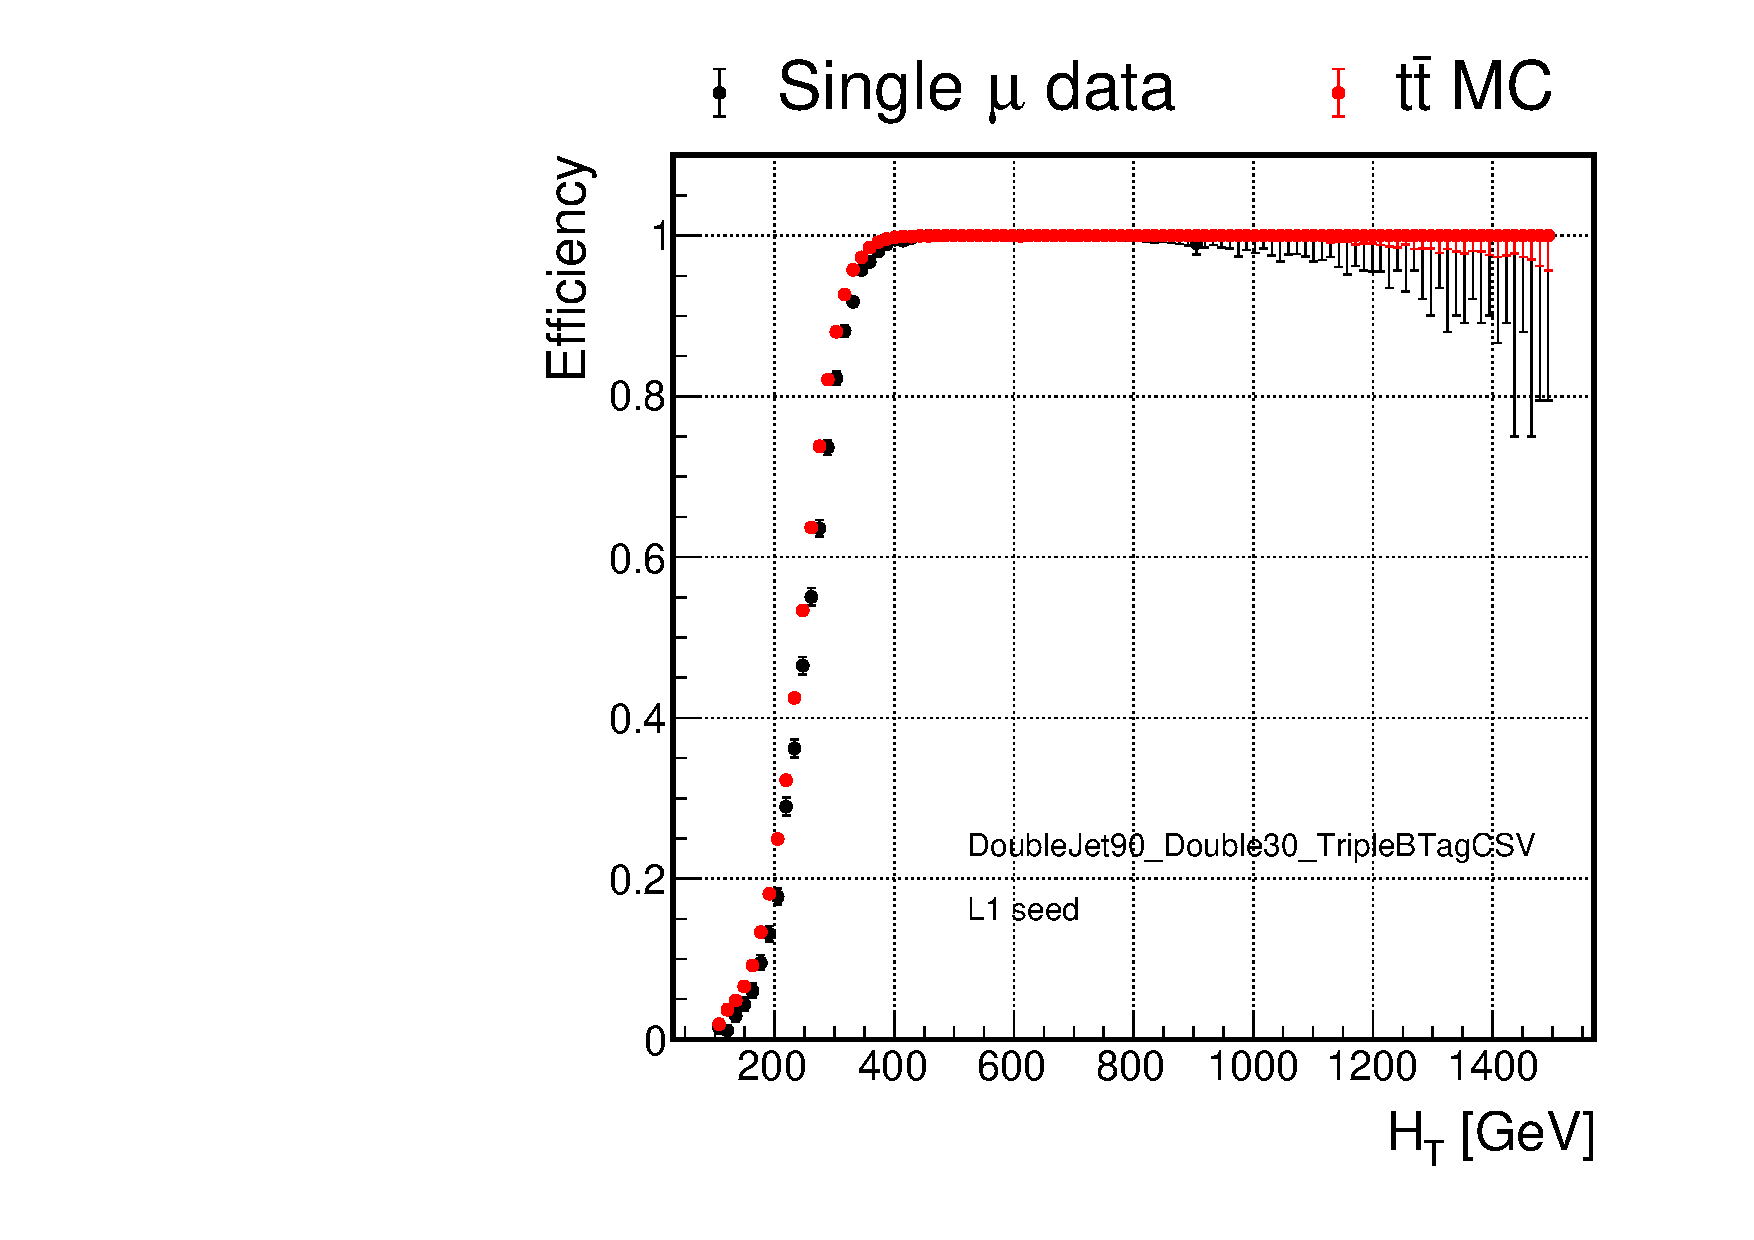
\includegraphics[width=0.4\textwidth]{Figures/AnalysisStrategy/triggereff/plots_2016/Double90Quad30_Efficiency_L1filterHT.pdf}}
\subfloat{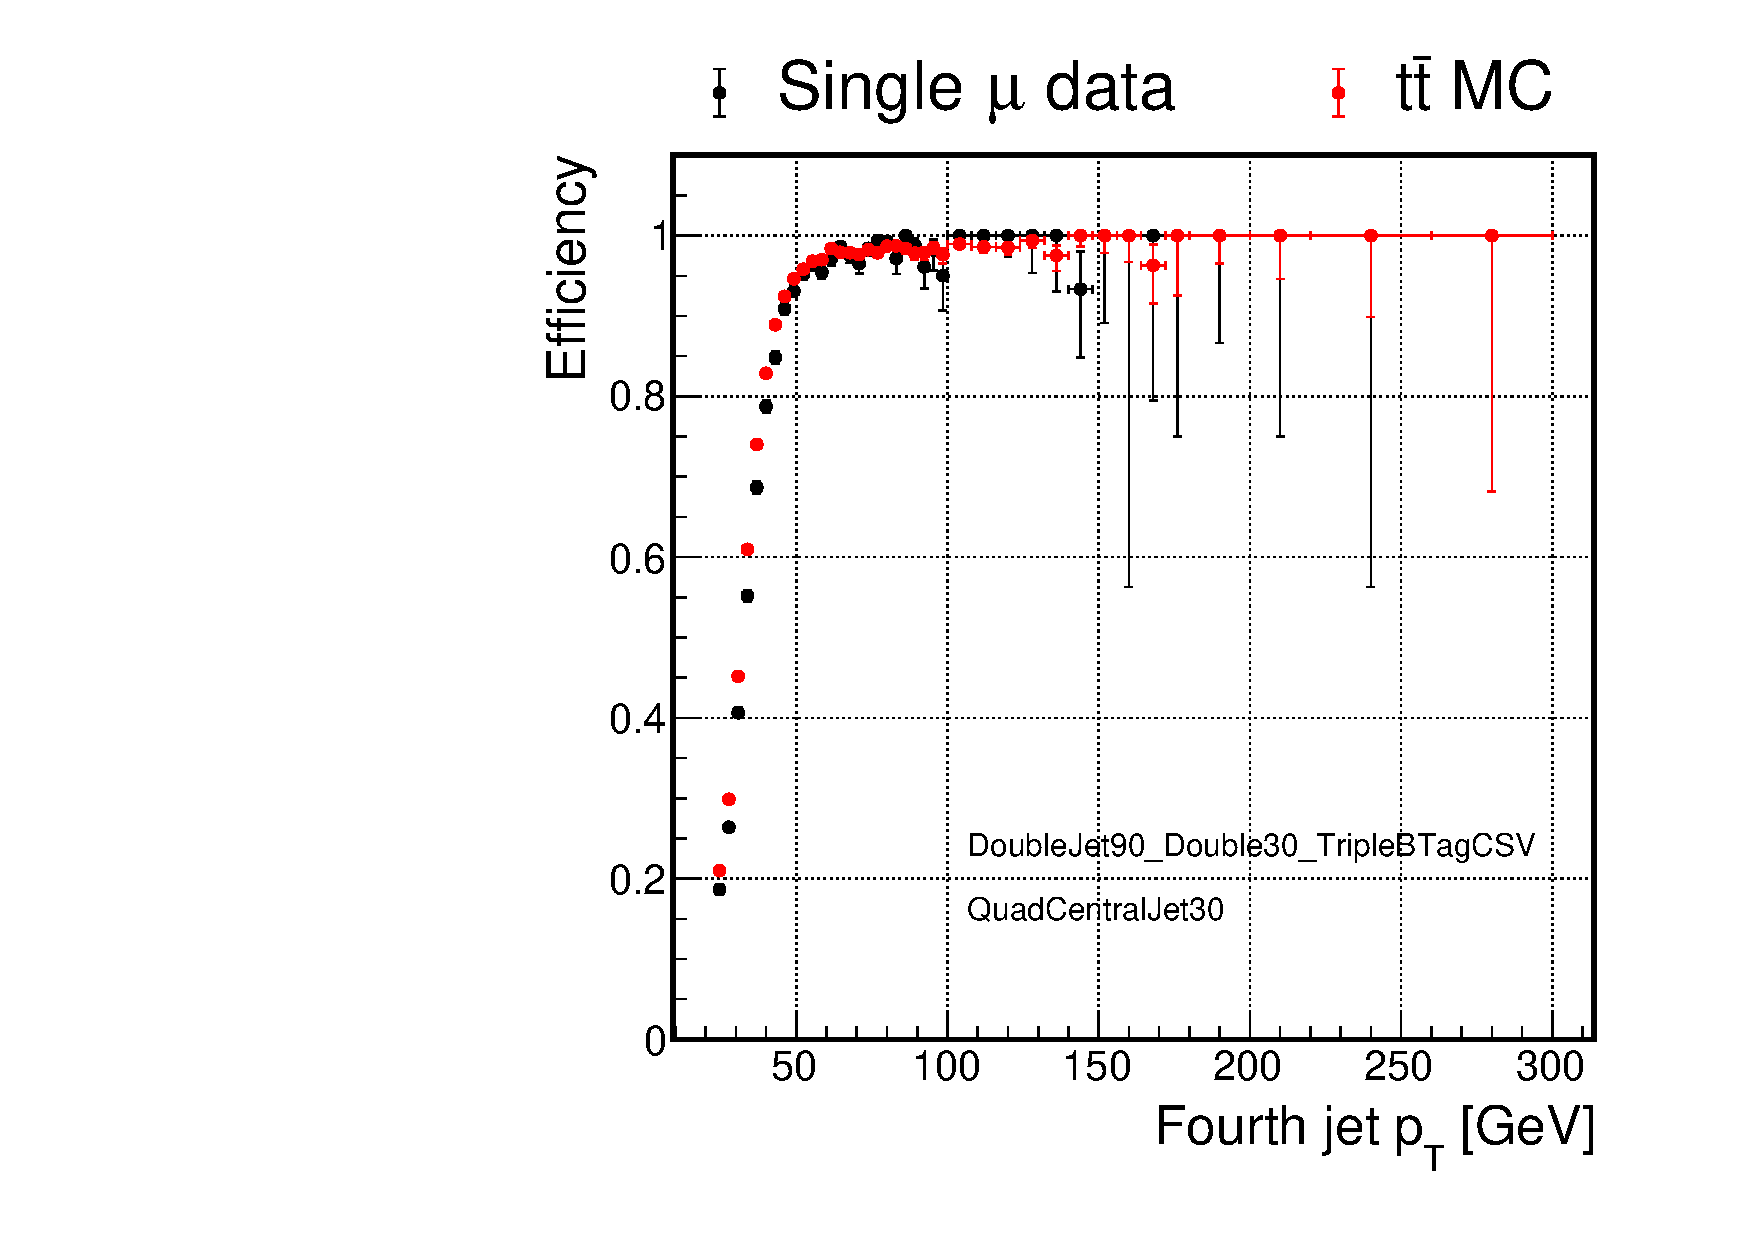
\includegraphics[width=0.4\textwidth]{Figures/AnalysisStrategy/triggereff/plots_2016/Double90Quad30_Efficiency_QuadCentralJet30.pdf}}\\
\subfloat{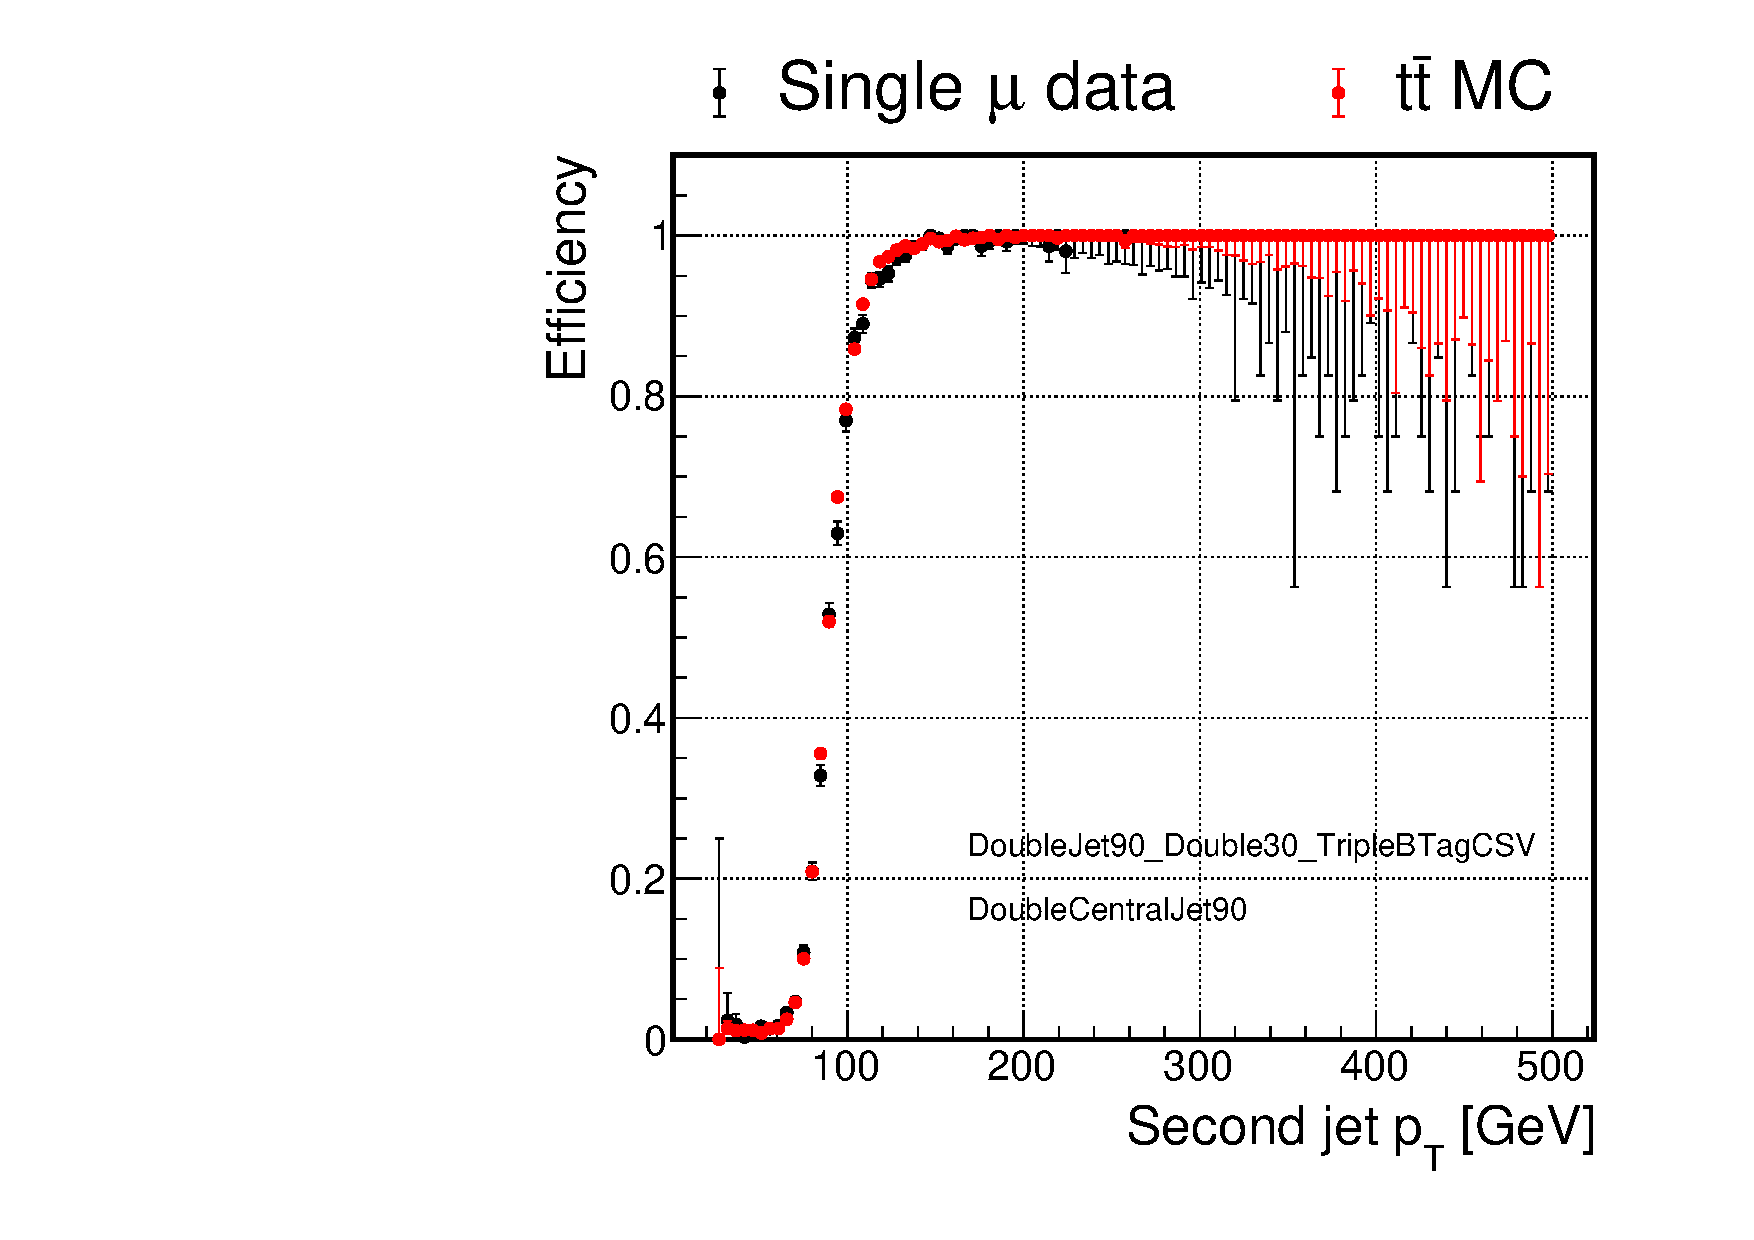
\includegraphics[width=0.4\textwidth]{Figures/AnalysisStrategy/triggereff/plots_2016/Double90Quad30_Efficiency_DoubleCentralJet90.pdf}}
\subfloat{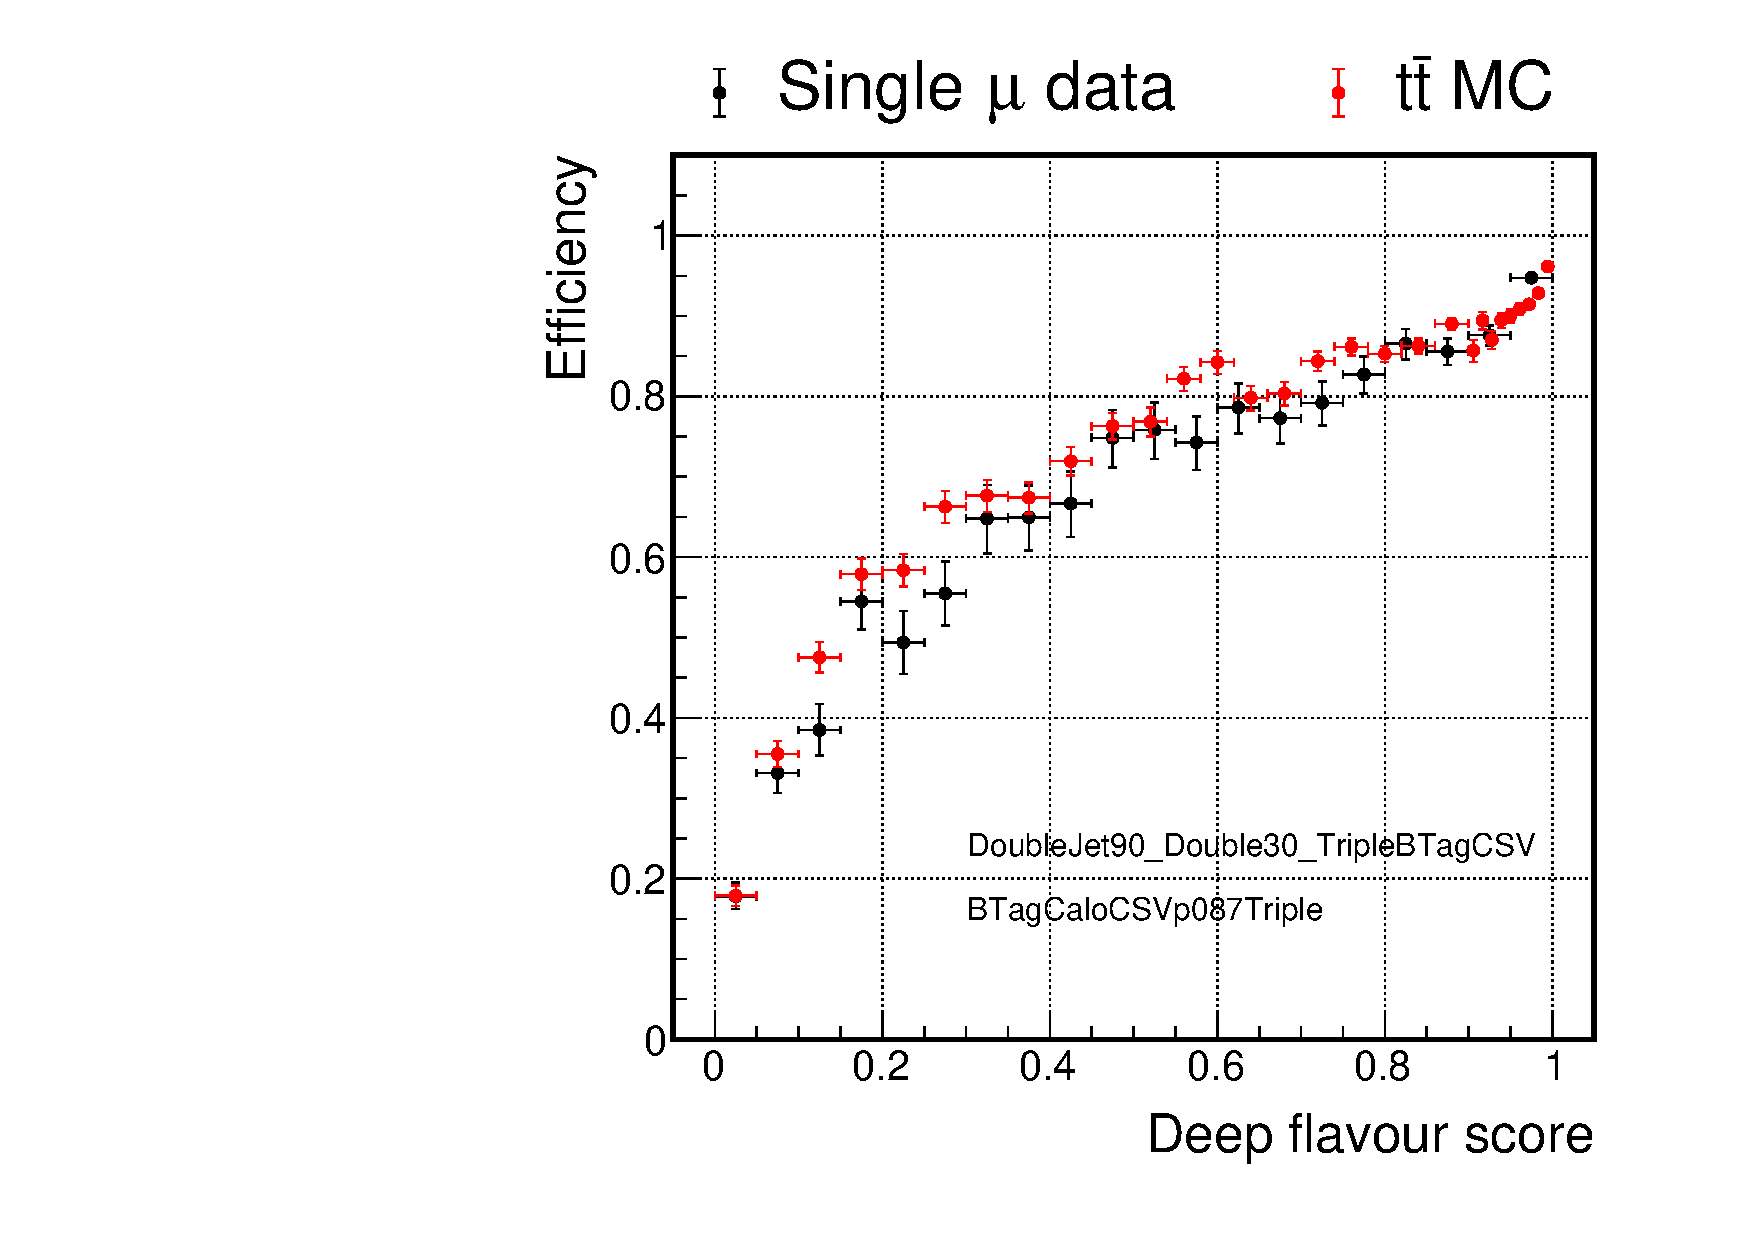
\includegraphics[width=0.4\textwidth]{Figures/AnalysisStrategy/triggereff/plots_2016/Double90Quad30_Efficiency_BTagCaloCSVp087Triple.pdf}}\\
\subfloat{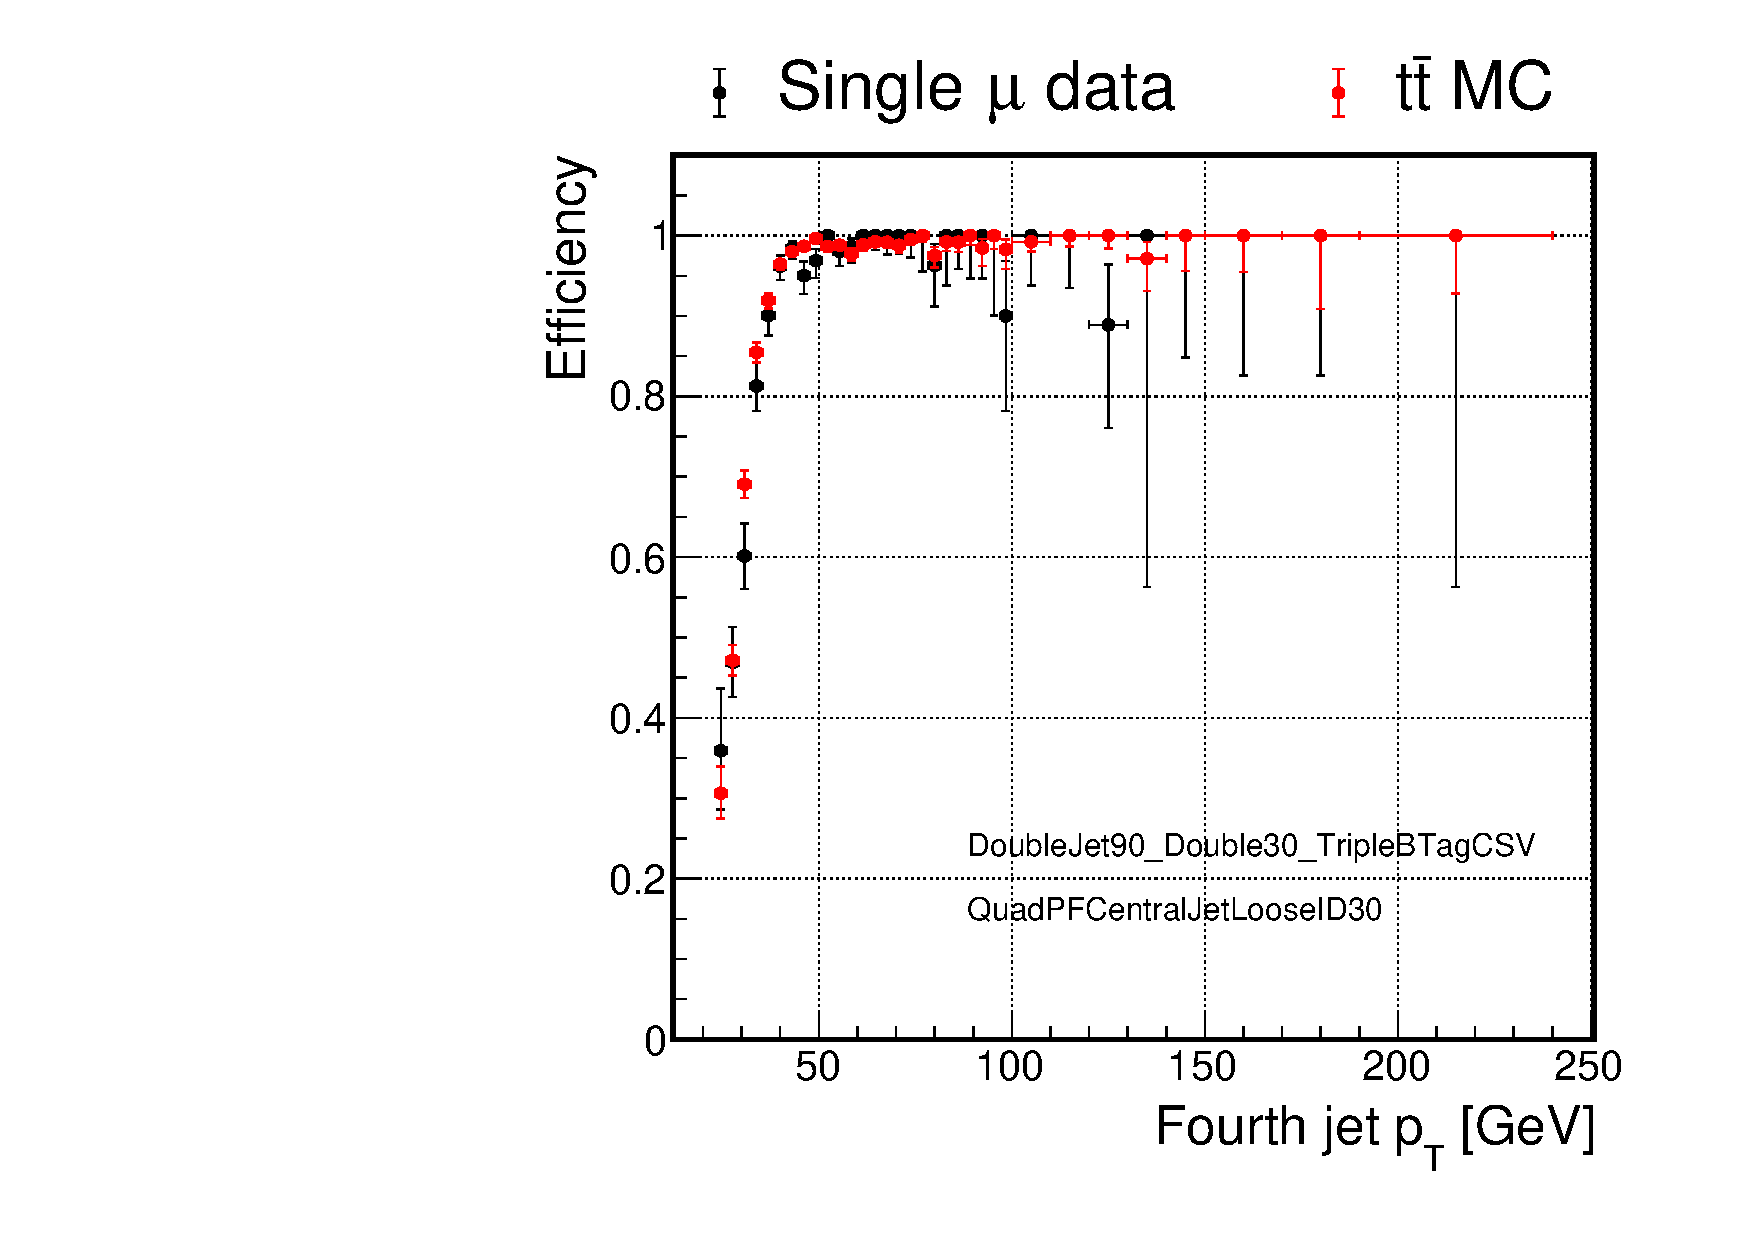
\includegraphics[width=0.4\textwidth]{Figures/AnalysisStrategy/triggereff/plots_2016/Double90Quad30_Efficiency_QuadPFCentralJetLooseID30.pdf}}
\subfloat{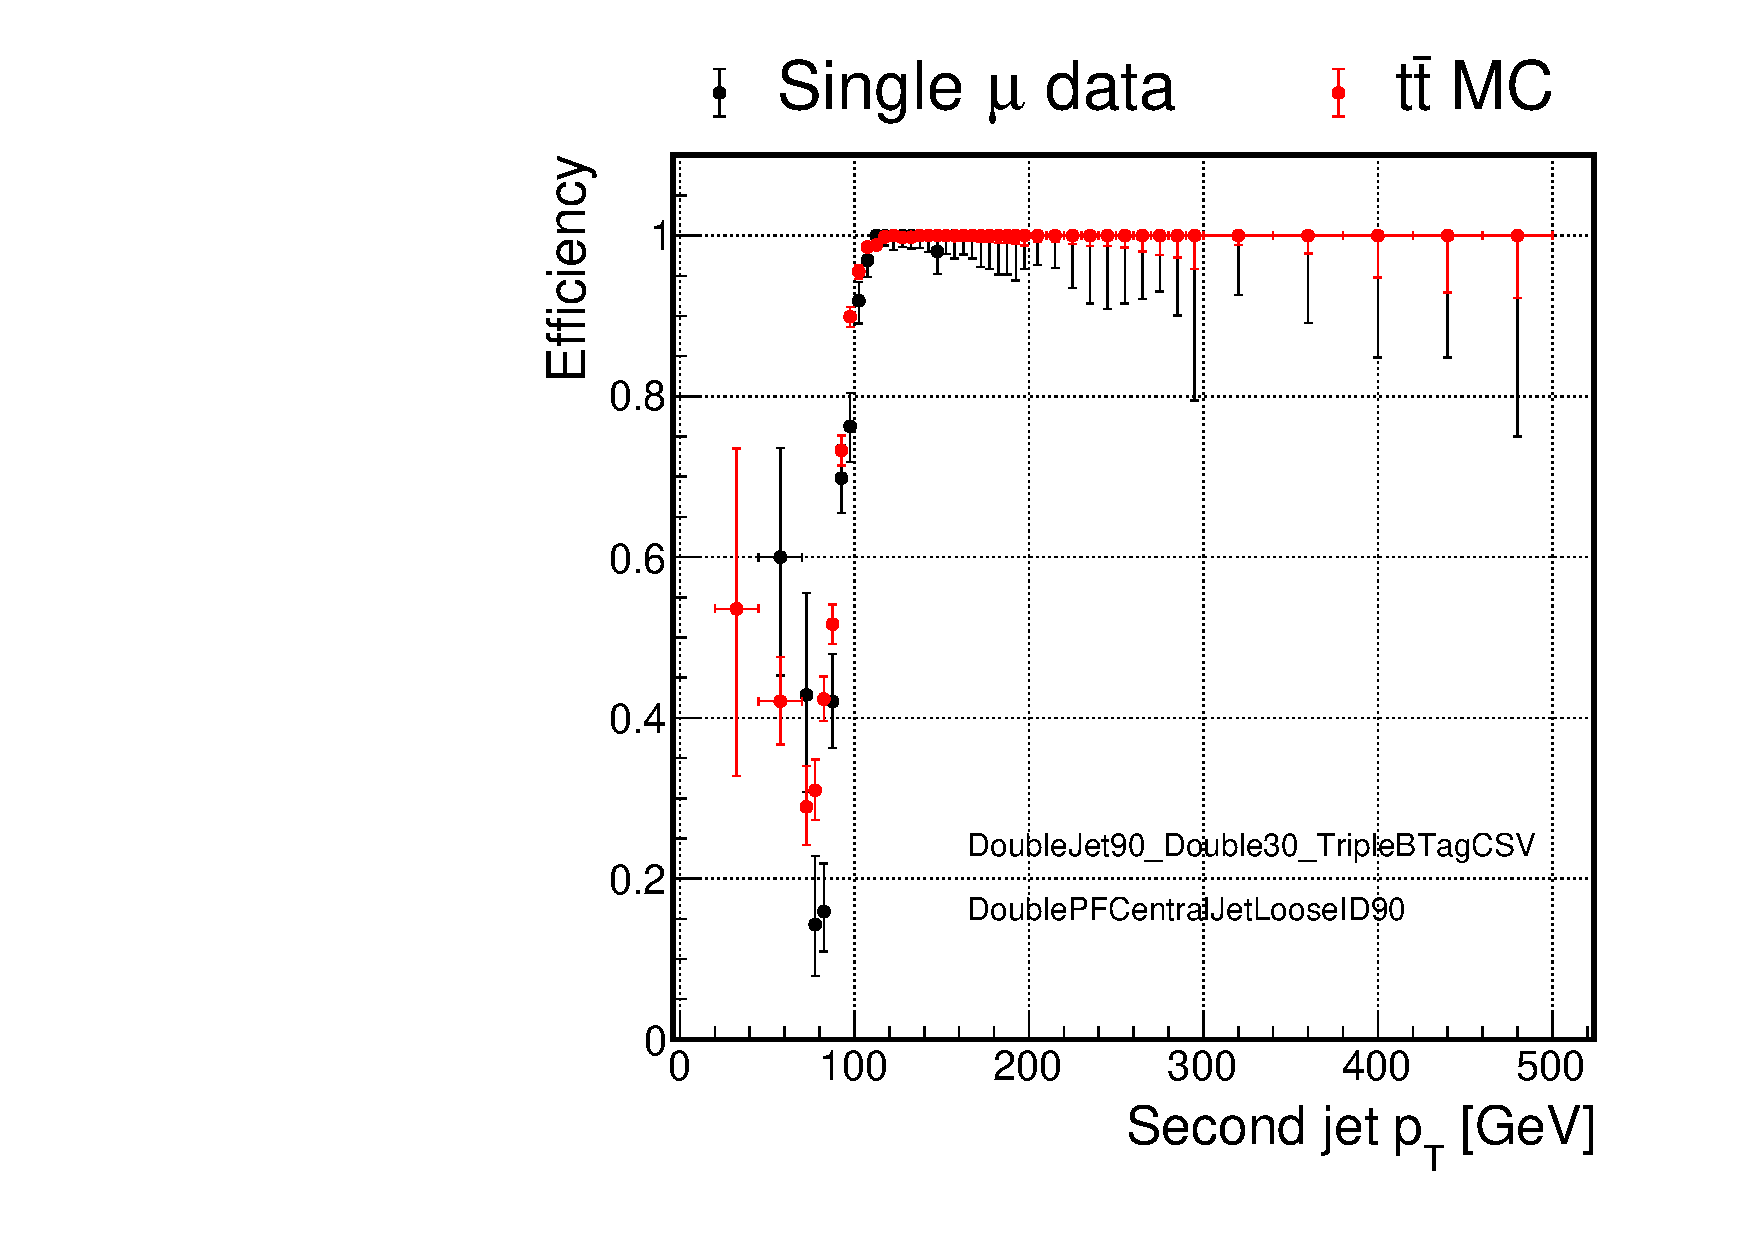
\includegraphics[width=0.4\textwidth]{Figures/AnalysisStrategy/triggereff/plots_2016/Double90Quad30_Efficiency_DoublePFCentralJetLooseID90.pdf}}
\caption[Efficiency measured in single muon data and $\ttbar$ MC for filters of HLT\_DoubleJet90\_Double30\_TripleBTagCSV path in 2016]{Efficiency measured in single muon data (black) and $\ttbar$ MC (red) for filters of HLT\_DoubleJet90\_Double30\_TripleBTagCSV, corresponding to the 2016 dataset.}
\label{trigger:fig:filterEfficiency2016DoubleOverlap}
\end{figure}

\begin{figure}[p]
\centering
\subfloat{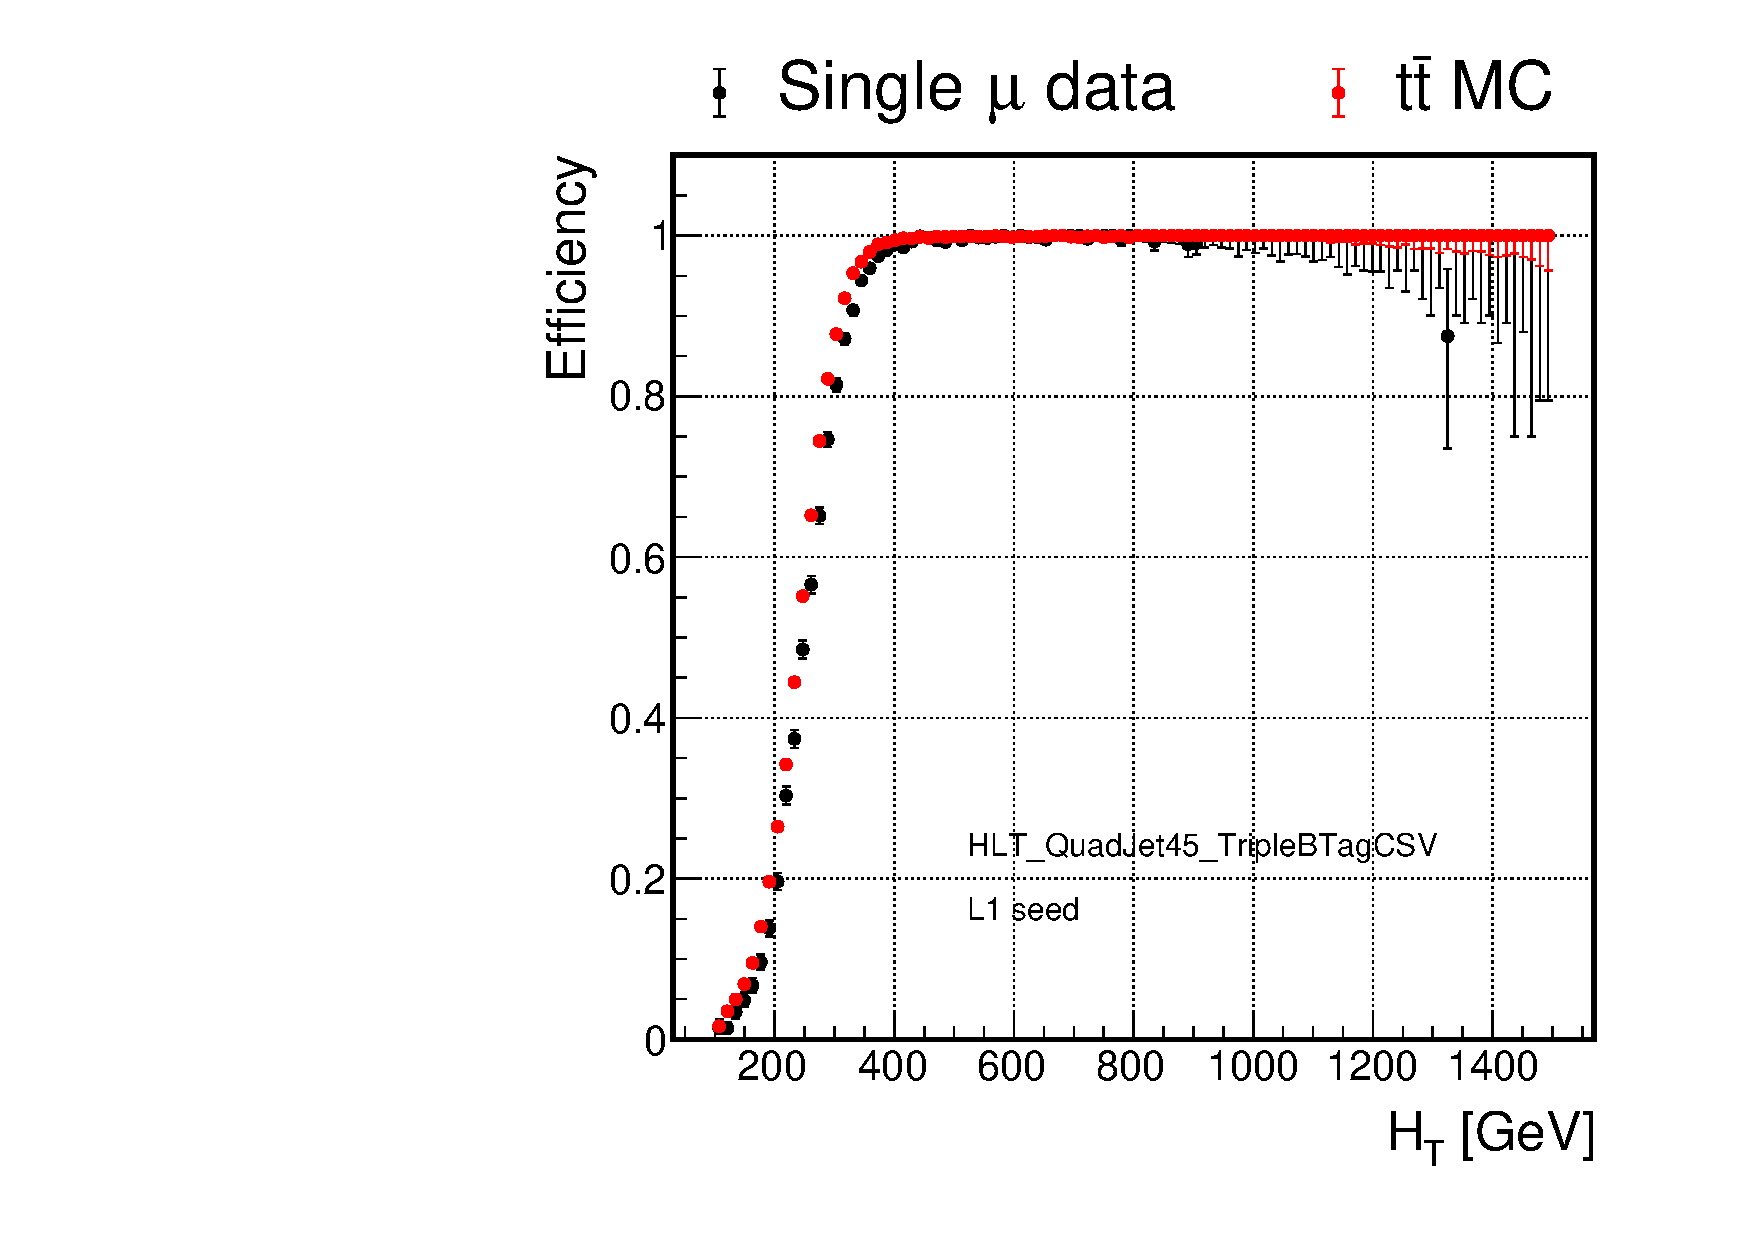
\includegraphics[width=0.4\textwidth]{Figures/AnalysisStrategy/triggereff/plots_2016/Quad45_Efficiency_L1filterHT.pdf}}
\subfloat{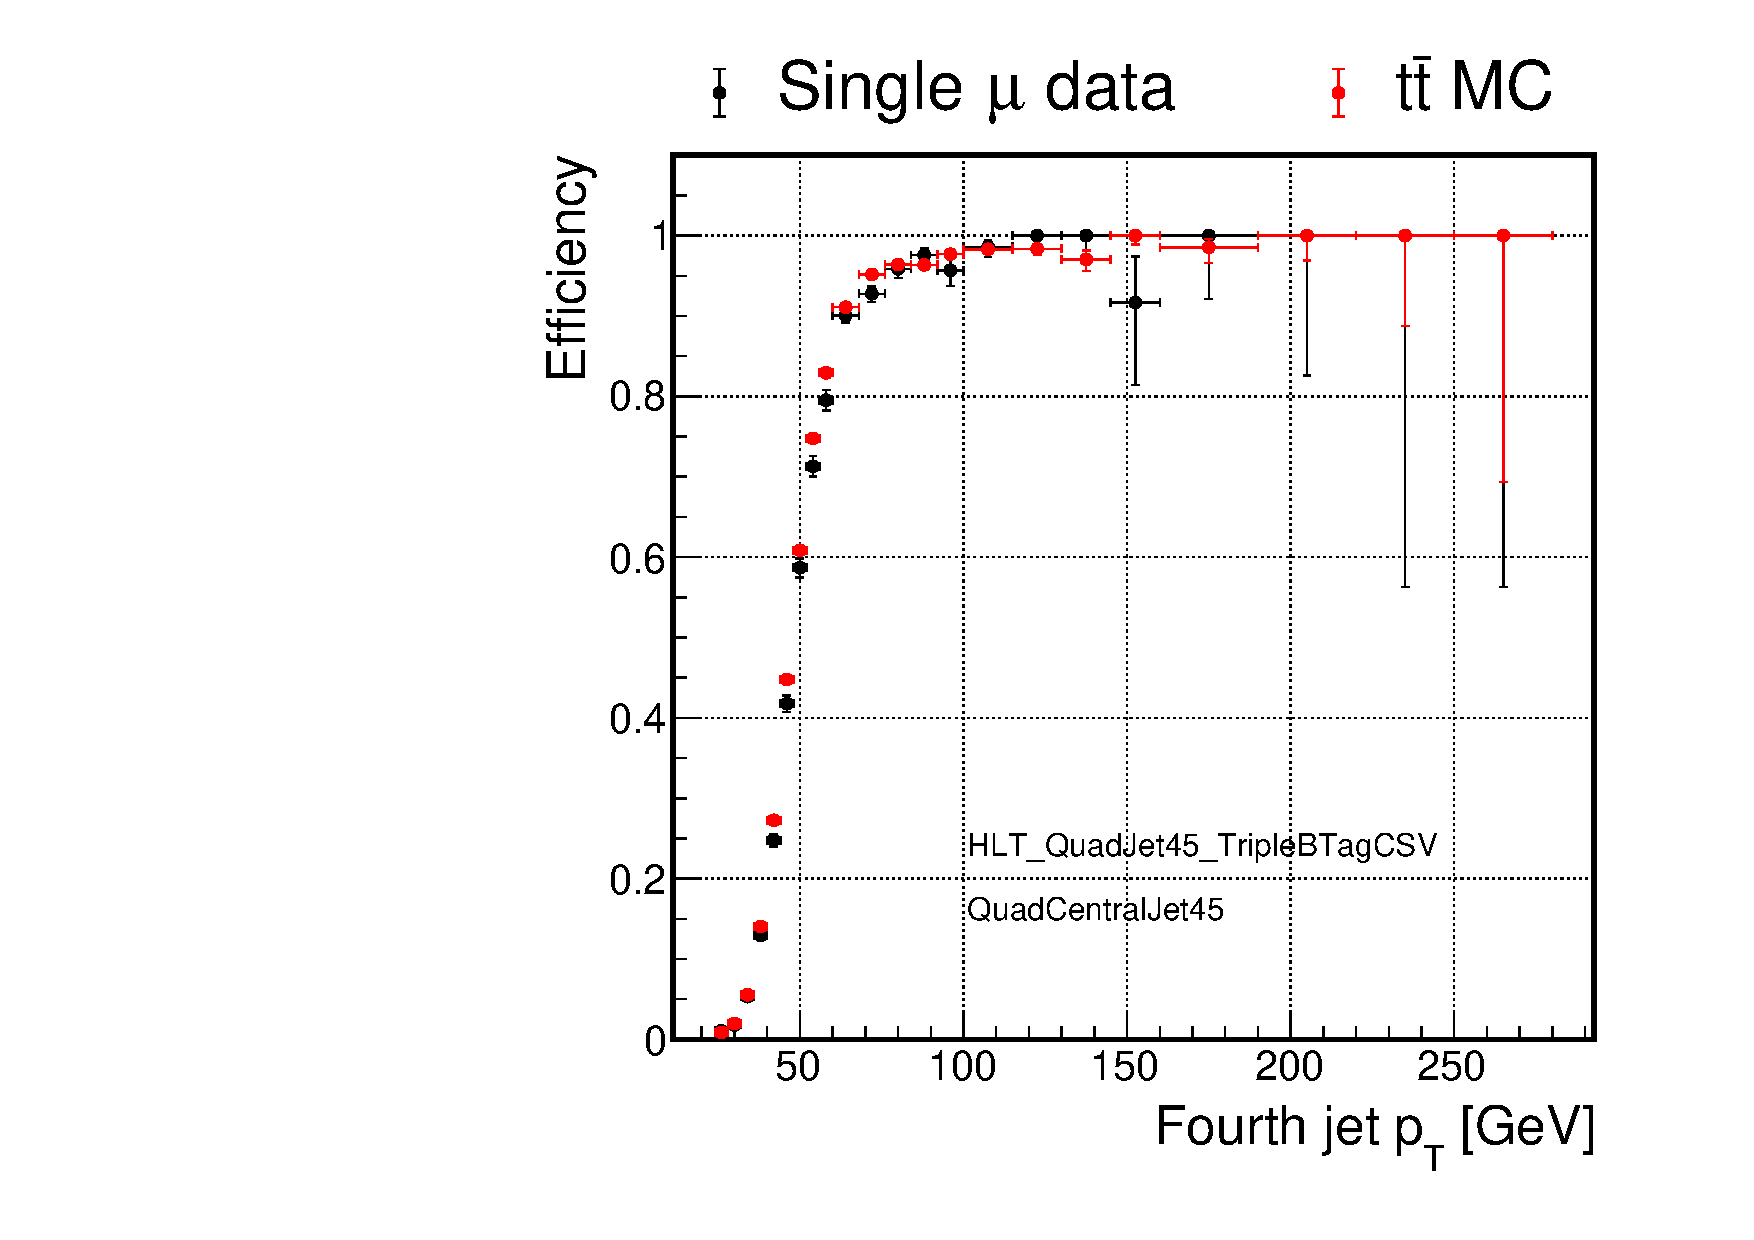
\includegraphics[width=0.4\textwidth]{Figures/AnalysisStrategy/triggereff/plots_2016/Quad45_Efficiency_QuadCentralJet45.pdf}}\\
\subfloat{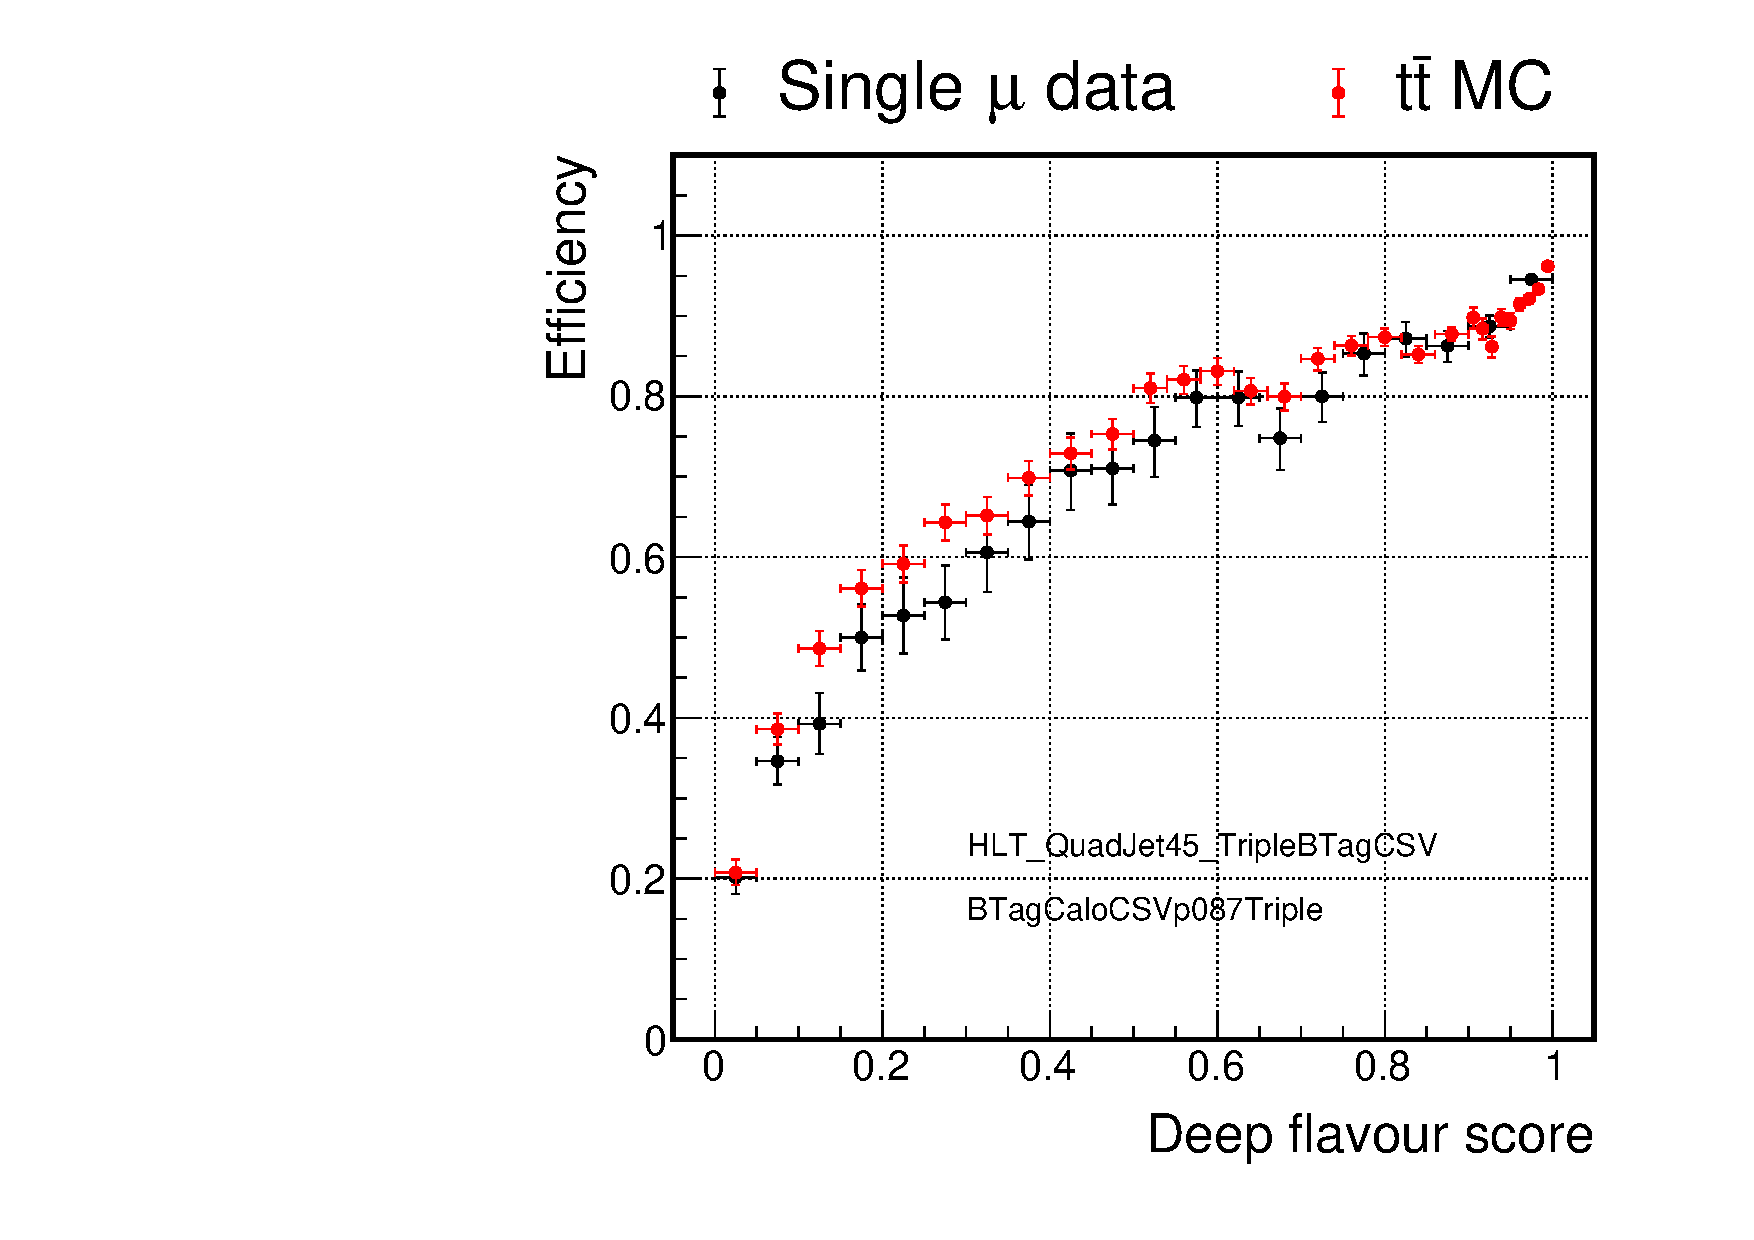
\includegraphics[width=0.4\textwidth]{Figures/AnalysisStrategy/triggereff/plots_2016/Quad45_Efficiency_BTagCaloCSVp087Triple.pdf}}
\subfloat{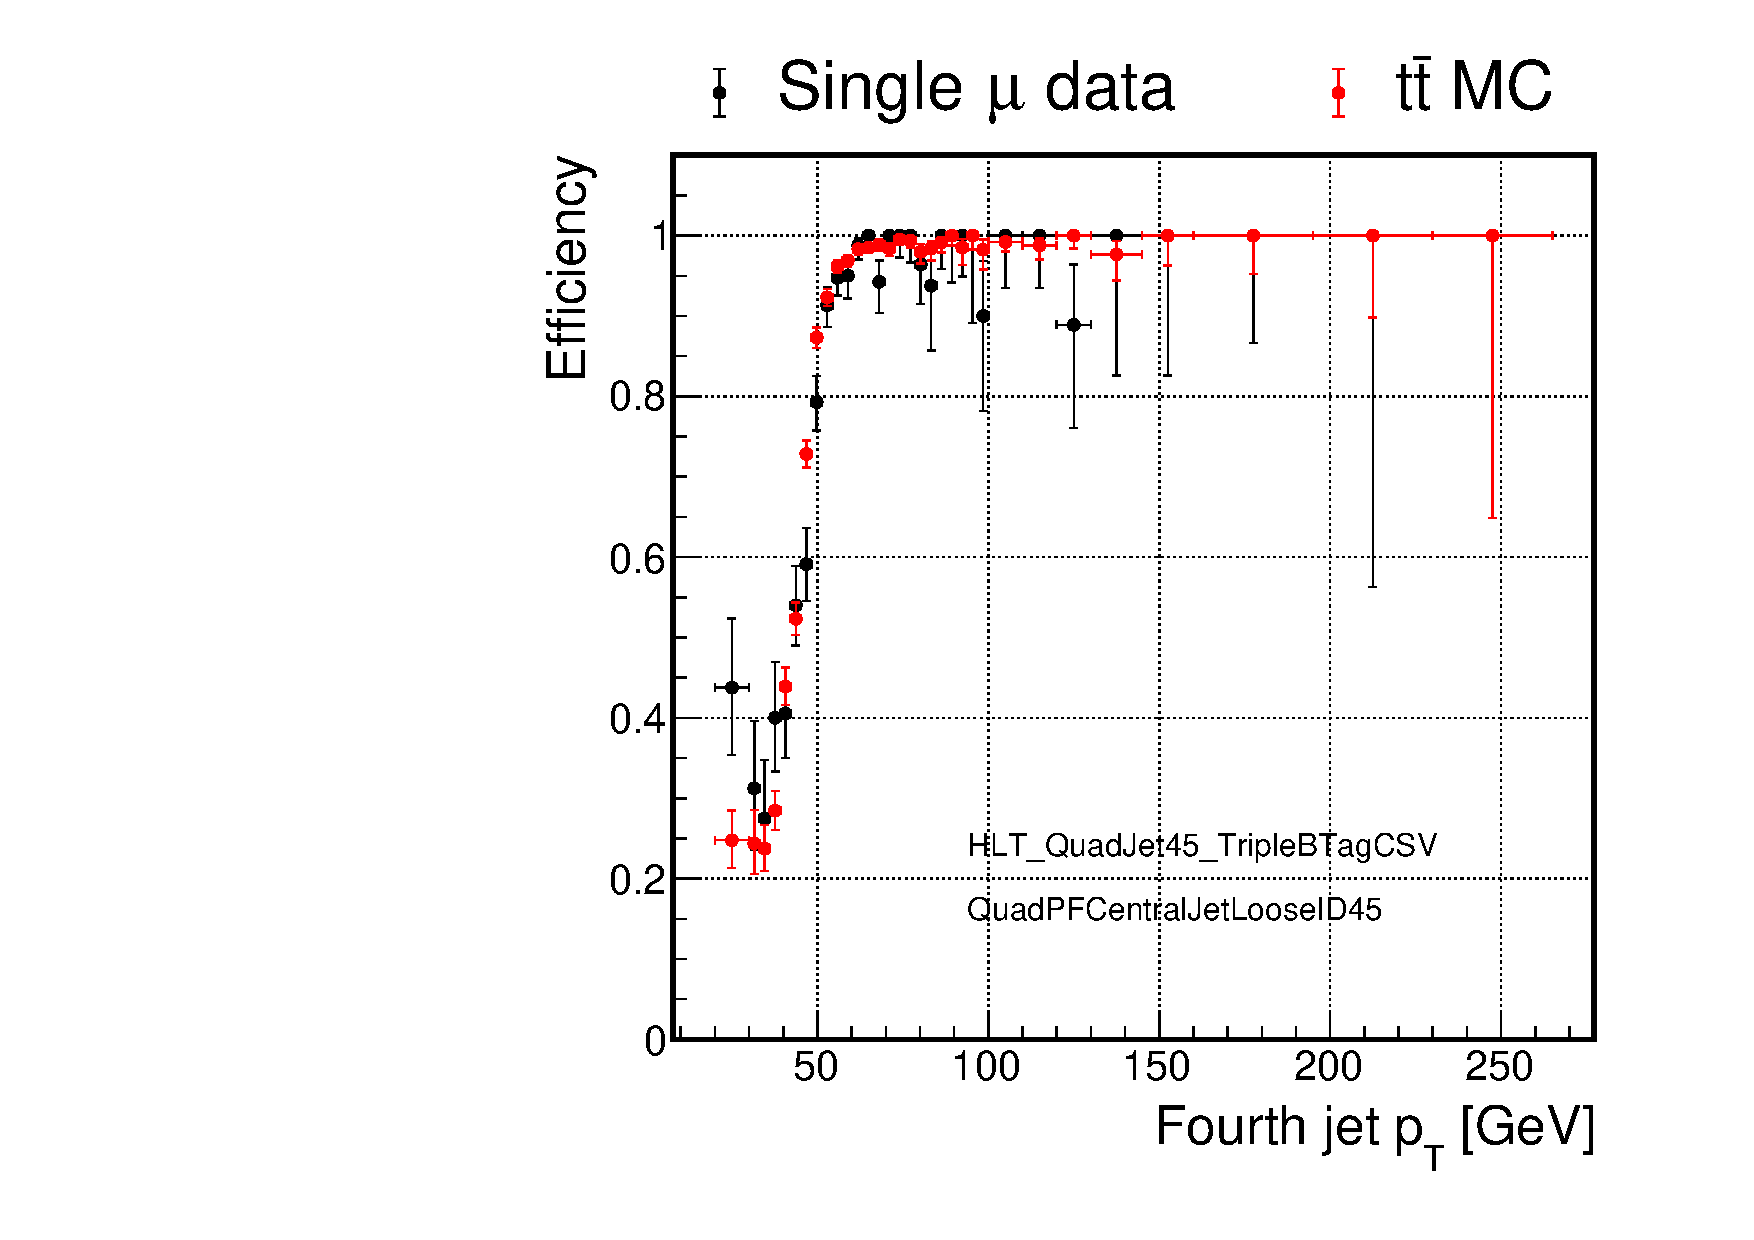
\includegraphics[width=0.4\textwidth]{Figures/AnalysisStrategy/triggereff/plots_2016/Quad45_Efficiency_QuadPFCentralJetLooseID45.pdf}}
\caption[Efficiency measured in single muon data and $\ttbar$ MC for filters of HLT\_QuadJet45\_TripleBTagCSV path in 2016]{Efficiency measured in single muon data (black) and $\ttbar$ MC (red) for filters of HLT\_QuadJet45\_TripleBTagCSV, corresponding to the 2016 dataset.}
\label{trigger:fig:filterEfficiency2016QuadOverlap}
\end{figure}

\begin{figure}[p]
\centering
\subfloat{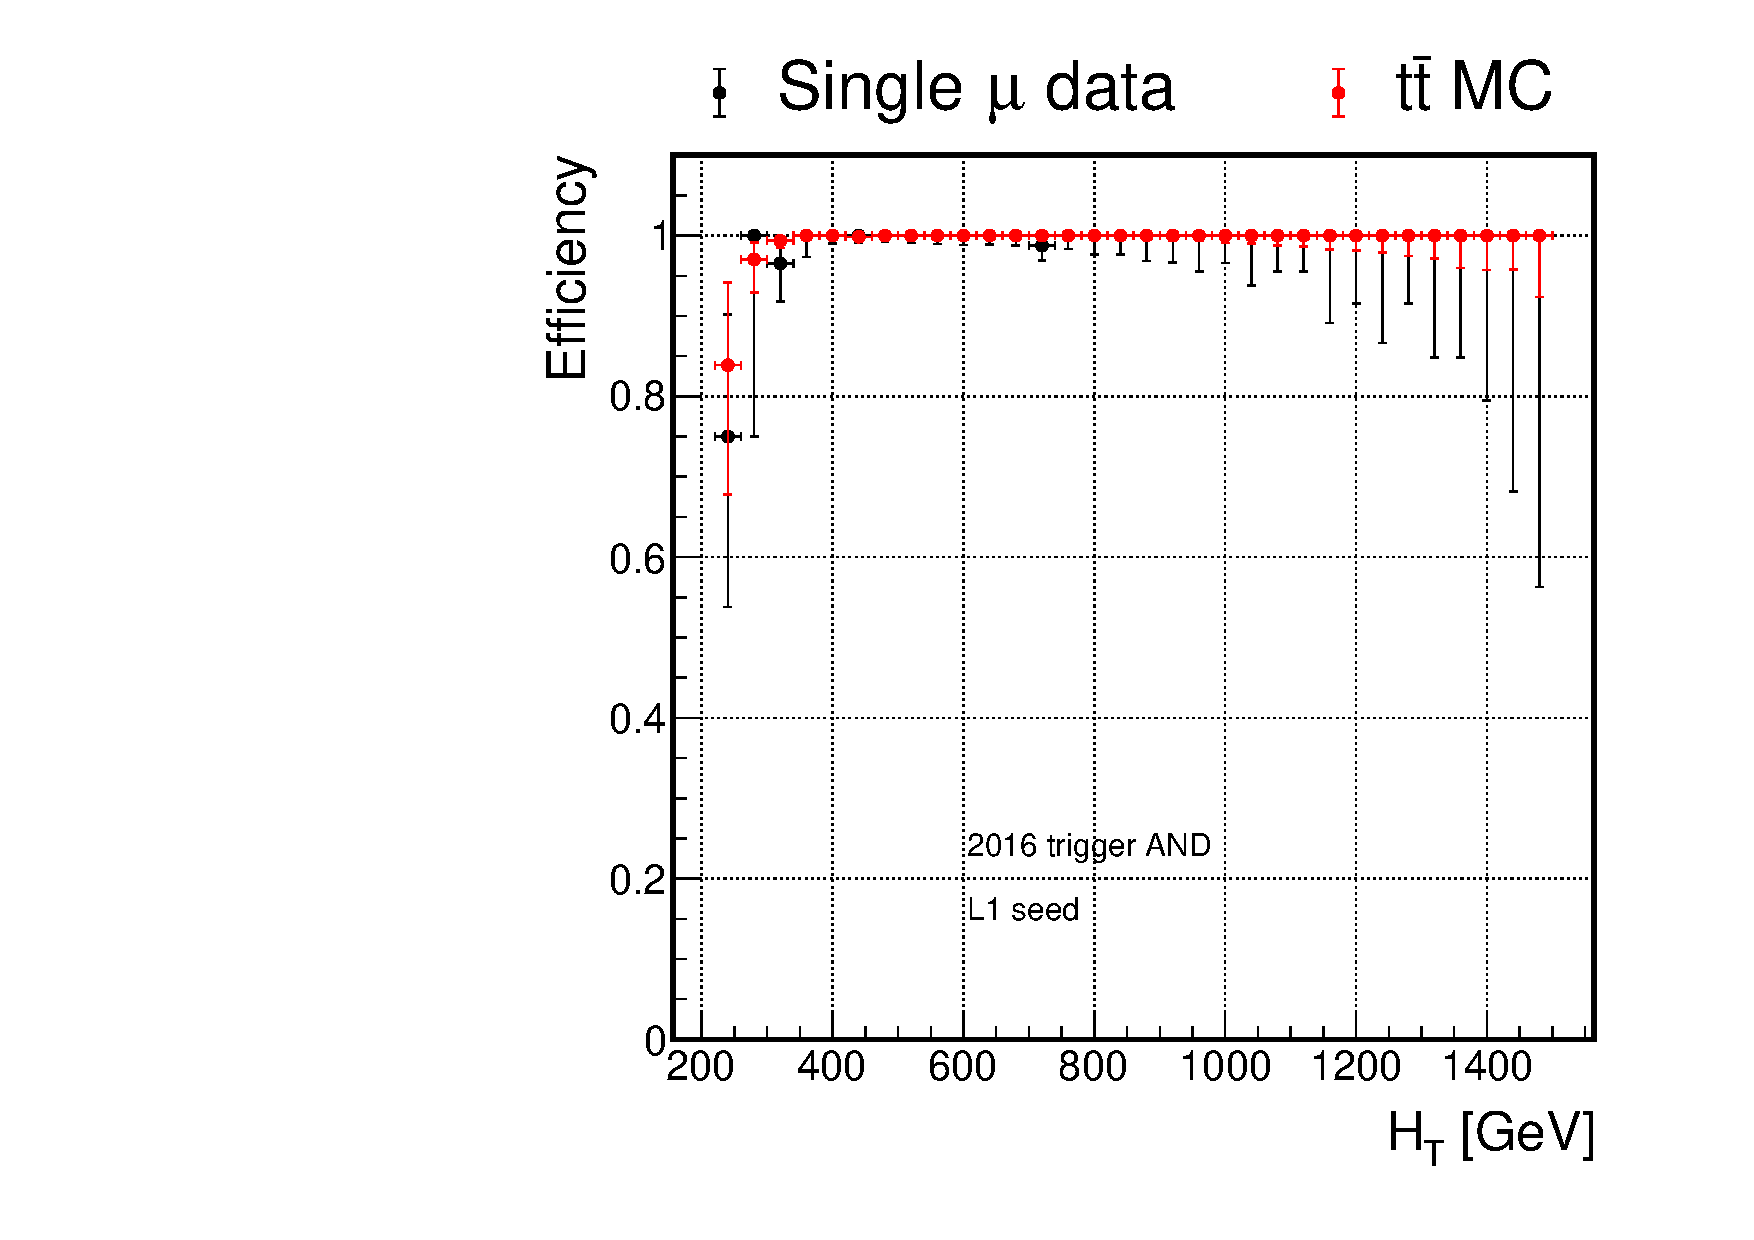
\includegraphics[width=0.4\textwidth]{Figures/AnalysisStrategy/triggereff/plots_2016/And_Efficiency_L1filterQuad45HT.pdf}}
\subfloat{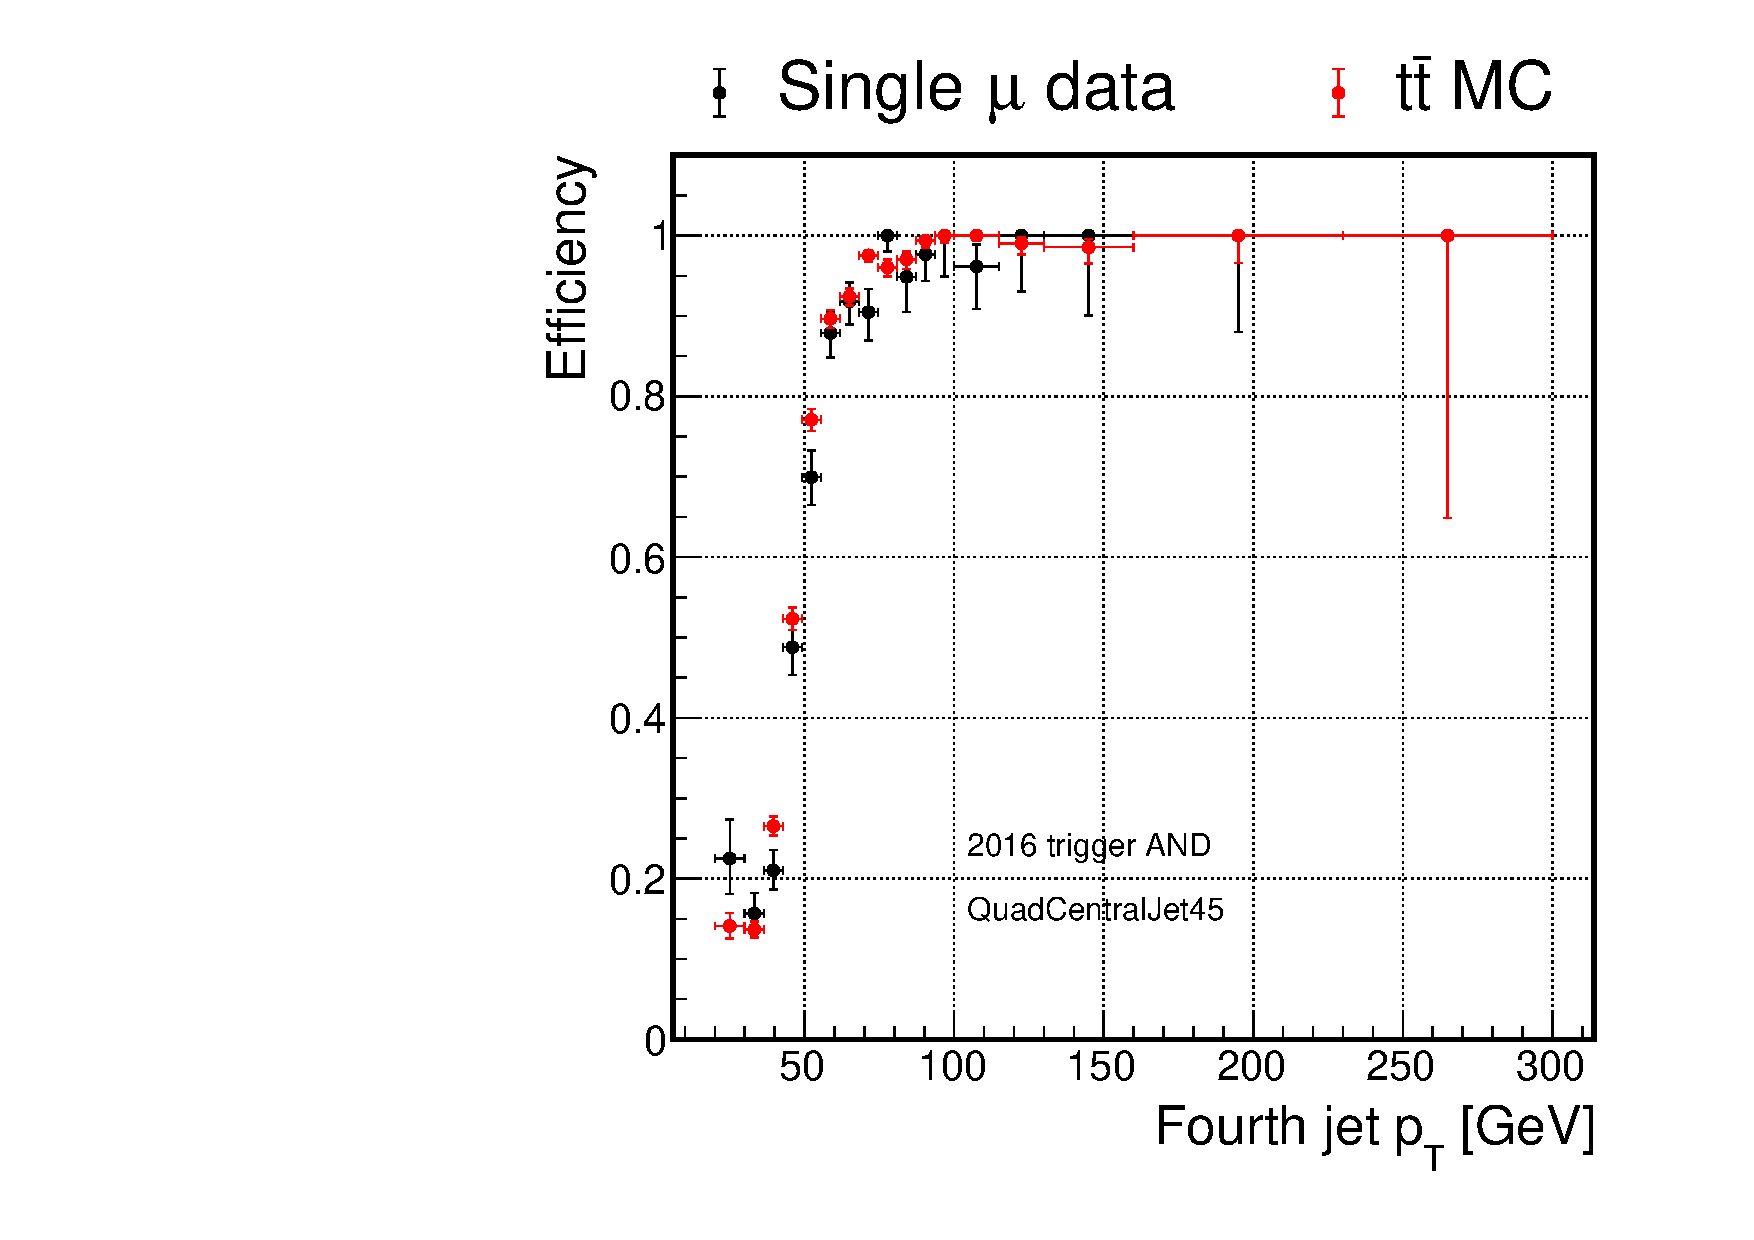
\includegraphics[width=0.4\textwidth]{Figures/AnalysisStrategy/triggereff/plots_2016/And_Efficiency_QuadCentralJet45.pdf}}\\
\subfloat{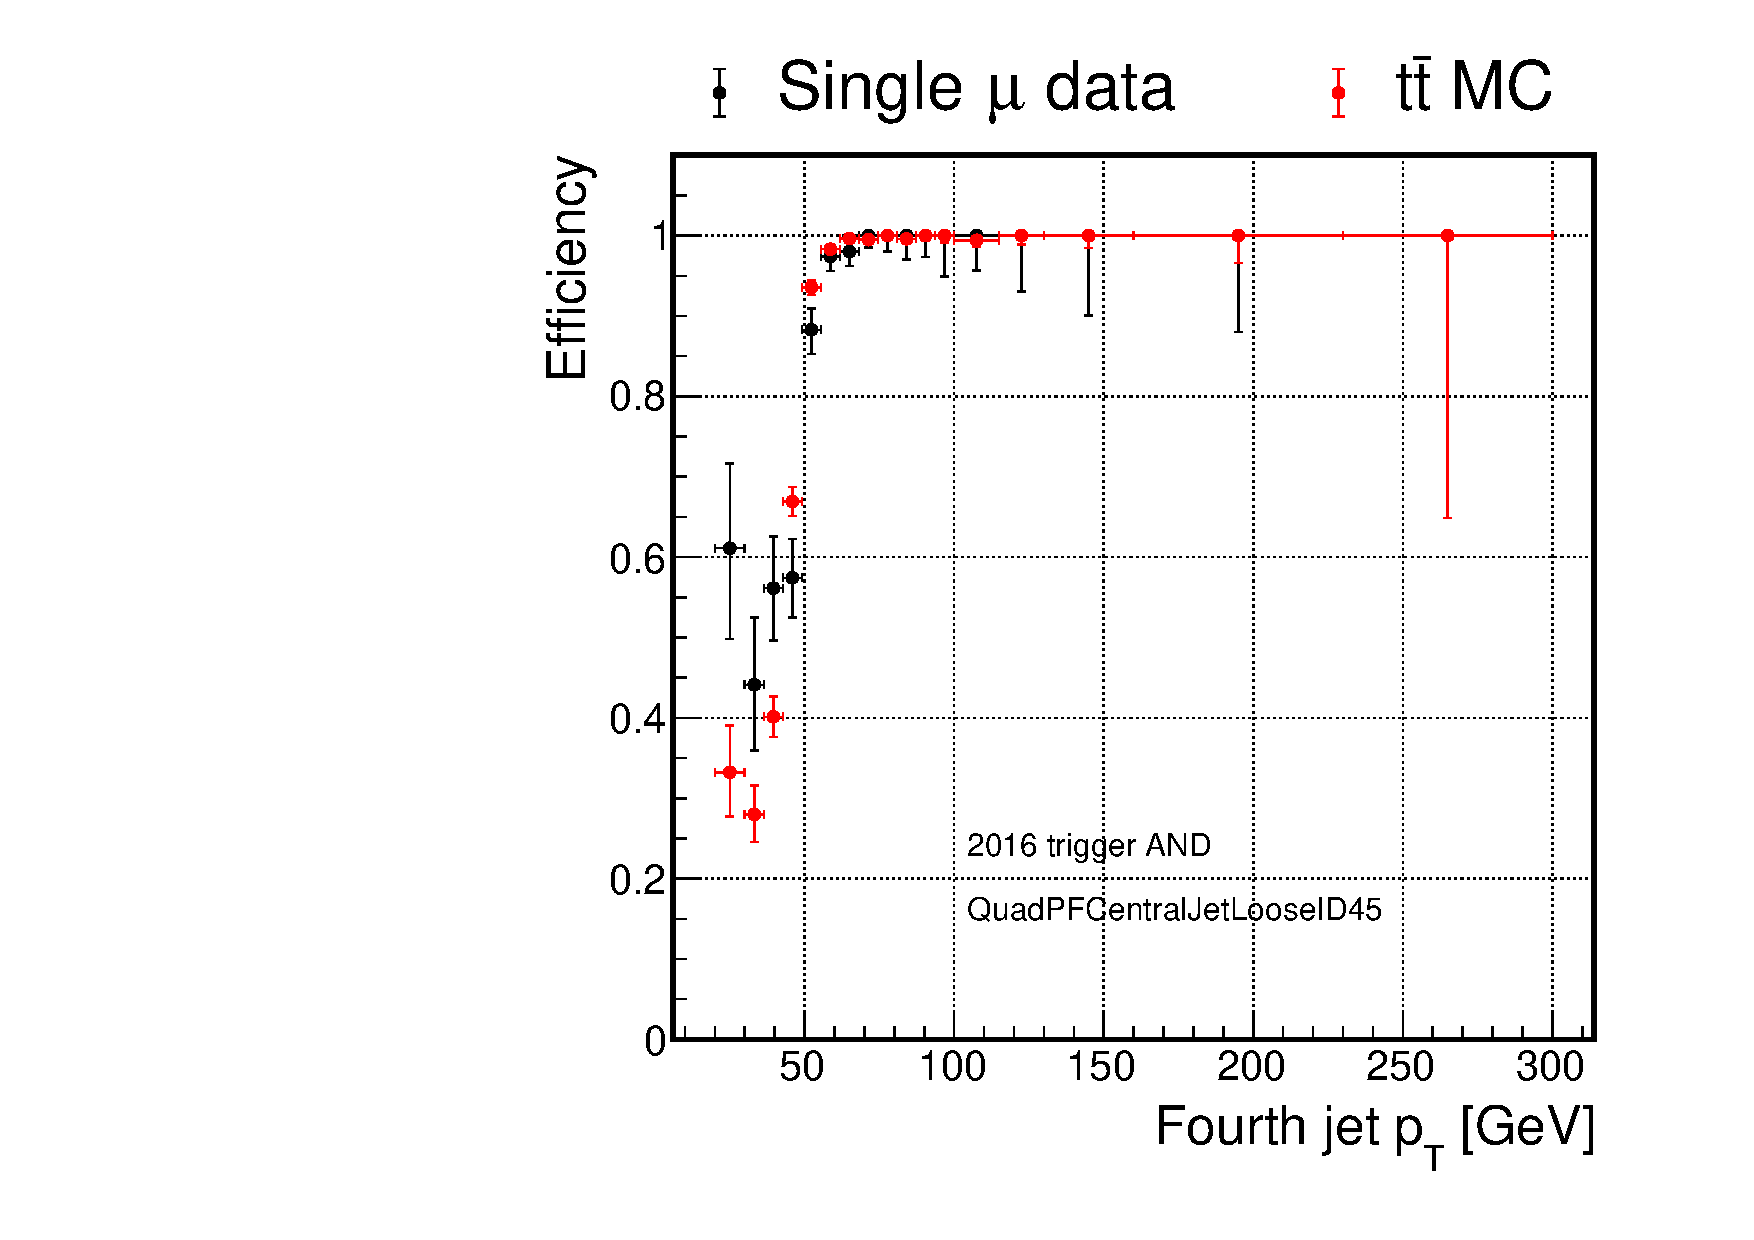
\includegraphics[width=0.4\textwidth]{Figures/AnalysisStrategy/triggereff/plots_2016/And_Efficiency_QuadPFCentralJetLooseID45.pdf}}
\caption[Efficiency measured in single muon data and $\ttbar$ MC for filters of the path overlap in 2016]{Efficiency measured in single muon data and $\ttbar$ MC for filters of HLT\_QuadJet45\_TripleBTagCSV evaluated over a sample of events passing HLT\_DoubleJet90\_Double30\_TripleBTagCSV, corresponding to the 2016 dataset.}
\label{trigger:fig:filterEfficiency2016AndOverlap}
\end{figure}

\begin{figure}[p]
\centering
\subfloat{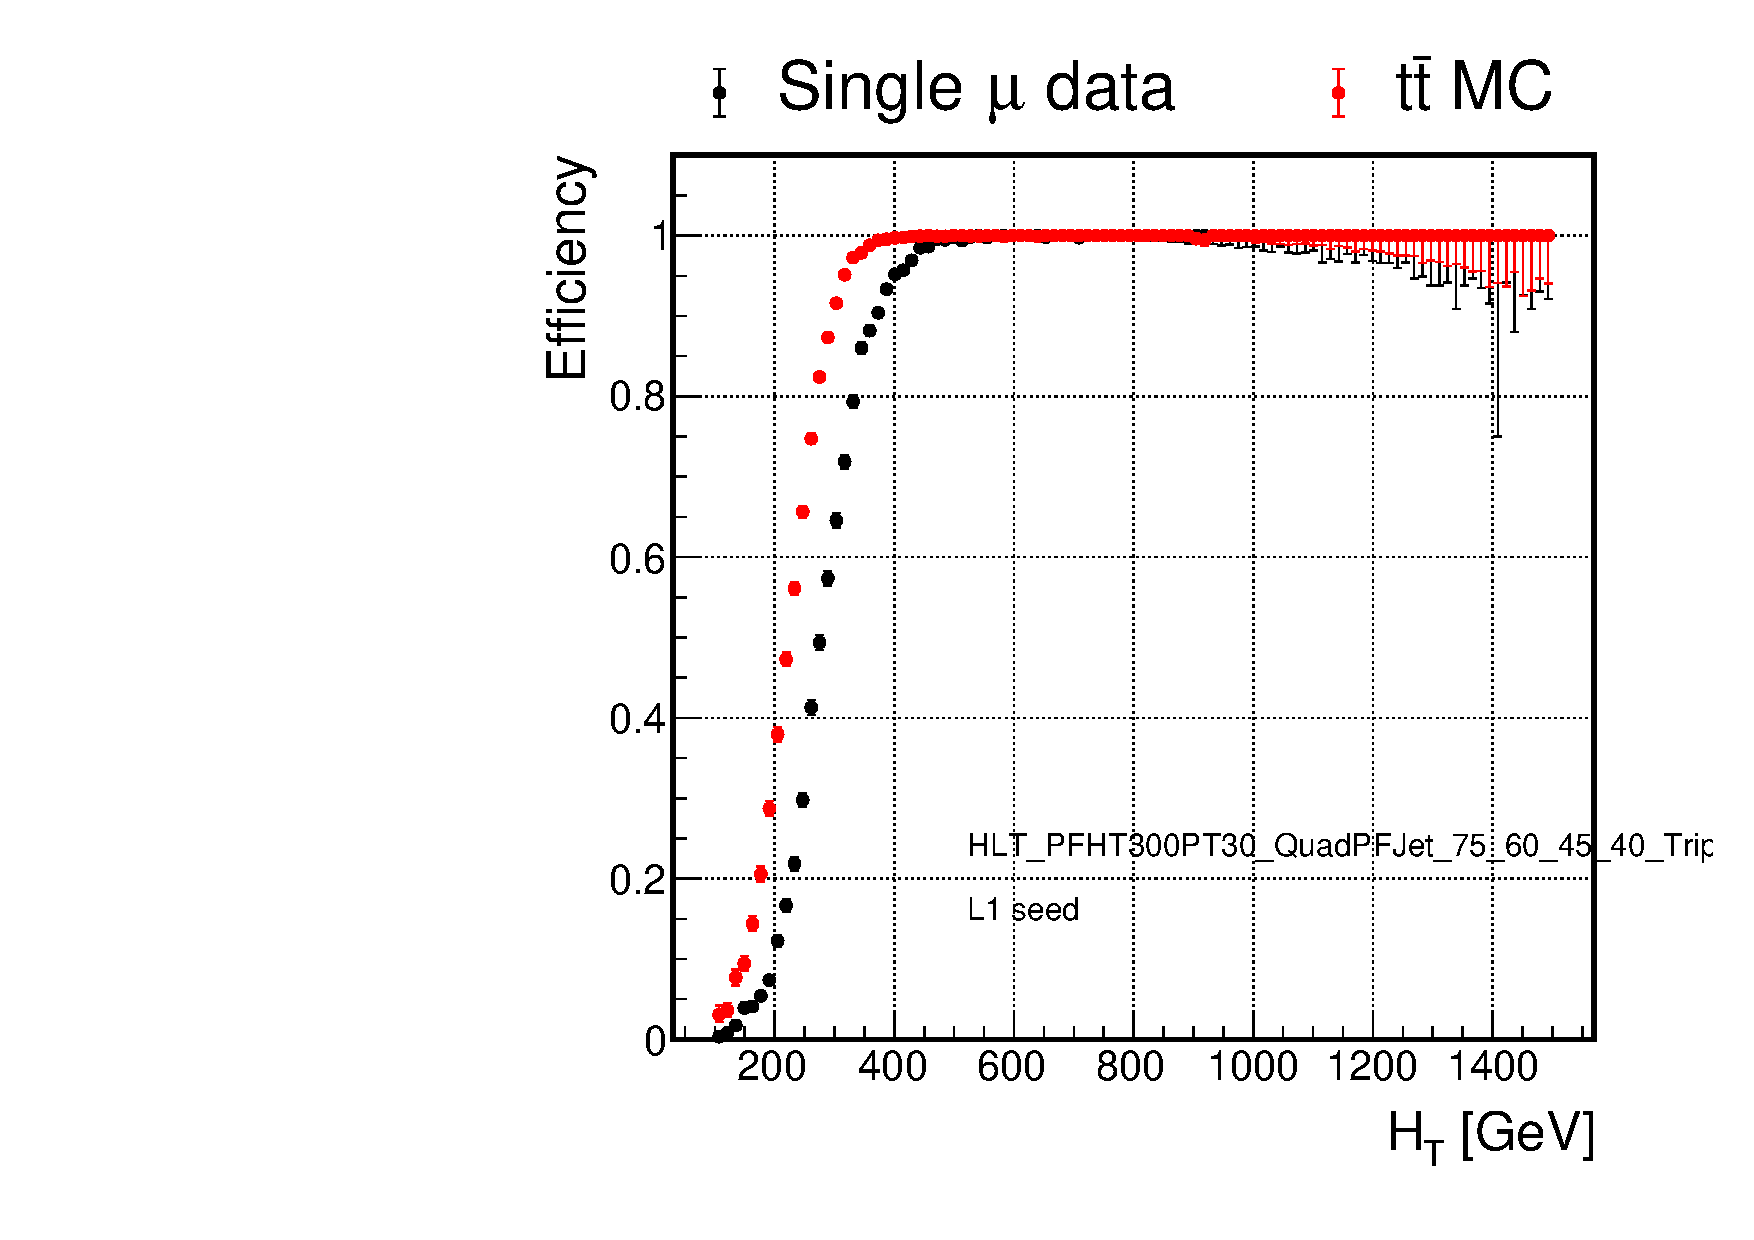
\includegraphics[width=0.3\textwidth]{Figures/AnalysisStrategy/triggereff/plots_2017/Quad_75_60_45_40_3b_Efficiency_L1filterHT.pdf}}
\subfloat{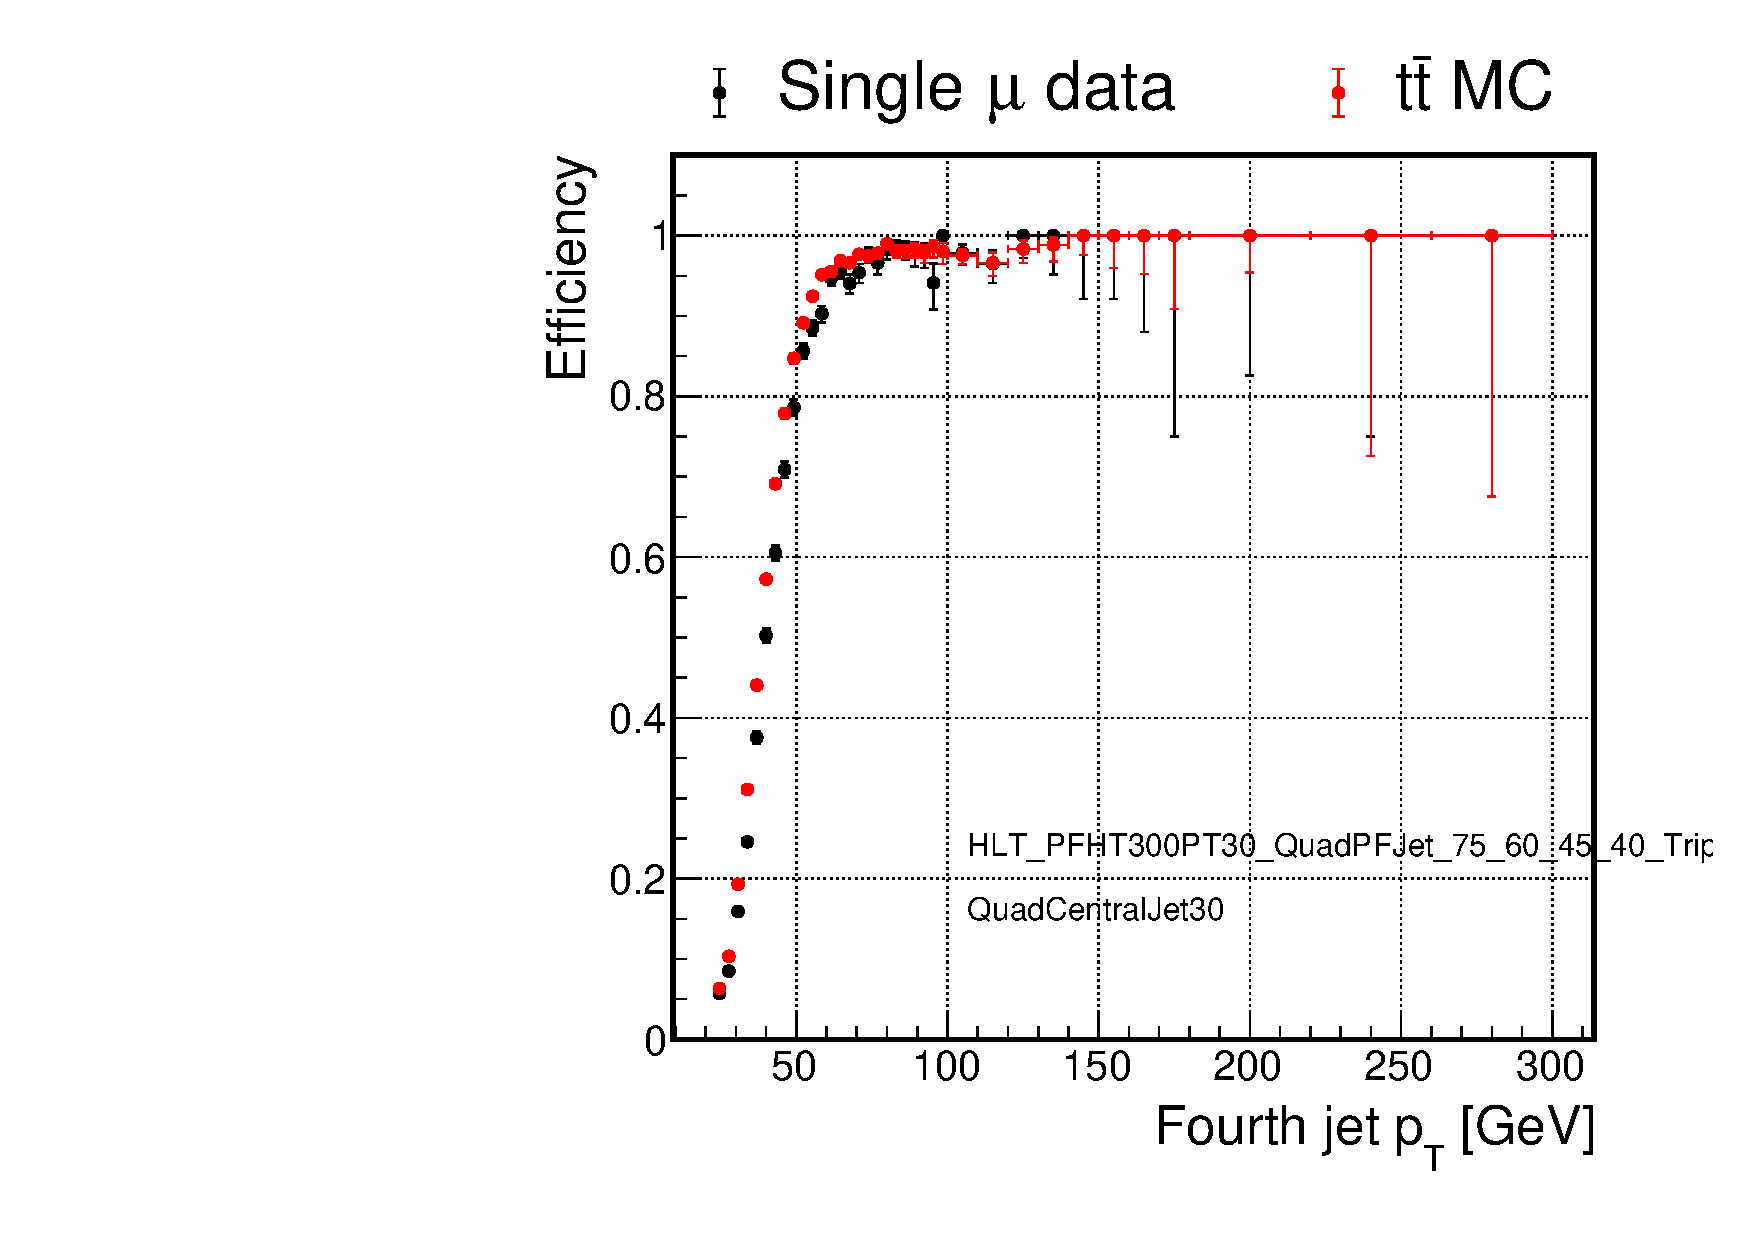
\includegraphics[width=0.3\textwidth]{Figures/AnalysisStrategy/triggereff/plots_2017/Quad_75_60_45_40_3b_Efficiency_QuadCentralJet30.pdf}}
\subfloat{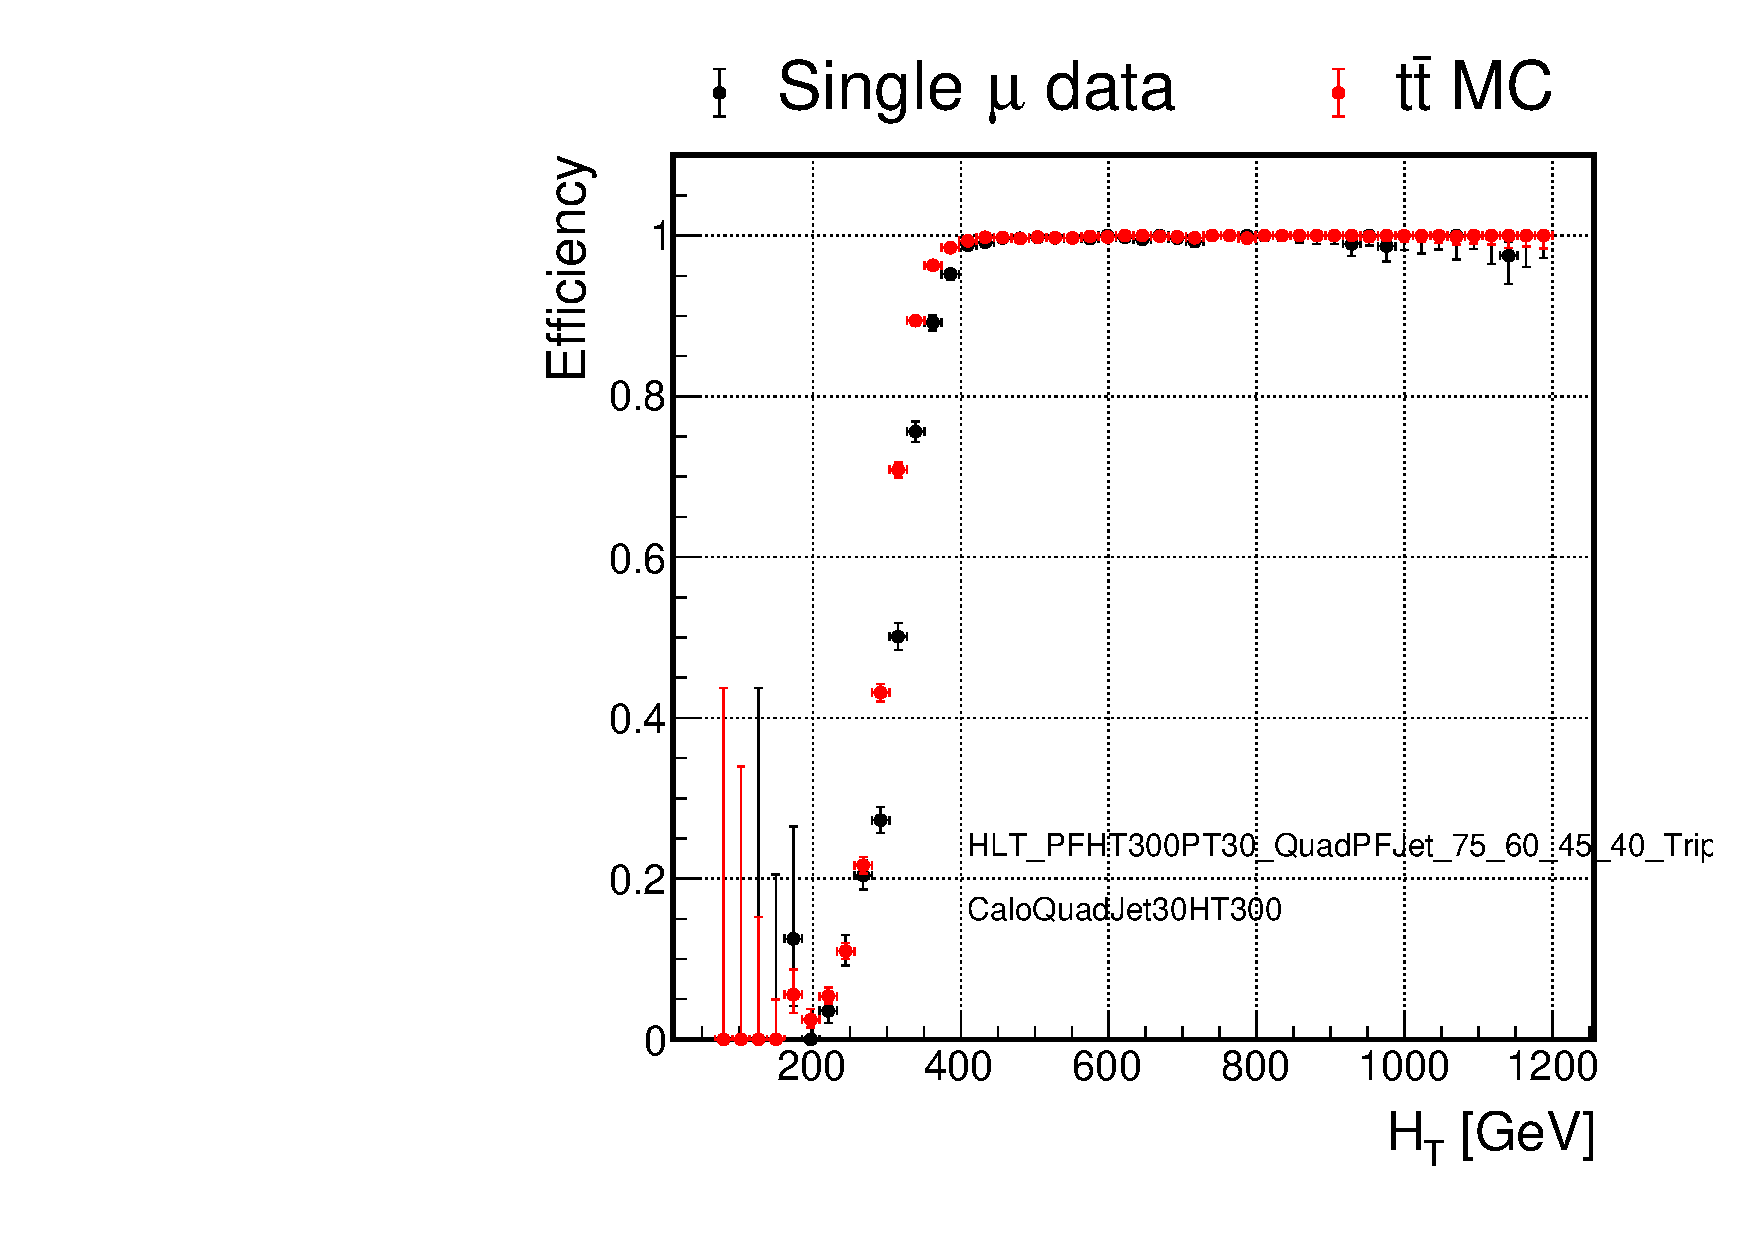
\includegraphics[width=0.3\textwidth]{Figures/AnalysisStrategy/triggereff/plots_2017/Quad_75_60_45_40_3b_Efficiency_CaloQuadJet30HT300.pdf}}\\
\subfloat{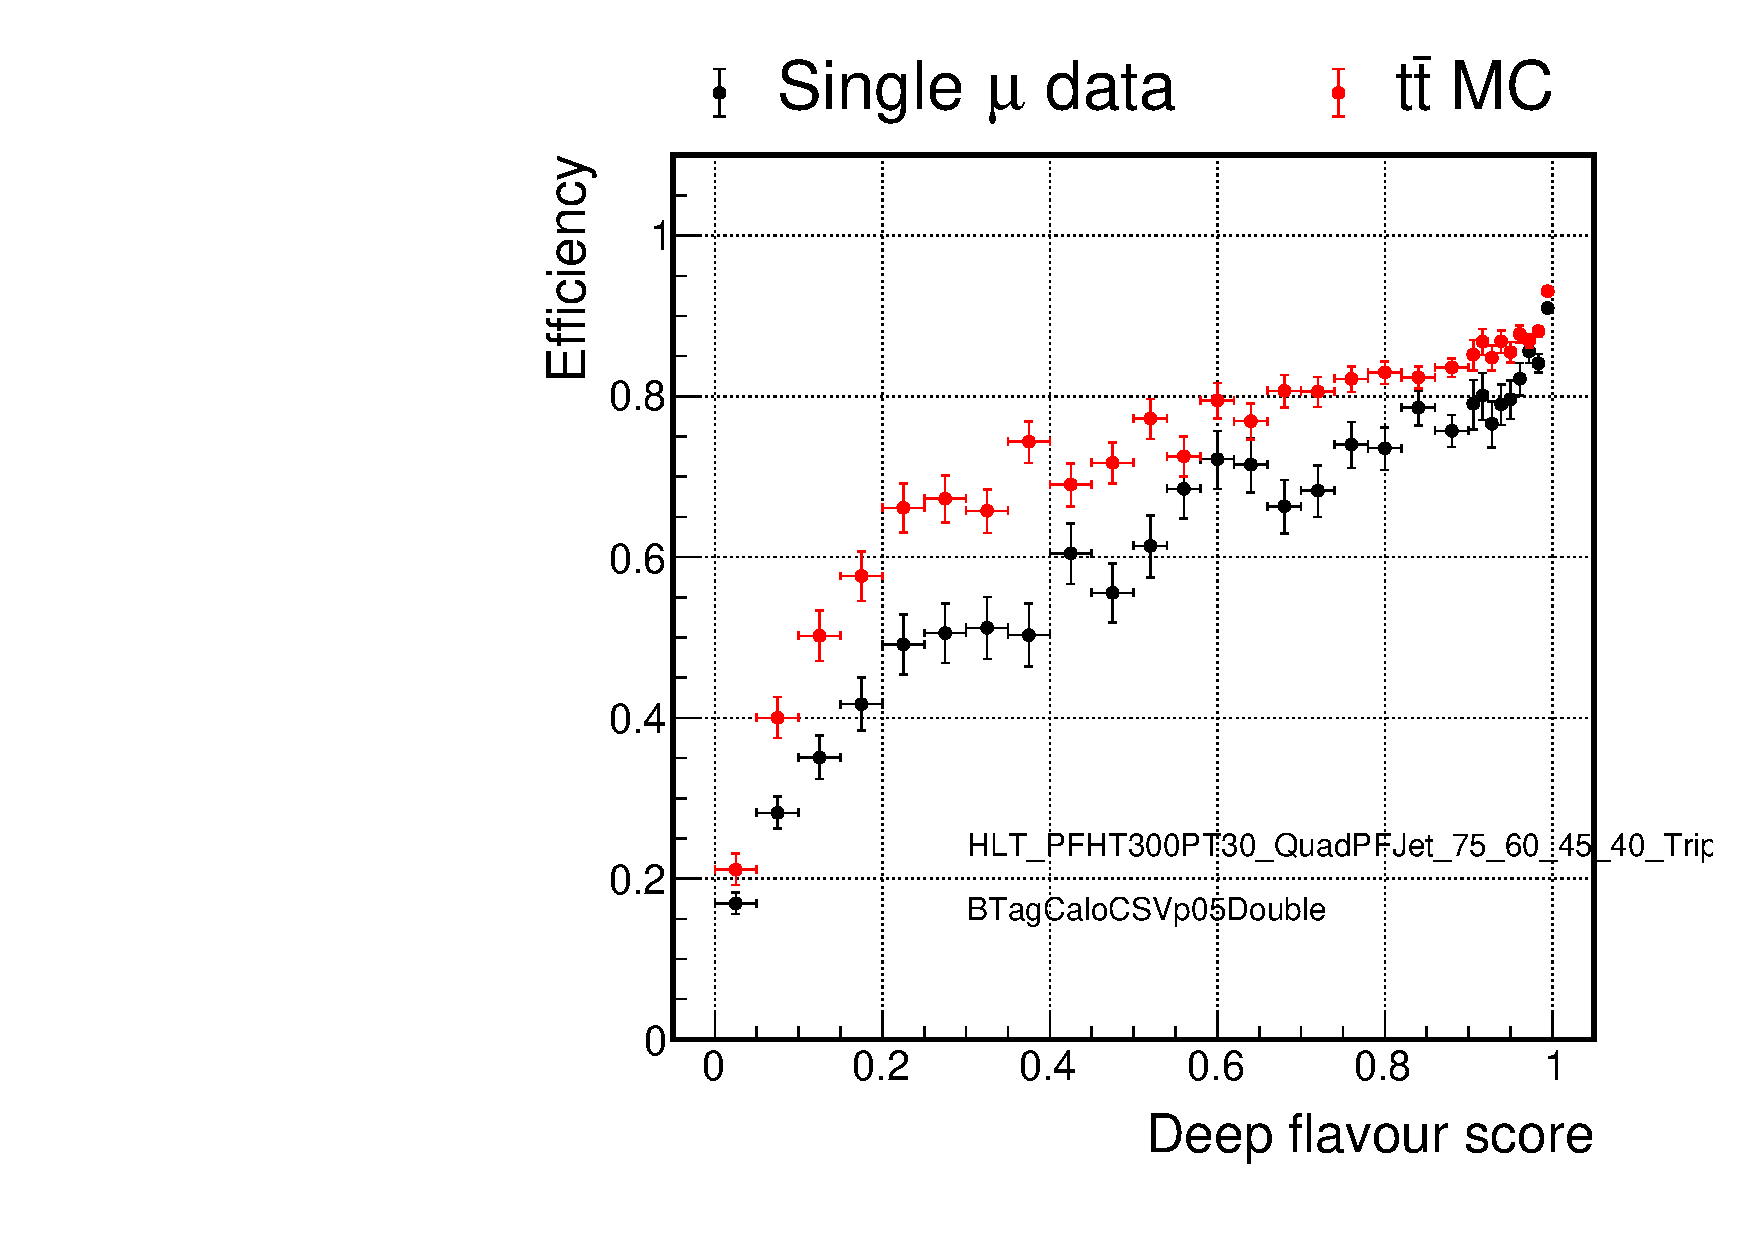
\includegraphics[width=0.3\textwidth]{Figures/AnalysisStrategy/triggereff/plots_2017/Quad_75_60_45_40_3b_Efficiency_BTagCaloCSVp05Double.pdf}}
\subfloat{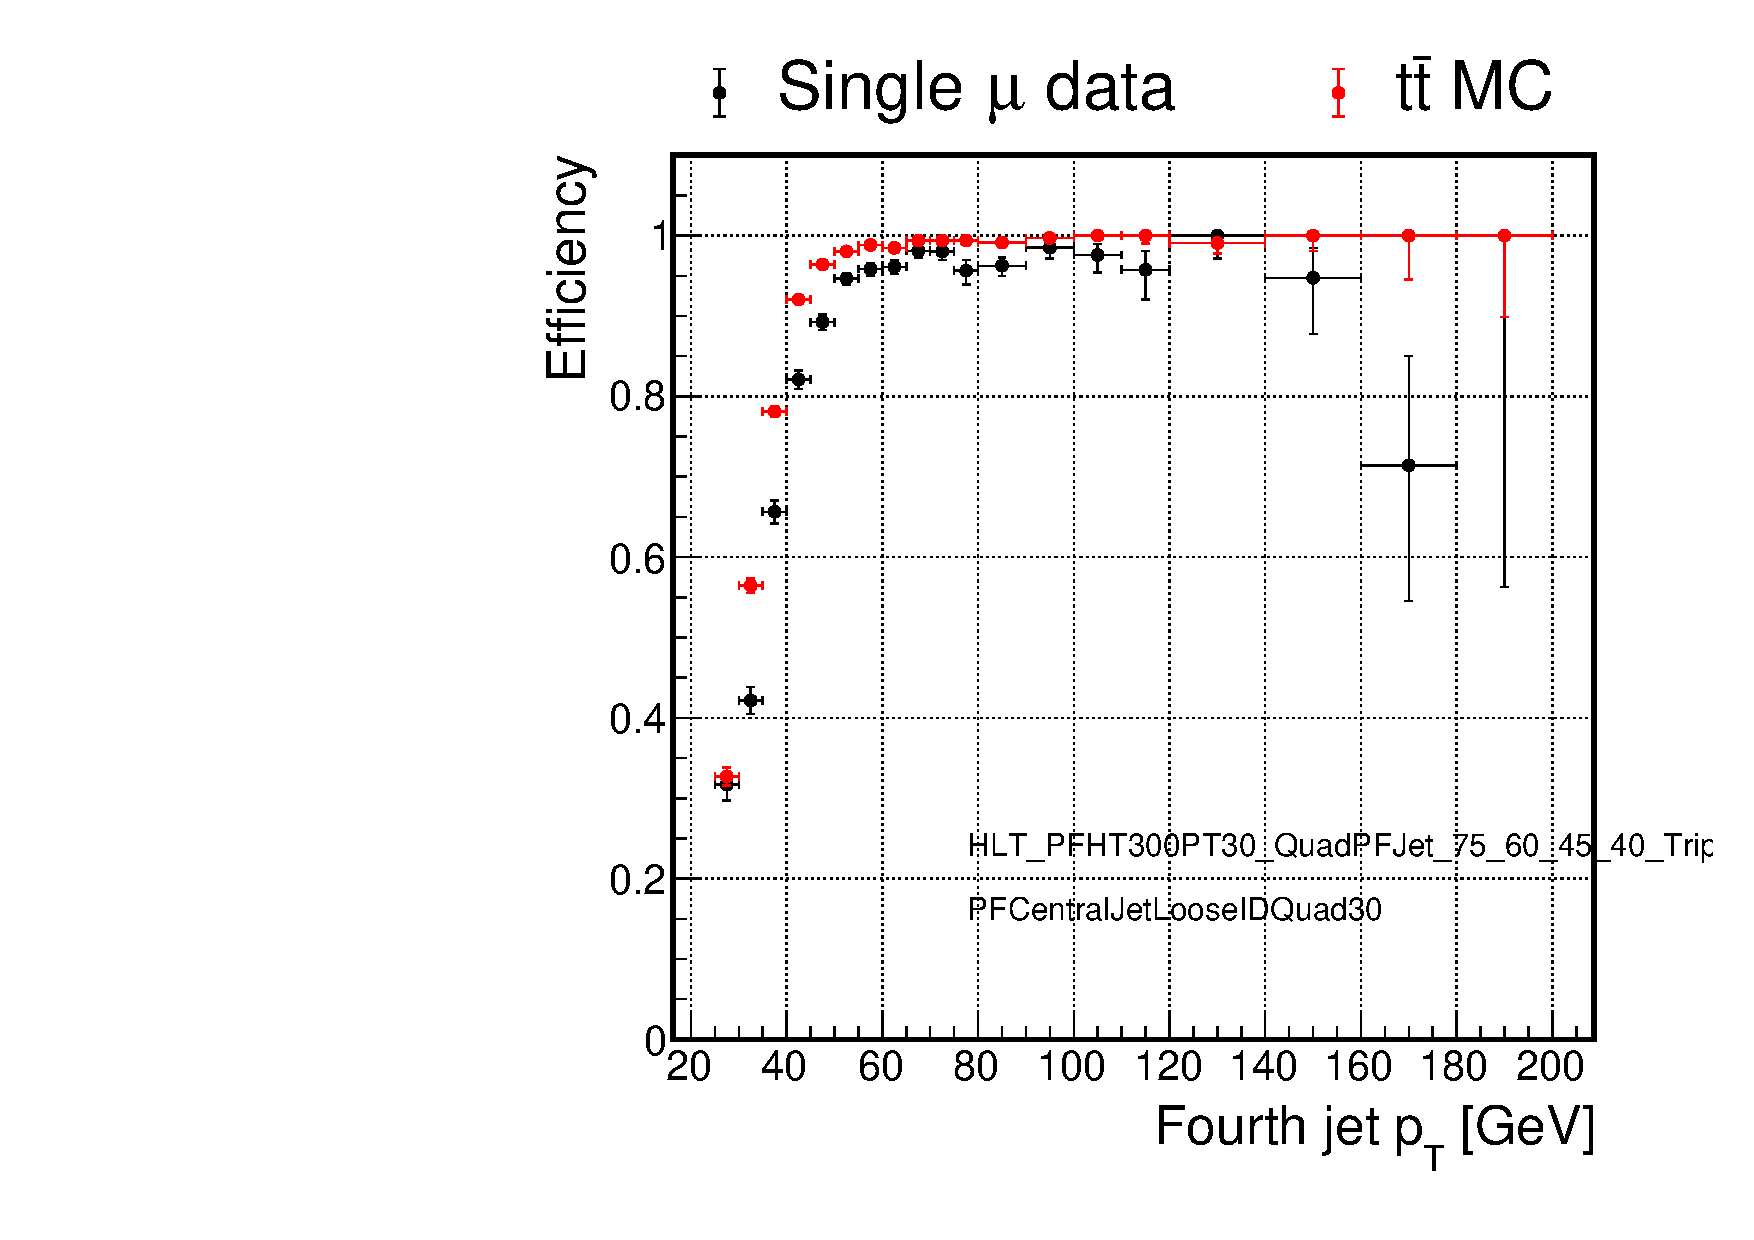
\includegraphics[width=0.3\textwidth]{Figures/AnalysisStrategy/triggereff/plots_2017/Quad_75_60_45_40_3b_Efficiency_PFCentralJetLooseIDQuad30.pdf}}
\subfloat{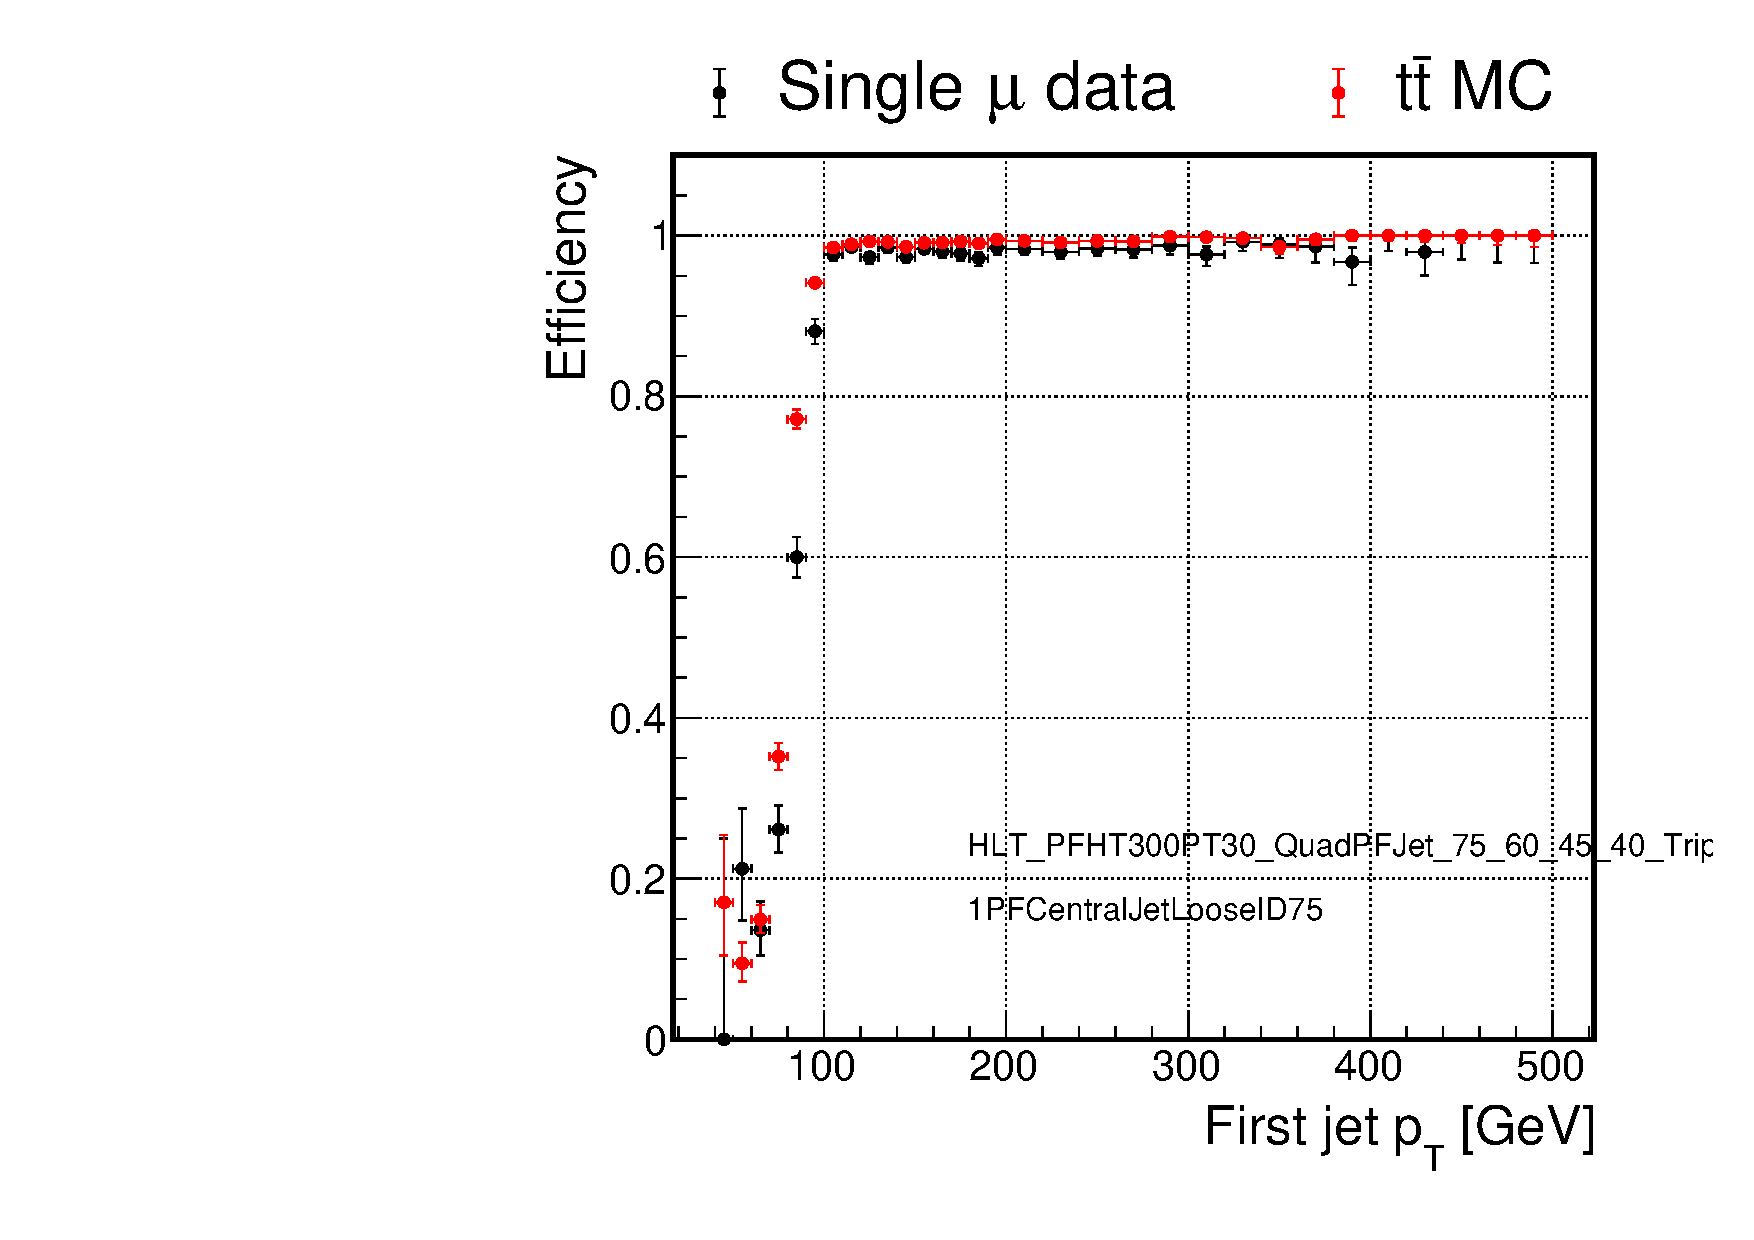
\includegraphics[width=0.3\textwidth]{Figures/AnalysisStrategy/triggereff/plots_2017/Quad_75_60_45_40_3b_Efficiency_1PFCentralJetLooseID75.pdf}}\\
\subfloat{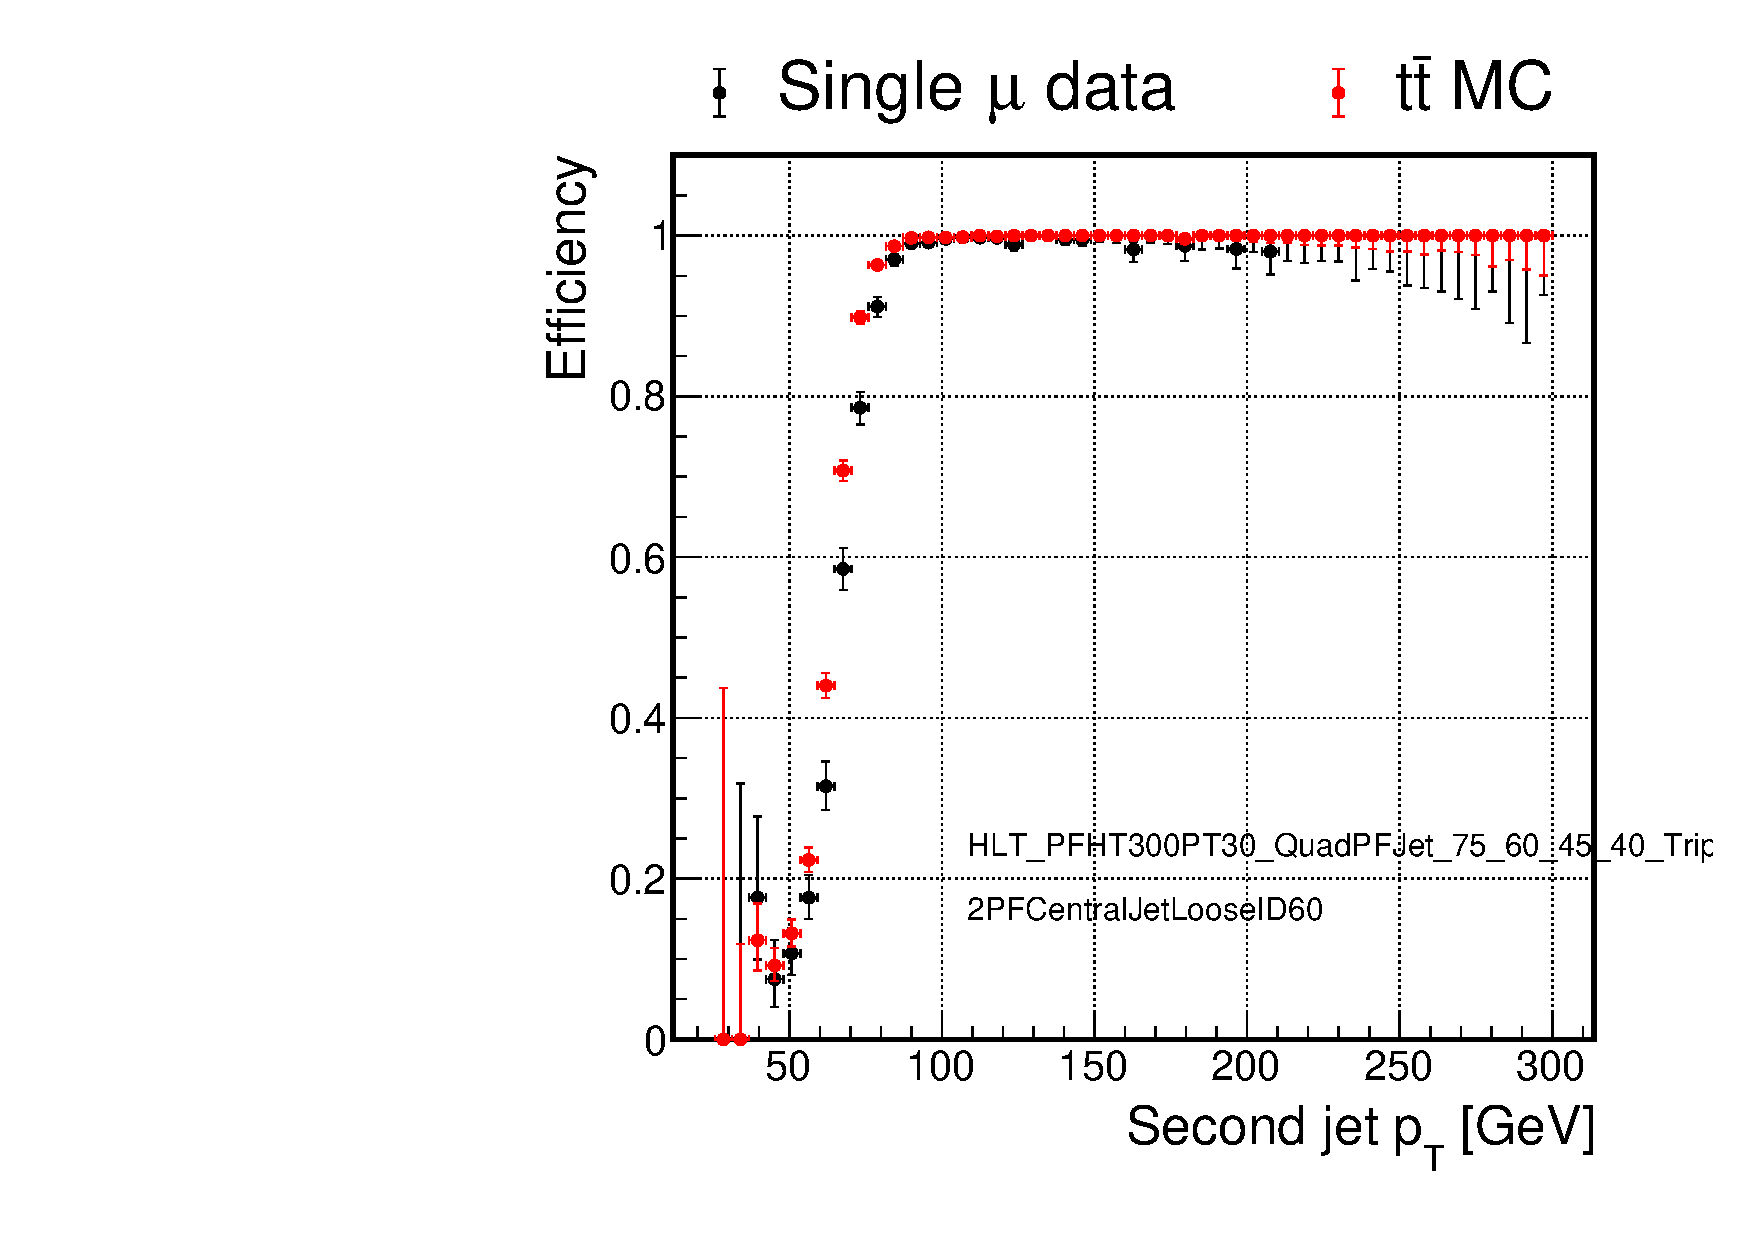
\includegraphics[width=0.3\textwidth]{Figures/AnalysisStrategy/triggereff/plots_2017/Quad_75_60_45_40_3b_Efficiency_2PFCentralJetLooseID60.pdf}}
\subfloat{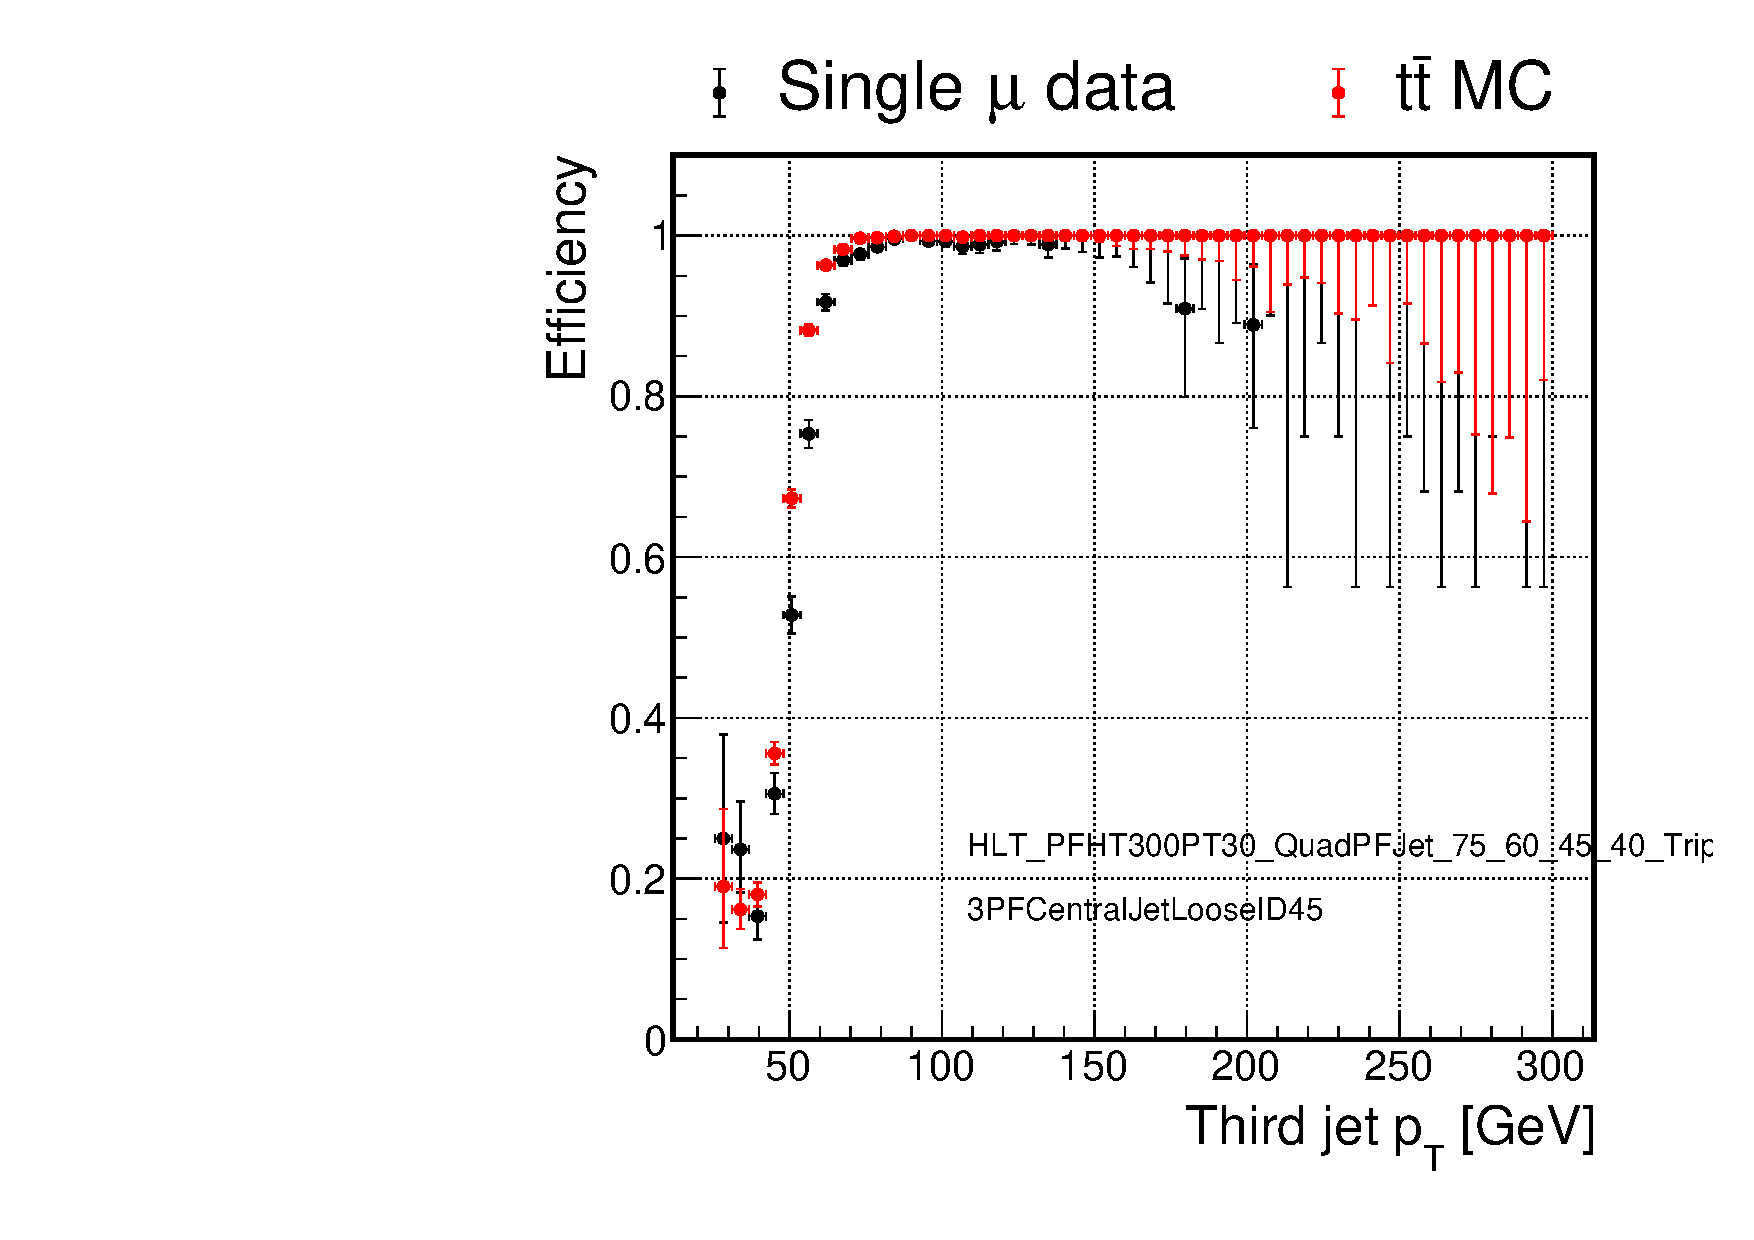
\includegraphics[width=0.3\textwidth]{Figures/AnalysisStrategy/triggereff/plots_2017/Quad_75_60_45_40_3b_Efficiency_3PFCentralJetLooseID45.pdf}}
\subfloat{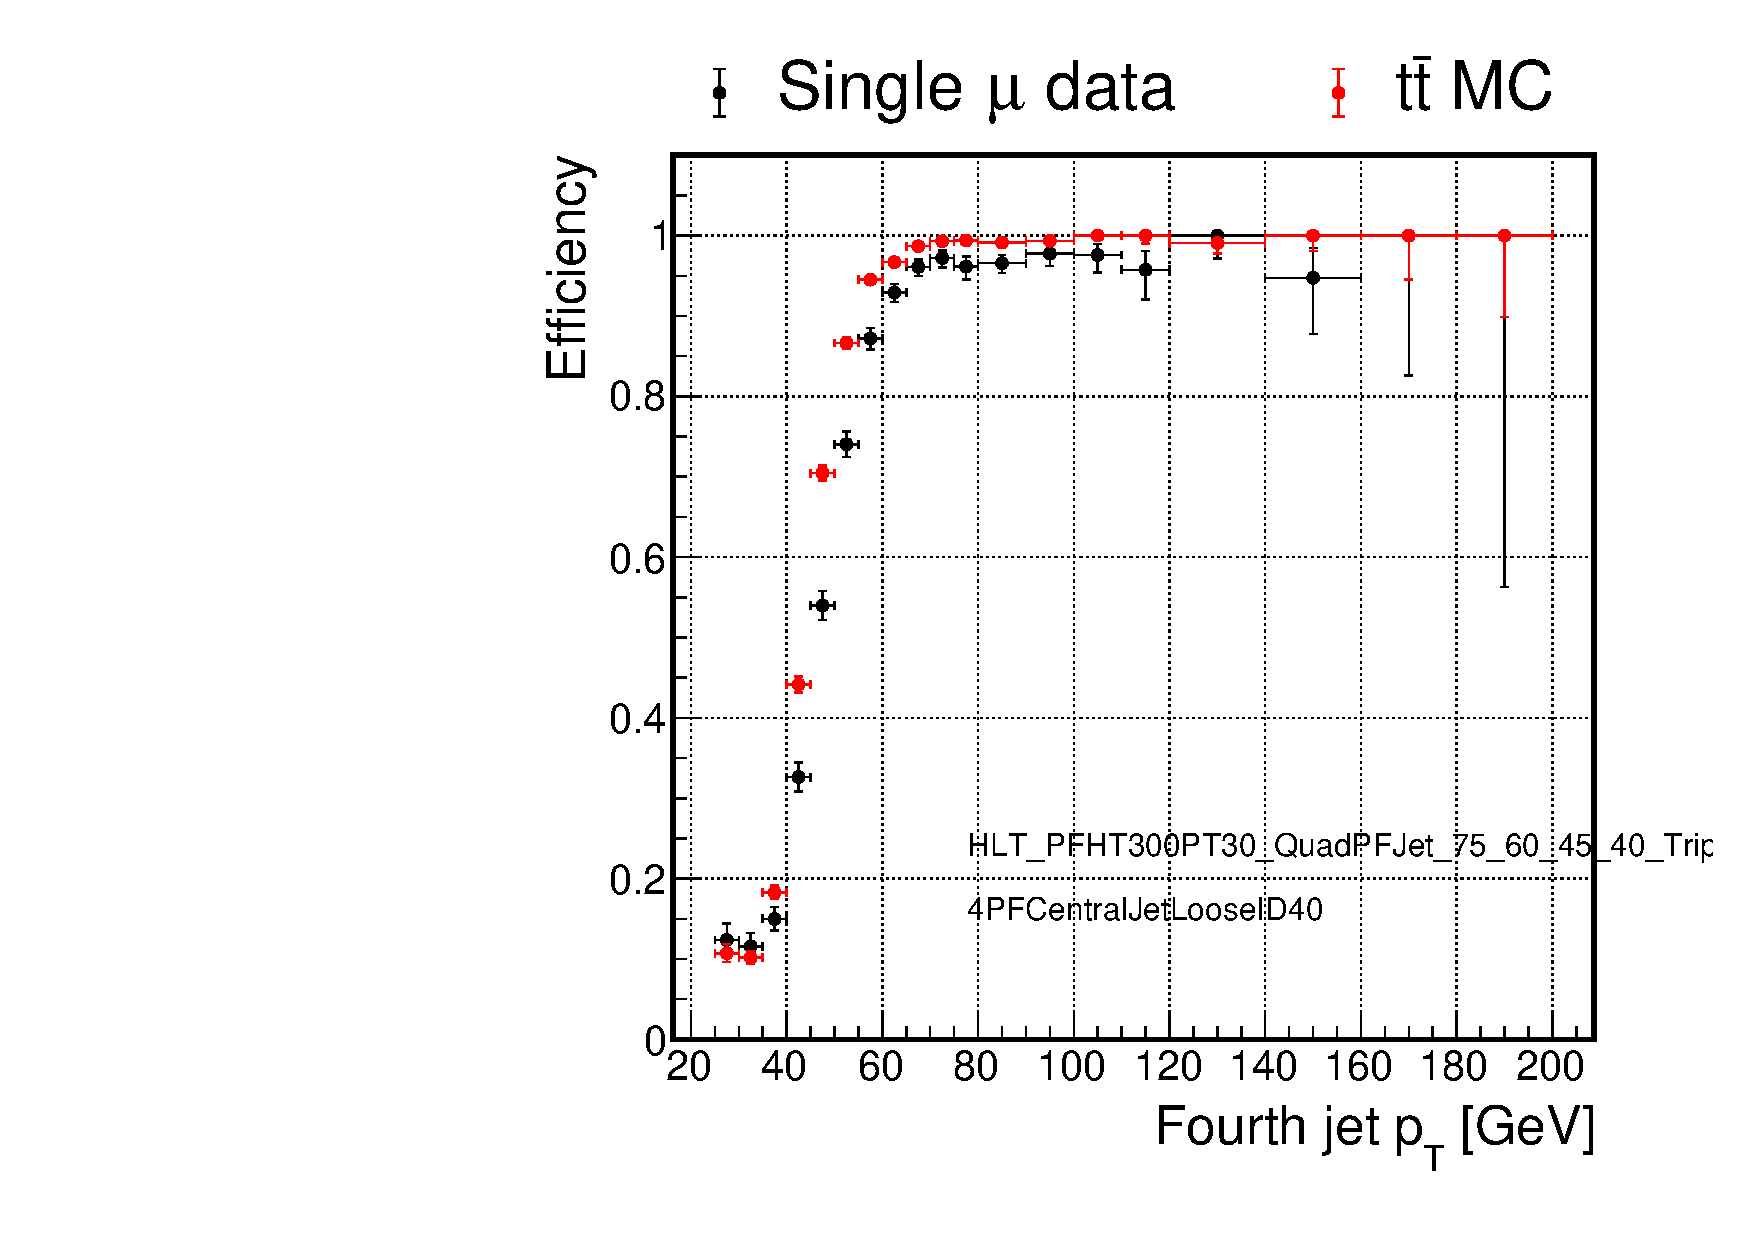
\includegraphics[width=0.3\textwidth]{Figures/AnalysisStrategy/triggereff/plots_2017/Quad_75_60_45_40_3b_Efficiency_4PFCentralJetLooseID40.pdf}}\\
\subfloat{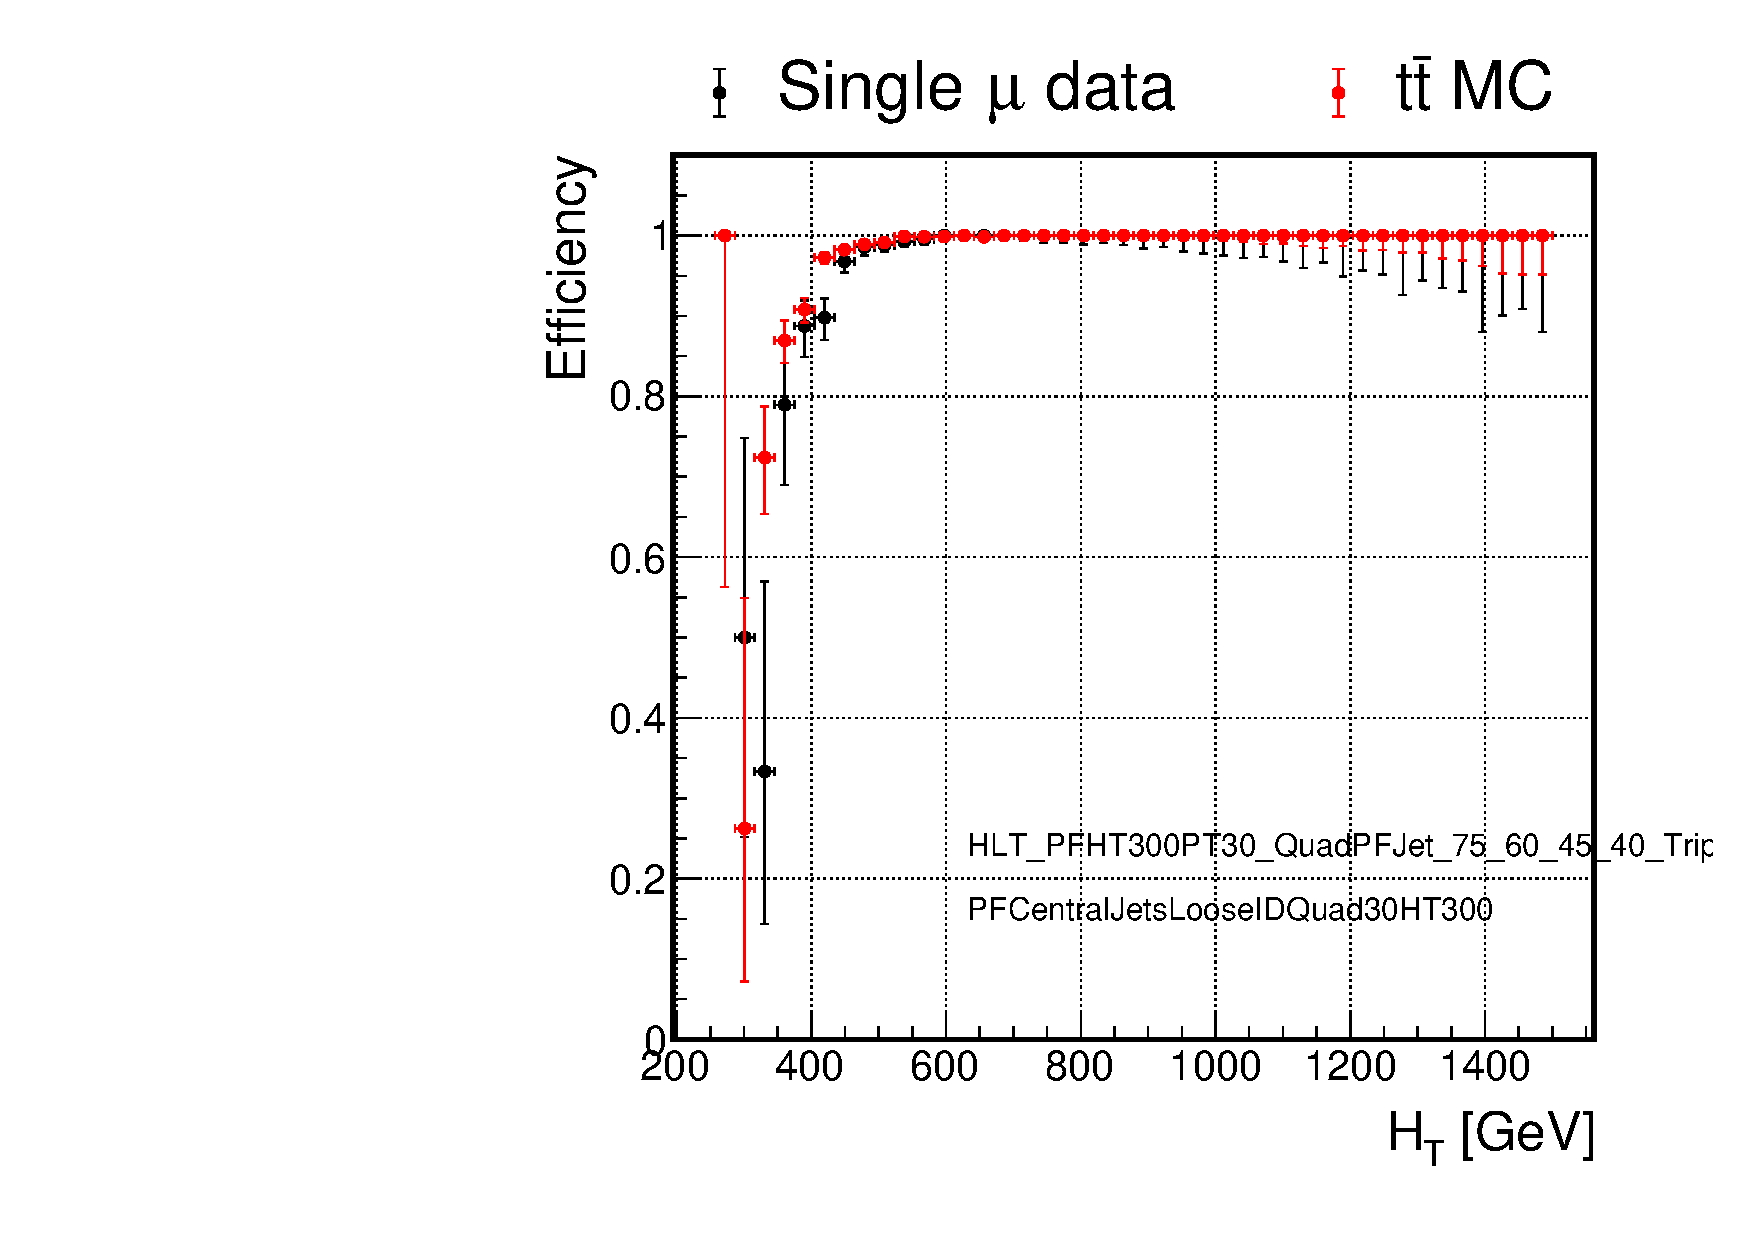
\includegraphics[width=0.3\textwidth]{Figures/AnalysisStrategy/triggereff/plots_2017/Quad_75_60_45_40_3b_Efficiency_PFCentralJetsLooseIDQuad30HT300.pdf}}
\subfloat{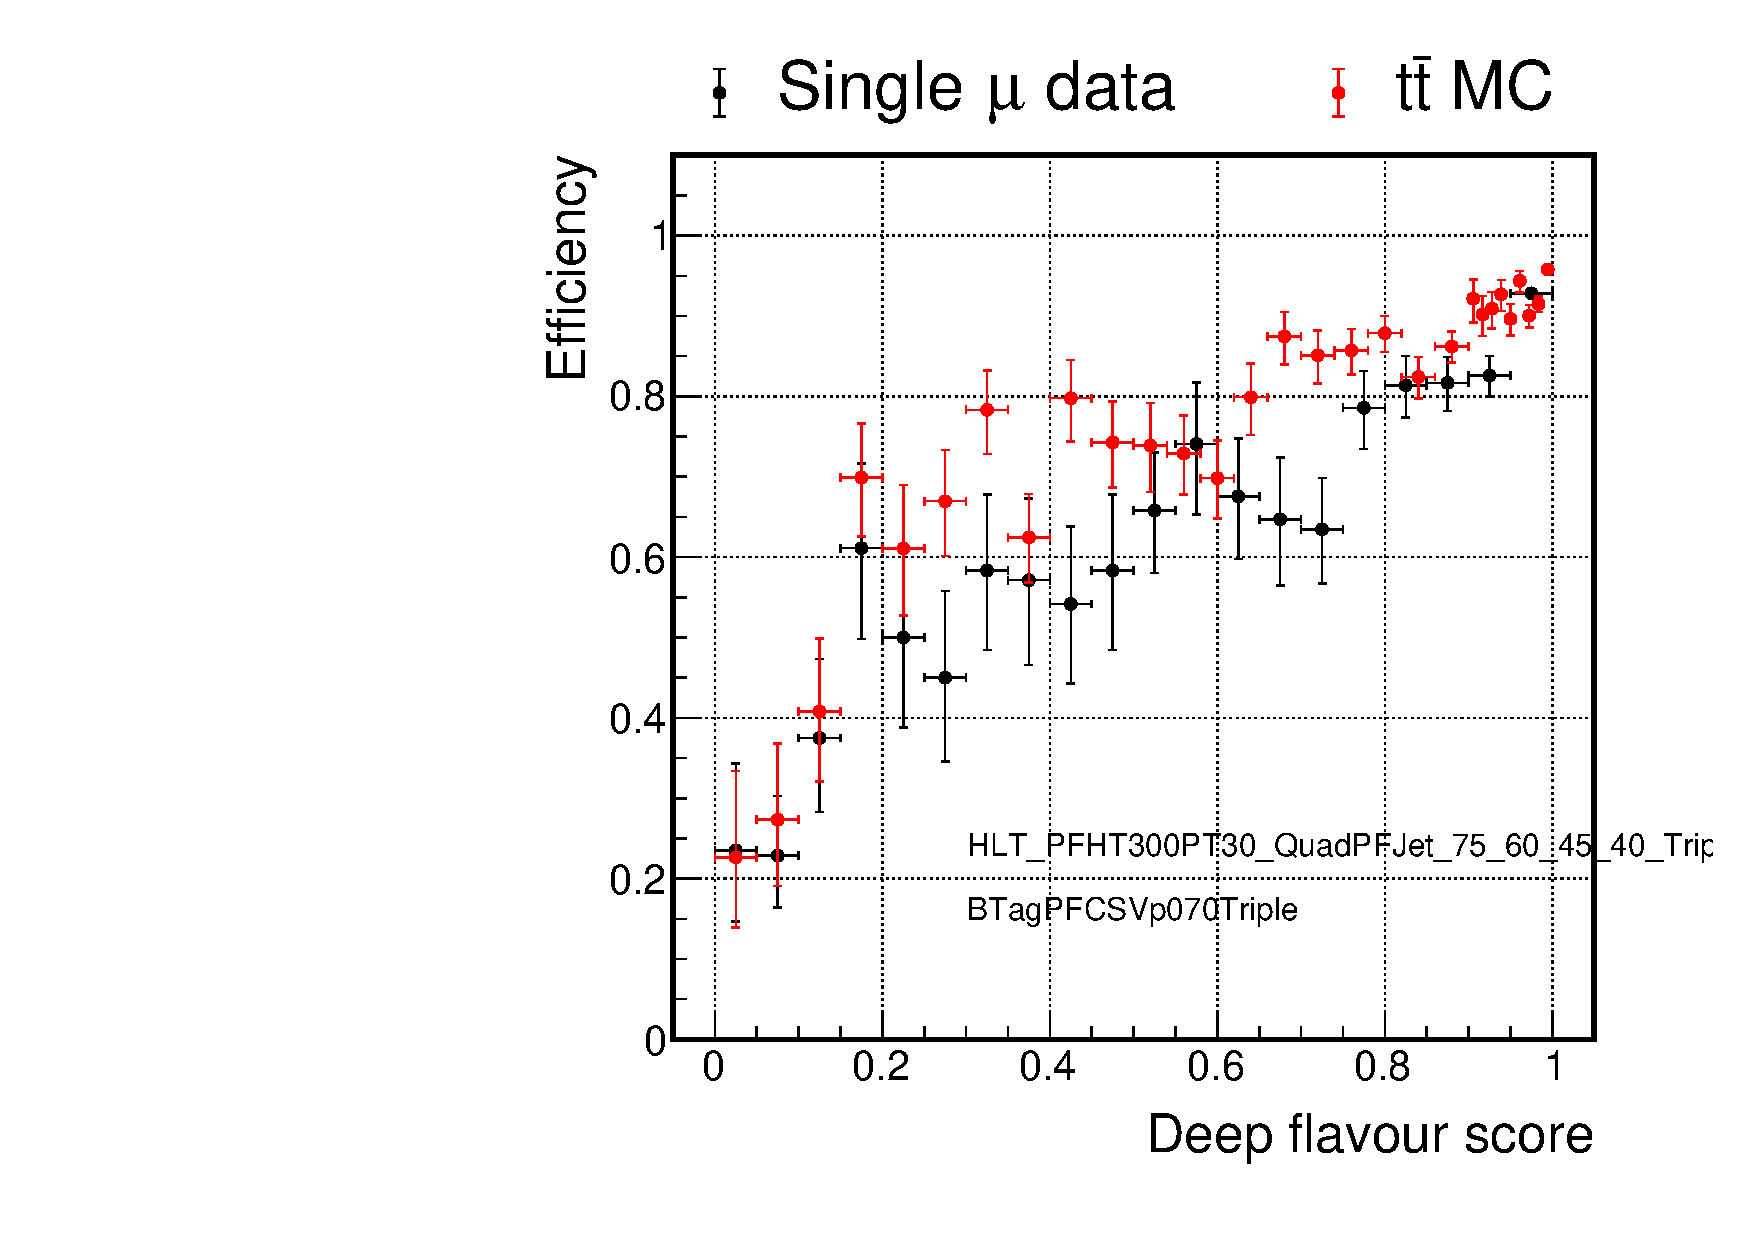
\includegraphics[width=0.3\textwidth]{Figures/AnalysisStrategy/triggereff/plots_2017/Quad_75_60_45_40_3b_Efficiency_BTagPFCSVp070Triple.pdf}}
\caption[Efficiency measured in single muon data and $\ttbar$ MC for filters of the HLT\_PFHT300PT30\_QuadPFJet\_75\_60\_45\_40\_TriplePFBTagCSV path in 2017]{Efficiency measured in single muon data (black) and $\ttbar$ MC (red) for filters of HLT\_PFHT300PT30\_QuadPFJet\_75\_60\_45\_40\_TriplePFBTagCSV, corresponding to the 2017 dataset.}
\label{trigger:fig:filterEfficiency2017}
\end{figure}

\begin{figure}[p]
\centering
\subfloat{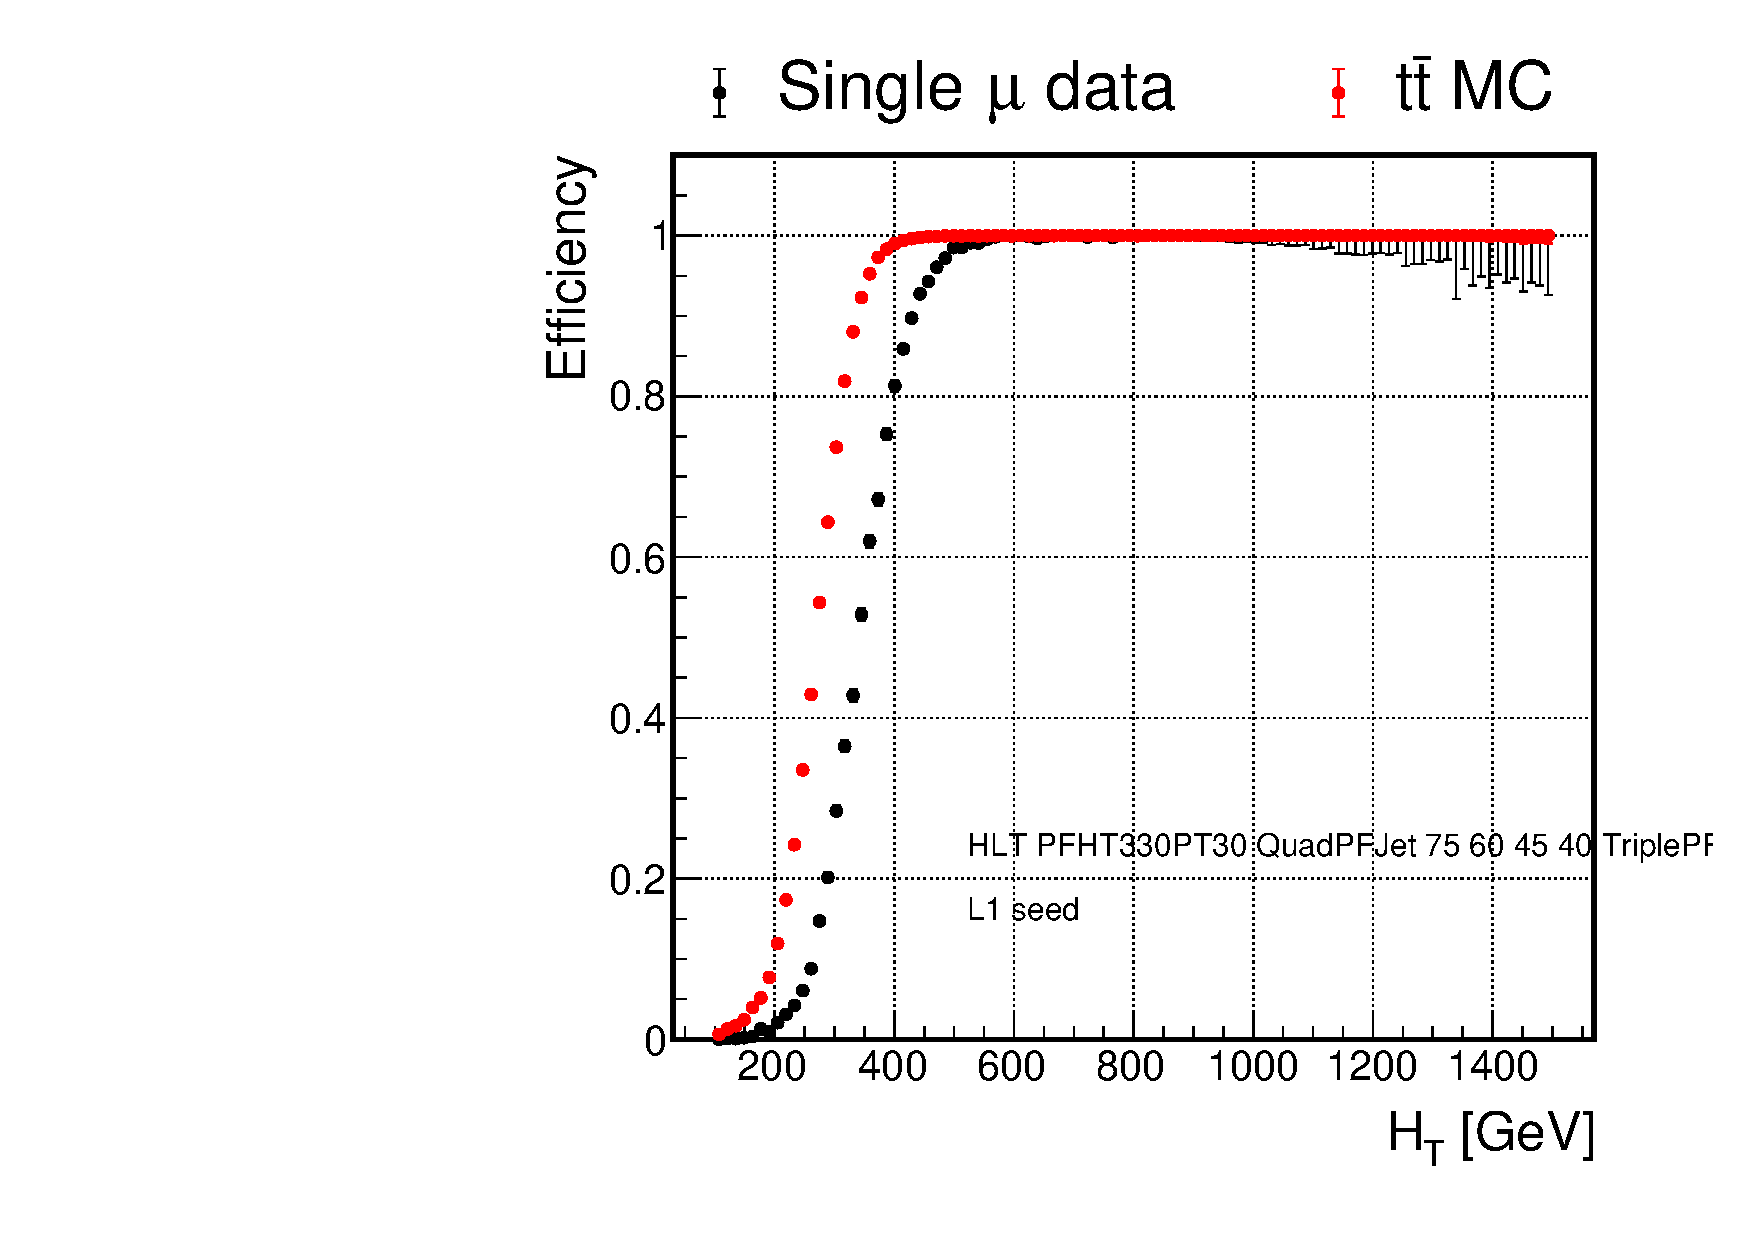
\includegraphics[width=0.3\textwidth]{Figures/AnalysisStrategy/triggereff/plots_2018/Quad_75_60_45_40_3b_Efficiency_L1filterHT.pdf}}
\subfloat{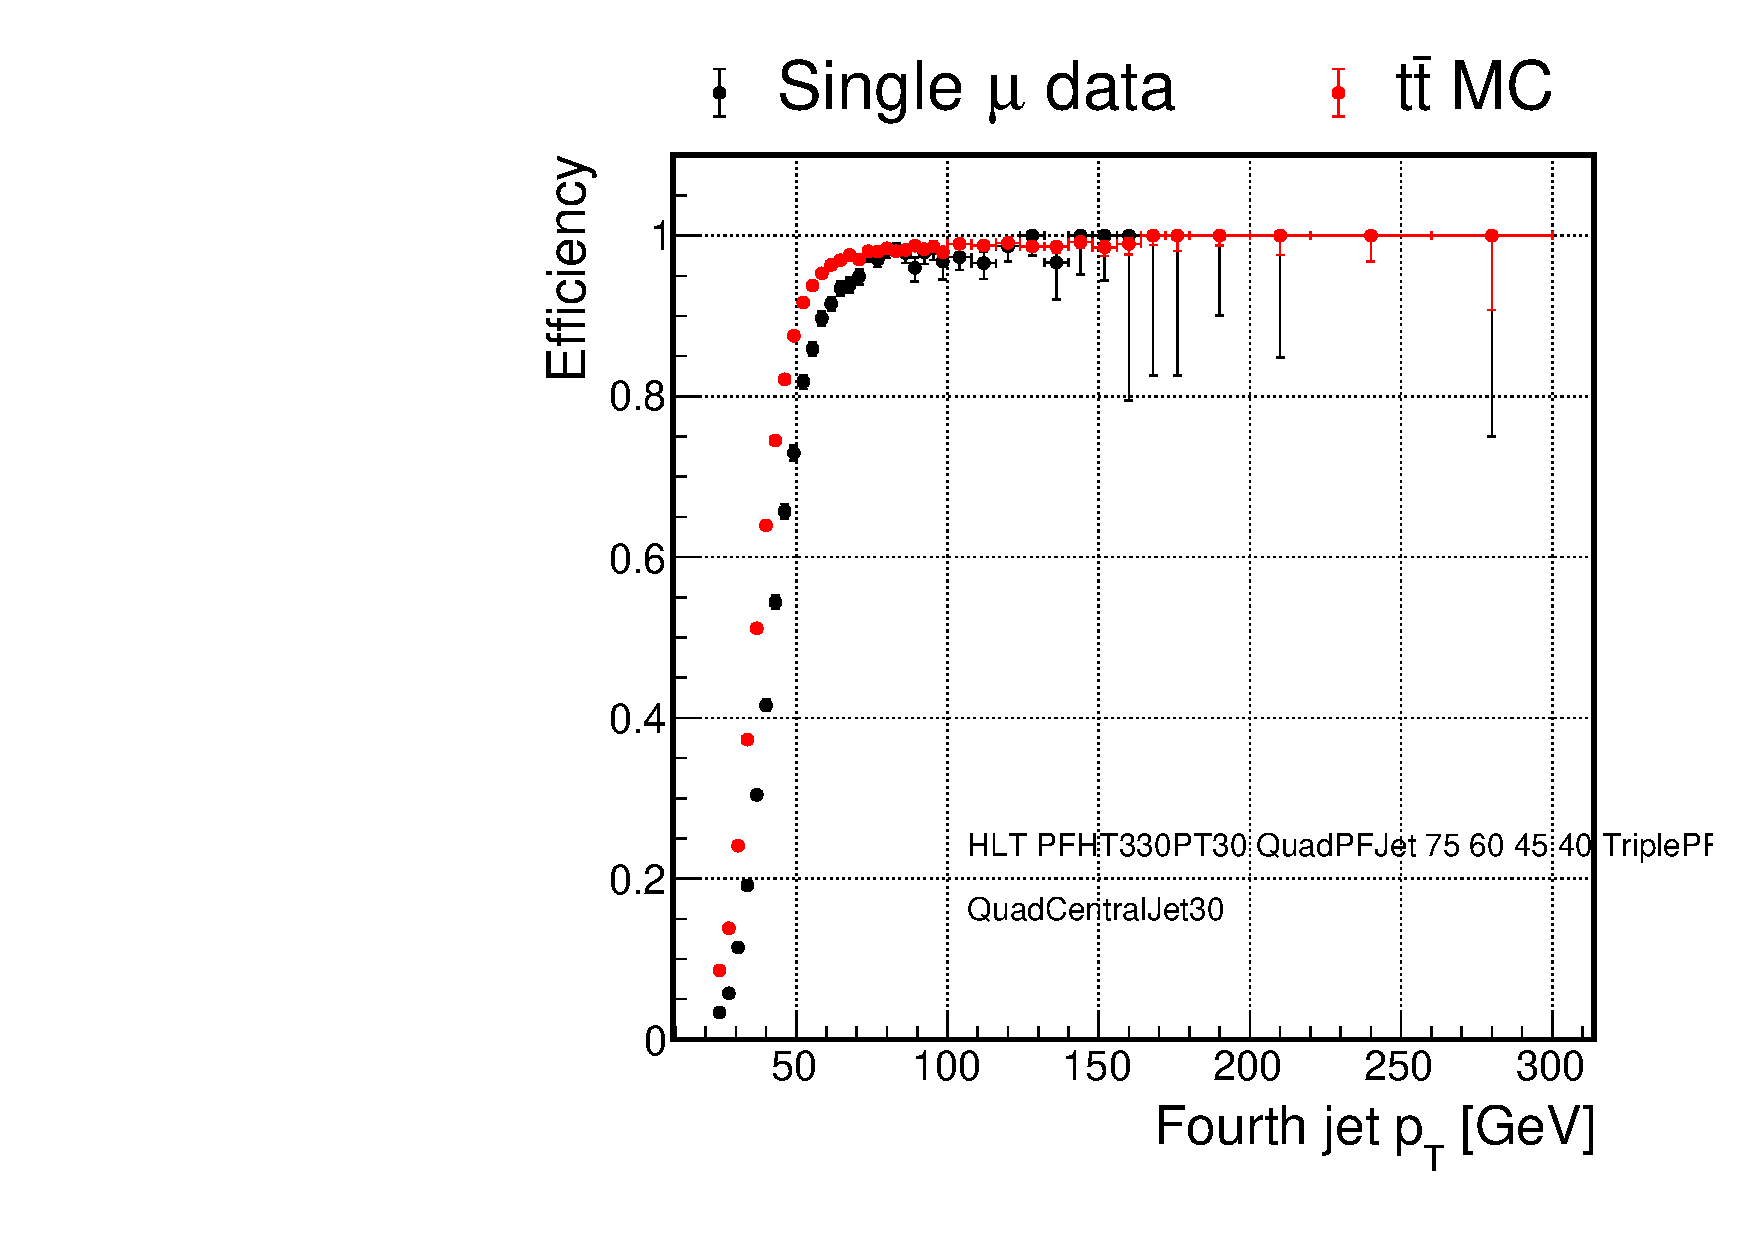
\includegraphics[width=0.3\textwidth]{Figures/AnalysisStrategy/triggereff/plots_2018/Quad_75_60_45_40_3b_Efficiency_QuadCentralJet30.pdf}}
\subfloat{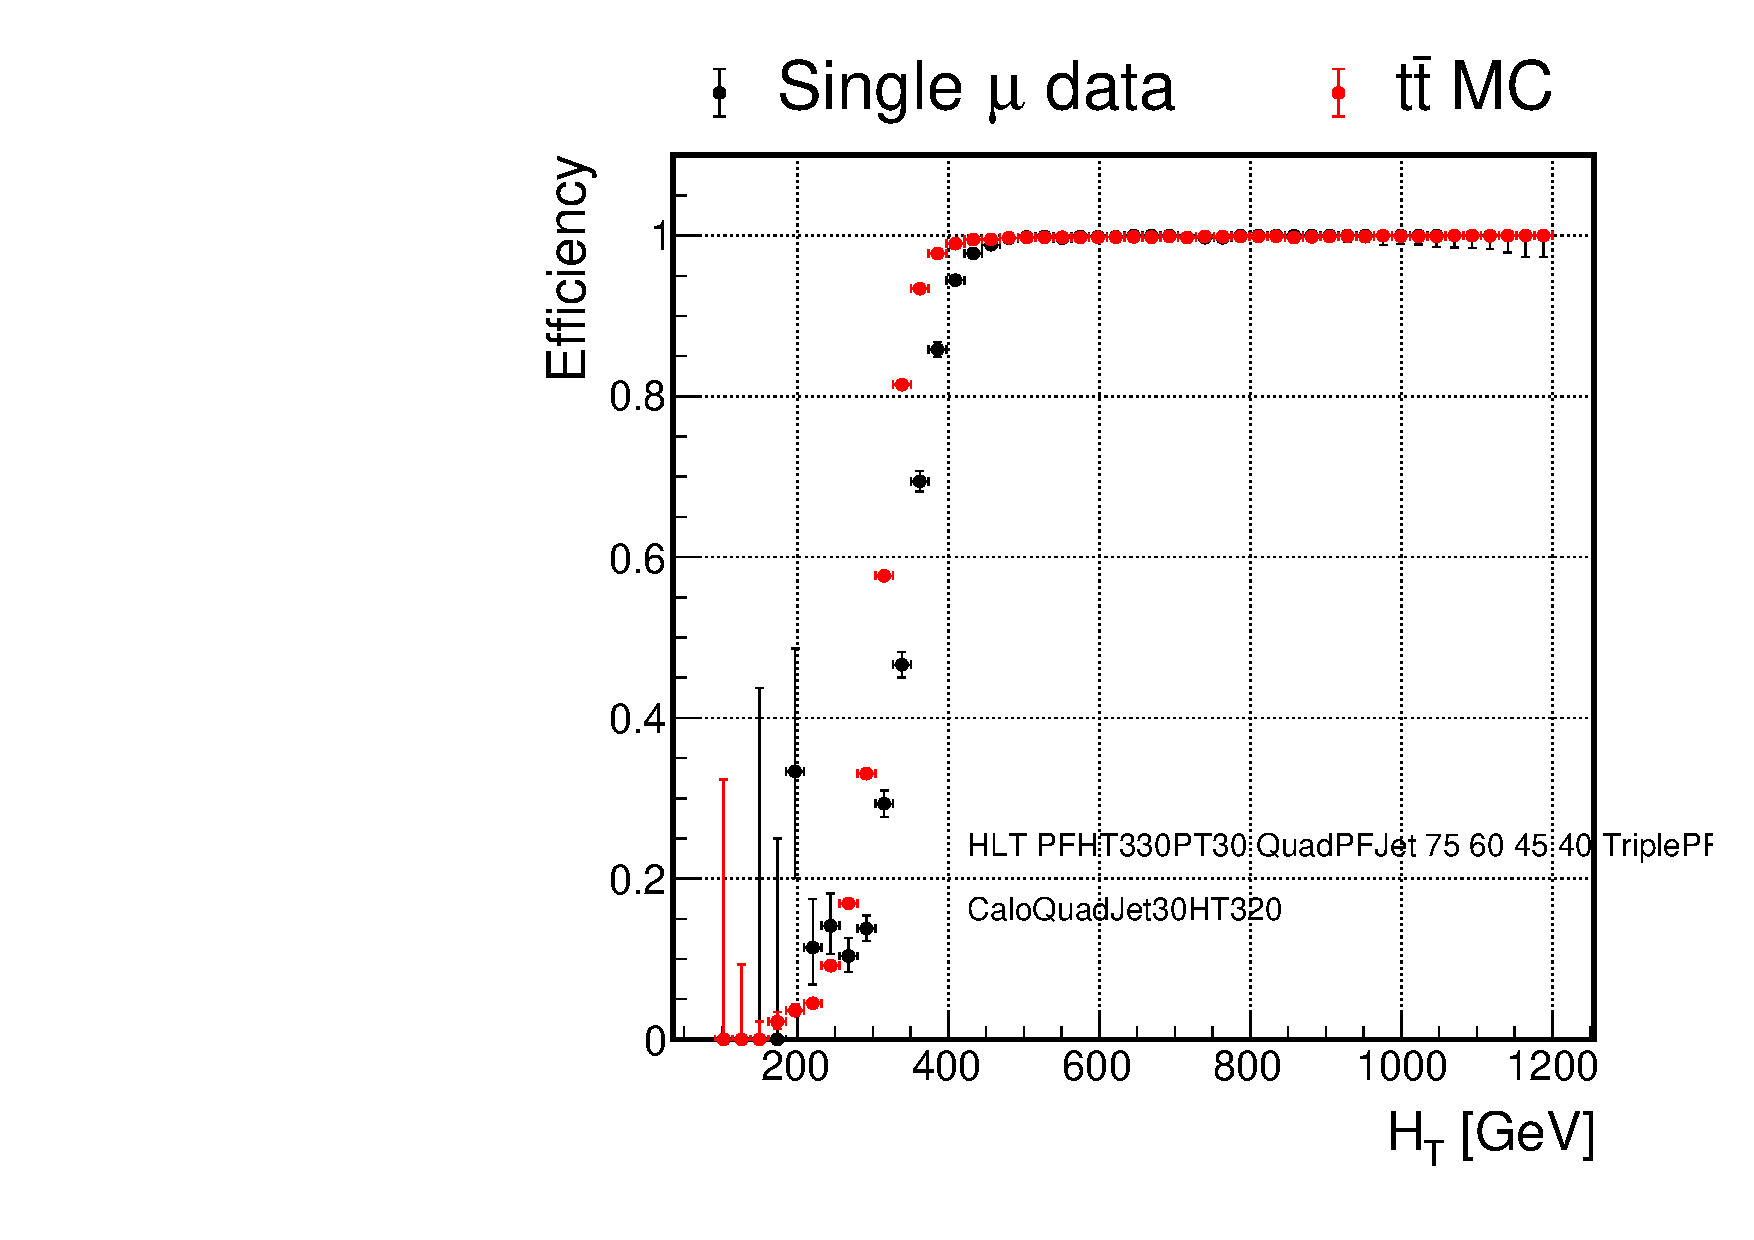
\includegraphics[width=0.3\textwidth]{Figures/AnalysisStrategy/triggereff/plots_2018/Quad_75_60_45_40_3b_Efficiency_CaloQuadJet30HT320.pdf}}\\
\subfloat{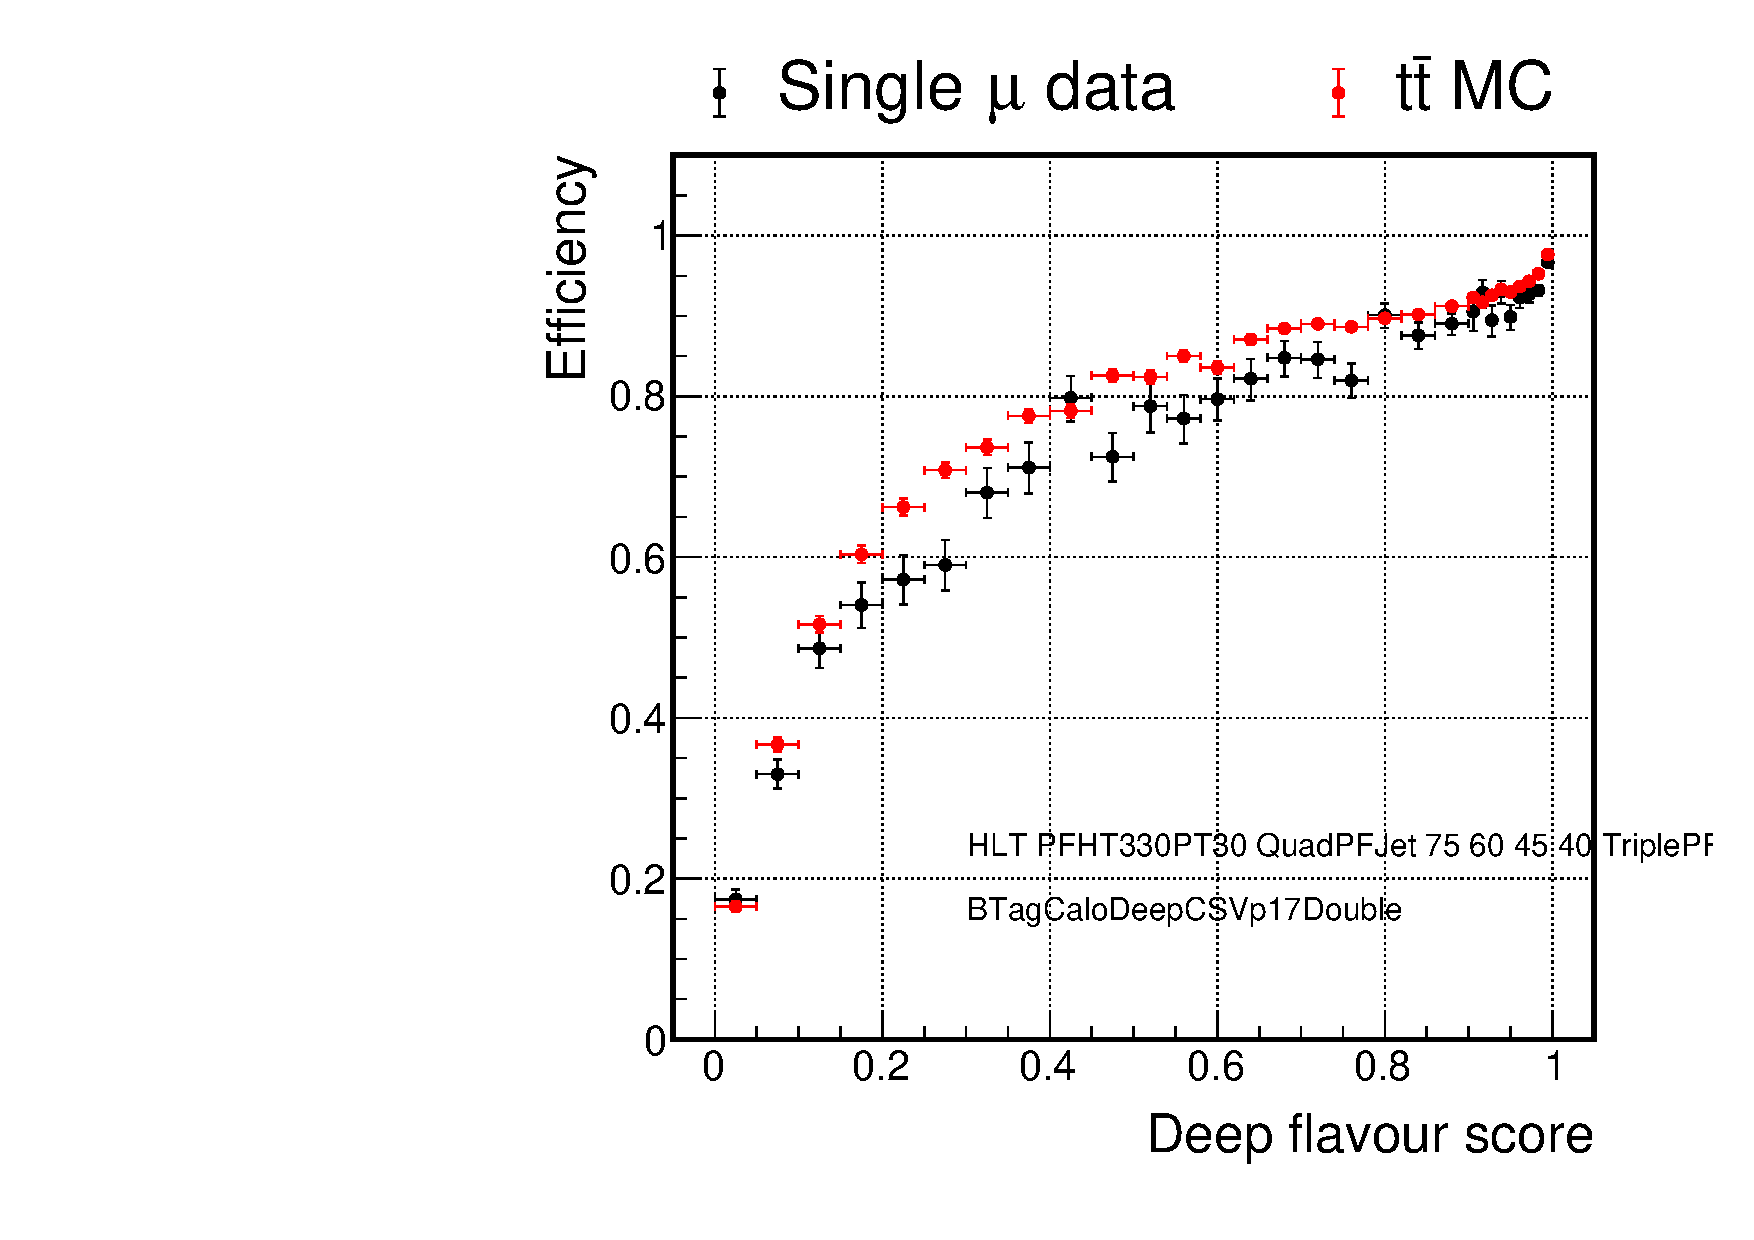
\includegraphics[width=0.3\textwidth]{Figures/AnalysisStrategy/triggereff/plots_2018/Quad_75_60_45_40_3b_Efficiency_BTagCaloDeepCSVp17Double.pdf}}
\subfloat{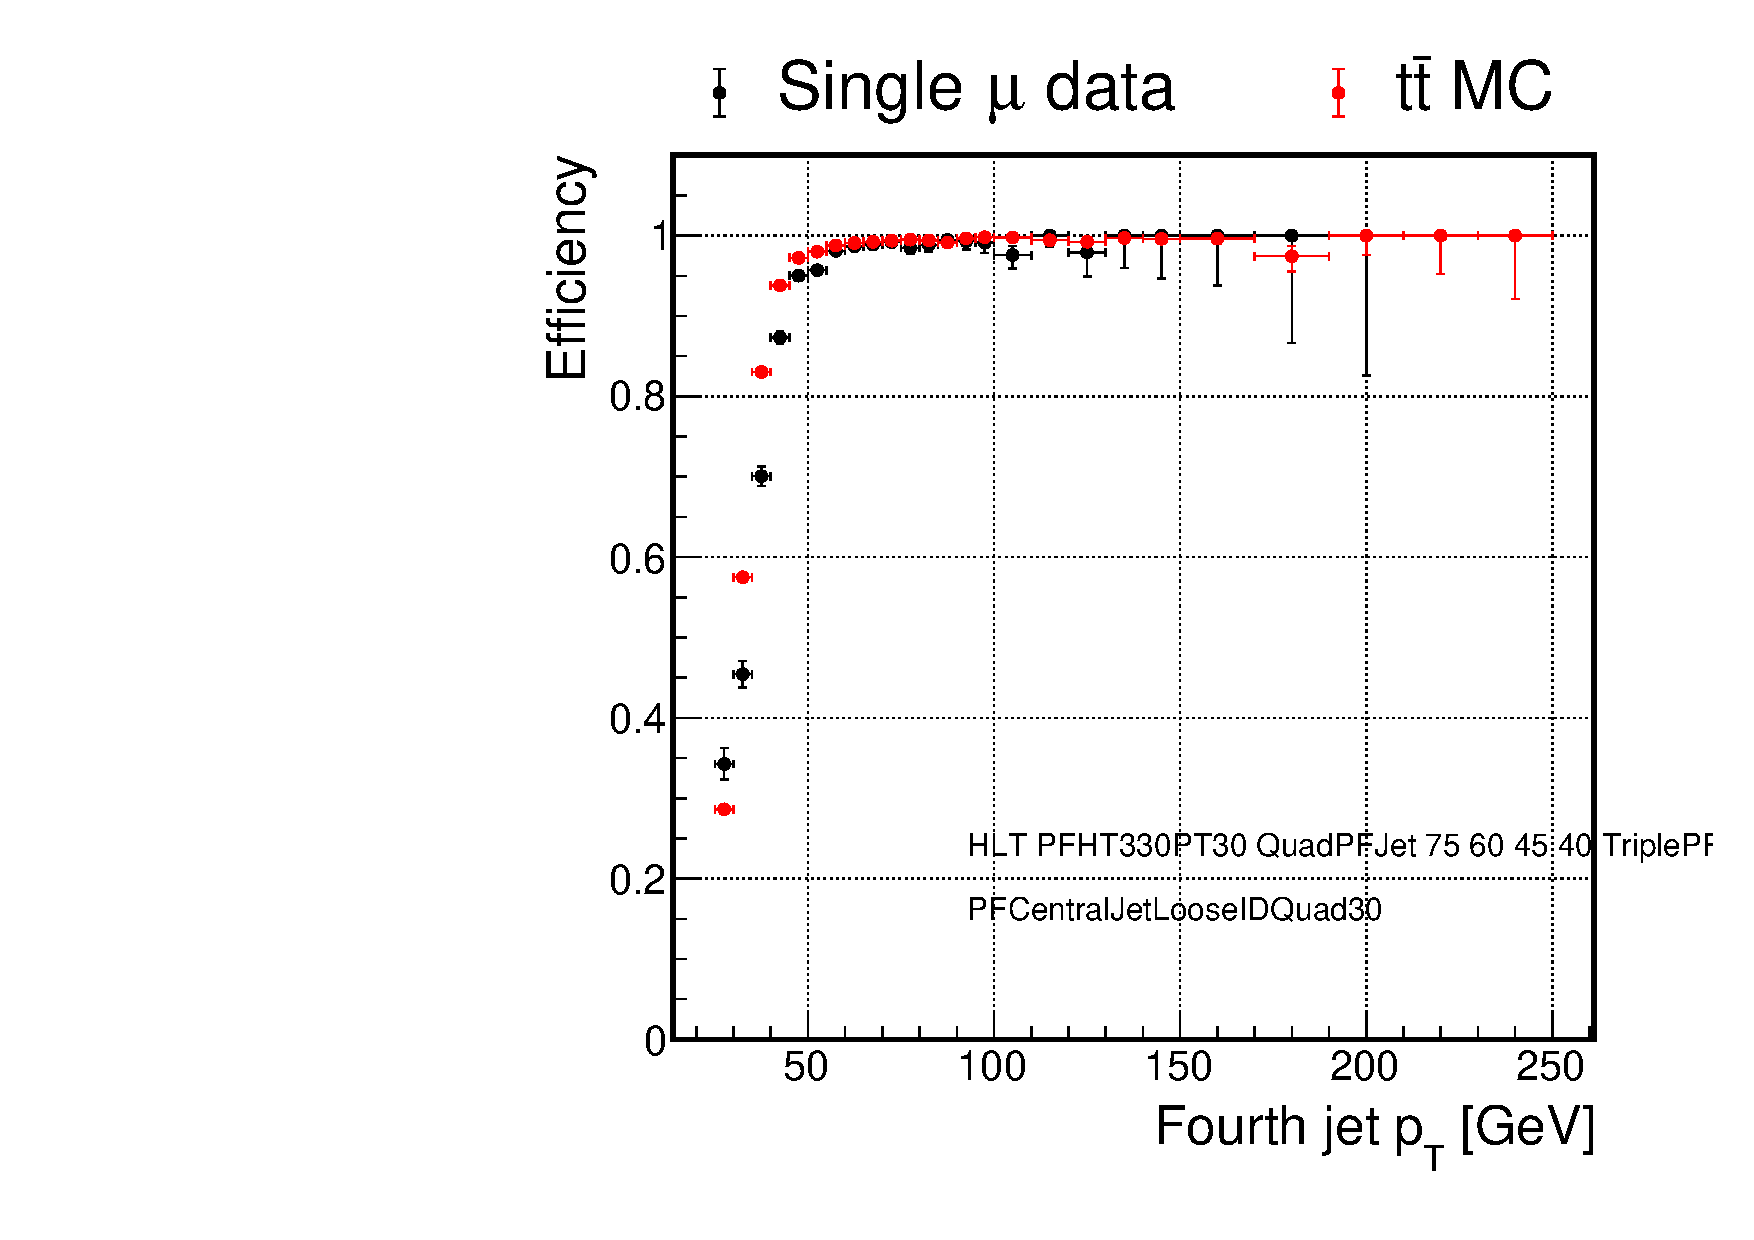
\includegraphics[width=0.3\textwidth]{Figures/AnalysisStrategy/triggereff/plots_2018/Quad_75_60_45_40_3b_Efficiency_PFCentralJetLooseIDQuad30.pdf}}
\subfloat{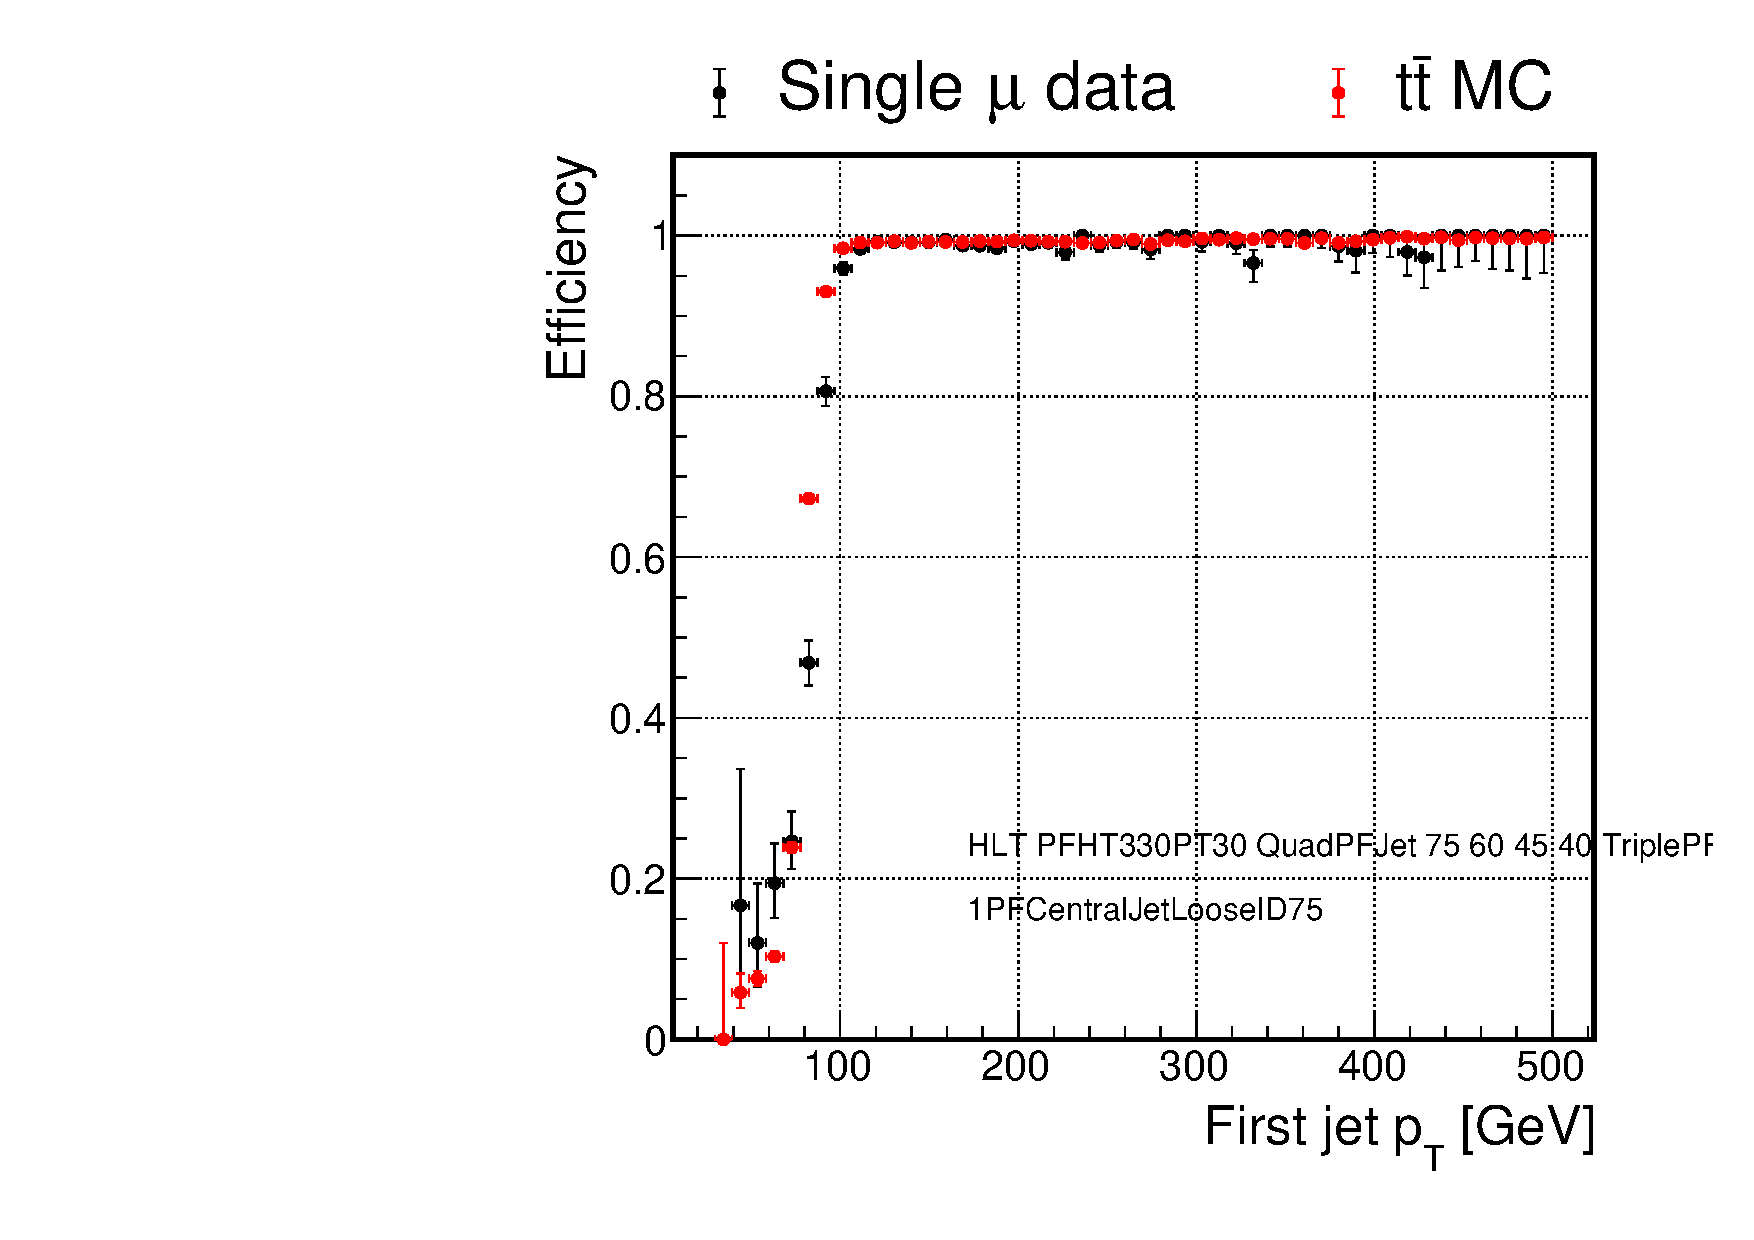
\includegraphics[width=0.3\textwidth]{Figures/AnalysisStrategy/triggereff/plots_2018/Quad_75_60_45_40_3b_Efficiency_1PFCentralJetLooseID75.pdf}}\\
\subfloat{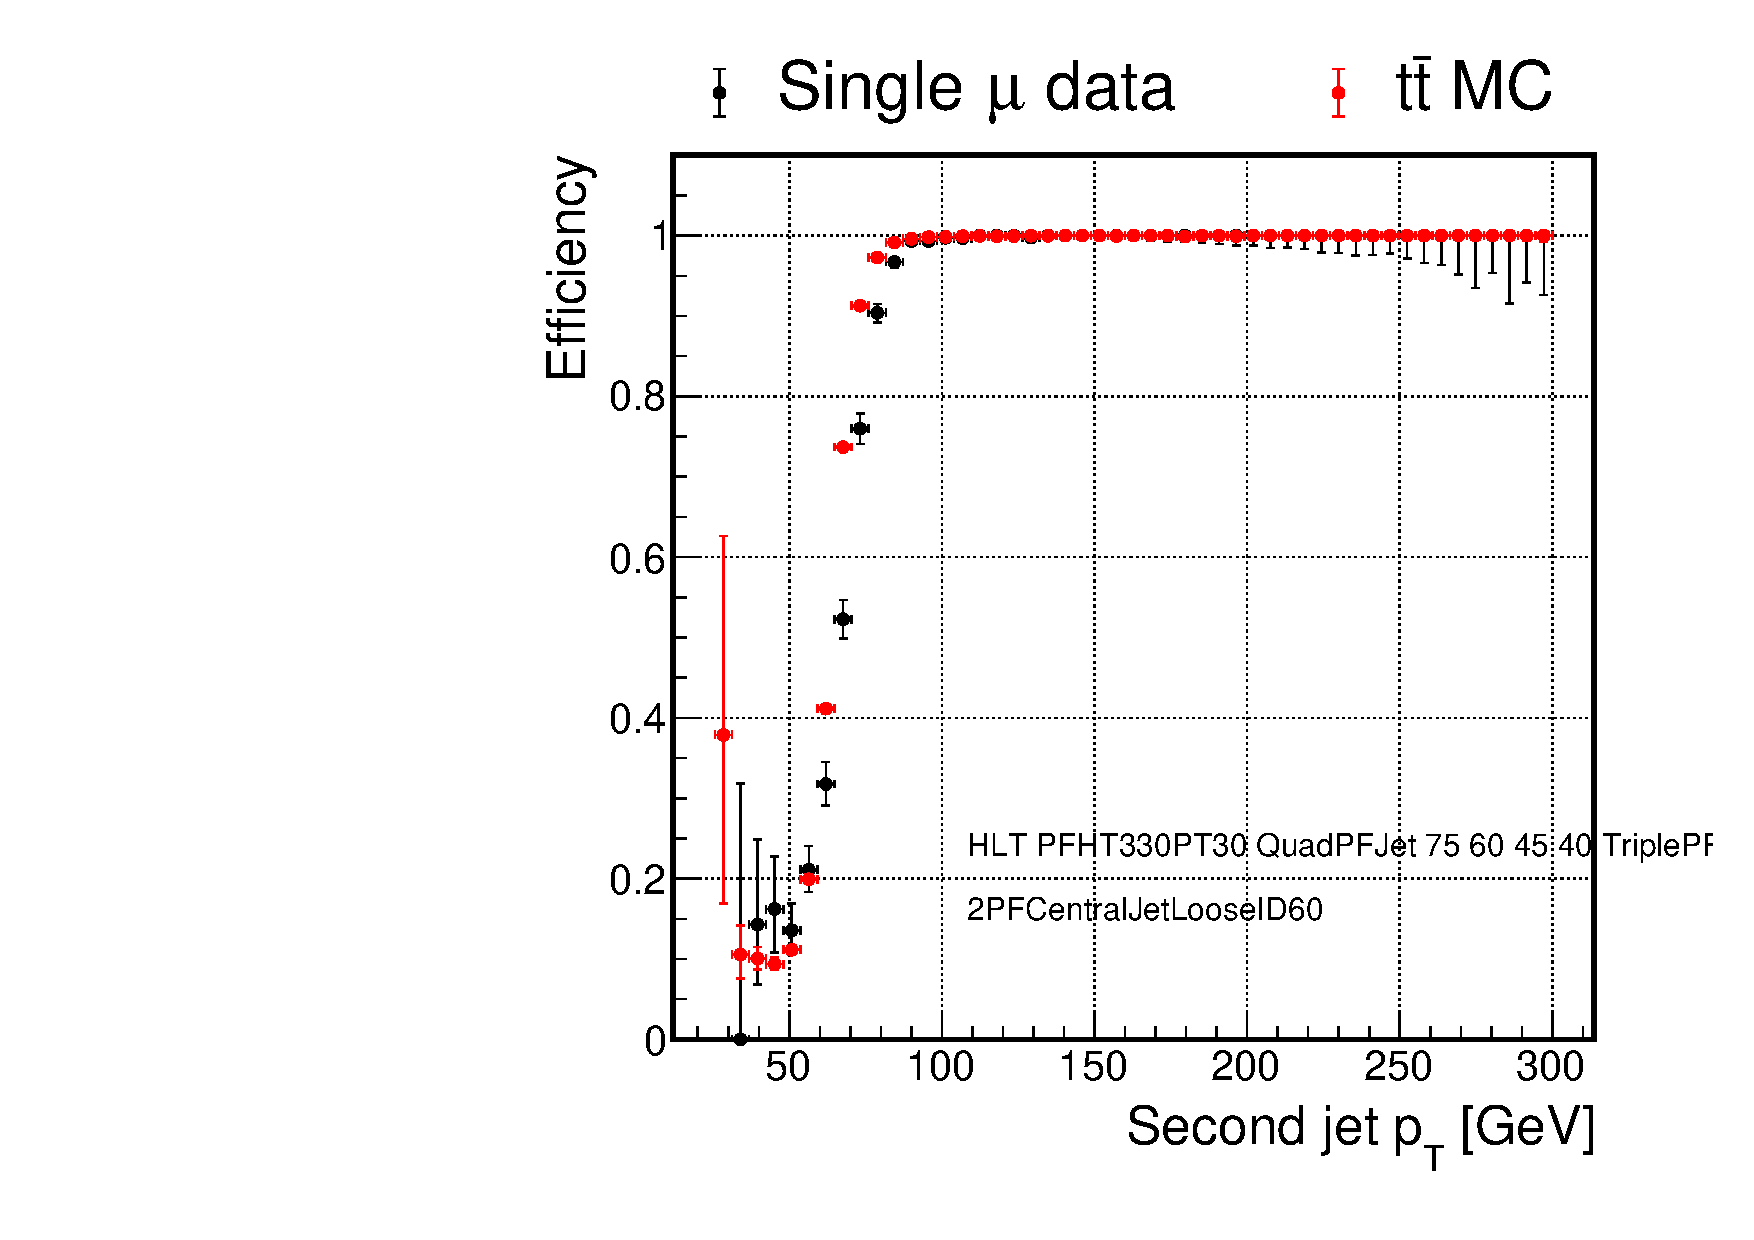
\includegraphics[width=0.3\textwidth]{Figures/AnalysisStrategy/triggereff/plots_2018/Quad_75_60_45_40_3b_Efficiency_2PFCentralJetLooseID60.pdf}}
\subfloat{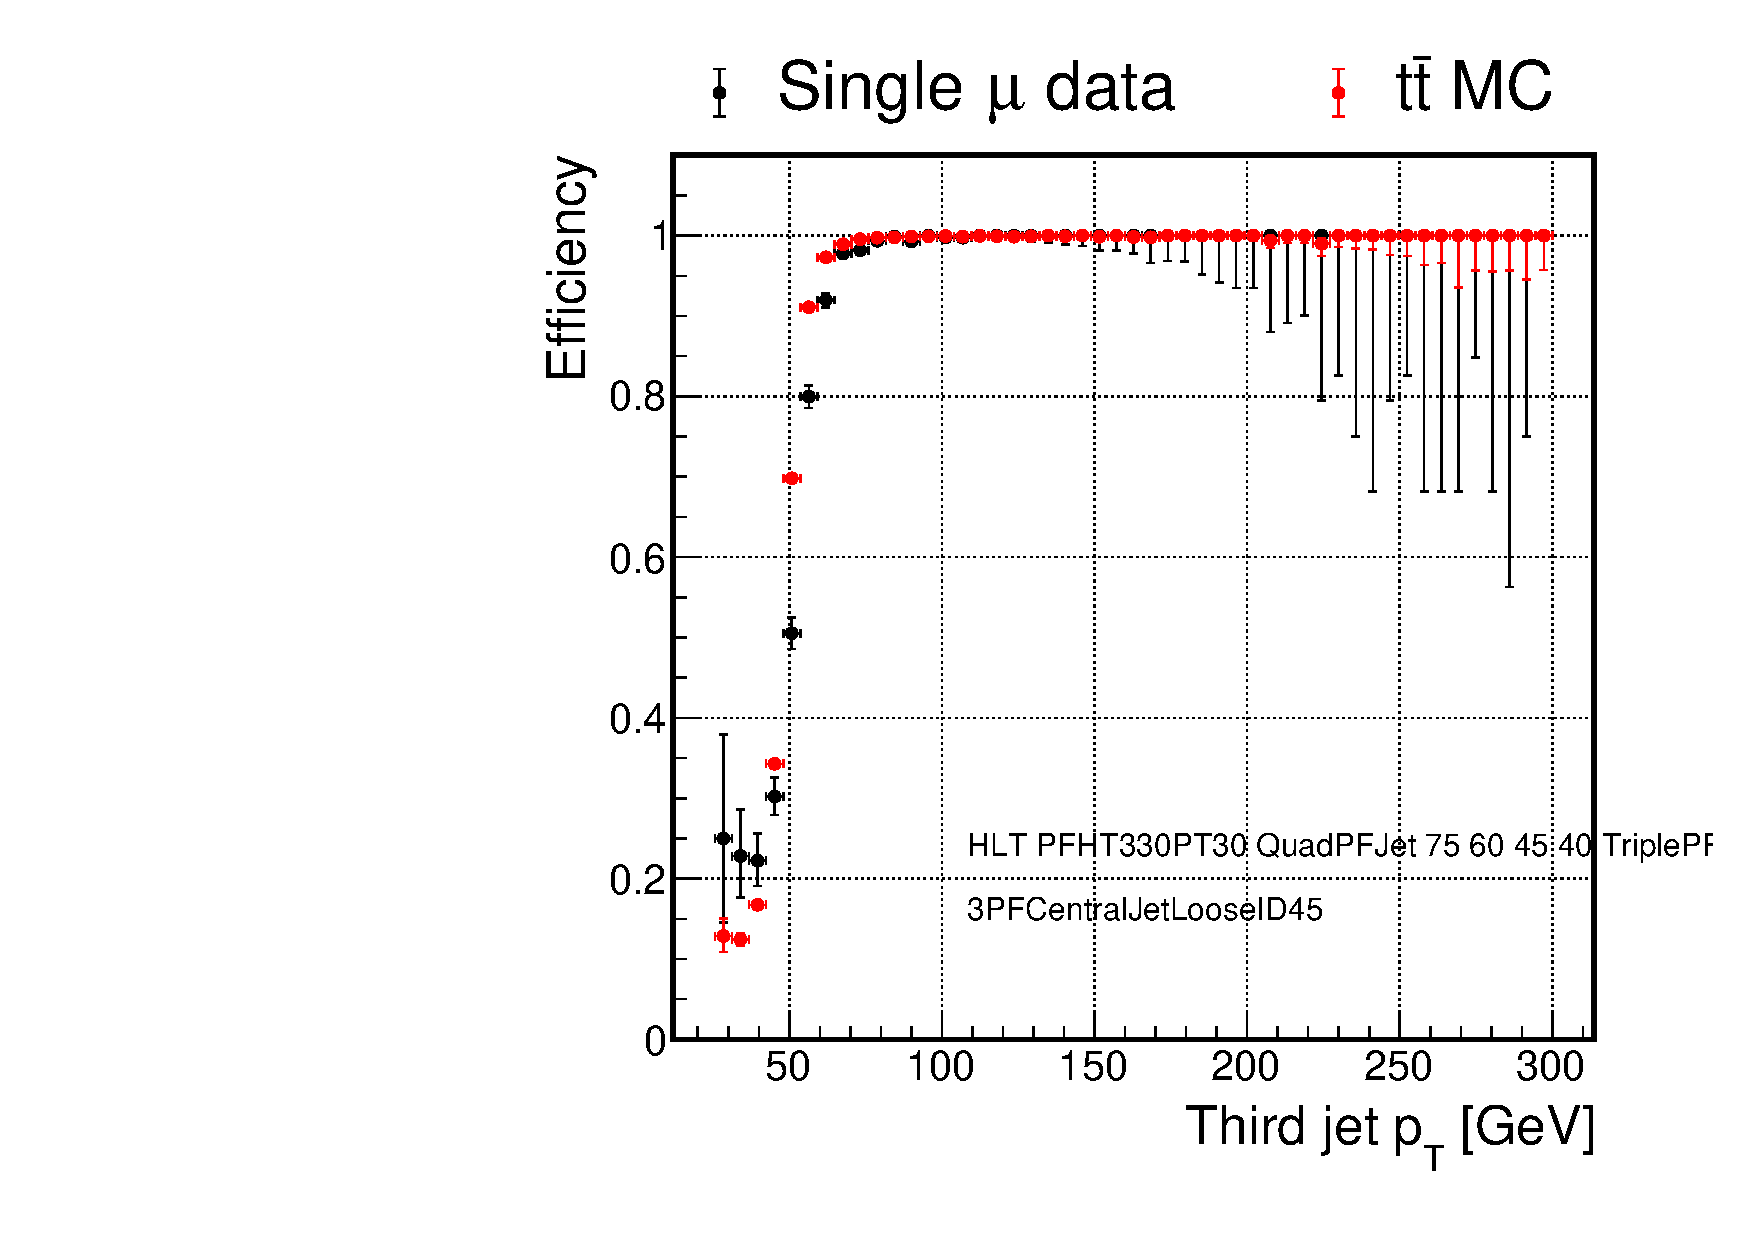
\includegraphics[width=0.3\textwidth]{Figures/AnalysisStrategy/triggereff/plots_2018/Quad_75_60_45_40_3b_Efficiency_3PFCentralJetLooseID45.pdf}}
\subfloat{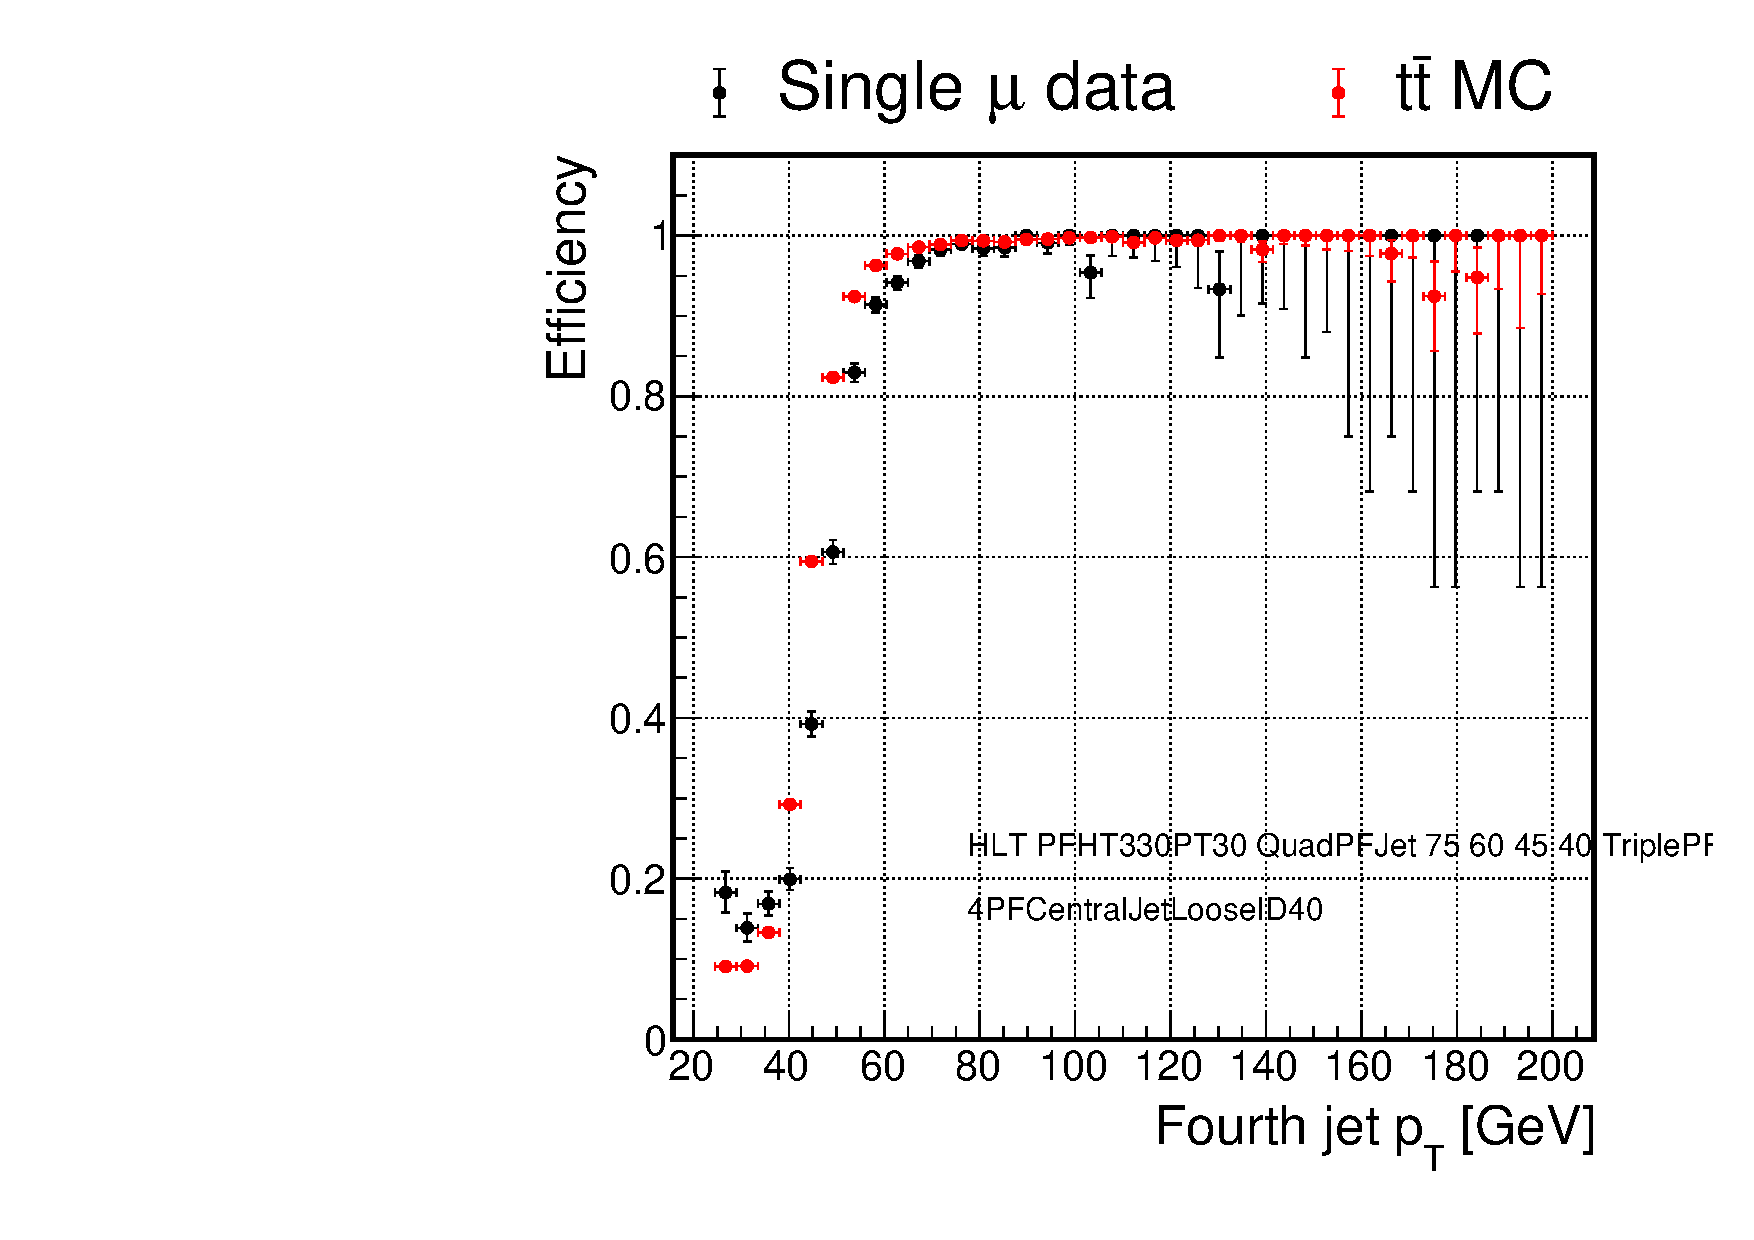
\includegraphics[width=0.3\textwidth]{Figures/AnalysisStrategy/triggereff/plots_2018/Quad_75_60_45_40_3b_Efficiency_4PFCentralJetLooseID40.pdf}}\\
\subfloat{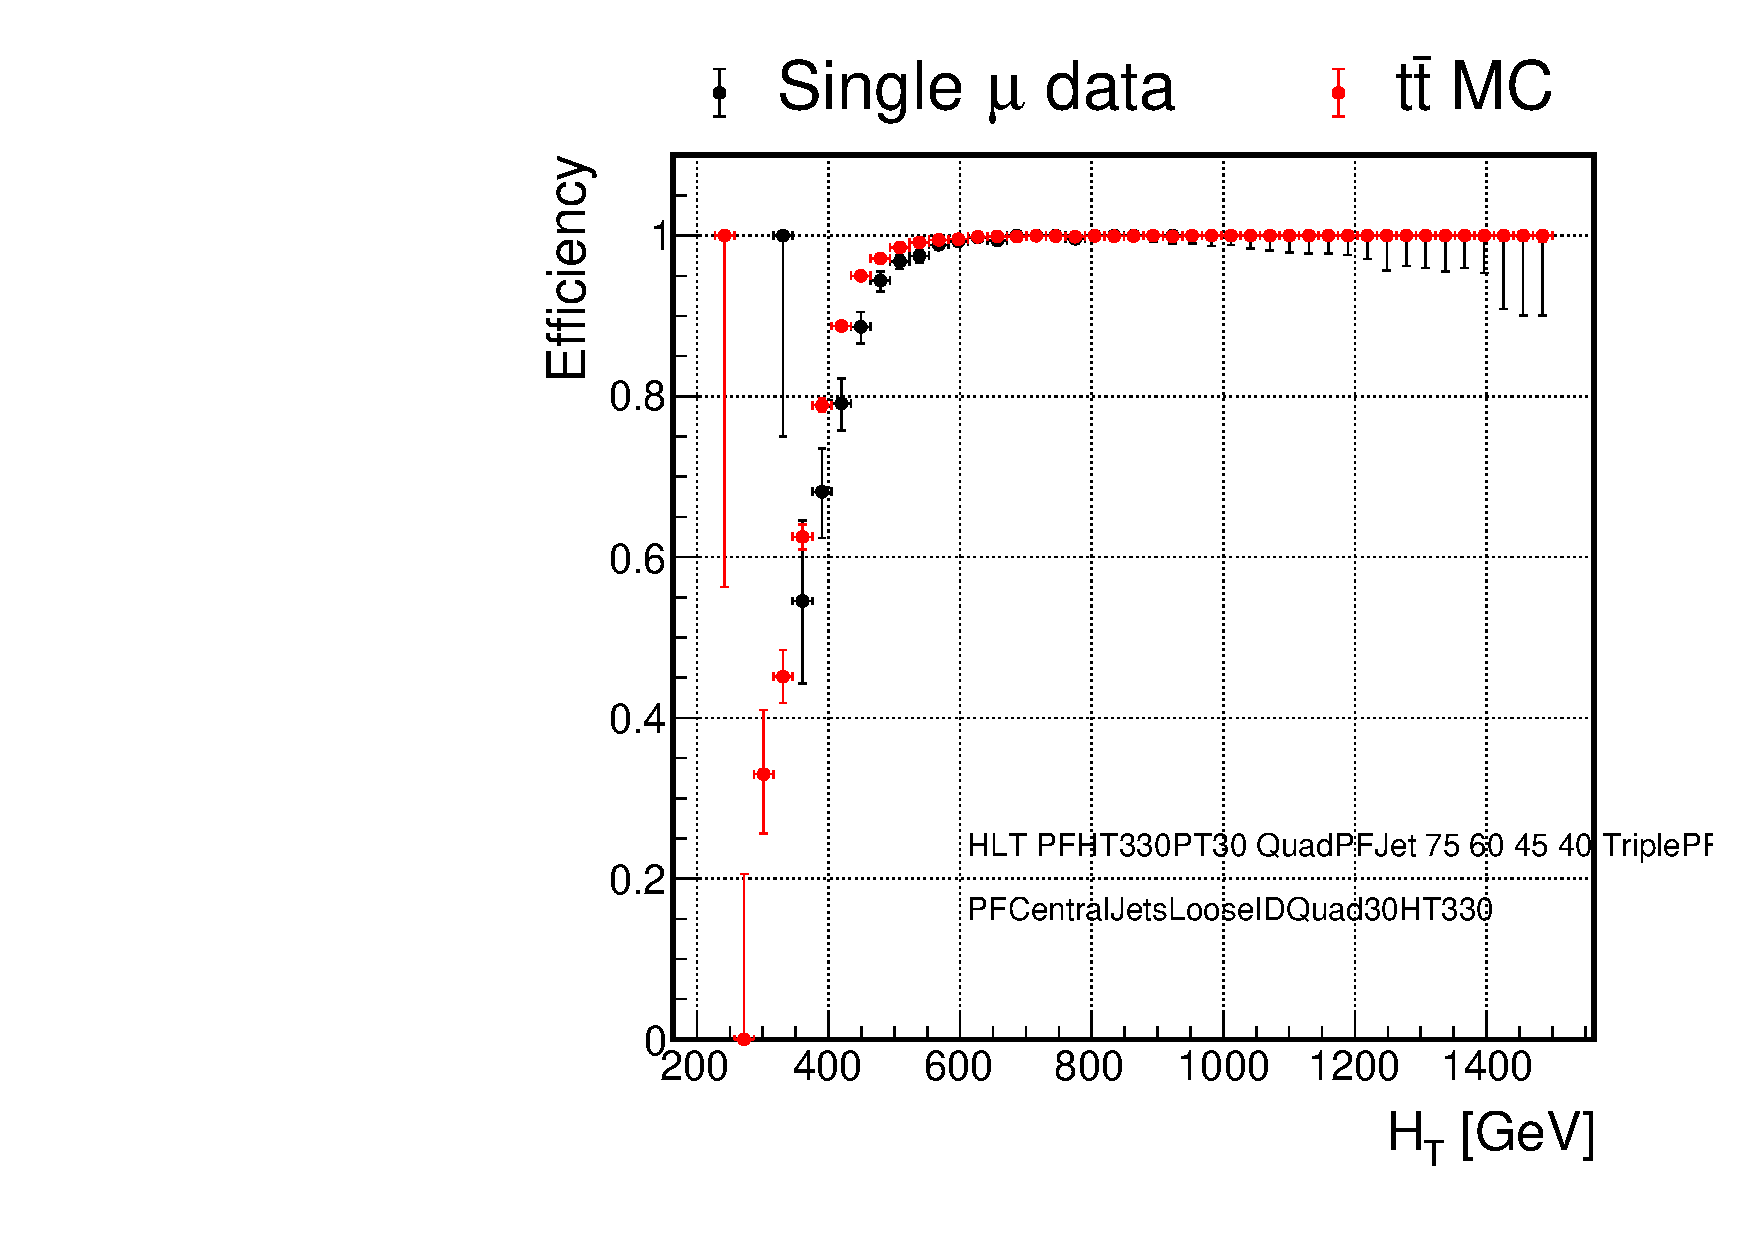
\includegraphics[width=0.3\textwidth]{Figures/AnalysisStrategy/triggereff/plots_2018/Quad_75_60_45_40_3b_Efficiency_PFCentralJetsLooseIDQuad30HT330.pdf}}
\subfloat{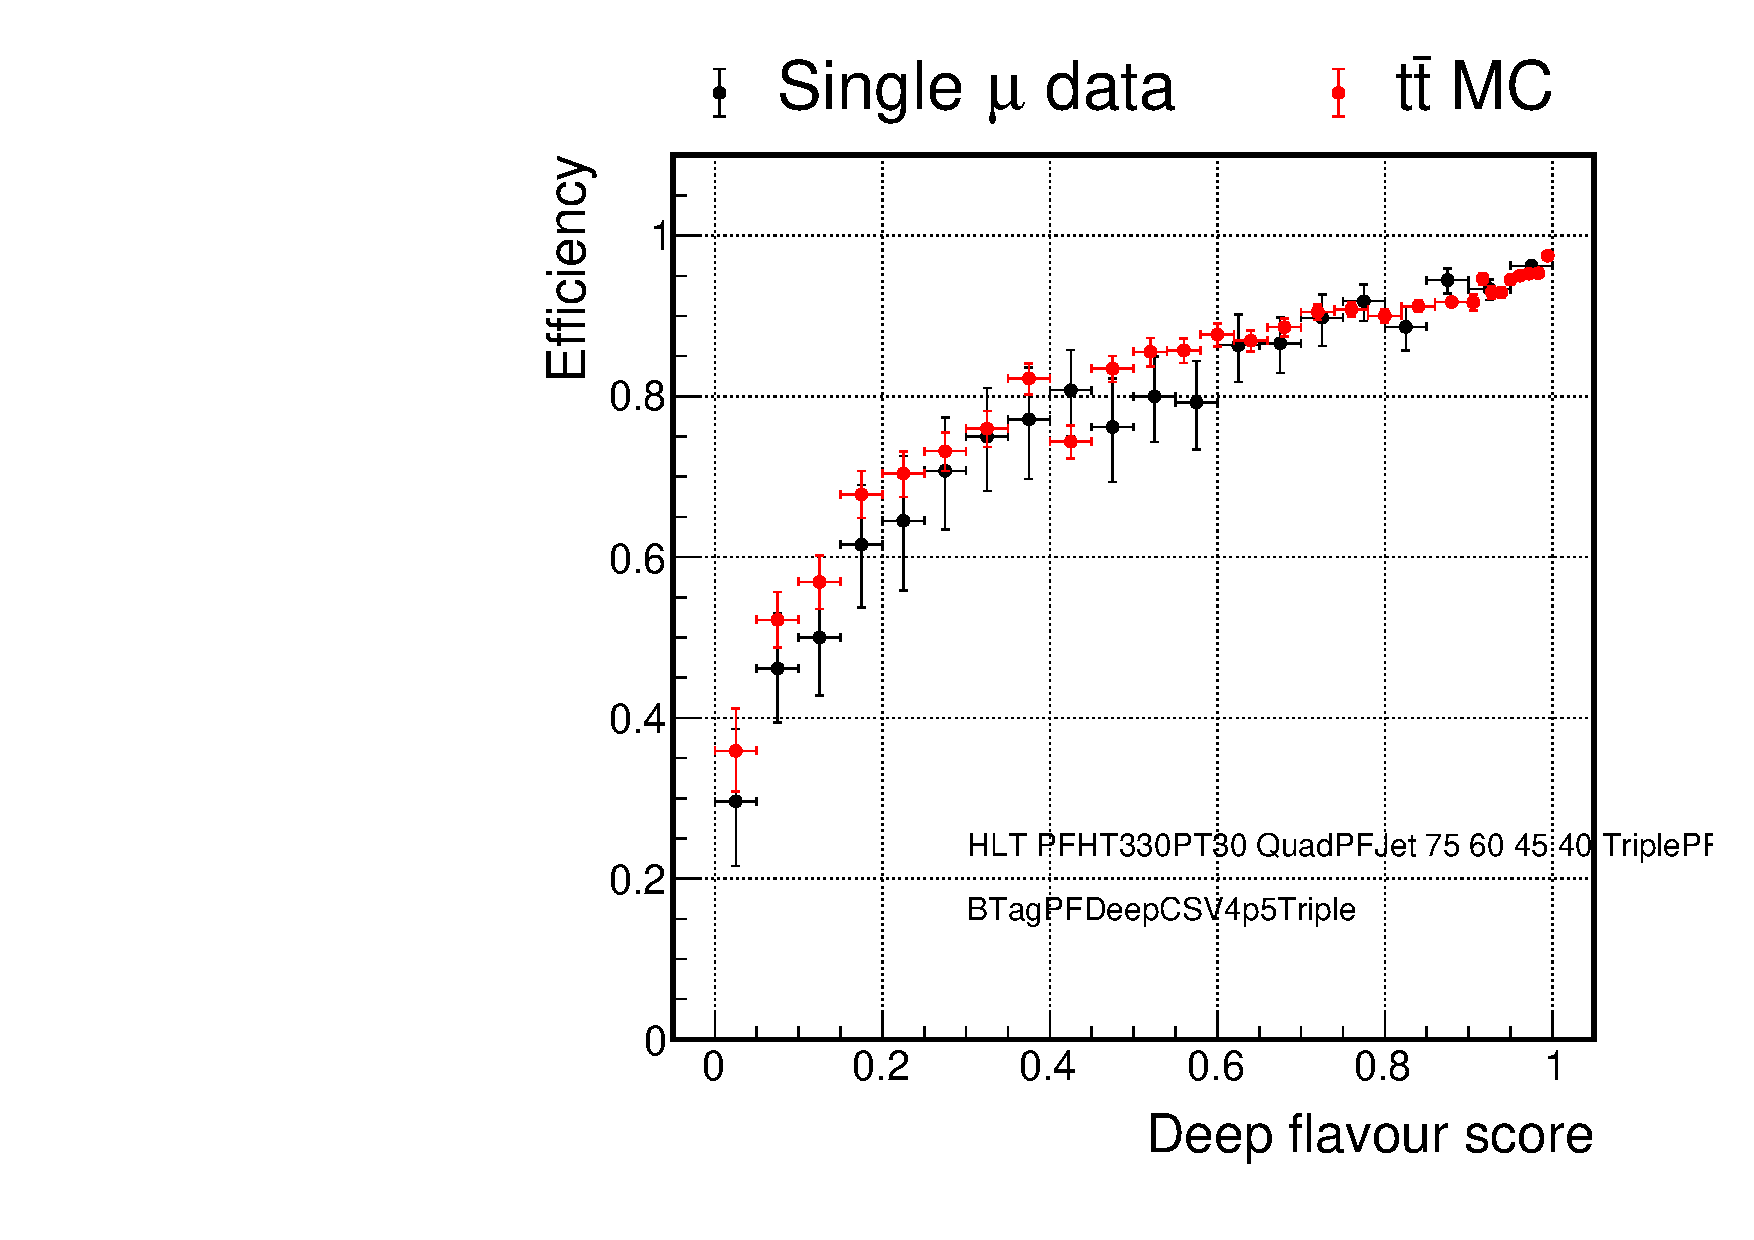
\includegraphics[width=0.3\textwidth]{Figures/AnalysisStrategy/triggereff/plots_2018/Quad_75_60_45_40_3b_Efficiency_BTagPFDeepCSV4p5Triple.pdf}}
\caption[Efficiency measured in single muon data and $\ttbar$ MC for filters of the HLT\_PFHT330PT30\_QuadPFJet\_75\_60\_45\_40\_TriplePFBTagDeepCSV path in 2018]{Efficiency measured in single muon data (black) and $\ttbar$ MC (red) for filters of HLT\_PFHT330PT30\_QuadPFJet\_75\_60\_45\_40\_TriplePFBTagDeepCSV, corresponding to the 2018 dataset.}
\label{trigger:fig:filterEfficiency2018}
\end{figure}


\begin{figure}[htbp!]
\begin{center}
    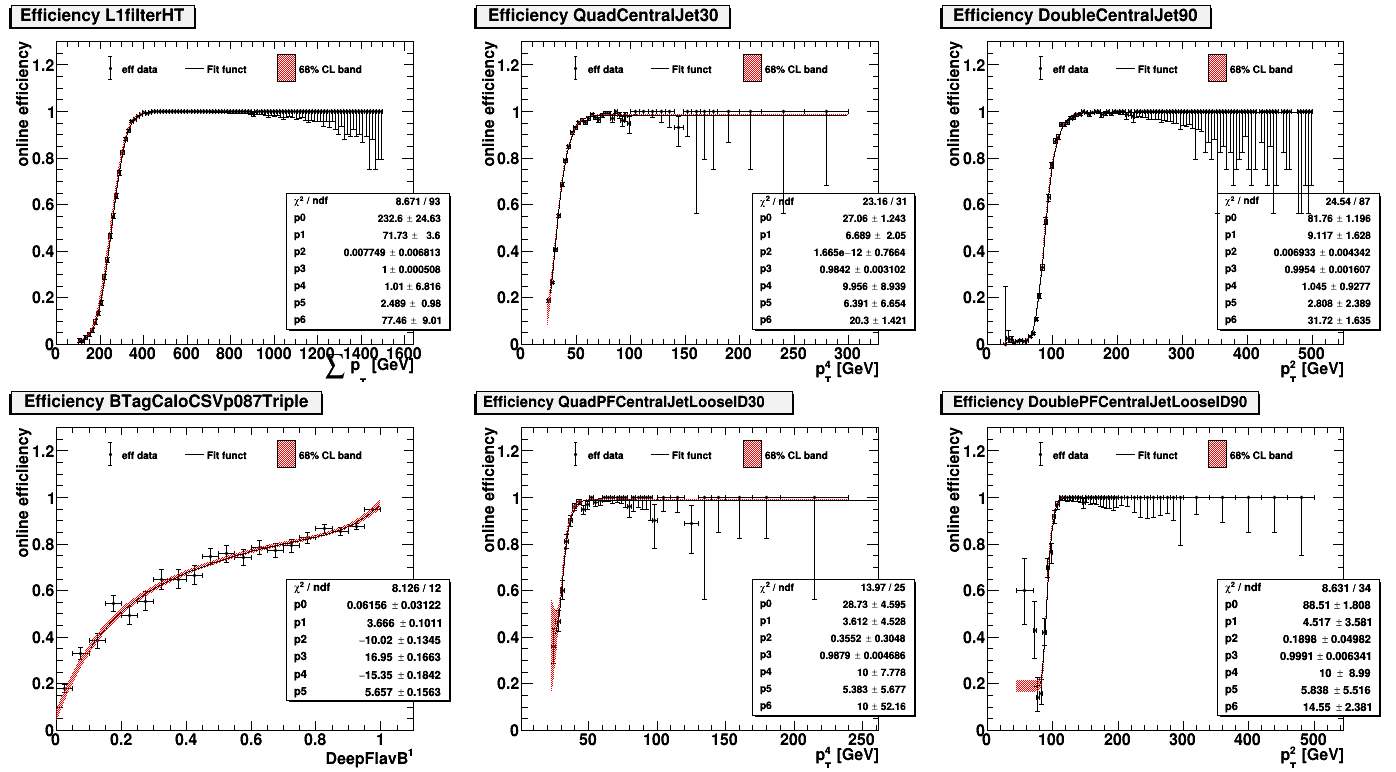
\includegraphics[width=0.9\linewidth]{Figures/AnalysisStrategy/triggerfits/TriggerEfficiencies_2016_TTBarCut_SingleMuon_Double90Quad30_Fit_fullRange.png}
\end{center}
\caption[Efficiency fits in SingleMuon filters of HLT\_DoubleJet90\_Double30\_TripleBTagCSV in 2016]{Efficiency fits in SingleMuon filters of HLT\_DoubleJet90\_Double30\_TripleBTagCSV in 2016. The red band represents the 1 sigma error on the fit obtained from the fit parameter error propagation.}
\label{trigger:fig:SingleMuonFilterEfficiency2016DoubleFit}
\end{figure}

\begin{figure}[htbp!]
\begin{center}
    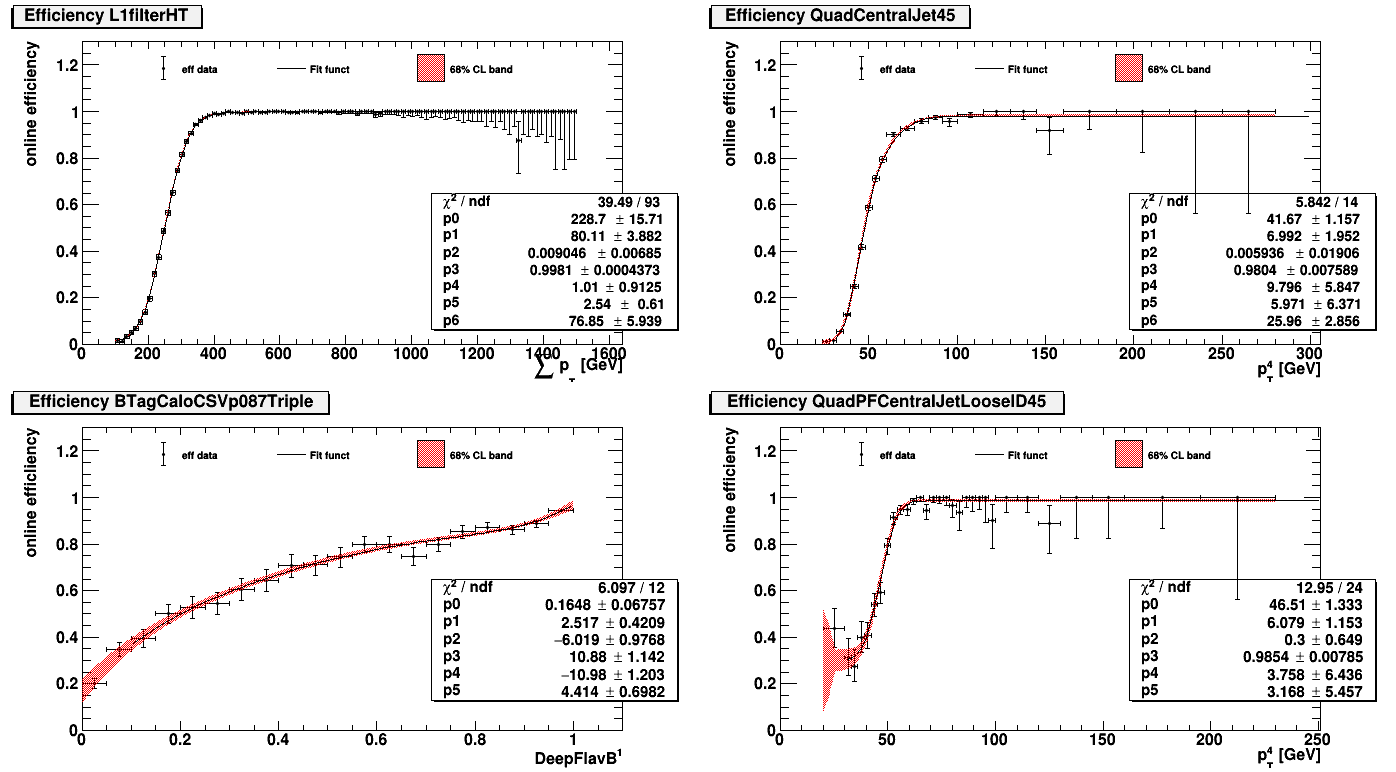
\includegraphics[width=0.9\linewidth]{Figures/AnalysisStrategy/triggerfits/TriggerEfficiencies_2016_TTBarCut_SingleMuon_Quad45_Fit_fullRange.png}
\end{center}
\caption[Efficiency fits in SingleMuon for filters of HLT\_QuadJet45\_TripleBTagCSV in 2016]{Efficiency fits in SingleMuon for filters of HLT\_QuadJet45\_TripleBTagCSV in 2016. The red band represents the 1 sigma error on the fit obtained from the fit parameter error propagation.}
\label{trigger:fig:SingleMuonFilterEfficiency2016QuadFit}
\end{figure}

\begin{figure}[htbp!]
\begin{center}
    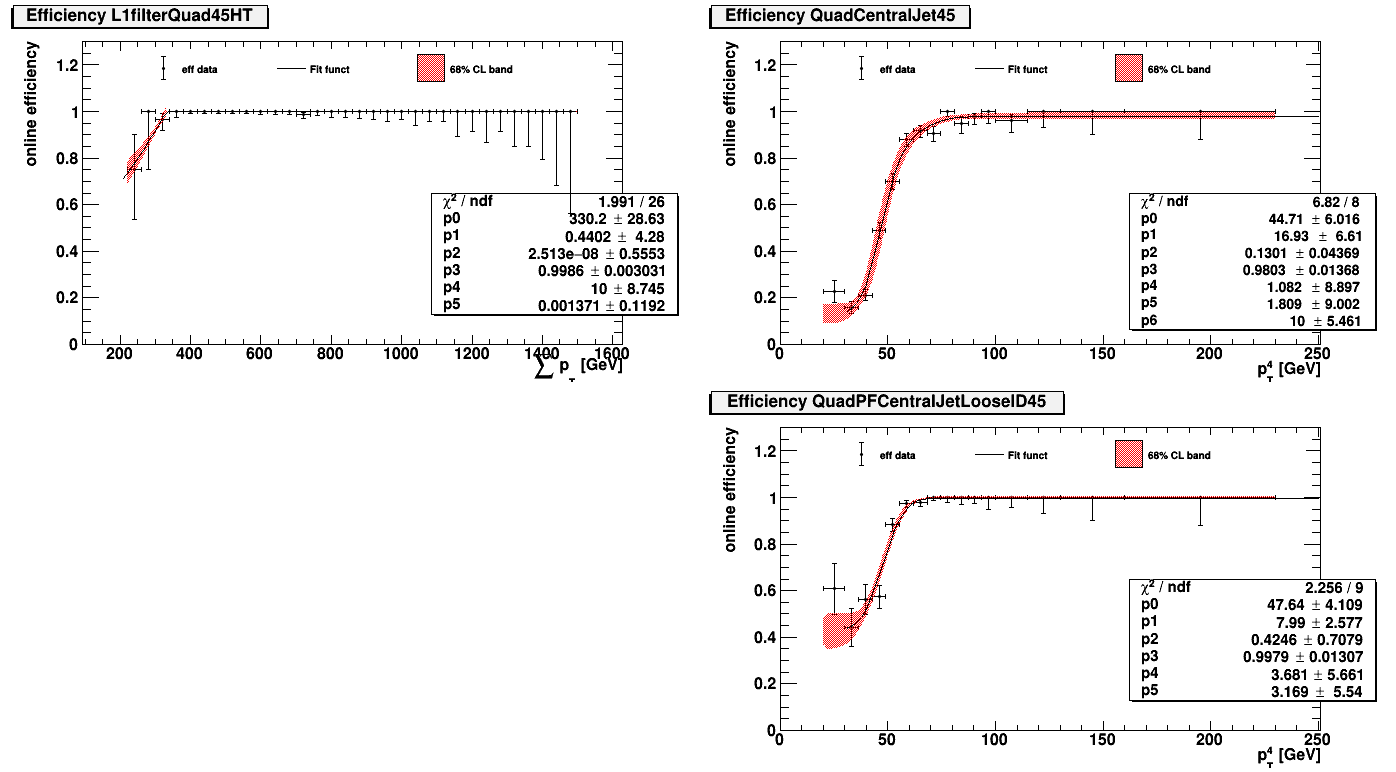
\includegraphics[width=0.9\linewidth]{Figures/AnalysisStrategy/triggerfits/TriggerEfficiencies_2016_TTBarCut_SingleMuon_And_Fit_fullRange.png}
\end{center}
\caption[Efficiency fits in SingleMuon for filters in paths overlap in 2016]{Efficiency fits in SingleMuon for filters of HLT\_QuadJet45\_TripleBTagCSV evaluated over a sample of events passing HLT\_DoubleJet90\_Double30\_TripleBTagCSV in 2016. The red band represents the 1 sigma error on the fit obtained from the fit parameter error propagation.}
\label{trigger:fig:SingleMuonFilterEfficiency2016AndFit}
\end{figure}
    
\begin{figure}[htbp!]
\begin{center}
    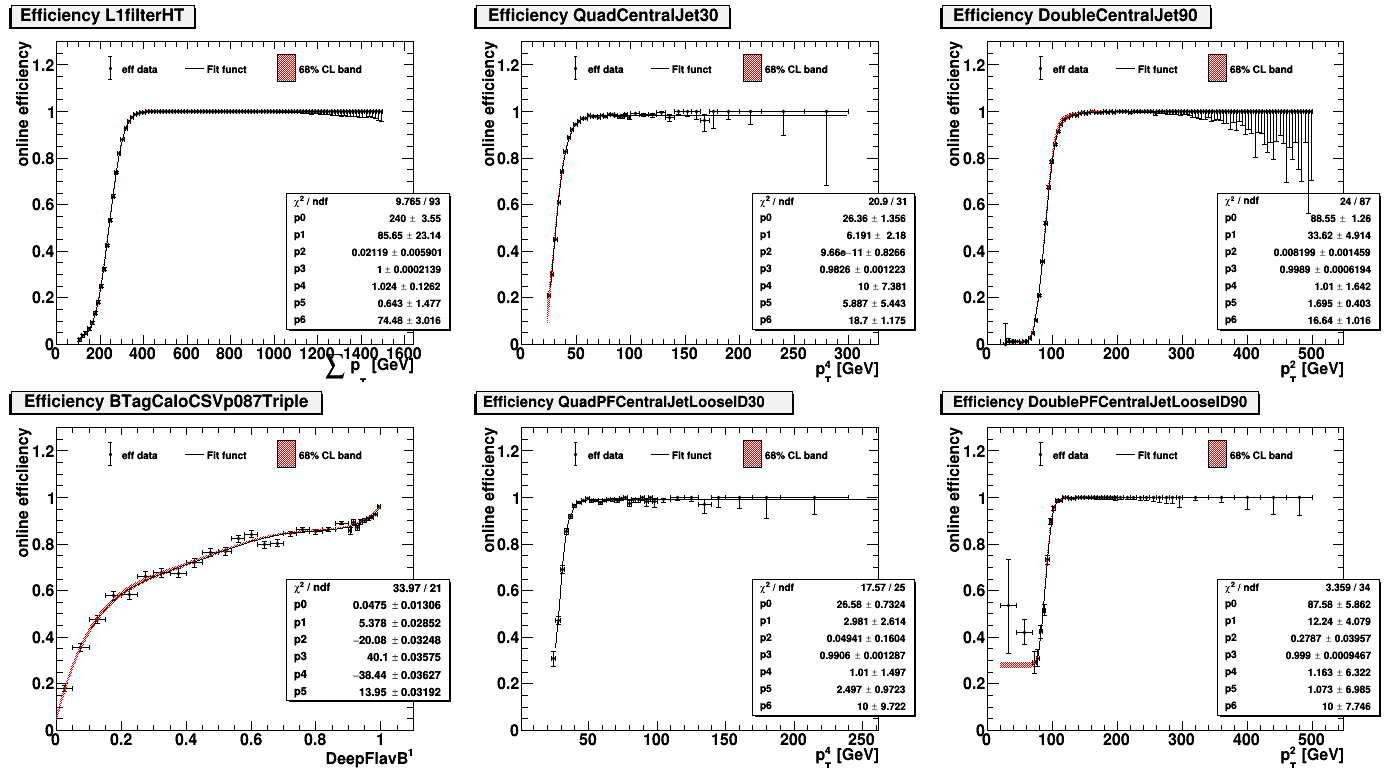
\includegraphics[width=0.9\linewidth]{Figures/AnalysisStrategy/triggerfits/TriggerEfficiencies_2016_TTBarCut_TTbar_Double90Quad30_Fit_fullRange.png}
\end{center}
\caption[Efficiency fits in $\ttbar$ for filters of HLT\_DoubleJet90\_Double30\_TripleBTagCSV in 2016]{Efficiency fits in $\ttbar$ for filters of HLT\_DoubleJet90\_Double30\_TripleBTagCSV in 2016. The red band represents the 1 sigma error on the fit obtained from the fit parameter error propagation.}
\label{trigger:fig:TTbarFilterEfficiency2016DoubleFit}
\end{figure}

\begin{figure}[htbp!]
\begin{center}
    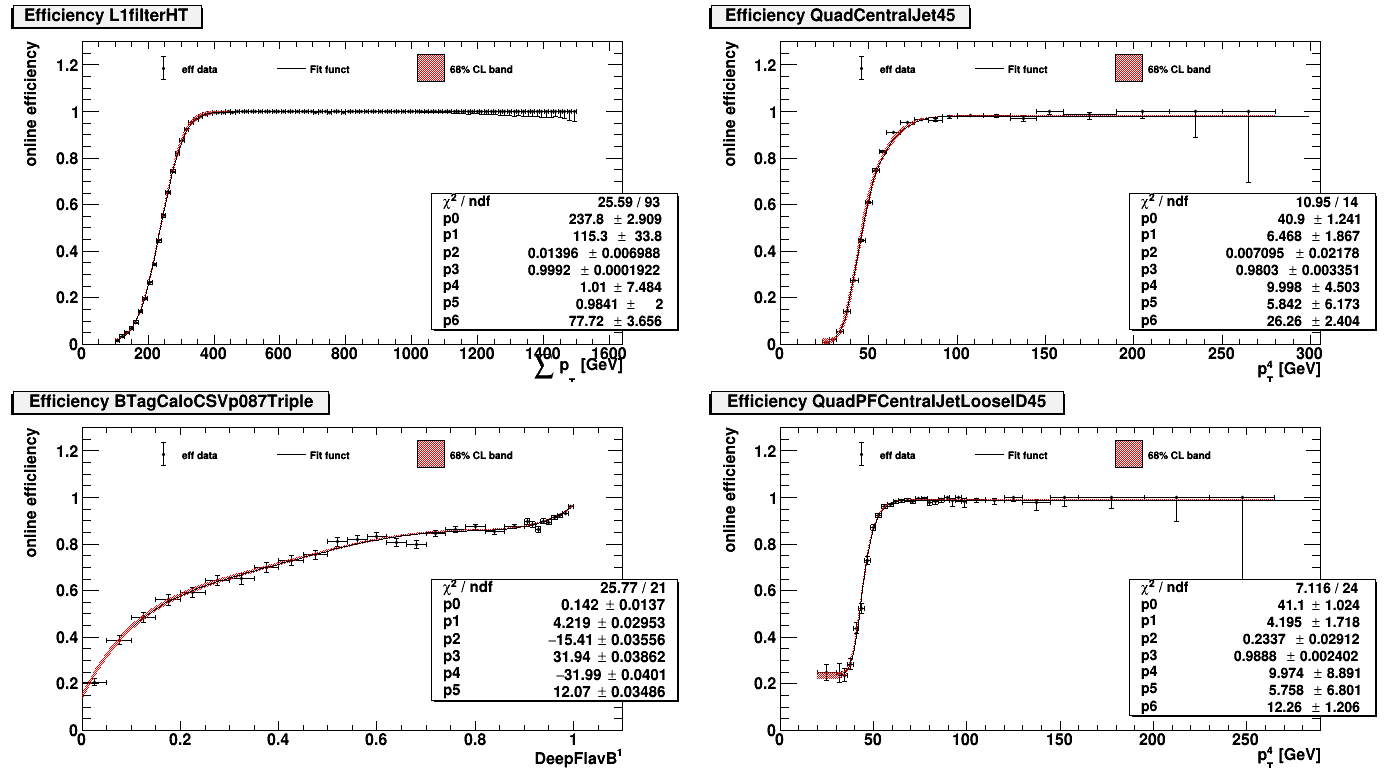
\includegraphics[width=0.8\linewidth]{Figures/AnalysisStrategy/triggerfits/TriggerEfficiencies_2016_TTBarCut_TTbar_Quad45_Fit_fullRange.png}
\end{center}
\caption[Efficiency fits in $\ttbar$ for filters of HLT\_QuadJet45\_TripleBTagCSV in 2016]{Efficiency fits in $\ttbar$ for filters of HLT\_QuadJet45\_TripleBTagCSV in 2016. The red band represents the 1 sigma error on the fit obtained from the fit parameter error propagation.}
\label{trigger:fig:TTbarFilterEfficiency2016QuadFit}
\end{figure}

\begin{figure}[htbp!]
\begin{center}
    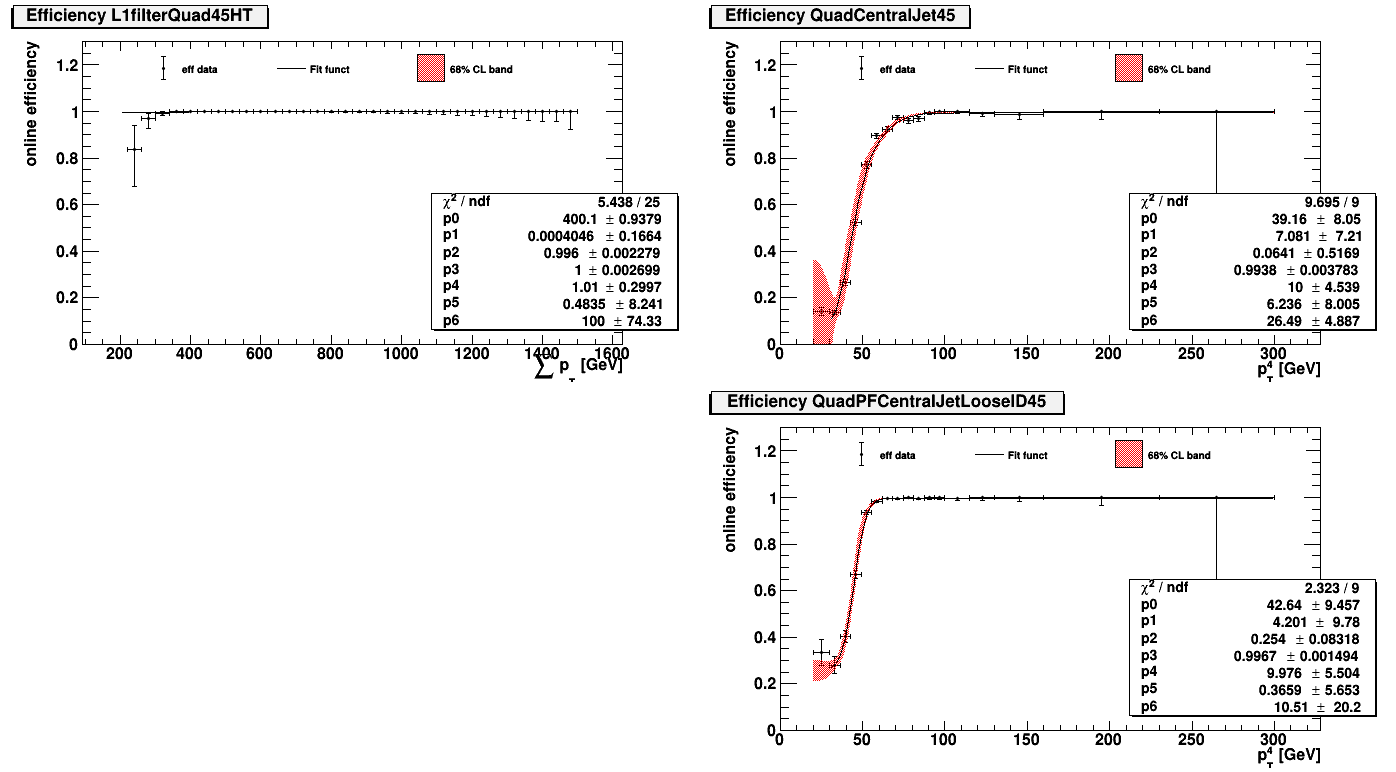
\includegraphics[width=0.8\linewidth]{Figures/AnalysisStrategy/triggerfits/TriggerEfficiencies_2016_TTBarCut_TTbar_And_Fit_fullRange.png}
\end{center}
\caption[Efficiency fits in $\ttbar$ for filters in paths overlap in 2016]{Efficiency fits in $\ttbar$ for filters of HLT\_QuadJet45\_TripleBTagCSV evaluated over a sample of events passing HLT\_DoubleJet90\_Double30\_TripleBTagCSV in 2016. The red band represents the 1 sigma error on the fit obtained from the fit parameter error propagation. Due to the limited statistic of the first two bins, the fit is not able to model the turn-on curve, however it was verified that this does not cause a problem in the model thanks to the closure test in 2016 signal.}
\label{trigger:fig:TTbarFilterEfficiency2016AndFit}
\end{figure}

%%%%%%%%%%%%%%%%%%%%%% 2017 trigger fits
\begin{figure}[htbp!]
\begin{center}
    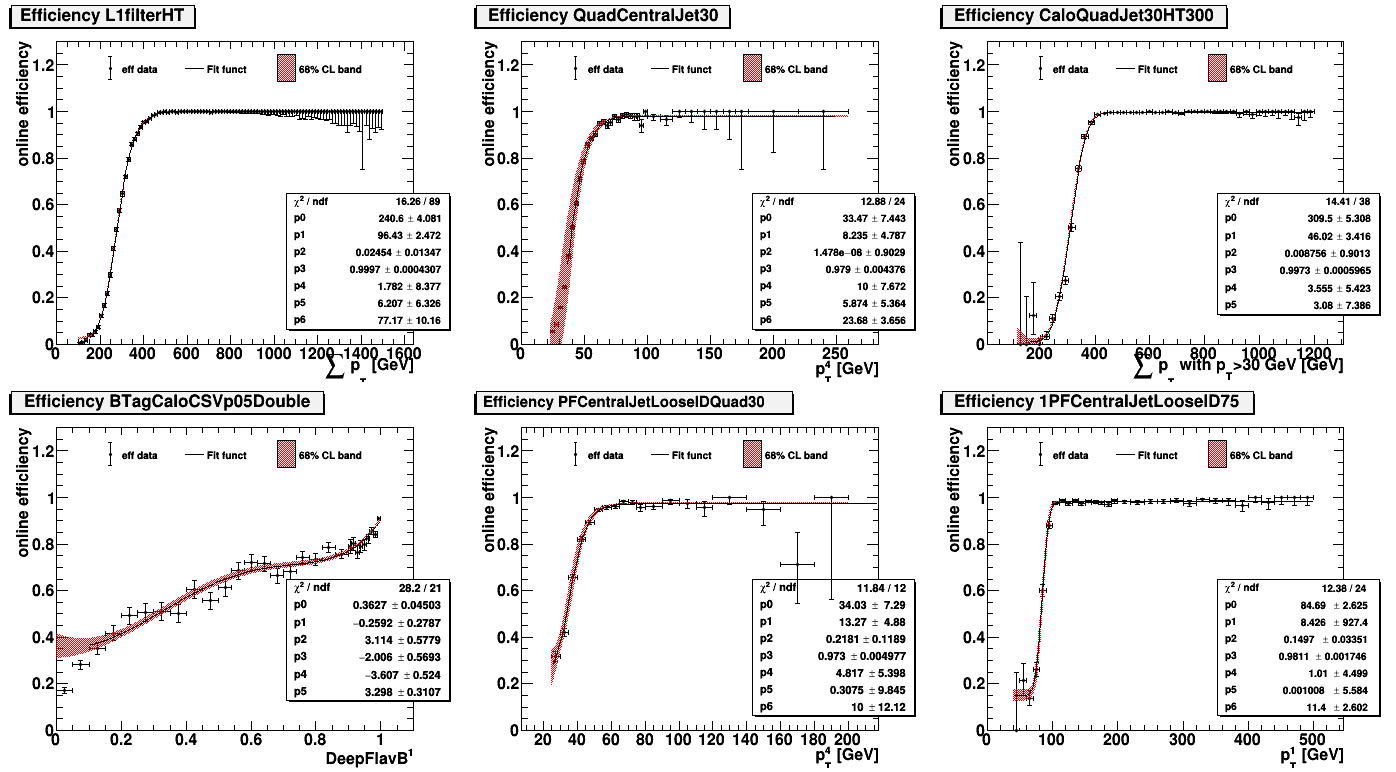
\includegraphics[width=0.9\linewidth]{Figures/AnalysisStrategy/triggerfits/TriggerEfficiencies_2017_TTBarCut_SingleMuon_2017_1_Fit.png}
\end{center}
\caption[Efficiency fits in SingleMuon for filters of the trigger path in 2017 (1/2)]{Efficiency fits in SingleMuon for filters of the trigger path in 2017 (1/2). The red band represents the 1 sigma error on the fit obtained from the fit parameter error propagation.}
\label{trigger:fig:SingleMuonFilterEfficiency2017_1}
\end{figure}

\begin{figure}[htbp!]
\begin{center}
    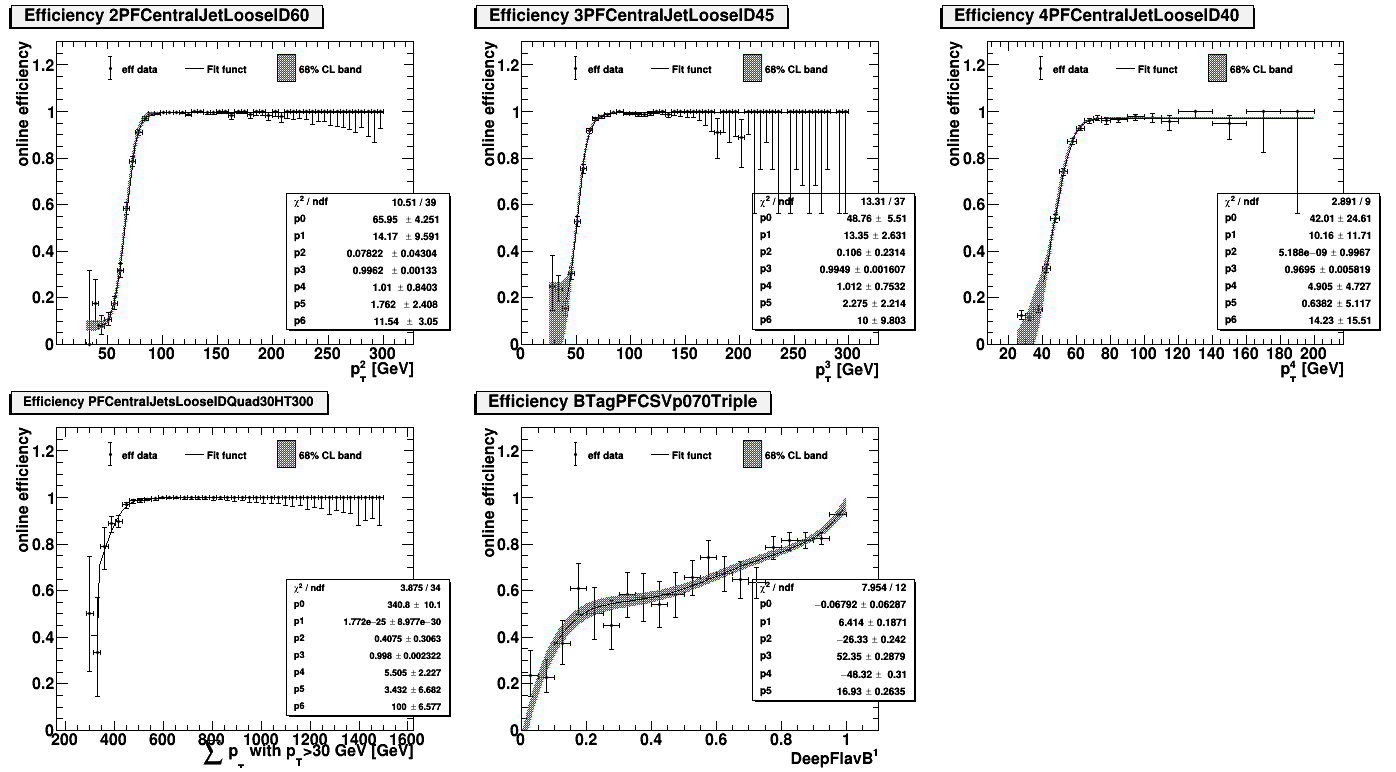
\includegraphics[width=0.9\linewidth]{Figures/AnalysisStrategy/triggerfits/TriggerEfficiencies_2017_TTBarCut_SingleMuon_2017_2_Fit.png}
\end{center}
\caption[Efficiency fits in SingleMuon for filters of the trigger path in 2017 (2/2)]{Efficiency fits in SingleMuon for filters of the trigger path in 2017 (2/2). The red band represents the 1 sigma error on the fit obtained from the fit parameter error propagation.}
\label{trigger:fig:SingleMuonFilterEfficiency2017_2}
\end{figure}
    
\begin{figure}[htbp!]
\begin{center}
    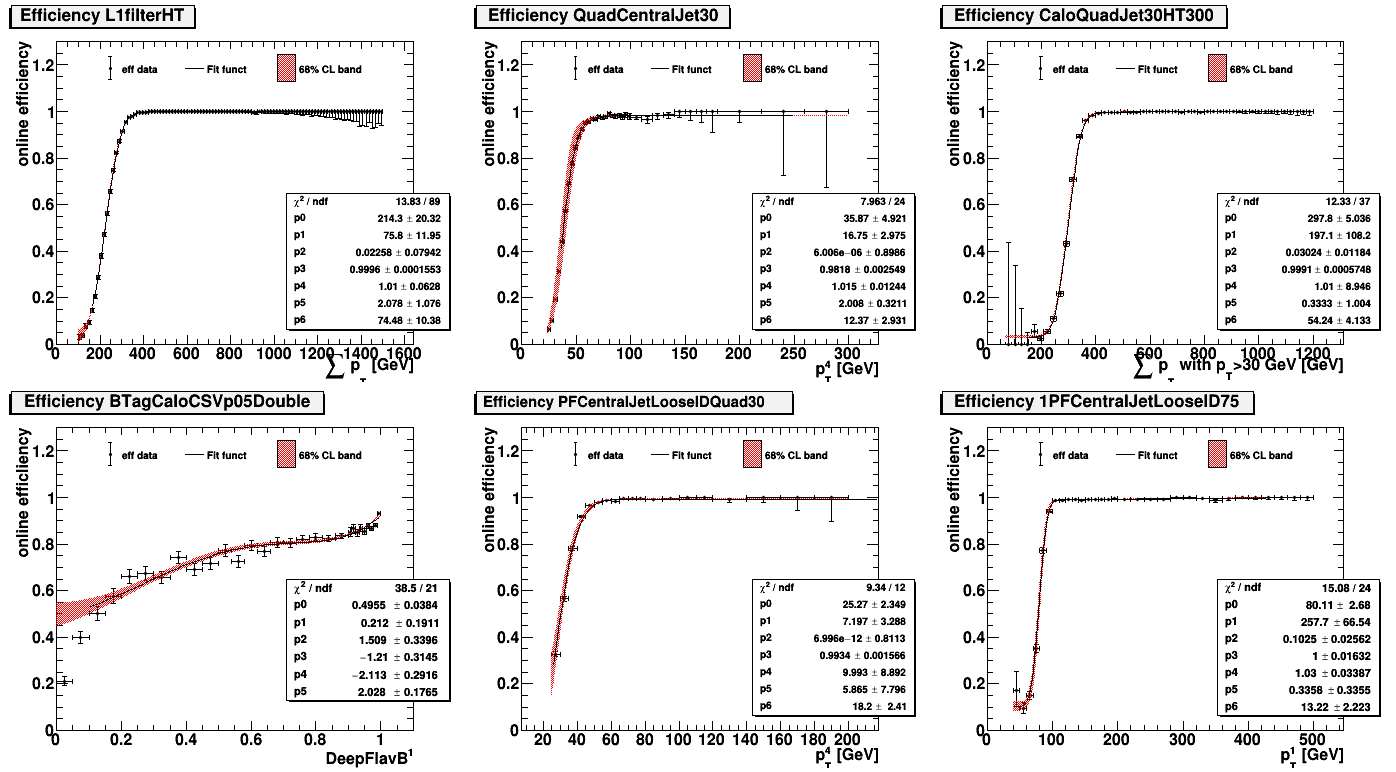
\includegraphics[width=0.9\linewidth]{Figures/AnalysisStrategy/triggerfits/TriggerEfficiencies_2017_TTBarCut_TTbar_2017_1_Fit.png}
\end{center}
\caption[Efficiency fits in $\ttbar$ for filters of the trigger path in 2017 (1/2)]{Efficiency fits in $\ttbar$ for filters of the trigger path in 2017 (1/2). The red band represents the 1 sigma error on the fit obtained from the fit parameter error propagation.}
\label{trigger:fig:TTbarFilterEfficiency2017_1}
\end{figure}
   
\begin{figure}[htbp!]
\begin{center}
    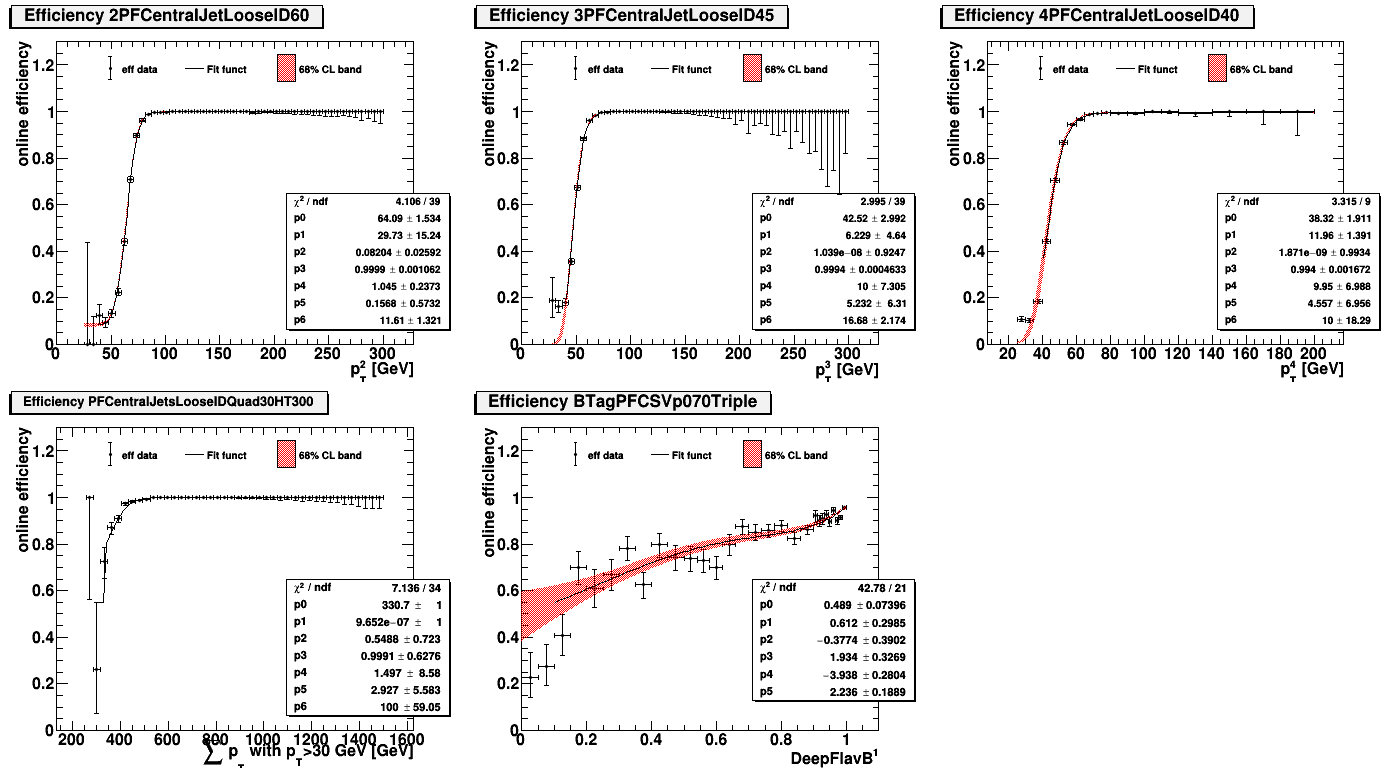
\includegraphics[width=0.9\linewidth]{Figures/AnalysisStrategy/triggerfits/TriggerEfficiencies_2017_TTBarCut_TTbar_2017_2_Fit.png}
\end{center}
\caption[Efficiency fits in $\ttbar$ for filters of the trigger path in 2017 (2/2)]{Efficiency fits in $\ttbar$ for filters of the trigger path in 2017 (2/2). The red band represents the 1 sigma error on the fit obtained from the fit parameter error propagation.}
\label{trigger:fig:TTbarFilterEfficiency2017_2}
\end{figure}

%%%%%%%%%%%%%%%%%%%%%% 2018 fits

\begin{figure}[htbp!]
\begin{center}
    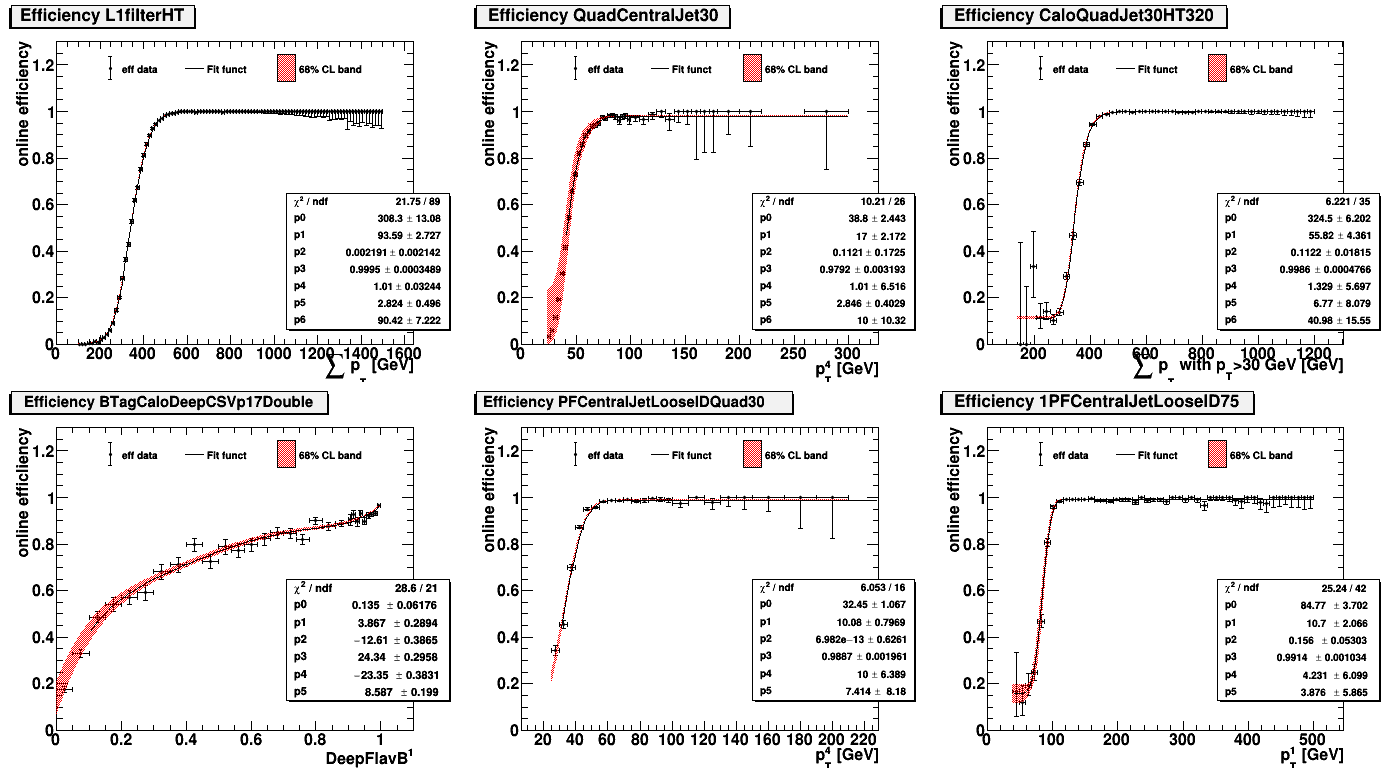
\includegraphics[width=0.9\linewidth]{Figures/AnalysisStrategy/triggerfits/TriggerEfficiencies_2018_TTBarCut_SingleMuon_2018_1_Fit.png}
\end{center}
\caption[Efficiency fits in SingleMuon for filters of the trigger path in 2018 (1/2)]{Efficiency fits in SingleMuon for filters of the trigger path in 2018 (1/2). The red band represents the 1 sigma error on the fit obtained from the fit parameter error propagation.}
\label{trigger:fig:SingleMuonFilterEfficiency2018_1}
\end{figure}

\begin{figure}[htbp!]
\begin{center}
    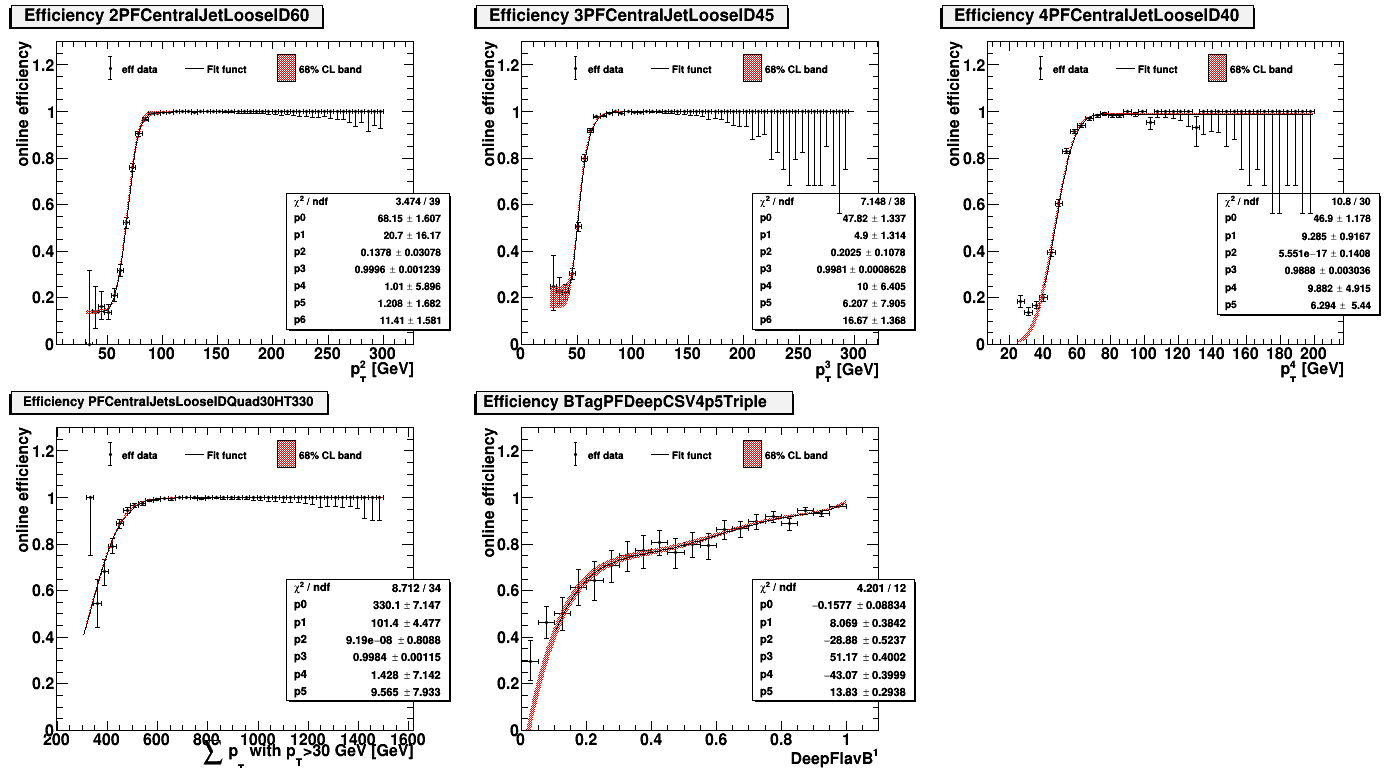
\includegraphics[width=0.9\linewidth]{Figures/AnalysisStrategy/triggerfits/TriggerEfficiencies_2018_TTBarCut_SingleMuon_2018_2_Fit.png}
\end{center}
\caption[Efficiency fits in SingleMuon for filters of the trigger path in 2018 (2/2)]{Efficiency fits in SingleMuon for filters of the trigger path in 2018 (2/2). The red band represents the 1 sigma error on the fit obtained from the fit parameter error propagation.}
\label{trigger:fig:SingleMuonFilterEfficiency2018_2}
\end{figure}
    
\begin{figure}[htbp!]
\begin{center}
    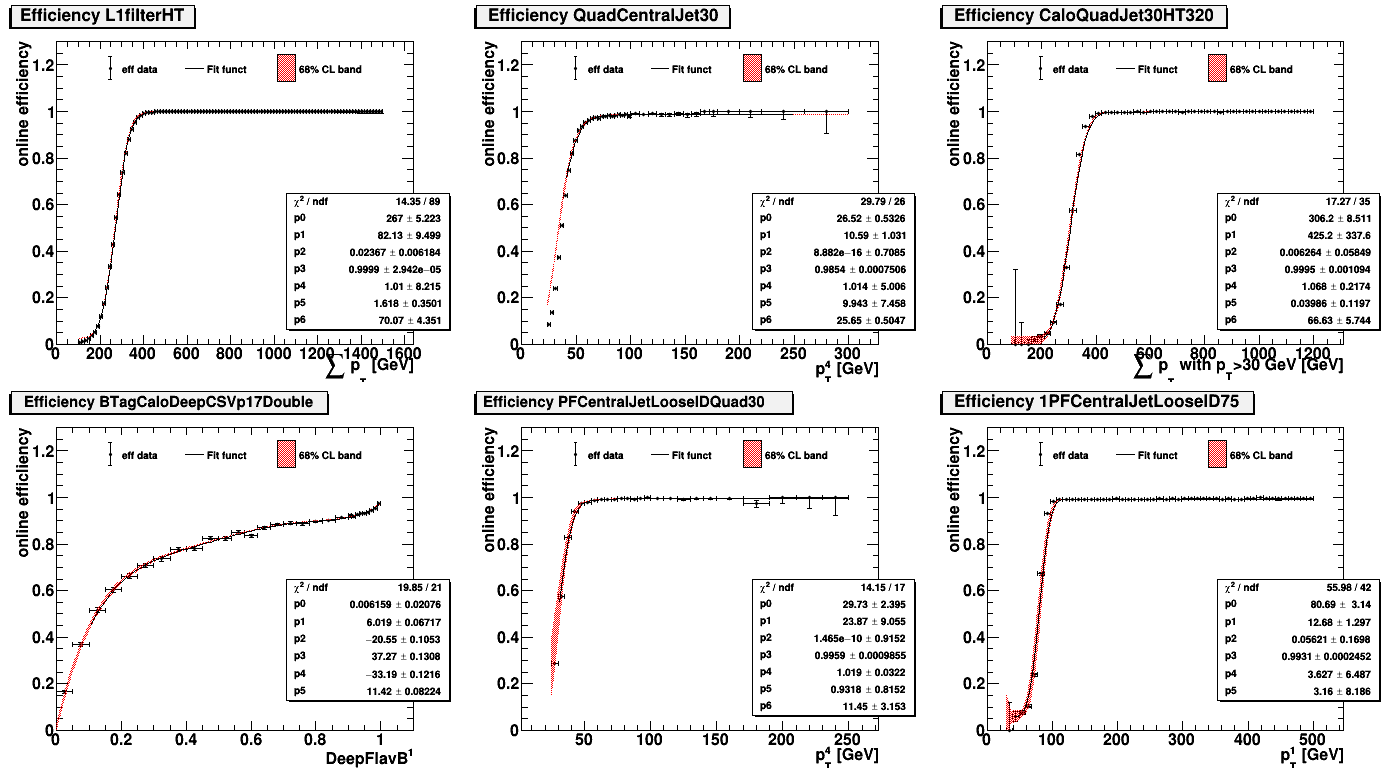
\includegraphics[width=0.9\linewidth]{Figures/AnalysisStrategy/triggerfits/TriggerEfficiencies_2018_TTBarCut_TTbar_2018_1_Fit.png}
\end{center}
\caption[Efficiency fits in $\ttbar$ for filters of the trigger path in 2018 (1/2)]{Efficiency fits in $\ttbar$ for filters of the trigger path in 2018 (1/2). The red band represents the 1 sigma error on the fit obtained from the fit parameter error propagation.}
\label{trigger:fig:TTbarFilterEfficiency2018_1}
\end{figure}
    
\begin{figure}[htbp!]
\begin{center}
    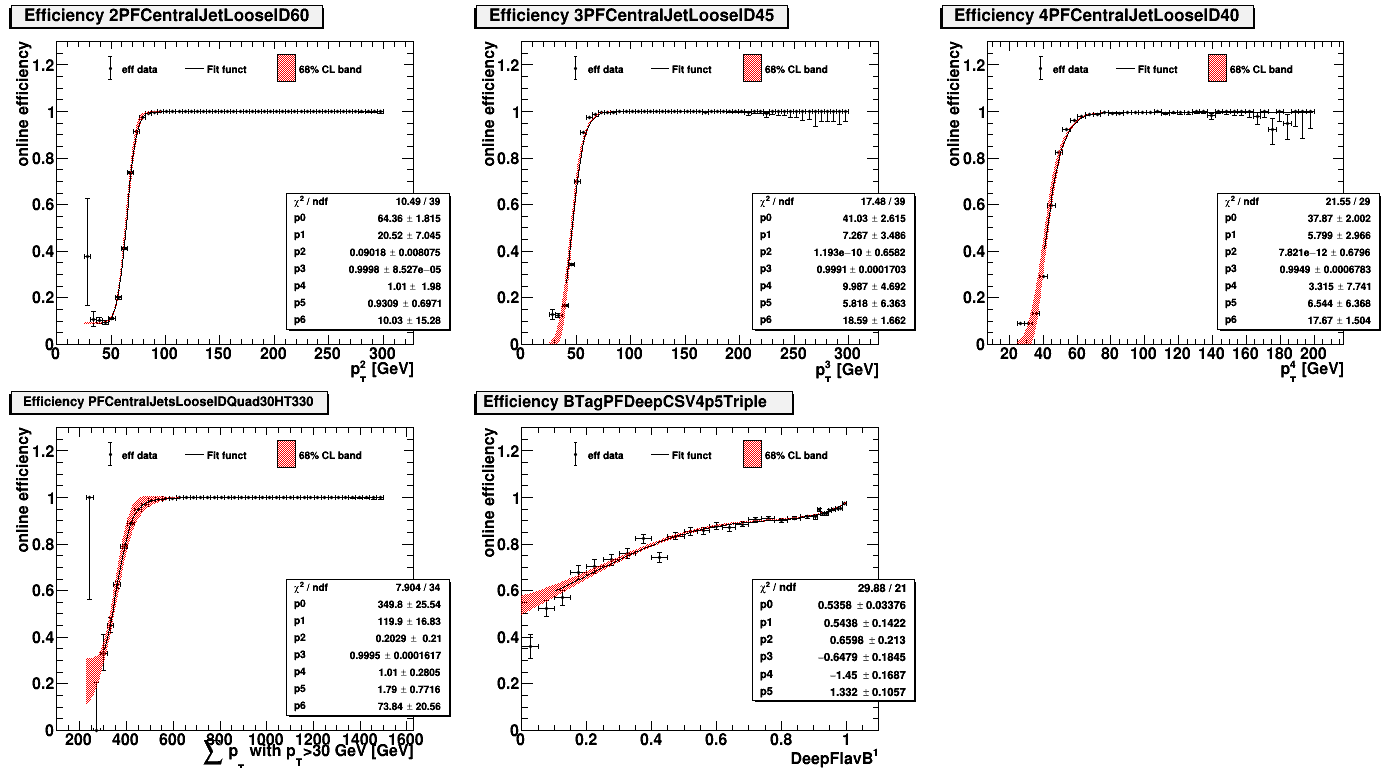
\includegraphics[width=0.9\linewidth]{Figures/AnalysisStrategy/triggerfits/TriggerEfficiencies_2018_TTBarCut_TTbar_2018_2_Fit.png}
\end{center}
\caption[Efficiency fits in $\ttbar$ for filters of the trigger path in 2018 (2/2)]{Efficiency fits in $\ttbar$ for filters of the trigger path in 2018 (2/2). The red band represents the 1 sigma error on the fit obtained from the fit parameter error propagation.}
\label{trigger:fig:TTbarFilterEfficiency2018_2}
\end{figure}

\chapter{ggFKiller score}\label{appendix:ggfkiller}
This appendix describes more details on the ggFKiller training. The simulation events were separated into 75\% training and 25\% test. The ggFKiller chosen hyperparameters for the 2016, 2017 and 2018 dataset are presented in Table~\ref{event_selection:tab:ggfkillerconfig}. For completeness, the distributions of the input variables in signal and background for 2017 and 2018 are presented in Figure~\ref{event_selection:fig:bdtvariables2017}, and Figure~\ref{event_selection:fig:bdtvariables2018}, respectively. The optimization procedure is summarized as follows:
\begin{itemize}
	\setlength\itemsep{0.01em}
	\item Eight grids with 4 points of BDT-hyperparameters each are defined. Each point is a different combination of number of estimators, maximum depth, maximum learning rate
	\item The best of point of each grid is found using a 2-fold cross-validation training performed using the GridSearchCV method implemented in scikit-learn~\cite{scikitlearn}. In essence, the procedure is the following: 1) The training sample is divided in 2 folds, 2) Iteratively one fold is used for training and the remaining one for the validation, 3) The mean of the 2 ROC-AUCs in the validation sample for each point of the grid is calculated. The best point of the grid is the one which maximizes this mean.
\item The classifier associated to the best point of each grid is refitted in the complete training sample, and then applied to the test sample. The best set of BDT-hyperparameters is the one maximizing the ROC-AUC in the test sample and also passing the Kolmogorov-Smirnov overtraining-check (just like is done in TMVA~\cite{Hocker:2007ht}) in the training and test samples with at least 5\% probability. 
\end{itemize}

\begin{table}[htb!]
\caption[Best hyperparameters of the ggfkiller training]{\label{event_selection:tab:ggfkillerconfig}Best hyperparameters of the ggfKiller training.}
\centering
\begin{tabularx}{\textwidth}{l X X X }
	\hline
	Training Parameters   & 2016            & 2017           &           2018\\
	\hline
	BoostType             & Gradient Boost  & Gradient Boost & Gradient Boost\\
	Objective             & binary:logistic & binary:logistic&binary:logistic\\
	Number of trees       &           400   &           200  &            600\\
	Max. depth            &             2   &             4  &              2\\
	Learning rate         &           0.1   &           0.1  &            0.1\\
	\hline
\end{tabularx}
\end{table}	

\clearpage

\begin{figure}[htbp!]
\begin{center}
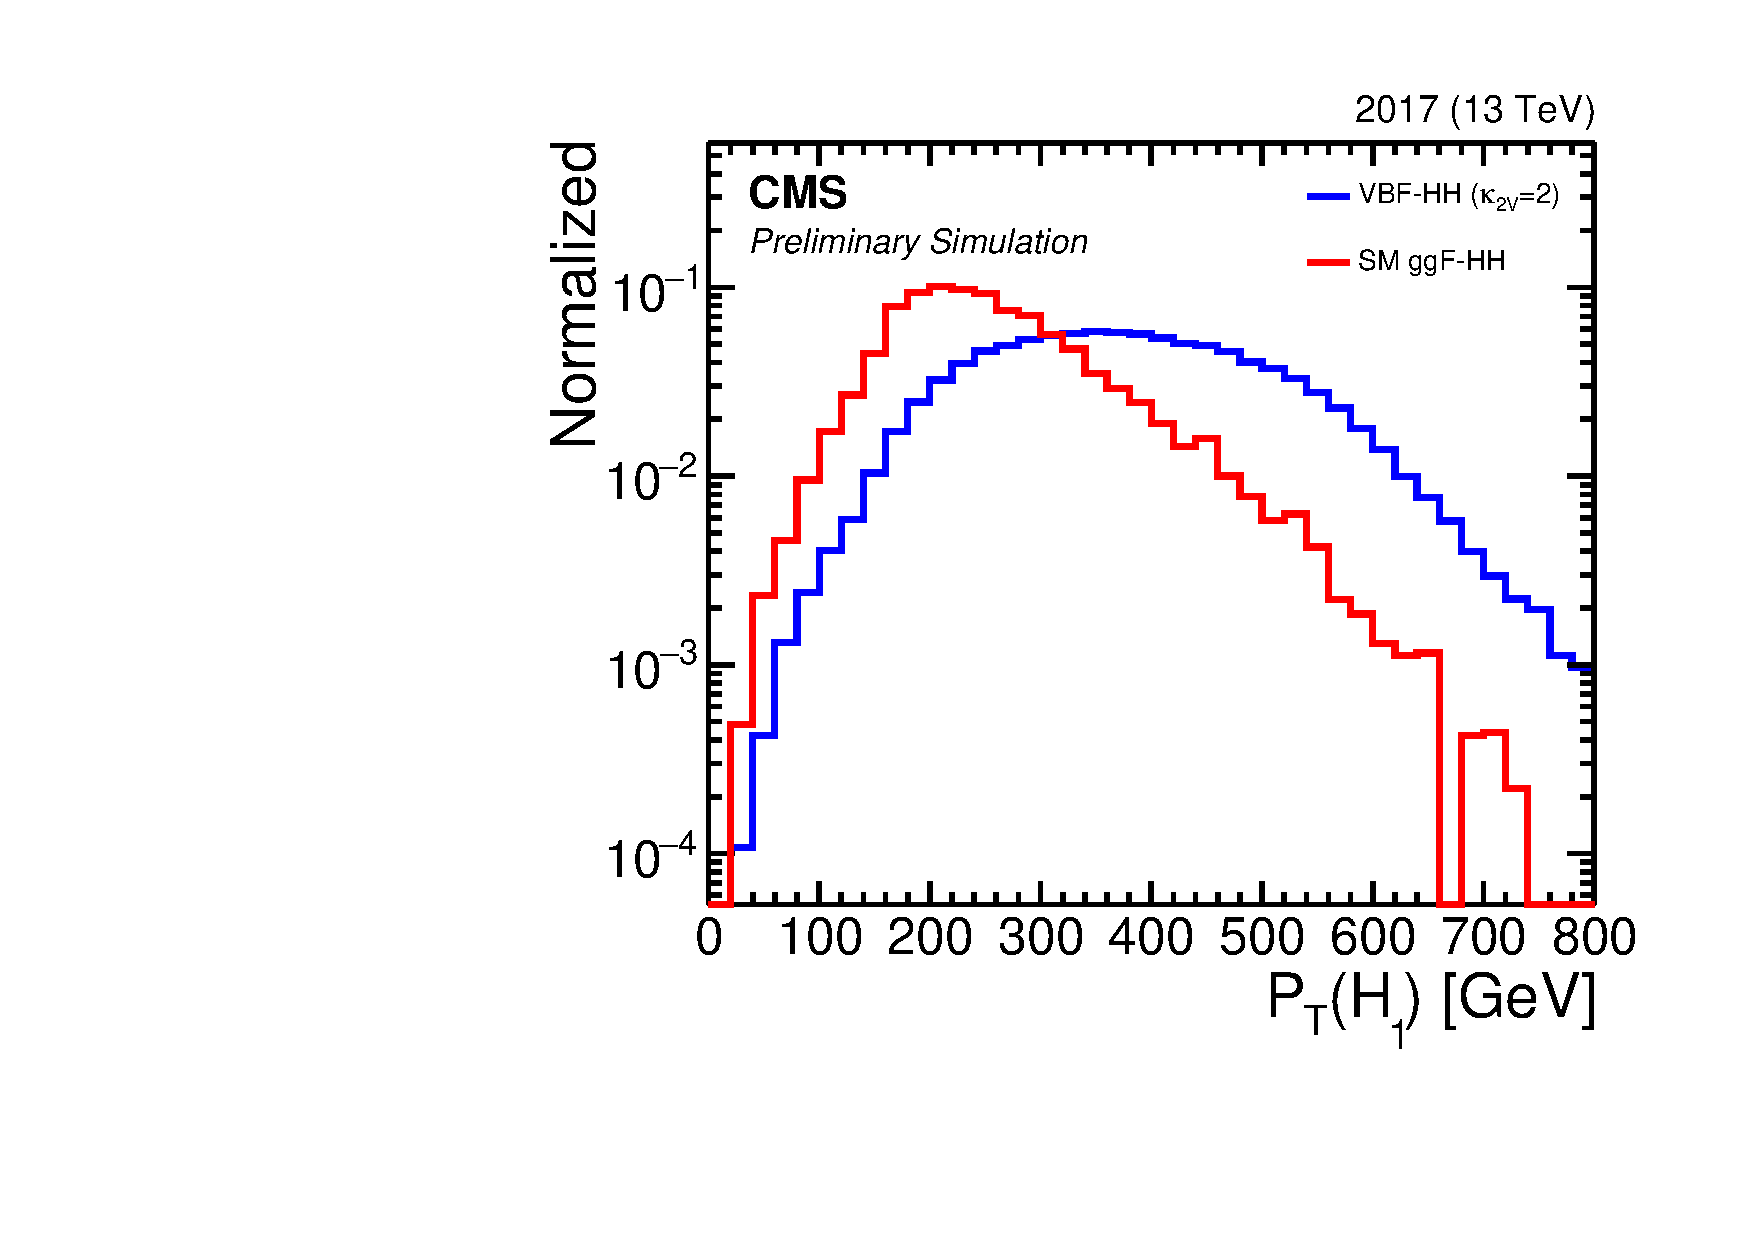
\includegraphics[width=0.27\linewidth]{Figures/AnalysisStrategy/eventselection/ggfkiller/2017ggfkiller/plot_2017_h_H1_pt.pdf}
\includegraphics[width=0.27\linewidth]{Figures/AnalysisStrategy/eventselection/ggfkiller/2017ggfkiller/plot_2017_h_H2_pt.pdf}
\includegraphics[width=0.27\linewidth]{Figures/AnalysisStrategy/eventselection/ggfkiller/2017ggfkiller/plot_2017_h_JJ_j1_pt.pdf} \\
\includegraphics[width=0.27\linewidth]{Figures/AnalysisStrategy/eventselection/ggfkiller/2017ggfkiller/plot_2017_h_JJ_j2_pt.pdf}
\includegraphics[width=0.27\linewidth]{Figures/AnalysisStrategy/eventselection/ggfkiller/2017ggfkiller/plot_2017_h_abs_costh_JJ_j1_vbfcm.pdf}
\includegraphics[width=0.27\linewidth]{Figures/AnalysisStrategy/eventselection/ggfkiller/2017ggfkiller/plot_2017_h_abs_costh_JJ_j2_vbfcm.pdf}
\includegraphics[width=0.27\linewidth]{Figures/AnalysisStrategy/eventselection/ggfkiller/2017ggfkiller/plot_2017_h_JJ_m.pdf}
\includegraphics[width=0.27\linewidth]{Figures/AnalysisStrategy/eventselection/ggfkiller/2017ggfkiller/plot_2017_h_H1H2_centrality.pdf}
\includegraphics[width=0.27\linewidth]{Figures/AnalysisStrategy/eventselection/ggfkiller/2017ggfkiller/plot_2017_h_JJ_eta.pdf}\\
\includegraphics[width=0.27\linewidth]{Figures/AnalysisStrategy/eventselection/ggfkiller/2017ggfkiller/plot_2017_h_h1h2_deltaR.pdf}
\includegraphics[width=0.27\linewidth]{Figures/AnalysisStrategy/eventselection/ggfkiller/2017ggfkiller/plot_2017_h_h1j1_deltaR.pdf}
\includegraphics[width=0.27\linewidth]{Figures/AnalysisStrategy/eventselection/ggfkiller/2017ggfkiller/plot_2017_h_h1j2_deltaR.pdf}\\
\includegraphics[width=0.27\linewidth]{Figures/AnalysisStrategy/eventselection/ggfkiller/2017ggfkiller/plot_2017_h_h2j1_deltaR.pdf}
\includegraphics[width=0.27\linewidth]{Figures/AnalysisStrategy/eventselection/ggfkiller/2017ggfkiller/plot_2017_h_h2j2_deltaR.pdf}
\end{center}
\caption[Distribution of the ggFKiller input  variables in 2017 simulation]{Distribution of the ggFKiller input  variables in 2017 simulation. The VBF with $\kvv=2$ (signal) is in solid blue, whereas SM ggF (background) is in solid red.}
\label{event_selection:fig:bdtvariables2017}
\end{figure}

\begin{figure}[htbp!]
\begin{center}
\includegraphics[width=0.27\linewidth]{Figures/AnalysisStrategy/eventselection/ggfkiller/2018ggfkiller/plot_2018_h_H1_pt.pdf}
\includegraphics[width=0.27\linewidth]{Figures/AnalysisStrategy/eventselection/ggfkiller/2018ggfkiller/plot_2018_h_H2_pt.pdf}
\includegraphics[width=0.27\linewidth]{Figures/AnalysisStrategy/eventselection/ggfkiller/2018ggfkiller/plot_2018_h_JJ_j1_pt.pdf} \\
\includegraphics[width=0.27\linewidth]{Figures/AnalysisStrategy/eventselection/ggfkiller/2018ggfkiller/plot_2018_h_JJ_j2_pt.pdf}
\includegraphics[width=0.27\linewidth]{Figures/AnalysisStrategy/eventselection/ggfkiller/2018ggfkiller/plot_2018_h_abs_costh_JJ_j1_vbfcm.pdf}
\includegraphics[width=0.27\linewidth]{Figures/AnalysisStrategy/eventselection/ggfkiller/2018ggfkiller/plot_2018_h_abs_costh_JJ_j2_vbfcm.pdf}
\includegraphics[width=0.27\linewidth]{Figures/AnalysisStrategy/eventselection/ggfkiller/2018ggfkiller/plot_2018_h_JJ_m.pdf}
\includegraphics[width=0.27\linewidth]{Figures/AnalysisStrategy/eventselection/ggfkiller/2017ggfkiller/plot_2017_h_H1H2_centrality.pdf}
\includegraphics[width=0.27\linewidth]{Figures/AnalysisStrategy/eventselection/ggfkiller/2018ggfkiller/plot_2018_h_JJ_eta.pdf}\\
\includegraphics[width=0.27\linewidth]{Figures/AnalysisStrategy/eventselection/ggfkiller/2018ggfkiller/plot_2018_h_h1h2_deltaR.pdf}
\includegraphics[width=0.27\linewidth]{Figures/AnalysisStrategy/eventselection/ggfkiller/2018ggfkiller/plot_2018_h_h1j1_deltaR.pdf}
\includegraphics[width=0.27\linewidth]{Figures/AnalysisStrategy/eventselection/ggfkiller/2018ggfkiller/plot_2018_h_h1j2_deltaR.pdf}\\
\includegraphics[width=0.27\linewidth]{Figures/AnalysisStrategy/eventselection/ggfkiller/2018ggfkiller/plot_2018_h_h2j1_deltaR.pdf}
\includegraphics[width=0.27\linewidth]{Figures/AnalysisStrategy/eventselection/ggfkiller/2018ggfkiller/plot_2018_h_h2j2_deltaR.pdf}
\end{center}
\caption[Distribution of the ggFKiller input  variables in 2018 simulation]{Distribution of the ggFKiller input  variables in 2018 simulation. The VBF with $\kvv=2$ (signal) is in solid blue, whereas SM ggF (background) is in solid red.}
\label{event_selection:fig:bdtvariables2018}
\end{figure}

\clearpage

\begin{figure}[htbp!]
\captionsetup[subfigure]{justification=centering}
\begin{center}
\subfloat[]{\includegraphics[width=0.42\linewidth]{Figures/AnalysisStrategy/eventselection/ggfkiller/2016ggfkiller/2016ggfkiller_importances.png}}
\subfloat[]{\includegraphics[width=0.42\linewidth]{Figures/AnalysisStrategy/eventselection/ggfkiller/2017ggfkiller/2017ggfkiller_importances.png}}\\
\subfloat[]{\includegraphics[width=0.42\linewidth]{Figures/AnalysisStrategy/eventselection/ggfkiller/2018ggfkiller/2018ggfkiller_importances.png}}
\end{center}
\caption[The relative importance of the ggFKiller training variables]{The relative importance of the ggFKiller training variables. Each row represents a particular simulation year: A) 2016, B) 2017, C) 2018.}
\label{event_selection:fig:ggfkillerimportance}
\end{figure}

The performance of the ggFKiller score in the train and test samples are presented depending on the year on Figure~\ref{event_selection:fig:ggfkillerper} A) B) and E), whereas the ROC curves in the test sample are presented depending on the year in Figure~\ref{event_selection:fig:ggfkillerper} B) D) and E). No signs of over-training are seen. The integral of the area under the curve (AUC) for the (train) test samples is (0.914) 0.908 in 2016, (0.923) 0.915 in 2017, and (0.923) 0.912 in 2018. For completeness, the relative variable importance is presented in Figure~\ref{event_selection:fig:ggfkillerimportance}.

\begin{figure}[htbp!]
\captionsetup[subfigure]{justification=centering}
\begin{center}
\subfloat[]{\includegraphics[width=0.45\linewidth]{Figures/AnalysisStrategy/eventselection/ggfkiller/2016ggfkiller/2016ggfkiller_ggfkiller_score_output.png}
\includegraphics[width=0.45\linewidth]{Figures/AnalysisStrategy/eventselection/ggfkiller/2016ggfkiller/2016ggfkiller_test_bdt_roc.png}}\\
\subfloat[]{\includegraphics[width=0.45\linewidth]{Figures/AnalysisStrategy/eventselection/ggfkiller/2017ggfkiller/2017ggfkiller_ggfkiller_score_output.png}
\includegraphics[width=0.45\linewidth]{Figures/AnalysisStrategy/eventselection/ggfkiller/2017ggfkiller/2017ggfkiller_test_bdt_roc.png}}\\
\subfloat[]{\includegraphics[width=0.45\linewidth]{Figures/AnalysisStrategy/eventselection/ggfkiller/2018ggfkiller/2018ggfkiller_ggfkiller_score_output.png}
\includegraphics[width=0.45\linewidth]{Figures/AnalysisStrategy/eventselection/ggfkiller/2018ggfkiller/2018ggfkiller_test_bdt_roc.png}}\\
\end{center}
\caption[Over-training check of the ggFKiller score]{Over-training check of the ggFKiller score. The left figure is the distribution of the score in train and test samples. The right figure is the test sample ROC curve performance. A) 2016, B) 2017 and C) 2018.}
\label{event_selection:fig:ggfkillerper}
\end{figure}

\chapter{Signal efficiencies vs Higgs boson couplings} \label{appendix:efficiencies}

\begin{figure}[htbp!]
\captionsetup[subfigure]{justification=centering}
\centering
\subfloat[]{\includegraphics[width=0.45\linewidth]{Figures/AnalysisStrategy/eventselection/efficiencies/eff_2016_vs_klambda.pdf}}
\subfloat[]{\includegraphics[width=0.45\linewidth]{Figures/AnalysisStrategy/eventselection/efficiencies/eff_2016_VBF_vs_kl.pdf}}\\
\subfloat[]{\includegraphics[width=0.45\linewidth]{Figures/AnalysisStrategy/eventselection/efficiencies/eff_2016_VBF_vs_C2V.pdf}}
\subfloat[]{\includegraphics[width=0.45\linewidth]{Figures/AnalysisStrategy/eventselection/efficiencies/eff_2016_VBF_vs_CV.pdf}}
\caption[Selection efficiency ($\epsilon$) of the 2016 selections versus the ggF and VBF couplings]{Selection efficiency ($\epsilon$) of the 2016 selections versus the ggF and VBF couplings. $\epsilon$ vs $\kl$ for the A) ggF and B) VBF signals, C) $\epsilon$ versus $\kvv$ and D) $\epsilon$ versus $\kv$ for the VBF signals. In all figures, the couplings that are not displayed on the x-axis are assumed to be fixed to the SM value. The crosses indicate the values obtained directly from the simulated samples, serving as cross-check to the values computed with the signal modeling procedure (denoted by the full circles).}
\label{fig:eff_sel_ggf_vbf_2016}
\end{figure}

\begin{figure}[htbp!]
\captionsetup[subfigure]{justification=centering}
\centering
\subfloat[]{\includegraphics[width=0.45\linewidth]{Figures/AnalysisStrategy/eventselection/efficiencies/eff_2017_vs_klambda.pdf}}
\subfloat[]{\includegraphics[width=0.45\linewidth]{Figures/AnalysisStrategy/eventselection/efficiencies/eff_2017_VBF_vs_kl.pdf}}\\
\subfloat[]{\includegraphics[width=0.45\linewidth]{Figures/AnalysisStrategy/eventselection/efficiencies/eff_2017_VBF_vs_C2V.pdf}}
\subfloat[]{\includegraphics[width=0.45\linewidth]{Figures/AnalysisStrategy/eventselection/efficiencies/eff_2017_VBF_vs_CV.pdf}} 
\caption[Selection efficiency ($\epsilon$) of the 2016 selections versus the ggF and VBF couplings]{Selection efficiency ($\epsilon$) of the 2017 selections versus the ggF and VBF couplings. $\epsilon$ vs $\kl$ for the A) ggF and B) VBF signals, C) $\epsilon$ versus $\kvv$ and D) $\epsilon$ versus $\kv$ for the VBF signals. In all figures, the couplings that are not displayed on the x-axis are assumed to be fixed to the SM value. The crosses indicate the values obtained directly from the simulated samples, serving as cross-check to the values computed with the signal modelling procedure (denoted by the full circles).}
\label{fig:eff_sel_ggf_vbf_2017}
\end{figure}

\chapter{List of simulation samples} \label{appendix:samples}

Simulated samples are used to model the signal processes as well as minor backgrounds.
A full list of the MC samples is reported in Tables~\ref{samples:tab:MC2016}, \ref{samples:tab:MC2017}, and \ref{samples:tab:MC2018} for the data taking conditions of 2016, 2017, and 2018, respectively. The normalization cross section also shown.% for the QCD samples are taken from~\cite{HbbMCSpreadsheet}.

\begin{table}[htb]
\centering
\caption[Summary of the MC samples used for the 2016 conditions]{\label{samples:tab:MC2016}Summary of the MC samples used for the 2016 conditions. All the samples are in the CMS NANOAODSIM data tier. The cross section includes the branching fraction.}
\begin{tabularx}{\textwidth}{lXr}
\hline
Process & Event generators & Cross section [pb]\\
\hline
QCD, $200  < H_\text{T} < 300~$GeV          & MadGraph, Pythia8  & 1710000 \\
QCD, $300  < H_\text{T} < 500~$GeV          & MadGraph, Pythia8  & 347500  \\
QCD, $500  < H_\text{T} < 700~$GeV          & MadGraph, Pythia8  & 32060   \\
QCD, $700  < H_\text{T} < 1000~$GeV         & MadGraph, Pythia8  & 6829    \\
QCD, $1000 < H_\text{T} < 1500~$GeV         & MadGraph, Pythia8  & 1207    \\
QCD, $1500 < H_\text{T} < 2000~$GeV         & MadGraph, Pythia8  & 120     \\
QCD, $H_\text{T} > 2000~$GeV                & MadGraph, Pythia8  & 25.25   \\
$\ttbar$                                    & PowHeg, Pythia8    & 831.76  \\
Single H$\to$bb  (ggF)                      & PowHeg, Pythia8    & 28.45   \\ 
Single H$\to$bb  (VBF)                      & PowHeg, Pythia8    & 2.202   \\ 
Single H$\to$bb  ($\mathrm{W^{+}H}$)        & PowHeg, Pythia8    & 0.3299  \\ 
Single H$\to$bb  ($\mathrm{W^{-}H}$)        & PowHeg, Pythia8    & 0.209   \\ 
Single H$\to$bb  ($\mathrm{ZH}$)            & PowHeg, Pythia8    & 0.359   \\ 
Single H$\to$bb  ($\ttbarh$)                & PowHeg, Pythia8    & 0.2953  \\ 
ZZ$\rightarrow$bbbb                         & MadGraph, Pythia8  & 0.3682  \\ 
gg$\to$HH$\to$bbbb (NLO),$\kl=1$            & PowHeg, Pythia8    & 0.010517\\
gg$\to$HH$\to$bbbb (NLO),$\kl=0$            & PowHeg, Pythia8    & 0.023618\\
gg$\to$HH$\to$bbbb (NLO),$\kl=2.45$         & PowHeg, Pythia8    & 0.004455\\
gg$\to$HH$\to$bbbb (NLO),$\kl=5$            & PowHeg, Pythia8    & 0.031072\\
VBF HH$\to$bbbb,$\kv=1$,  $\kvv=0$,$\kl=1$  & MadGraph, Pythia8  & 0.009169\\
VBF HH$\to$bbbb,$\kv=1$,  $\kvv=1$,$\kl=1$  & MadGraph, Pythia8  & 0.000585\\
VBF HH$\to$bbbb,$\kv=1$,  $\kvv=2$,$\kl=1$  & MadGraph, Pythia8  & 0.004823\\
VBF HH$\to$bbbb,$\kv=1$,  $\kvv=1$,$\kl=2$  & MadGraph, Pythia8  & 0.000482\\
VBF HH$\to$bbbb,$\kv=1$,  $\kvv=1$,$\kl=0$  & MadGraph, Pythia8  & 0.001558\\
VBF HH$\to$bbbb,$\kv=0.5$,$\kvv=1$,$\kl=1$  & MadGraph, Pythia8  & 0.003656\\
VBF HH$\to$bbbb,$\kv=1.5$,$\kvv=1$,$\kl=1$  & MadGraph, Pythia8  & 0.022412\\
EFT gg$\to$HH$\to$bbbb (LO)                 & MadGraph, Pythia8  & 0.010517\\
\hline
\end{tabularx}
\end{table}

\begin{table}[htb]
\centering
\caption[Summary of the MC samples used for the 2017 conditions]{\label{samples:tab:MC2017}Summary of the MC samples used for the 2017 conditions. The LO VBF HH samples $(**)$ were generated with Pythia8 dipole recoil mode on (default mode is off). All the samples are in the CMS NANOAODSIM data tier. The cross section includes the branching fraction.}
\begin{tabularx}{\textwidth}{lXr}
\hline
Process & Event generators & Cross section [pb]\\
\hline
QCD, $200  < H_\text{T} < 300$ GeV     & MadGraph, Pythia8   & 1547000 \\
QCD, $300  < H_\text{T} < 500$ GeV     & MadGraph, Pythia8   & 322600  \\
QCD, $500  < H_\text{T} < 700$ GeV     & MadGraph, Pythia8   & 29980   \\
QCD, $700  < H_\text{T} < 1000$ GeV    & MadGraph, Pythia8   & 6334    \\
QCD, $1000 < H_\text{T} < 1500$ GeV    & MadGraph, Pythia8   & 1088    \\
QCD, $1500 < H_\text{T} < 2000$ GeV    & MadGraph, Pythia8   & 99.11   \\
QCD, $H_\text{T} > 2000$ GeV           & MadGraph, Pythia8   & 20.23   \\
$\ttbar$ fully hadronic                & PowHeg, Pythia8     & 377.96  \\
$\ttbar$ semileptonic                  & PowHeg, Pythia8     & 365.34  \\
$\ttbar$ fully leptonic                & PowHeg, Pythia8     & 88.29   \\
Single H$\to$bb (ggF)                  & PowHeg, Pythia8     & 28.45   \\ 
Single H$\to$bb (VBF)                  & PowHeg, Pythia8     & 2.202   \\ 
Single H$\to$bb ($\mathrm{W^{+}H}$)    & PowHeg, Pythia8     & 0.3299  \\ 
Single H$\to$bb ($\mathrm{W^{-}H}$)    & PowHeg, Pythia8     & 0.209   \\ 
Single H$\to$bb ($\mathrm{ZH}$)        & PowHeg, Pythia8     & 0.359   \\ 
Single H$\to$bb ($\ttbar$H)            & PowHeg, Pythia8     & 0.2953  \\ 
ZZ$\rightarrow$4b                      & PowHeg, Pythia8     & 0.3682  \\ 
gg$\to$HH$\to$bbbb (NLO),$\kl = 1$     & PowHeg, Pythia8     & 0.010517\\
gg$\to$HH$\to$bbbb (NLO),$\kl = 0$     & PowHeg, Pythia8     & 0.023618\\
gg$\to$HH$\to$bbbb (NLO),$\kl = 2.45$  & PowHeg, Pythia8     & 0.004455\\
gg$\to$HH$\to$bbbb (NLO),$\kl = 5$     & PowHeg, Pythia8     & 0.031072\\
VBF HH$\to$bbbb,$\kv = 1$,  $\kvv = 1$,$\kl = 1$   &  MadGraph, Pythia8      & 0.009169\\
VBF HH$\to$bbbb,$\kv = 1$,  $\kvv = 1$,$\kl = 1$   &  MadGraph, Pythia8      & 0.000585\\
VBF HH$\to$bbbb,$\kv = 1$,  $\kvv = 2$,$\kl = 1$   &  MadGraph, Pythia8      & 0.004823\\
VBF HH$\to$bbbb,$\kv = 1$,  $\kvv = 1$,$\kl = 2$   &  MadGraph, Pythia8      & 0.000482\\
VBF HH$\to$bbbb,$\kv = 1$,  $\kvv = 1$,$\kl = 0$   &  MadGraph, Pythia8      & 0.001558\\
VBF HH$\to$bbbb,$\kv = 0.5$, $\kvv = 1$, $\kl = 1$ &  MadGraph, Pythia8      & 0.000585\\
VBF HH$\to$bbbb,$\kv = 1.5$, $\kvv = 1$, $\kl = 1$ &  MadGraph, Pythia8      & 0.004823\\
VBF HH$\to$bbbb, $(**)$,$\kv = 1$,  $\kvv = 1$,$\kl = 1$ & MadGraph, Pythia8 & 0.000585\\
VBF HH$\to$bbbb, $(**)$,$\kv = 1$,  $\kvv = 2$,$\kl = 1$ & MadGraph, Pythia8 & 0.004688\\
EFT gg$\to$HH$\to$bbbb                 & MadGraph, Pythia8   & 0.010517\\
\hline
\end{tabularx}
\end{table}


\begin{table}[htb]
\caption[Summary of the MC samples used for the 2018 conditions]{\label{samples:tab:MC2018}Summary of the MC samples used for the 2018 conditions. The LO VBF HH samples $(**)$ were generated with Pythia8 dipole recoil mode on (default mode is off). All the samples are in the NANOAODSIM data tier. The cross section includes the branching fraction.}
\begin{tabularx}{\textwidth}{lXr}
\hline
Process & Event generators & Cross section [pb]\\
\hline
QCD, $200  < H_\text{T} < 300~$GeV   & MadGraph, Pythia8   & 1547000  \\
QCD, $300  < H_\text{T} < 500~$GeV   & MadGraph, Pythia8   & 322600   \\
QCD, $500  < H_\text{T} < 700~$GeV   & MadGraph, Pythia8   & 29980    \\
QCD, $700  < H_\text{T} < 1000~$GeV  & MadGraph, Pythia8   & 6334     \\
QCD, $1000 < H_\text{T} < 1500~$GeV  & MadGraph, Pythia8   & 1088     \\
QCD, $1500 < H_\text{T} < 2000~$GeV  & MadGraph, Pythia8   & 99.11    \\
QCD, $H_\text{T} > 2000~$GeV         & MadGraph, Pythia8   & 20.23    \\
$\ttbar$ fully hadronic  & PowHeg, Pythia8                 & 377.96\\
$\ttbar$ semileptonic    & PowHeg, Pythia8                 & 365.34\\
$\ttbar$ fully leptonic  & PowHeg, Pythia8                 & 88.29\\
Single H$\to$bb  (ggF)                 & PowHeg, Pythia8      & 28.45 \\ 
Single H$\to$bb  (VBF)                 & PowHeg, Pythia8      & 2.202 \\
Single H$\to$bb  ($\mathrm{W^{+}H}$)   & PowHeg, Pythia8      & 0.3299\\ 
Single H$\to$bb  ($\mathrm{W^{-}H}$)   & PowHeg, Pythia8      & 0.209 \\ 
Single H$\to$bb  ($\mathrm{ZH}$)       & PowHeg, Pythia8      & 0.359 \\ 
Single H$\to$bb  ($\ttbarh$)           & PowHeg, Pythia8      & 0.2953\\ 
ZZ$\rightarrow$4b                   & PowHeg, Pythia8      & 0.3682\\ 
gg$\to$HH$\to$bbbb (NLO),$\kl=1$    & PowHeg, Pythia8      & 0.010517\\
gg$\to$HH$\to$bbbb (NLO),$\kl=0$    & PowHeg, Pythia8      & 0.023618\\
gg$\to$HH$\to$bbbb (NLO),$\kl=2.45$ & PowHeg, Pythia8      & 0.004455\\
gg$\to$HH$\to$bbbb (NLO),$\kl=5$    & PowHeg, Pythia8      & 0.031072\\
VBF HH$\to$bbbb,$\kv = 1$,  $\kvv = 0$,$\kl = 1$ &MadGraph, Pythia8          & 0.009169\\
VBF HH$\to$bbbb,$\kv = 1$,  $\kvv = 1$,$\kl = 1$ &MadGraph, Pythia8          & 0.000585\\
VBF HH$\to$bbbb,$\kv = 1$,  $\kvv = 2$,$\kl = 1$ &MadGraph, Pythia8          & 0.004823\\
VBF HH$\to$bbbb,$\kv = 1$,  $\kvv = 1$,$\kl = 2$ &MadGraph, Pythia8          & 0.000482\\
VBF HH$\to$bbbb,$\kv = 1$,  $\kvv = 1$,$\kl = 0$ &MadGraph, Pythia8          & 0.001558\\
VBF HH$\to$bbbb,$\kv = 0.5$,$\kvv = 1$,$\kl = 1$ &MadGraph, Pythia8          & 0.003656\\
VBF HH$\to$bbbb,$\kv = 1.5$,$\kvv = 1$,$\kl = 1$ &MadGraph, Pythia8          & 0.022412\\
VBF HH$\to$bbbb $(**)$,$\kv = 1$,  $\kvv = 1$,$\kl = 1$ &MadGraph, Pythia8   & 0.000585\\
VBF HH$\to$bbbb $(**)$,$\kv = 1$,  $\kvv = 2$,$\kl = 1$ &MadGraph, Pythia8   & 0.004823\\
EFT gg$\to$HH$\to$bbbb (LO)         & MadGraph, Pythia8    & 0.010517\\
\hline
\end{tabularx}
\end{table}

\chapter{Signal Model} \label{appendix:hhsignalmodel}
\section{Gluon Fusion Production} \label{sec:ggfsignalmodel}

Two different techniques are described to model the ggF HH signal. The first is the LO-reweighting model, which is the same used in all the 2016 nonresonant public results, including the bbbb analysis~\cite{bbbbcmsnr}, and the 2016 HH combination~\cite{cmshhrun1comb}. This event-based reweighting method has the advantage of using the full statistical power of the simulated samples, as it does attribute a positive weight to all simulated HH events. However, it is only applicable to LO signal samples because it cannot model events generated with the presence of parton emission at matrix element level and thus higher degrees of freedom (e.g. the NLO ggF signal simulated events). Consequently, another modeling is developed to model the signal using NLO samples.

{\bf{LO modeling:}} The ggF production at LO is a $2\to2$ scattering process. At the hard scattering level, the two Higgs bosons are produced back-to-back with the same transverse momentum. The azymuthal angle of the HH system is assumed to be isotropic. Furthermore, any parton distribution function effects in the simulation can be factored out as the Lorentz boost of the HH system is along the beam line. Consequently, the HH system is fully described by two variables: the invariant mass of the HH system ($\hhm$) and the absolute value of the cosine of the polar angle of one Higgs boson with respect to the beam axis in the HH rest frame ($|\cos\theta^{*}|$).

All available LO EFT HH simulated samples (SM and BSM) are combined and the resulting event distribution in the $\hhm$ and $|\cos\theta^{*}|$ variables is represented as a two-dimensional histogram with 55 bins and 4 bins and normalized to unity, respectively. A similar histogram is created for the SM sample only. The content of each histogram bin $k$ is denoted as $f^k_\text{comb}$ and $f^k_\text{SM}$, respectively. The event weight for an arbitrary coupling combination is defined as a function of $\hhm$ and $|\cos\theta^{*}|$ using the differential HH cross section ratio between the BSM target to the SM at each bin $k$.

From an EFT expansion assuming a generic HH production at LO, the ratio of the total cross section to the SM expectation ($\mathrm{R_{HH}}$) depends on the values of the five EFT anomalous couplings ($\kl$, $\kt$, $\cg$, $\cgg$, $\ctwo$). The ratio value for the bin $k$ ($\mathrm{R_{HH}^k}$) is a polynomial function of the couplings with coefficients $A_i^{k}$ (i=1,..,15), as seen in equation~\ref{eq:samples:HH-XS-BSMformula-LO}. From generated events, the value of $\mathrm{R_{HH}^k}$ is computed for different coupling combinations and interpolated as a function of them to get the associated $A_i^{j}$ coefficients. This procedure is further described in Ref.~\cite{Carvalho:2017vnu}. 
\begin{equation}
\label{eq:samples:HH-XS-BSMformula-LO}
\begin{split}
 \mathrm{R_{HH}^k} = \dfrac{\sigma_{HH}^k}{\sigma_{HH}^{k,\,\text{SM}}} & {\mathrel{\overset{\makebox[0pt]{\mbox{\normalfont\tiny\sffamily LO}}}{=}}}
 A_1^k \kt^4 +
 A_2^k \ctwo^2 +
 \left(A_3^k \kt^2 + A_4^k \cg^2 \right) \kl^2 + 
 A_5^k \cgg^2 + 
 \left(A_6^k \ctwo + A_7^k \kl\kt \right) \kt^2 \\ & + 
 \left(A_8^k \kt\kl + A_9^k \cg\kl \right) \ctwo  + 
 A_{10}^k \ctwo\cgg + 
 \left(A_{11}^k\cg\kl + A_{12}^k\cgg \right) \kt^2 \\ & + 
 \left(A_{13}^k\kl\cg + A_{14}^k\cgg \right) \kt\kl + 
 A_{15}^k \cg\cgg\kl
 \end{split}
\end{equation}

The event weight ($\omega$) used to model a generic BSM combination of Higgs boson couplings is fully determined from this parametrization and two-dimensional histograms. A value $\Omega$ is defined in equation~\ref{eq:samples:HHreweigthformula}, where it has been indicated explicitly the dependence on the five couplings of the ratio of the total ($R_{HH}$) and differential ($R_{HH}^j$) cross section to the SM prediction, completely determined from the $A_i^j$ coefficients. Then, the event weight $\omega$ is defined from $\Omega$ by normalizing it to the sum over all the $n$ simulated MC signal events considered (i.e. $\omega = \dfrac{\Omega}{\sum_n \Omega}$).  Therefore, the application of $\omega$ only modifies the differential event distribution but not the total normalization, and correctly accounts for changes in the acceptance after the selections.
\begin{equation}
\label{eq:samples:HHreweigthformula}
\begin{split}
\Omega(\kl, \kt, \ctwo, \cg, \cgg; k) & \equiv \dfrac{1}{f^k_\text{comb}} \cdot \dfrac{\sigma^k_{HH} (\kl, \kt, \ctwo, \cg, \cgg)}{\sigma_{HH} (\kl, \kt, \ctwo, \cg, \cgg)} \\
& = \dfrac{f^k_\text{SM}}{f^k_\text{comb}} \cdot \dfrac{R_{HH}^k (\kl, \kt, \ctwo, \cg, \cgg)}{R_{HH} (\kl, \kt, \ctwo, \cg, \cgg)}
\end{split}
\end{equation}

{\bf{NLO modeling:}}  The LO reweighting method cannot be applied for the case of NLO simulation, as the presence of an additional parton emitted at matrix level requires many more parameters to fully and correctly model the phase space. Consequently, a procedure based on the sum of different samples is used and restricted to the modeling of the $\kl$ and $\kt$ couplings only. 

The amplitude of the $\mathrm{gg\to HH}$ process can be generically expressed as $\mathcal{A} = \kl\kt T + \kt^2 B$. At the LO of the QCD expansion, $T$ and $B$ can be directly associated to the triangle and box diagrams of Fig.~\ref{fig:hhdiagrams} (a). This relation is also valid at any order of the QCD perturbative expansion because $T$ and $B$ will be the sum of all the diagrams with the same order in $\kl$ and $\kt$. Therefore, the ggF cross section can be expressed by the sum of three terms in equation~\ref{eq:samples:xsGGFHH}, where $\mathit{t} = |T|^2$, $\mathit{b} = |B|^2$, and $\mathit{i} = |T B^* + B^* T|$. The same relation is also valid for any differential cross section ($\mathrm{d\sigma/dx}$).
\begin{equation}
\label{eq:samples:xsGGFHH}
\sigma(\kl, \kt) \propto |\mathcal{A}|^2 = \kl^2\kt^2 \mathit{t} + \kt^4 \mathit{b} + \kl\kt^3 \mathit{i}
\end{equation}

Note that equation~\ref{eq:samples:xsGGFHH} can be written as equation~\ref{eq:samples:xsGGFHHmatrix}, where $\mathbf{c}(\kl, \kt)  = (\kl^2\kt^2, \, \kt^4, \, \kl\kt^3)$ is the vector of the coupling functions and $\mathbf{v} = (\mathit{t}, \, \mathit{b}, \, \mathit{i})$ is the vector of the values of the three terms. Therefore, for an arbitrary set of $(\kl, \kt)$ values, the HH signal can be described as the linear sum of three components. Moreover, the actual shape dependence is just on the ratio $\kl/\kt$, as $\mathbf{c}$ can be redefined as $\mathbf{c}(\kl, \kt) \rightarrow \kt^4 \, \mathbf{c}(\kl/\kt) = \kt^4 \, \left( (\kl/\kt)^2, 1, \kl/\kt \right)$. For simplicity, the $\kt = 1$ case is considered in the following derivation.
\begin{equation}
\label{eq:samples:xsGGFHHmatrix}
\sigma(\kl, \kt) = \mathbf{c}(\kl, \kt) \cdot \mathbf{v}
\end{equation}

The NLO MC POWHEG generator cannot individually generate events corresponding to the three terms. Furthermore, the direct sum of $\mathit{t}$, $\mathit{b}$, and $\mathit{i}$ is not optimal to model $\kl$ values around 2.5 because of the large cancellations due to the interference, which would require producing samples with large statistics. Equation~\eqref{eq:samples:xsGGFHH} also can be expressed in terms of a linear combination of three produced samples ($s_1$, $s_2$, $s_3$) with a specific choice of $\kl$. Applying equation~\eqref{eq:samples:xsGGFHH} to all the three samples, and denoting the 3 elements of the coupling vector for sample $s_k$ as $(c_k^1, \, c_k^2, \, c_k^3)$, the one obtains the equation~\ref{eq:samples:bigGGFmatrix}. The three $\sigma_i$ values are known from the POWHEG generator. 
\begin{equation}
\label{eq:samples:bigGGFmatrix}
\begin{pmatrix} \sigma_1 \\ \sigma_2 \\ \sigma_3 \end{pmatrix} = 
\begin{pmatrix}
c_1^1  & c_1^2 & c_1^3 \\
c_2^1  & c_2^2 & c_2^3 \\
c_3^1  & c_3^2 & c_3^3
\end{pmatrix}
\begin{pmatrix} \mathit{t} \\ \mathit{b} \\ \mathit{i} \end{pmatrix}
\end{equation}
A simplified form of equation~\ref{eq:samples:bigGGFmatrix} is  $\boldsymbol{\sigma} = \mathbf{C} \mathbf{v}$. Then, inverting the matrix $\mathbf{C}$, one obtains the relation $\mathbf{v} = \mathbf{C}^{-1} \boldsymbol{\sigma}$. By substituting it in equation~\eqref{eq:samples:xsGGFHHmatrix}, one gets the parametrization defined in equation~\ref{eq:functionsggfmodel}. This relation also holds for differential $\mathrm{d\sigma/dx}$ distributions. 
\begin{equation}
\label{eq:functionsggfmodel}
\sigma(\kl) = \mathbf{c}^{T}(\kl) \mathbf{C}^{-1} \boldsymbol{\sigma}
\end{equation}
Using this method, a generic value of $\kl$ can be modeled as the sum of three NLO generated samples, scaling each sample $s_i$ by functions of $\kl$ that are derived by equation~\ref{eq:functionsggfmodel}. The choice of the three $\kl$ values can be optimized based on the statistical precision, as some multiplicative coefficients may be negative depending on the coupling choice. For selecting the optimal coupling choice, redundancy and cross-check of the method, four samples were generated ($\kl = 0, 1, 2.45, 5$). The optimal coupling choice is $\kl = 1, 2.45, 5$.

\section{Vector Boson Fusion Production} \label{sec:vbfsignalmodel}
A VBF event-based reweighting method is not feasible due to the high number of parameters needed to describe the HHjj system. Then, the modeling of the VBF signals follows the same idea as the ggF NLO component sum method presented above. In analogy to equation~\ref{eq:samples:xsGGFHH}, the cross section can be described as equation~\ref{eq:samples:xsVBFHHmatrix} based on the Figure~\ref{fig:hhdiagrams} (b) diagrams, where $a$, $b$ and $c$ are the amplitude squared terms and $i_{ab}$, $i_{ac}$, and $i_{bc}$ are the interference terms. 
\begin{equation}
\label{eq:samples:xsVBFHHmatrix}
\sigma(\kl, \kv, \kvv) = 
\begin{pmatrix}
\kv^2\kl^2 \\
\kv^4 \\
\kvv^2 \\
\kv^3\kl \\
\kv\kl\kvv \\
\kv^2\kvv
\end{pmatrix}
\cdot
\begin{pmatrix}
a \\ b \\ c \\ i_{ab} \\ i_{ac} \\ i_{bc}
\end{pmatrix}
\end{equation}

In the VBF component sum model, six samples $s_i$ are generated. Each sample has a cross section $\sigma_i$ taken from the MadGraph LO generator. Following the same formal procedure as with the ggF model, the final modeling of the VBF cross section parametrization is derived as equation~\ref{eq:functionsvbfmodel}, where $\mathbf{C}^{-1}$ is a $6\times6$ matrix. To optimize this model based on the statistical precision and validation, seven samples were generated with the following $(\kl,\kv, \kvv)$ couplings: (1,1,1), (1,1,0), (1,1,2), (2,1,1), (0,1,1), (1,0.5,1) and (1.1.5,1). The best choice of six samples drops the sample $(\kl,\kv, \kvv)~=~(1.0.5,1)$. 
\begin{equation}
\label{eq:functionsvbfmodel}
\sigma(\kl, \kv, \kvv) = \mathbf{c}^{T}(\kl, \kv, \kvv) \mathbf{C}^{-1} \boldsymbol{\sigma}
\end{equation}

\chapter{Background modeling} \label{appendix:bkgmodel}

\section{BDT Reweighting Hyperparameters}

\begin{table}[htbp!]
\centering
\caption[Best BDT-reweigher hyperparameters in 2016 analysis control region]{\label{bkg:tab:bdtregparameters2016}Best BDT-reweigher hyperparameters in 2016 analysis control region.}
\begin{tabularx}{\textwidth}{lXXX}
    \hline 
    Hyperparameters           & ggF Cat. 1     & ggF Cat. 2    &  VBF  Cat. 1 \\
    \hline
    \small Number of trees    & \small  50   & \small 50   & \small  125  \\
    \small Max. depth         & \small  2    & \small  2   & \small  3    \\
    \small Learning rate      & \small 0.5   & \small 0.5  & \small  0.1  \\
    \small Min. samples leaf  & \small  5    & \small 20   & \small  20   \\
    \small Subsample          & \small 0.6   & \small 0.6  & \small 0.6   \\
    \hline
\end{tabularx}
\end{table}

\begin{table}[htbp!]
\centering
\caption[Best BDT-reweigher hyperparameters in 2017-2018 analysis control region]{\label{bkg:tab:bdtregparameters20172018}Best BDT-reweigher hyperparameters in 2017-2018 analysis control region.}
\begin{tabularx}{\textwidth}{lXXX}
    \hline 
    Hyperparameters           & ggF Cat. 1     & ggF Cat. 2    &  VBF  Cat. 1 \\
    \hline
    \small Number of trees    & \small  50   & \small 150   & \small  50   \\
    \small Max. depth         & \small  2    & \small  3   & \small  2    \\
    \small Learning rate      & \small 0.5   & \small  0.1 & \small  0.5  \\
    \small Min. samples leaf  & \small 10   & \small 5  & \small 20   \\
    \small Subsample          & \small 0.6   & \small 0.6  & \small 0.6   \\
    \hline
\end{tabularx}
\end{table}

\begin{table}[htbp!]
\centering
\caption[Best BDT-reweigher hyperparameters in 2016 validation test]{\label{bkg:tab:bdtregparametersval2016}Best BDT-reweigher hyperparameters in 2016 validation test.}
\begin{tabularx}{\textwidth}{lXXX}
    \hline 
    Hyperparameters           & ggF Cat. 1     & ggF Cat. 2    &  VBF Cat. 1 \\
    \hline
    \small Number of trees    & \small  150  & \small 75   & \small  50   \\
    \small Max. depth         & \small  4    & \small  3   & \small  2    \\
    \small Learning rate      & \small 0.1   & \small 0.5  & \small  0.05  \\
    \small Min. samples leaf  & \small 10    & \small 5    & \small 5   \\
    \small Subsample          & \small 0.6   & \small 0.6  & \small 0.6   \\
   \hline
\end{tabularx}
\end{table}

\begin{table}[htbp!]
\centering
\caption[Best BDT-reweigher hyperparameters in 2017-2018 validation test]{\label{bkg:tab:bdtregparametersval20172018}Best BDT-reweigher hyperparameters in 2017-2018 validation test.}
\begin{tabularx}{\textwidth}{lXXX}
    \hline 
    Hyperparameters           & ggF Cat. 1     & ggF Cat. 2    &  VBF  Cat. 1 \\
    \hline
    \small Number of trees    & \small  75   & \small 125  & \small  125   \\
    \small Max. depth         & \small  2    & \small  3   & \small  2    \\
    \small Learning rate      & \small 0.5   & \small  0.1 & \small  0.1  \\
    \small Min. samples leaf  & \small  10   & \small 1    & \small 10   \\
    \small Subsample          & \small 0.6   & \small 0.6  & \small 0.6   \\
    \hline
\end{tabularx}
\end{table}


\clearpage

\section{Analysis Control Region Results}

This section presents the data and background model distributions with the BDT-reweighting applied in the analysis control region. Figures~\ref{bkg:fig:bdtregvarggf1_2016}, \ref{bkg:fig:bdtregvarggf2_2016} and \ref{bkg:fig:bdtregvarvbf1_2016} show the results in 2016 ggF category 1, 2016 ggF category 2, and 2016 VBF category 1, respectively. Figures~\ref{bkg:fig:bdtregvarggf1_20172018}, \ref{bkg:fig:bdtregvarggf2_20172018} and \ref{bkg:fig:bdtregvarvbf1_20172018} show the results in 2016 ggF category 1, 2016 ggF category 2, and 2016 VBF category 1, respectively.

\begin{figure}[htbp!]
\begin{center}
\includegraphics[width=0.24\linewidth]{Figures/Modeling/background/plotsDatadrivenWithBDT/2016/GGFcateg1_CR_110/Histogram/plot2016_H1_b1_ptRegressed_Btag4_GGFcateg1_CR_110_Histogram_log.pdf}
\includegraphics[width=0.24\linewidth]{Figures/Modeling/background/plotsDatadrivenWithBDT/2016/GGFcateg1_CR_110/Histogram/plot2016_H2_b1_ptRegressed_Btag4_GGFcateg1_CR_110_Histogram_log.pdf}
\includegraphics[width=0.24\linewidth]{Figures/Modeling/background/plotsDatadrivenWithBDT/2016/GGFcateg1_CR_110/Histogram/plot2016_H1_b2_ptRegressed_Btag4_GGFcateg1_CR_110_Histogram_log.pdf}
\includegraphics[width=0.24\linewidth]{Figures/Modeling/background/plotsDatadrivenWithBDT/2016/GGFcateg1_CR_110/Histogram/plot2016_H2_b2_ptRegressed_Btag4_GGFcateg1_CR_110_Histogram_log.pdf}\\
\includegraphics[width=0.24\linewidth]{Figures/Modeling/background/plotsDatadrivenWithBDT/2016/GGFcateg1_CR_110/Histogram/plot2016_H1_m_Btag4_GGFcateg1_CR_110_Histogram_log.pdf}
\includegraphics[width=0.24\linewidth]{Figures/Modeling/background/plotsDatadrivenWithBDT/2016/GGFcateg1_CR_110/Histogram/plot2016_H2_m_Btag4_GGFcateg1_CR_110_Histogram_log.pdf}
\includegraphics[width=0.24\linewidth]{Figures/Modeling/background/plotsDatadrivenWithBDT/2016/GGFcateg1_CR_110/Histogram/plot2016_H1_pt_Btag4_GGFcateg1_CR_110_Histogram_log.pdf}
\includegraphics[width=0.24\linewidth]{Figures/Modeling/background/plotsDatadrivenWithBDT/2016/GGFcateg1_CR_110/Histogram/plot2016_H2_pt_Btag4_GGFcateg1_CR_110_Histogram_log.pdf}\\
\includegraphics[width=0.24\linewidth]{Figures/Modeling/background/plotsDatadrivenWithBDT/2016/GGFcateg1_CR_110/Histogram/plot2016_HH_m_Btag4_GGFcateg1_CR_110_Histogram_log.pdf}
\includegraphics[width=0.24\linewidth]{Figures/Modeling/background/plotsDatadrivenWithBDT/2016/GGFcateg1_CR_110/Histogram/plot2016_H1_bb_deltaR_Btag4_GGFcateg1_CR_110_Histogram_log.pdf}
\includegraphics[width=0.24\linewidth]{Figures/Modeling/background/plotsDatadrivenWithBDT/2016/GGFcateg1_CR_110/Histogram/plot2016_H2_bb_deltaR_Btag4_GGFcateg1_CR_110_Histogram_log.pdf}
\includegraphics[width=0.24\linewidth]{Figures/Modeling/background/plotsDatadrivenWithBDT/2016/GGFcateg1_CR_110/Histogram/plot2016_h1h2_deltaEta_Btag4_GGFcateg1_CR_110_Histogram_log.pdf}\\
\includegraphics[width=0.24\linewidth]{Figures/Modeling/background/plotsDatadrivenWithBDT/2016/GGFcateg1_CR_110/Histogram/plot2016_abs_costh_H1_ggfcm_Btag4_GGFcateg1_CR_110_Histogram_log.pdf}
\includegraphics[width=0.24\linewidth]{Figures/Modeling/background/plotsDatadrivenWithBDT/2016/GGFcateg1_CR_110/Histogram/plot2016_sum_3b_bres_Btag4_GGFcateg1_CR_110_Histogram_log.pdf}
\includegraphics[width=0.24\linewidth]{Figures/Modeling/background/plotsDatadrivenWithBDT/2016/GGFcateg1_CR_110/Histogram/plot2016_HH_pt_Btag4_GGFcateg1_CR_110_Histogram_log.pdf}
\includegraphics[width=0.24\linewidth]{Figures/Modeling/background/plotsDatadrivenWithBDT/2016/GGFcateg1_CR_110/Histogram/plot2016_sum_4b_pt_Btag4_GGFcateg1_CR_110_Histogram_log.pdf}\\
\includegraphics[width=0.24\linewidth]{Figures/Modeling/background/plotsDatadrivenWithBDT/2016/GGFcateg1_CR_110/Histogram/plot2016_abs_costh_H1_b1_h1cm_Btag4_GGFcateg1_CR_110_Histogram_log.pdf}
\includegraphics[width=0.24\linewidth]{Figures/Modeling/background/plotsDatadrivenWithBDT/2016/GGFcateg1_CR_110/Histogram/plot2016_nBtagTightonMediumWP_Btag4_GGFcateg1_CR_110_Histogram_log.pdf}
\includegraphics[width=0.24\linewidth]{Figures/Modeling/background/plotsDatadrivenWithBDT/2016/GGFcateg1_CR_110/Histogram/plot2016_min_4b_deltaR_Btag4_GGFcateg1_CR_110_Histogram_log.pdf}
\includegraphics[width=0.24\linewidth]{Figures/Modeling/background/plotsDatadrivenWithBDT/2016/GGFcateg1_CR_110/Histogram/plot2016_max_4b_deltaEta_Btag4_GGFcateg1_CR_110_Histogram_log.pdf}
\end{center}
\caption{Data versus background modeling agreement of the variables of the BDT-reweighter training (with  BDT-reweighting) in 2016 ggF category 1.}
\label{bkg:fig:bdtregvarggf1_2016}
\end{figure}

\begin{figure}[htbp!]
\begin{center}
\includegraphics[width=0.24\linewidth]{Figures/Modeling/background/plotsDatadrivenWithBDT/2016/GGFcateg2_CR_110/Histogram/plot2016_H1_b1_ptRegressed_Btag4_GGFcateg2_CR_110_Histogram_log.pdf}
\includegraphics[width=0.24\linewidth]{Figures/Modeling/background/plotsDatadrivenWithBDT/2016/GGFcateg2_CR_110/Histogram/plot2016_H2_b1_ptRegressed_Btag4_GGFcateg2_CR_110_Histogram_log.pdf}
\includegraphics[width=0.24\linewidth]{Figures/Modeling/background/plotsDatadrivenWithBDT/2016/GGFcateg2_CR_110/Histogram/plot2016_H1_b2_ptRegressed_Btag4_GGFcateg2_CR_110_Histogram_log.pdf}
\includegraphics[width=0.24\linewidth]{Figures/Modeling/background/plotsDatadrivenWithBDT/2016/GGFcateg2_CR_110/Histogram/plot2016_H2_b2_ptRegressed_Btag4_GGFcateg2_CR_110_Histogram_log.pdf}\\
\includegraphics[width=0.24\linewidth]{Figures/Modeling/background/plotsDatadrivenWithBDT/2016/GGFcateg2_CR_110/Histogram/plot2016_H1_m_Btag4_GGFcateg2_CR_110_Histogram_log.pdf}
\includegraphics[width=0.24\linewidth]{Figures/Modeling/background/plotsDatadrivenWithBDT/2016/GGFcateg2_CR_110/Histogram/plot2016_H2_m_Btag4_GGFcateg2_CR_110_Histogram_log.pdf}
\includegraphics[width=0.24\linewidth]{Figures/Modeling/background/plotsDatadrivenWithBDT/2016/GGFcateg2_CR_110/Histogram/plot2016_H1_pt_Btag4_GGFcateg2_CR_110_Histogram_log.pdf}
\includegraphics[width=0.24\linewidth]{Figures/Modeling/background/plotsDatadrivenWithBDT/2016/GGFcateg2_CR_110/Histogram/plot2016_H2_pt_Btag4_GGFcateg2_CR_110_Histogram_log.pdf}\\
\includegraphics[width=0.24\linewidth]{Figures/Modeling/background/plotsDatadrivenWithBDT/2016/GGFcateg2_CR_110/Histogram/plot2016_HH_m_Btag4_GGFcateg2_CR_110_Histogram_log.pdf}
\includegraphics[width=0.24\linewidth]{Figures/Modeling/background/plotsDatadrivenWithBDT/2016/GGFcateg2_CR_110/Histogram/plot2016_H1_bb_deltaR_Btag4_GGFcateg2_CR_110_Histogram_log.pdf}
\includegraphics[width=0.24\linewidth]{Figures/Modeling/background/plotsDatadrivenWithBDT/2016/GGFcateg2_CR_110/Histogram/plot2016_H2_bb_deltaR_Btag4_GGFcateg2_CR_110_Histogram_log.pdf}
\includegraphics[width=0.24\linewidth]{Figures/Modeling/background/plotsDatadrivenWithBDT/2016/GGFcateg2_CR_110/Histogram/plot2016_h1h2_deltaEta_Btag4_GGFcateg2_CR_110_Histogram_log.pdf}\\
\includegraphics[width=0.24\linewidth]{Figures/Modeling/background/plotsDatadrivenWithBDT/2016/GGFcateg2_CR_110/Histogram/plot2016_abs_costh_H1_ggfcm_Btag4_GGFcateg2_CR_110_Histogram_log.pdf}
\includegraphics[width=0.24\linewidth]{Figures/Modeling/background/plotsDatadrivenWithBDT/2016/GGFcateg2_CR_110/Histogram/plot2016_sum_3b_bres_Btag4_GGFcateg2_CR_110_Histogram_log.pdf}
\includegraphics[width=0.24\linewidth]{Figures/Modeling/background/plotsDatadrivenWithBDT/2016/GGFcateg2_CR_110/Histogram/plot2016_HH_pt_Btag4_GGFcateg2_CR_110_Histogram_log.pdf}
\includegraphics[width=0.24\linewidth]{Figures/Modeling/background/plotsDatadrivenWithBDT/2016/GGFcateg2_CR_110/Histogram/plot2016_sum_4b_pt_Btag4_GGFcateg2_CR_110_Histogram_log.pdf}\\
\includegraphics[width=0.24\linewidth]{Figures/Modeling/background/plotsDatadrivenWithBDT/2016/GGFcateg2_CR_110/Histogram/plot2016_abs_costh_H1_b1_h1cm_Btag4_GGFcateg2_CR_110_Histogram_log.pdf}
\includegraphics[width=0.24\linewidth]{Figures/Modeling/background/plotsDatadrivenWithBDT/2016/GGFcateg2_CR_110/Histogram/plot2016_nBtagTightonMediumWP_Btag4_GGFcateg2_CR_110_Histogram_log.pdf}
\includegraphics[width=0.24\linewidth]{Figures/Modeling/background/plotsDatadrivenWithBDT/2016/GGFcateg2_CR_110/Histogram/plot2016_min_4b_deltaR_Btag4_GGFcateg2_CR_110_Histogram_log.pdf}
\includegraphics[width=0.24\linewidth]{Figures/Modeling/background/plotsDatadrivenWithBDT/2016/GGFcateg2_CR_110/Histogram/plot2016_max_4b_deltaEta_Btag4_GGFcateg2_CR_110_Histogram_log.pdf}
\end{center}
\caption{Data versus background modeling agreement of the variables of the BDT-reweighter training (with  BDT-reweighting) in 2016 ggF category 2.}
\label{bkg:fig:bdtregvarggf2_2016}
\end{figure}

\begin{figure}[htbp!]
\begin{center}
\includegraphics[width=0.24\linewidth]{Figures/Modeling/background/plotsDatadrivenWithBDT/20172018/GGFcateg1_CR_110/Histogram/plot20172018_H1_b1_ptRegressed_Btag4_GGFcateg1_CR_110_Histogram_log.pdf}
\includegraphics[width=0.24\linewidth]{Figures/Modeling/background/plotsDatadrivenWithBDT/20172018/GGFcateg1_CR_110/Histogram/plot20172018_H2_b1_ptRegressed_Btag4_GGFcateg1_CR_110_Histogram_log.pdf}
\includegraphics[width=0.24\linewidth]{Figures/Modeling/background/plotsDatadrivenWithBDT/20172018/GGFcateg1_CR_110/Histogram/plot20172018_H1_b2_ptRegressed_Btag4_GGFcateg1_CR_110_Histogram_log.pdf}
\includegraphics[width=0.24\linewidth]{Figures/Modeling/background/plotsDatadrivenWithBDT/20172018/GGFcateg1_CR_110/Histogram/plot20172018_H2_b2_ptRegressed_Btag4_GGFcateg1_CR_110_Histogram_log.pdf}\\
\includegraphics[width=0.24\linewidth]{Figures/Modeling/background/plotsDatadrivenWithBDT/20172018/GGFcateg1_CR_110/Histogram/plot20172018_H1_m_Btag4_GGFcateg1_CR_110_Histogram_log.pdf}
\includegraphics[width=0.24\linewidth]{Figures/Modeling/background/plotsDatadrivenWithBDT/20172018/GGFcateg1_CR_110/Histogram/plot20172018_H2_m_Btag4_GGFcateg1_CR_110_Histogram_log.pdf}
\includegraphics[width=0.24\linewidth]{Figures/Modeling/background/plotsDatadrivenWithBDT/20172018/GGFcateg1_CR_110/Histogram/plot20172018_H1_pt_Btag4_GGFcateg1_CR_110_Histogram_log.pdf}
\includegraphics[width=0.24\linewidth]{Figures/Modeling/background/plotsDatadrivenWithBDT/20172018/GGFcateg1_CR_110/Histogram/plot20172018_H2_pt_Btag4_GGFcateg1_CR_110_Histogram_log.pdf}\\
\includegraphics[width=0.24\linewidth]{Figures/Modeling/background/plotsDatadrivenWithBDT/20172018/GGFcateg1_CR_110/Histogram/plot20172018_HH_m_Btag4_GGFcateg1_CR_110_Histogram_log.pdf}
\includegraphics[width=0.24\linewidth]{Figures/Modeling/background/plotsDatadrivenWithBDT/20172018/GGFcateg1_CR_110/Histogram/plot20172018_H1_bb_deltaR_Btag4_GGFcateg1_CR_110_Histogram_log.pdf}
\includegraphics[width=0.24\linewidth]{Figures/Modeling/background/plotsDatadrivenWithBDT/20172018/GGFcateg1_CR_110/Histogram/plot20172018_H2_bb_deltaR_Btag4_GGFcateg1_CR_110_Histogram_log.pdf}
\includegraphics[width=0.24\linewidth]{Figures/Modeling/background/plotsDatadrivenWithBDT/20172018/GGFcateg1_CR_110/Histogram/plot20172018_h1h2_deltaEta_Btag4_GGFcateg1_CR_110_Histogram_log.pdf}\\
\includegraphics[width=0.24\linewidth]{Figures/Modeling/background/plotsDatadrivenWithBDT/20172018/GGFcateg1_CR_110/Histogram/plot20172018_abs_costh_H1_ggfcm_Btag4_GGFcateg1_CR_110_Histogram_log.pdf}
\includegraphics[width=0.24\linewidth]{Figures/Modeling/background/plotsDatadrivenWithBDT/20172018/GGFcateg1_CR_110/Histogram/plot20172018_sum_3b_bres_Btag4_GGFcateg1_CR_110_Histogram_log.pdf}
\includegraphics[width=0.24\linewidth]{Figures/Modeling/background/plotsDatadrivenWithBDT/20172018/GGFcateg1_CR_110/Histogram/plot20172018_HH_pt_Btag4_GGFcateg1_CR_110_Histogram_log.pdf}
\includegraphics[width=0.24\linewidth]{Figures/Modeling/background/plotsDatadrivenWithBDT/20172018/GGFcateg1_CR_110/Histogram/plot20172018_sum_4b_pt_Btag4_GGFcateg1_CR_110_Histogram_log.pdf}\\
\includegraphics[width=0.24\linewidth]{Figures/Modeling/background/plotsDatadrivenWithBDT/20172018/GGFcateg1_CR_110/Histogram/plot20172018_abs_costh_H1_b1_h1cm_Btag4_GGFcateg1_CR_110_Histogram_log.pdf}
\includegraphics[width=0.24\linewidth]{Figures/Modeling/background/plotsDatadrivenWithBDT/20172018/GGFcateg1_CR_110/Histogram/plot20172018_nBtagTightonMediumWP_Btag4_GGFcateg1_CR_110_Histogram_log.pdf}
\includegraphics[width=0.24\linewidth]{Figures/Modeling/background/plotsDatadrivenWithBDT/20172018/GGFcateg1_CR_110/Histogram/plot20172018_min_4b_deltaR_Btag4_GGFcateg1_CR_110_Histogram_log.pdf}
\includegraphics[width=0.24\linewidth]{Figures/Modeling/background/plotsDatadrivenWithBDT/20172018/GGFcateg1_CR_110/Histogram/plot20172018_max_4b_deltaEta_Btag4_GGFcateg1_CR_110_Histogram_log.pdf}
\end{center}
\caption{Data versus background modeling agreement of the variables of the BDT-reweighter training (with BDT-reweighting) in 20172018 ggF category 1.}
\label{bkg:fig:bdtregvarggf1_20172018}
\end{figure}

\begin{figure}[htbp!]
\begin{center}
\includegraphics[width=0.24\linewidth]{Figures/Modeling/background/plotsDatadrivenWithBDT/20172018/GGFcateg2_CR_110/Histogram/plot20172018_H1_b1_ptRegressed_Btag4_GGFcateg2_CR_110_Histogram_log.pdf}
\includegraphics[width=0.24\linewidth]{Figures/Modeling/background/plotsDatadrivenWithBDT/20172018/GGFcateg2_CR_110/Histogram/plot20172018_H2_b1_ptRegressed_Btag4_GGFcateg2_CR_110_Histogram_log.pdf}
\includegraphics[width=0.24\linewidth]{Figures/Modeling/background/plotsDatadrivenWithBDT/20172018/GGFcateg2_CR_110/Histogram/plot20172018_H1_b2_ptRegressed_Btag4_GGFcateg2_CR_110_Histogram_log.pdf}
\includegraphics[width=0.24\linewidth]{Figures/Modeling/background/plotsDatadrivenWithBDT/20172018/GGFcateg2_CR_110/Histogram/plot20172018_H2_b2_ptRegressed_Btag4_GGFcateg2_CR_110_Histogram_log.pdf}\\
\includegraphics[width=0.24\linewidth]{Figures/Modeling/background/plotsDatadrivenWithBDT/20172018/GGFcateg2_CR_110/Histogram/plot20172018_H1_m_Btag4_GGFcateg2_CR_110_Histogram_log.pdf}
\includegraphics[width=0.24\linewidth]{Figures/Modeling/background/plotsDatadrivenWithBDT/20172018/GGFcateg2_CR_110/Histogram/plot20172018_H2_m_Btag4_GGFcateg2_CR_110_Histogram_log.pdf}
\includegraphics[width=0.24\linewidth]{Figures/Modeling/background/plotsDatadrivenWithBDT/20172018/GGFcateg2_CR_110/Histogram/plot20172018_H1_pt_Btag4_GGFcateg2_CR_110_Histogram_log.pdf}
\includegraphics[width=0.24\linewidth]{Figures/Modeling/background/plotsDatadrivenWithBDT/20172018/GGFcateg2_CR_110/Histogram/plot20172018_H2_pt_Btag4_GGFcateg2_CR_110_Histogram_log.pdf}\\
\includegraphics[width=0.24\linewidth]{Figures/Modeling/background/plotsDatadrivenWithBDT/20172018/GGFcateg2_CR_110/Histogram/plot20172018_HH_m_Btag4_GGFcateg2_CR_110_Histogram_log.pdf}
\includegraphics[width=0.24\linewidth]{Figures/Modeling/background/plotsDatadrivenWithBDT/20172018/GGFcateg2_CR_110/Histogram/plot20172018_H1_bb_deltaR_Btag4_GGFcateg2_CR_110_Histogram_log.pdf}
\includegraphics[width=0.24\linewidth]{Figures/Modeling/background/plotsDatadrivenWithBDT/20172018/GGFcateg2_CR_110/Histogram/plot20172018_H2_bb_deltaR_Btag4_GGFcateg2_CR_110_Histogram_log.pdf}
\includegraphics[width=0.24\linewidth]{Figures/Modeling/background/plotsDatadrivenWithBDT/20172018/GGFcateg2_CR_110/Histogram/plot20172018_h1h2_deltaEta_Btag4_GGFcateg2_CR_110_Histogram_log.pdf}\\
\includegraphics[width=0.24\linewidth]{Figures/Modeling/background/plotsDatadrivenWithBDT/20172018/GGFcateg2_CR_110/Histogram/plot20172018_abs_costh_H1_ggfcm_Btag4_GGFcateg2_CR_110_Histogram_log.pdf}
\includegraphics[width=0.24\linewidth]{Figures/Modeling/background/plotsDatadrivenWithBDT/20172018/GGFcateg2_CR_110/Histogram/plot20172018_sum_3b_bres_Btag4_GGFcateg2_CR_110_Histogram_log.pdf}
\includegraphics[width=0.24\linewidth]{Figures/Modeling/background/plotsDatadrivenWithBDT/20172018/GGFcateg2_CR_110/Histogram/plot20172018_HH_pt_Btag4_GGFcateg2_CR_110_Histogram_log.pdf}
\includegraphics[width=0.24\linewidth]{Figures/Modeling/background/plotsDatadrivenWithBDT/20172018/GGFcateg2_CR_110/Histogram/plot20172018_sum_4b_pt_Btag4_GGFcateg2_CR_110_Histogram_log.pdf}\\
\includegraphics[width=0.24\linewidth]{Figures/Modeling/background/plotsDatadrivenWithBDT/20172018/GGFcateg2_CR_110/Histogram/plot20172018_abs_costh_H1_b1_h1cm_Btag4_GGFcateg2_CR_110_Histogram_log.pdf}
\includegraphics[width=0.24\linewidth]{Figures/Modeling/background/plotsDatadrivenWithBDT/20172018/GGFcateg2_CR_110/Histogram/plot20172018_nBtagTightonMediumWP_Btag4_GGFcateg2_CR_110_Histogram_log.pdf}
\includegraphics[width=0.24\linewidth]{Figures/Modeling/background/plotsDatadrivenWithBDT/20172018/GGFcateg2_CR_110/Histogram/plot20172018_min_4b_deltaR_Btag4_GGFcateg2_CR_110_Histogram_log.pdf}
\includegraphics[width=0.24\linewidth]{Figures/Modeling/background/plotsDatadrivenWithBDT/20172018/GGFcateg2_CR_110/Histogram/plot20172018_max_4b_deltaEta_Btag4_GGFcateg2_CR_110_Histogram_log.pdf}
\end{center}
\caption{Data versus background modeling agreement of the variables of the BDT-reweighter training (with BDT-reweighting) in 20172018 ggF category 2.}
\label{bkg:fig:bdtregvarggf2_20172018}
\end{figure}

\begin{figure}[htbp!]
\begin{center}
\includegraphics[width=0.24\linewidth]{Figures/Modeling/background/plotsDatadrivenWithBDT/2016/VBFcateg1_CR_110/Histogram/plot2016_H1_b1_ptRegressed_Btag4_VBFcateg1_CR_110_Histogram_log.pdf}
\includegraphics[width=0.24\linewidth]{Figures/Modeling/background/plotsDatadrivenWithBDT/2016/VBFcateg1_CR_110/Histogram/plot2016_H2_b1_ptRegressed_Btag4_VBFcateg1_CR_110_Histogram_log.pdf}
\includegraphics[width=0.24\linewidth]{Figures/Modeling/background/plotsDatadrivenWithBDT/2016/VBFcateg1_CR_110/Histogram/plot2016_H1_b2_ptRegressed_Btag4_VBFcateg1_CR_110_Histogram_log.pdf}
\includegraphics[width=0.24\linewidth]{Figures/Modeling/background/plotsDatadrivenWithBDT/2016/VBFcateg1_CR_110/Histogram/plot2016_H2_b2_ptRegressed_Btag4_VBFcateg1_CR_110_Histogram_log.pdf}\\
\includegraphics[width=0.24\linewidth]{Figures/Modeling/background/plotsDatadrivenWithBDT/2016/VBFcateg1_CR_110/Histogram/plot2016_H1_m_Btag4_VBFcateg1_CR_110_Histogram_log.pdf}
\includegraphics[width=0.24\linewidth]{Figures/Modeling/background/plotsDatadrivenWithBDT/2016/VBFcateg1_CR_110/Histogram/plot2016_H2_m_Btag4_VBFcateg1_CR_110_Histogram_log.pdf}
\includegraphics[width=0.24\linewidth]{Figures/Modeling/background/plotsDatadrivenWithBDT/2016/VBFcateg1_CR_110/Histogram/plot2016_HH_m_Btag4_VBFcateg1_CR_110_Histogram_log.pdf}
\includegraphics[width=0.24\linewidth]{Figures/Modeling/background/plotsDatadrivenWithBDT/2016/VBFcateg1_CR_110/Histogram/plot2016_H1_pt_Btag4_VBFcateg1_CR_110_Histogram_log.pdf}\\
\includegraphics[width=0.24\linewidth]{Figures/Modeling/background/plotsDatadrivenWithBDT/2016/VBFcateg1_CR_110/Histogram/plot2016_H2_pt_Btag4_VBFcateg1_CR_110_Histogram_log.pdf}
\includegraphics[width=0.24\linewidth]{Figures/Modeling/background/plotsDatadrivenWithBDT/2016/VBFcateg1_CR_110/Histogram/plot2016_h1h2_deltaEta_Btag4_VBFcateg1_CR_110_Histogram_log.pdf}
\includegraphics[width=0.24\linewidth]{Figures/Modeling/background/plotsDatadrivenWithBDT/2016/VBFcateg1_CR_110/Histogram/plot2016_h1h2_deltaPhi_Btag4_VBFcateg1_CR_110_Histogram_log.pdf}\\
\includegraphics[width=0.24\linewidth]{Figures/Modeling/background/plotsDatadrivenWithBDT/2016/VBFcateg1_CR_110/Histogram/plot2016_JJ_m_Btag4_VBFcateg1_CR_110_Histogram_log.pdf}
\includegraphics[width=0.24\linewidth]{Figures/Modeling/background/plotsDatadrivenWithBDT/2016/VBFcateg1_CR_110/Histogram/plot2016_j1j2_deltaEta_Btag4_VBFcateg1_CR_110_Histogram_log.pdf}
\includegraphics[width=0.24\linewidth]{Figures/Modeling/background/plotsDatadrivenWithBDT/2016/VBFcateg1_CR_110/Histogram/plot2016_GGFKiller_Btag4_VBFcateg1_CR_110_Histogram_log.pdf}
\end{center}
\caption{Data versus background modeling agreement of the variables of the BDT-reweighter training (with BDT-reweighting) in 2016 VBF category 1.}
\label{bkg:fig:bdtregvarvbf1_2016}
\end{figure}

\begin{figure}[htbp!]
\begin{center}
\includegraphics[width=0.24\linewidth]{Figures/Modeling/background/plotsDatadrivenWithBDT/20172018/VBFcateg1_CR_110/Histogram/plot20172018_H1_b1_ptRegressed_Btag4_VBFcateg1_CR_110_Histogram_log.pdf}
\includegraphics[width=0.24\linewidth]{Figures/Modeling/background/plotsDatadrivenWithBDT/20172018/VBFcateg1_CR_110/Histogram/plot20172018_H2_b1_ptRegressed_Btag4_VBFcateg1_CR_110_Histogram_log.pdf}
\includegraphics[width=0.24\linewidth]{Figures/Modeling/background/plotsDatadrivenWithBDT/20172018/VBFcateg1_CR_110/Histogram/plot20172018_H1_b2_ptRegressed_Btag4_VBFcateg1_CR_110_Histogram_log.pdf}
\includegraphics[width=0.24\linewidth]{Figures/Modeling/background/plotsDatadrivenWithBDT/20172018/VBFcateg1_CR_110/Histogram/plot20172018_H2_b2_ptRegressed_Btag4_VBFcateg1_CR_110_Histogram_log.pdf}\\
\includegraphics[width=0.24\linewidth]{Figures/Modeling/background/plotsDatadrivenWithBDT/20172018/VBFcateg1_CR_110/Histogram/plot20172018_H1_m_Btag4_VBFcateg1_CR_110_Histogram_log.pdf}
\includegraphics[width=0.24\linewidth]{Figures/Modeling/background/plotsDatadrivenWithBDT/20172018/VBFcateg1_CR_110/Histogram/plot20172018_H2_m_Btag4_VBFcateg1_CR_110_Histogram_log.pdf}
\includegraphics[width=0.24\linewidth]{Figures/Modeling/background/plotsDatadrivenWithBDT/20172018/VBFcateg1_CR_110/Histogram/plot20172018_HH_m_Btag4_VBFcateg1_CR_110_Histogram_log.pdf}
\includegraphics[width=0.24\linewidth]{Figures/Modeling/background/plotsDatadrivenWithBDT/20172018/VBFcateg1_CR_110/Histogram/plot20172018_H1_pt_Btag4_VBFcateg1_CR_110_Histogram_log.pdf}\\
\includegraphics[width=0.24\linewidth]{Figures/Modeling/background/plotsDatadrivenWithBDT/20172018/VBFcateg1_CR_110/Histogram/plot20172018_H2_pt_Btag4_VBFcateg1_CR_110_Histogram_log.pdf}
\includegraphics[width=0.24\linewidth]{Figures/Modeling/background/plotsDatadrivenWithBDT/20172018/VBFcateg1_CR_110/Histogram/plot20172018_h1h2_deltaEta_Btag4_VBFcateg1_CR_110_Histogram_log.pdf}
\includegraphics[width=0.24\linewidth]{Figures/Modeling/background/plotsDatadrivenWithBDT/20172018/VBFcateg1_CR_110/Histogram/plot20172018_h1h2_deltaPhi_Btag4_VBFcateg1_CR_110_Histogram_log.pdf}\\
\includegraphics[width=0.24\linewidth]{Figures/Modeling/background/plotsDatadrivenWithBDT/20172018/VBFcateg1_CR_110/Histogram/plot20172018_JJ_m_Btag4_VBFcateg1_CR_110_Histogram_log.pdf}
\includegraphics[width=0.24\linewidth]{Figures/Modeling/background/plotsDatadrivenWithBDT/20172018/VBFcateg1_CR_110/Histogram/plot20172018_j1j2_deltaEta_Btag4_VBFcateg1_CR_110_Histogram_log.pdf}
\includegraphics[width=0.24\linewidth]{Figures/Modeling/background/plotsDatadrivenWithBDT/20172018/VBFcateg1_CR_110/Histogram/plot20172018_GGFKiller_Btag4_VBFcateg1_CR_110_Histogram_log.pdf}
\end{center}
\caption{Data versus background modeling agreement of the variables of the BDT-reweighter training (with BDT-reweighting) in 20172018 VBF category 1.}
\label{bkg:fig:bdtregvarvbf1_20172018}
\end{figure}

\clearpage

\section{Validation Control Region Results}

This section presents the data and background model distributions with the BDT-reweighting applied in the validation control region. Figures~\ref{bkg:fig:valbdtregvarggf1_2016}, \ref{bkg:fig:valbdtregvarggf2_2016} and \ref{bkg:fig:valbdtregvarvbf1_2016} show the results in 2016 ggF category 1, 2016 ggF category 2, and 2016 VBF category 1, respectively. Figures~\ref{bkg:fig:valbdtregvarggf1_20172018}, \ref{bkg:fig:valbdtregvarggf2_20172018} and \ref{bkg:fig:valbdtregvarvbf1_20172018} show the results in 2016 ggF category 1, 2016 ggF category 2, and 2016 VBF category 1, respectively.

\begin{figure}[htbp!]
\begin{center}
\includegraphics[width=0.24\linewidth]{Figures/Modeling/background/plotsDatadrivenWithBDT/2016/GGFcateg1_CR_210/Histogram/plot2016_H1_b1_ptRegressed_Btag4_GGFcateg1_CR_210_Histogram_log.pdf}
\includegraphics[width=0.24\linewidth]{Figures/Modeling/background/plotsDatadrivenWithBDT/2016/GGFcateg1_CR_210/Histogram/plot2016_H2_b1_ptRegressed_Btag4_GGFcateg1_CR_210_Histogram_log.pdf}
\includegraphics[width=0.24\linewidth]{Figures/Modeling/background/plotsDatadrivenWithBDT/2016/GGFcateg1_CR_210/Histogram/plot2016_H1_b2_ptRegressed_Btag4_GGFcateg1_CR_210_Histogram_log.pdf}
\includegraphics[width=0.24\linewidth]{Figures/Modeling/background/plotsDatadrivenWithBDT/2016/GGFcateg1_CR_210/Histogram/plot2016_H2_b2_ptRegressed_Btag4_GGFcateg1_CR_210_Histogram_log.pdf}\\
\includegraphics[width=0.24\linewidth]{Figures/Modeling/background/plotsDatadrivenWithBDT/2016/GGFcateg1_CR_210/Histogram/plot2016_H1_m_Btag4_GGFcateg1_CR_210_Histogram_log.pdf}
\includegraphics[width=0.24\linewidth]{Figures/Modeling/background/plotsDatadrivenWithBDT/2016/GGFcateg1_CR_210/Histogram/plot2016_H2_m_Btag4_GGFcateg1_CR_210_Histogram_log.pdf}
\includegraphics[width=0.24\linewidth]{Figures/Modeling/background/plotsDatadrivenWithBDT/2016/GGFcateg1_CR_210/Histogram/plot2016_H1_pt_Btag4_GGFcateg1_CR_210_Histogram_log.pdf}
\includegraphics[width=0.24\linewidth]{Figures/Modeling/background/plotsDatadrivenWithBDT/2016/GGFcateg1_CR_210/Histogram/plot2016_H2_pt_Btag4_GGFcateg1_CR_210_Histogram_log.pdf}\\
\includegraphics[width=0.24\linewidth]{Figures/Modeling/background/plotsDatadrivenWithBDT/2016/GGFcateg1_CR_210/Histogram/plot2016_HH_m_Btag4_GGFcateg1_CR_210_Histogram_log.pdf}
\includegraphics[width=0.24\linewidth]{Figures/Modeling/background/plotsDatadrivenWithBDT/2016/GGFcateg1_CR_210/Histogram/plot2016_H1_bb_deltaR_Btag4_GGFcateg1_CR_210_Histogram_log.pdf}
\includegraphics[width=0.24\linewidth]{Figures/Modeling/background/plotsDatadrivenWithBDT/2016/GGFcateg1_CR_210/Histogram/plot2016_H2_bb_deltaR_Btag4_GGFcateg1_CR_210_Histogram_log.pdf}
\includegraphics[width=0.24\linewidth]{Figures/Modeling/background/plotsDatadrivenWithBDT/2016/GGFcateg1_CR_210/Histogram/plot2016_h1h2_deltaEta_Btag4_GGFcateg1_CR_210_Histogram_log.pdf}\\
\includegraphics[width=0.24\linewidth]{Figures/Modeling/background/plotsDatadrivenWithBDT/2016/GGFcateg1_CR_210/Histogram/plot2016_abs_costh_H1_ggfcm_Btag4_GGFcateg1_CR_210_Histogram_log.pdf}
\includegraphics[width=0.24\linewidth]{Figures/Modeling/background/plotsDatadrivenWithBDT/2016/GGFcateg1_CR_210/Histogram/plot2016_sum_3b_bres_Btag4_GGFcateg1_CR_210_Histogram_log.pdf}
\includegraphics[width=0.24\linewidth]{Figures/Modeling/background/plotsDatadrivenWithBDT/2016/GGFcateg1_CR_210/Histogram/plot2016_HH_pt_Btag4_GGFcateg1_CR_210_Histogram_log.pdf}
\includegraphics[width=0.24\linewidth]{Figures/Modeling/background/plotsDatadrivenWithBDT/2016/GGFcateg1_CR_210/Histogram/plot2016_sum_4b_pt_Btag4_GGFcateg1_CR_210_Histogram_log.pdf}\\
\includegraphics[width=0.24\linewidth]{Figures/Modeling/background/plotsDatadrivenWithBDT/2016/GGFcateg1_CR_210/Histogram/plot2016_abs_costh_H1_b1_h1cm_Btag4_GGFcateg1_CR_210_Histogram_log.pdf}
\includegraphics[width=0.24\linewidth]{Figures/Modeling/background/plotsDatadrivenWithBDT/2016/GGFcateg1_CR_210/Histogram/plot2016_nBtagTightonMediumWP_Btag4_GGFcateg1_CR_210_Histogram_log.pdf}
\includegraphics[width=0.24\linewidth]{Figures/Modeling/background/plotsDatadrivenWithBDT/2016/GGFcateg1_CR_210/Histogram/plot2016_min_4b_deltaR_Btag4_GGFcateg1_CR_210_Histogram_log.pdf}
\includegraphics[width=0.24\linewidth]{Figures/Modeling/background/plotsDatadrivenWithBDT/2016/GGFcateg1_CR_210/Histogram/plot2016_max_4b_deltaEta_Btag4_GGFcateg1_CR_210_Histogram_log.pdf}
\end{center}
\caption{Data versus background modeling agreement of the variables of the BDT-reweighter training (with  BDT-reweighting) in 2016 ggF category 1 in the validation study.}
\label{bkg:fig:valbdtregvarggf1_2016}
\end{figure}

\begin{figure}[htbp!]
\begin{center}
\includegraphics[width=0.24\linewidth]{Figures/Modeling/background/plotsDatadrivenWithBDT/2016/GGFcateg2_CR_210/Histogram/plot2016_H1_b1_ptRegressed_Btag4_GGFcateg2_CR_210_Histogram_log.pdf}
\includegraphics[width=0.24\linewidth]{Figures/Modeling/background/plotsDatadrivenWithBDT/2016/GGFcateg2_CR_210/Histogram/plot2016_H2_b1_ptRegressed_Btag4_GGFcateg2_CR_210_Histogram_log.pdf}
\includegraphics[width=0.24\linewidth]{Figures/Modeling/background/plotsDatadrivenWithBDT/2016/GGFcateg2_CR_210/Histogram/plot2016_H1_b2_ptRegressed_Btag4_GGFcateg2_CR_210_Histogram_log.pdf}
\includegraphics[width=0.24\linewidth]{Figures/Modeling/background/plotsDatadrivenWithBDT/2016/GGFcateg2_CR_210/Histogram/plot2016_H2_b2_ptRegressed_Btag4_GGFcateg2_CR_210_Histogram_log.pdf}\\
\includegraphics[width=0.24\linewidth]{Figures/Modeling/background/plotsDatadrivenWithBDT/2016/GGFcateg2_CR_210/Histogram/plot2016_H1_m_Btag4_GGFcateg2_CR_210_Histogram_log.pdf}
\includegraphics[width=0.24\linewidth]{Figures/Modeling/background/plotsDatadrivenWithBDT/2016/GGFcateg2_CR_210/Histogram/plot2016_H2_m_Btag4_GGFcateg2_CR_210_Histogram_log.pdf}
\includegraphics[width=0.24\linewidth]{Figures/Modeling/background/plotsDatadrivenWithBDT/2016/GGFcateg2_CR_210/Histogram/plot2016_H1_pt_Btag4_GGFcateg2_CR_210_Histogram_log.pdf}
\includegraphics[width=0.24\linewidth]{Figures/Modeling/background/plotsDatadrivenWithBDT/2016/GGFcateg2_CR_210/Histogram/plot2016_H2_pt_Btag4_GGFcateg2_CR_210_Histogram_log.pdf}\\
\includegraphics[width=0.24\linewidth]{Figures/Modeling/background/plotsDatadrivenWithBDT/2016/GGFcateg2_CR_210/Histogram/plot2016_HH_m_Btag4_GGFcateg2_CR_210_Histogram_log.pdf}
\includegraphics[width=0.24\linewidth]{Figures/Modeling/background/plotsDatadrivenWithBDT/2016/GGFcateg2_CR_210/Histogram/plot2016_H1_bb_deltaR_Btag4_GGFcateg2_CR_210_Histogram_log.pdf}
\includegraphics[width=0.24\linewidth]{Figures/Modeling/background/plotsDatadrivenWithBDT/2016/GGFcateg2_CR_210/Histogram/plot2016_H2_bb_deltaR_Btag4_GGFcateg2_CR_210_Histogram_log.pdf}
\includegraphics[width=0.24\linewidth]{Figures/Modeling/background/plotsDatadrivenWithBDT/2016/GGFcateg2_CR_210/Histogram/plot2016_h1h2_deltaEta_Btag4_GGFcateg2_CR_210_Histogram_log.pdf}\\
\includegraphics[width=0.24\linewidth]{Figures/Modeling/background/plotsDatadrivenWithBDT/2016/GGFcateg2_CR_210/Histogram/plot2016_abs_costh_H1_ggfcm_Btag4_GGFcateg2_CR_210_Histogram_log.pdf}
\includegraphics[width=0.24\linewidth]{Figures/Modeling/background/plotsDatadrivenWithBDT/2016/GGFcateg2_CR_210/Histogram/plot2016_sum_3b_bres_Btag4_GGFcateg2_CR_210_Histogram_log.pdf}
\includegraphics[width=0.24\linewidth]{Figures/Modeling/background/plotsDatadrivenWithBDT/2016/GGFcateg2_CR_210/Histogram/plot2016_HH_pt_Btag4_GGFcateg2_CR_210_Histogram_log.pdf}
\includegraphics[width=0.24\linewidth]{Figures/Modeling/background/plotsDatadrivenWithBDT/2016/GGFcateg2_CR_210/Histogram/plot2016_sum_4b_pt_Btag4_GGFcateg2_CR_210_Histogram_log.pdf}\\
\includegraphics[width=0.24\linewidth]{Figures/Modeling/background/plotsDatadrivenWithBDT/2016/GGFcateg2_CR_210/Histogram/plot2016_abs_costh_H1_b1_h1cm_Btag4_GGFcateg2_CR_210_Histogram_log.pdf}
\includegraphics[width=0.24\linewidth]{Figures/Modeling/background/plotsDatadrivenWithBDT/2016/GGFcateg2_CR_210/Histogram/plot2016_nBtagTightonMediumWP_Btag4_GGFcateg2_CR_210_Histogram_log.pdf}
\includegraphics[width=0.24\linewidth]{Figures/Modeling/background/plotsDatadrivenWithBDT/2016/GGFcateg2_CR_210/Histogram/plot2016_min_4b_deltaR_Btag4_GGFcateg2_CR_210_Histogram_log.pdf}
\includegraphics[width=0.24\linewidth]{Figures/Modeling/background/plotsDatadrivenWithBDT/2016/GGFcateg2_CR_210/Histogram/plot2016_max_4b_deltaEta_Btag4_GGFcateg2_CR_210_Histogram_log.pdf}
\end{center}
\caption{Data versus background modeling agreement of the variables of the BDT-reweighter training (with  BDT-reweighting) in 2016 ggF category 2 in the validation study.}
\label{bkg:fig:valbdtregvarggf2_2016}
\end{figure}

\begin{figure}[htbp!]
\begin{center}
\includegraphics[width=0.24\linewidth]{Figures/Modeling/background/plotsDatadrivenWithBDT/20172018/GGFcateg1_CR_210/Histogram/plot20172018_H1_b1_ptRegressed_Btag4_GGFcateg1_CR_210_Histogram_log.pdf}
\includegraphics[width=0.24\linewidth]{Figures/Modeling/background/plotsDatadrivenWithBDT/20172018/GGFcateg1_CR_210/Histogram/plot20172018_H2_b1_ptRegressed_Btag4_GGFcateg1_CR_210_Histogram_log.pdf}
\includegraphics[width=0.24\linewidth]{Figures/Modeling/background/plotsDatadrivenWithBDT/20172018/GGFcateg1_CR_210/Histogram/plot20172018_H1_b2_ptRegressed_Btag4_GGFcateg1_CR_210_Histogram_log.pdf}
\includegraphics[width=0.24\linewidth]{Figures/Modeling/background/plotsDatadrivenWithBDT/20172018/GGFcateg1_CR_210/Histogram/plot20172018_H2_b2_ptRegressed_Btag4_GGFcateg1_CR_210_Histogram_log.pdf}\\
\includegraphics[width=0.24\linewidth]{Figures/Modeling/background/plotsDatadrivenWithBDT/20172018/GGFcateg1_CR_210/Histogram/plot20172018_H1_m_Btag4_GGFcateg1_CR_210_Histogram_log.pdf}
\includegraphics[width=0.24\linewidth]{Figures/Modeling/background/plotsDatadrivenWithBDT/20172018/GGFcateg1_CR_210/Histogram/plot20172018_H2_m_Btag4_GGFcateg1_CR_210_Histogram_log.pdf}
\includegraphics[width=0.24\linewidth]{Figures/Modeling/background/plotsDatadrivenWithBDT/20172018/GGFcateg1_CR_210/Histogram/plot20172018_H1_pt_Btag4_GGFcateg1_CR_210_Histogram_log.pdf}
\includegraphics[width=0.24\linewidth]{Figures/Modeling/background/plotsDatadrivenWithBDT/20172018/GGFcateg1_CR_210/Histogram/plot20172018_H2_pt_Btag4_GGFcateg1_CR_210_Histogram_log.pdf}\\
\includegraphics[width=0.24\linewidth]{Figures/Modeling/background/plotsDatadrivenWithBDT/20172018/GGFcateg1_CR_210/Histogram/plot20172018_HH_m_Btag4_GGFcateg1_CR_210_Histogram_log.pdf}
\includegraphics[width=0.24\linewidth]{Figures/Modeling/background/plotsDatadrivenWithBDT/20172018/GGFcateg1_CR_210/Histogram/plot20172018_H1_bb_deltaR_Btag4_GGFcateg1_CR_210_Histogram_log.pdf}
\includegraphics[width=0.24\linewidth]{Figures/Modeling/background/plotsDatadrivenWithBDT/20172018/GGFcateg1_CR_210/Histogram/plot20172018_H2_bb_deltaR_Btag4_GGFcateg1_CR_210_Histogram_log.pdf}
\includegraphics[width=0.24\linewidth]{Figures/Modeling/background/plotsDatadrivenWithBDT/20172018/GGFcateg1_CR_210/Histogram/plot20172018_h1h2_deltaEta_Btag4_GGFcateg1_CR_210_Histogram_log.pdf}\\
\includegraphics[width=0.24\linewidth]{Figures/Modeling/background/plotsDatadrivenWithBDT/20172018/GGFcateg1_CR_210/Histogram/plot20172018_abs_costh_H1_ggfcm_Btag4_GGFcateg1_CR_210_Histogram_log.pdf}
\includegraphics[width=0.24\linewidth]{Figures/Modeling/background/plotsDatadrivenWithBDT/20172018/GGFcateg1_CR_210/Histogram/plot20172018_sum_3b_bres_Btag4_GGFcateg1_CR_210_Histogram_log.pdf}
\includegraphics[width=0.24\linewidth]{Figures/Modeling/background/plotsDatadrivenWithBDT/20172018/GGFcateg1_CR_210/Histogram/plot20172018_HH_pt_Btag4_GGFcateg1_CR_210_Histogram_log.pdf}
\includegraphics[width=0.24\linewidth]{Figures/Modeling/background/plotsDatadrivenWithBDT/20172018/GGFcateg1_CR_210/Histogram/plot20172018_sum_4b_pt_Btag4_GGFcateg1_CR_210_Histogram_log.pdf}\\
\includegraphics[width=0.24\linewidth]{Figures/Modeling/background/plotsDatadrivenWithBDT/20172018/GGFcateg1_CR_210/Histogram/plot20172018_abs_costh_H1_b1_h1cm_Btag4_GGFcateg1_CR_210_Histogram_log.pdf}
\includegraphics[width=0.24\linewidth]{Figures/Modeling/background/plotsDatadrivenWithBDT/20172018/GGFcateg1_CR_210/Histogram/plot20172018_nBtagTightonMediumWP_Btag4_GGFcateg1_CR_210_Histogram_log.pdf}
\includegraphics[width=0.24\linewidth]{Figures/Modeling/background/plotsDatadrivenWithBDT/20172018/GGFcateg1_CR_210/Histogram/plot20172018_min_4b_deltaR_Btag4_GGFcateg1_CR_210_Histogram_log.pdf}
\includegraphics[width=0.24\linewidth]{Figures/Modeling/background/plotsDatadrivenWithBDT/20172018/GGFcateg1_CR_210/Histogram/plot20172018_max_4b_deltaEta_Btag4_GGFcateg1_CR_210_Histogram_log.pdf}
\end{center}
\caption{Data versus background modeling agreement of the variables of the BDT-reweighter training (with BDT-reweighting) in 20172018 ggF category 1 in the validation study.}
\label{bkg:fig:valbdtregvarggf1_20172018}
\end{figure}

\begin{figure}[htbp!]
\begin{center}
\includegraphics[width=0.24\linewidth]{Figures/Modeling/background/plotsDatadrivenWithBDT/20172018/GGFcateg2_CR_210/Histogram/plot20172018_H1_b1_ptRegressed_Btag4_GGFcateg2_CR_210_Histogram_log.pdf}
\includegraphics[width=0.24\linewidth]{Figures/Modeling/background/plotsDatadrivenWithBDT/20172018/GGFcateg2_CR_210/Histogram/plot20172018_H2_b1_ptRegressed_Btag4_GGFcateg2_CR_210_Histogram_log.pdf}
\includegraphics[width=0.24\linewidth]{Figures/Modeling/background/plotsDatadrivenWithBDT/20172018/GGFcateg2_CR_210/Histogram/plot20172018_H1_b2_ptRegressed_Btag4_GGFcateg2_CR_210_Histogram_log.pdf}
\includegraphics[width=0.24\linewidth]{Figures/Modeling/background/plotsDatadrivenWithBDT/20172018/GGFcateg2_CR_210/Histogram/plot20172018_H2_b2_ptRegressed_Btag4_GGFcateg2_CR_210_Histogram_log.pdf}\\
\includegraphics[width=0.24\linewidth]{Figures/Modeling/background/plotsDatadrivenWithBDT/20172018/GGFcateg2_CR_210/Histogram/plot20172018_H1_m_Btag4_GGFcateg2_CR_210_Histogram_log.pdf}
\includegraphics[width=0.24\linewidth]{Figures/Modeling/background/plotsDatadrivenWithBDT/20172018/GGFcateg2_CR_210/Histogram/plot20172018_H2_m_Btag4_GGFcateg2_CR_210_Histogram_log.pdf}
\includegraphics[width=0.24\linewidth]{Figures/Modeling/background/plotsDatadrivenWithBDT/20172018/GGFcateg2_CR_210/Histogram/plot20172018_H1_pt_Btag4_GGFcateg2_CR_210_Histogram_log.pdf}
\includegraphics[width=0.24\linewidth]{Figures/Modeling/background/plotsDatadrivenWithBDT/20172018/GGFcateg2_CR_210/Histogram/plot20172018_H2_pt_Btag4_GGFcateg2_CR_210_Histogram_log.pdf}\\
\includegraphics[width=0.24\linewidth]{Figures/Modeling/background/plotsDatadrivenWithBDT/20172018/GGFcateg2_CR_210/Histogram/plot20172018_HH_m_Btag4_GGFcateg2_CR_210_Histogram_log.pdf}
\includegraphics[width=0.24\linewidth]{Figures/Modeling/background/plotsDatadrivenWithBDT/20172018/GGFcateg2_CR_210/Histogram/plot20172018_H1_bb_deltaR_Btag4_GGFcateg2_CR_210_Histogram_log.pdf}
\includegraphics[width=0.24\linewidth]{Figures/Modeling/background/plotsDatadrivenWithBDT/20172018/GGFcateg2_CR_210/Histogram/plot20172018_H2_bb_deltaR_Btag4_GGFcateg2_CR_210_Histogram_log.pdf}
\includegraphics[width=0.24\linewidth]{Figures/Modeling/background/plotsDatadrivenWithBDT/20172018/GGFcateg2_CR_210/Histogram/plot20172018_h1h2_deltaEta_Btag4_GGFcateg2_CR_210_Histogram_log.pdf}\\
\includegraphics[width=0.24\linewidth]{Figures/Modeling/background/plotsDatadrivenWithBDT/20172018/GGFcateg2_CR_210/Histogram/plot20172018_abs_costh_H1_ggfcm_Btag4_GGFcateg2_CR_210_Histogram_log.pdf}
\includegraphics[width=0.24\linewidth]{Figures/Modeling/background/plotsDatadrivenWithBDT/20172018/GGFcateg2_CR_210/Histogram/plot20172018_sum_3b_bres_Btag4_GGFcateg2_CR_210_Histogram_log.pdf}
\includegraphics[width=0.24\linewidth]{Figures/Modeling/background/plotsDatadrivenWithBDT/20172018/GGFcateg2_CR_210/Histogram/plot20172018_HH_pt_Btag4_GGFcateg2_CR_210_Histogram_log.pdf}
\includegraphics[width=0.24\linewidth]{Figures/Modeling/background/plotsDatadrivenWithBDT/20172018/GGFcateg2_CR_210/Histogram/plot20172018_sum_4b_pt_Btag4_GGFcateg2_CR_210_Histogram_log.pdf}\\
\includegraphics[width=0.24\linewidth]{Figures/Modeling/background/plotsDatadrivenWithBDT/20172018/GGFcateg2_CR_210/Histogram/plot20172018_abs_costh_H1_b1_h1cm_Btag4_GGFcateg2_CR_210_Histogram_log.pdf}
\includegraphics[width=0.24\linewidth]{Figures/Modeling/background/plotsDatadrivenWithBDT/20172018/GGFcateg2_CR_210/Histogram/plot20172018_nBtagTightonMediumWP_Btag4_GGFcateg2_CR_210_Histogram_log.pdf}
\includegraphics[width=0.24\linewidth]{Figures/Modeling/background/plotsDatadrivenWithBDT/20172018/GGFcateg2_CR_210/Histogram/plot20172018_min_4b_deltaR_Btag4_GGFcateg2_CR_210_Histogram_log.pdf}
\includegraphics[width=0.24\linewidth]{Figures/Modeling/background/plotsDatadrivenWithBDT/20172018/GGFcateg2_CR_210/Histogram/plot20172018_max_4b_deltaEta_Btag4_GGFcateg2_CR_210_Histogram_log.pdf}
\end{center}
\caption{Data versus background modeling agreement of the variables of the BDT-reweighter training (with BDT-reweighting) in 20172018 ggF category 2 in the validation study.}
\label{bkg:fig:valbdtregvarggf2_20172018}
\end{figure}

\begin{figure}[htbp!]
\begin{center}
\includegraphics[width=0.24\linewidth]{Figures/Modeling/background/plotsDatadrivenWithBDT/2016/VBFcateg1_CR_210/Histogram/plot2016_H1_b1_ptRegressed_Btag4_VBFcateg1_CR_210_Histogram_log.pdf}
\includegraphics[width=0.24\linewidth]{Figures/Modeling/background/plotsDatadrivenWithBDT/2016/VBFcateg1_CR_210/Histogram/plot2016_H2_b1_ptRegressed_Btag4_VBFcateg1_CR_210_Histogram_log.pdf}
\includegraphics[width=0.24\linewidth]{Figures/Modeling/background/plotsDatadrivenWithBDT/2016/VBFcateg1_CR_210/Histogram/plot2016_H1_b2_ptRegressed_Btag4_VBFcateg1_CR_210_Histogram_log.pdf}
\includegraphics[width=0.24\linewidth]{Figures/Modeling/background/plotsDatadrivenWithBDT/2016/VBFcateg1_CR_210/Histogram/plot2016_H2_b2_ptRegressed_Btag4_VBFcateg1_CR_210_Histogram_log.pdf}\\
\includegraphics[width=0.24\linewidth]{Figures/Modeling/background/plotsDatadrivenWithBDT/2016/VBFcateg1_CR_210/Histogram/plot2016_H1_m_Btag4_VBFcateg1_CR_210_Histogram_log.pdf}
\includegraphics[width=0.24\linewidth]{Figures/Modeling/background/plotsDatadrivenWithBDT/2016/VBFcateg1_CR_210/Histogram/plot2016_H2_m_Btag4_VBFcateg1_CR_210_Histogram_log.pdf}
\includegraphics[width=0.24\linewidth]{Figures/Modeling/background/plotsDatadrivenWithBDT/2016/VBFcateg1_CR_210/Histogram/plot2016_HH_m_Btag4_VBFcateg1_CR_210_Histogram_log.pdf}
\includegraphics[width=0.24\linewidth]{Figures/Modeling/background/plotsDatadrivenWithBDT/2016/VBFcateg1_CR_210/Histogram/plot2016_H1_pt_Btag4_VBFcateg1_CR_210_Histogram_log.pdf}\\
\includegraphics[width=0.24\linewidth]{Figures/Modeling/background/plotsDatadrivenWithBDT/2016/VBFcateg1_CR_210/Histogram/plot2016_H2_pt_Btag4_VBFcateg1_CR_210_Histogram_log.pdf}
\includegraphics[width=0.24\linewidth]{Figures/Modeling/background/plotsDatadrivenWithBDT/2016/VBFcateg1_CR_210/Histogram/plot2016_h1h2_deltaEta_Btag4_VBFcateg1_CR_210_Histogram_log.pdf}
\includegraphics[width=0.24\linewidth]{Figures/Modeling/background/plotsDatadrivenWithBDT/2016/VBFcateg1_CR_210/Histogram/plot2016_h1h2_deltaPhi_Btag4_VBFcateg1_CR_210_Histogram_log.pdf}\\
\includegraphics[width=0.24\linewidth]{Figures/Modeling/background/plotsDatadrivenWithBDT/2016/VBFcateg1_CR_210/Histogram/plot2016_JJ_m_Btag4_VBFcateg1_CR_210_Histogram_log.pdf}
\includegraphics[width=0.24\linewidth]{Figures/Modeling/background/plotsDatadrivenWithBDT/2016/VBFcateg1_CR_210/Histogram/plot2016_j1j2_deltaEta_Btag4_VBFcateg1_CR_210_Histogram_log.pdf}
\includegraphics[width=0.24\linewidth]{Figures/Modeling/background/plotsDatadrivenWithBDT/2016/VBFcateg1_CR_210/Histogram/plot2016_GGFKiller_Btag4_VBFcateg1_CR_210_Histogram_log.pdf}
\end{center}
\caption{Data versus background modeling agreement of the variables of the BDT-reweighter training (with BDT-reweighting) in 2016 VBF category 1 in the validation study.}
\label{bkg:fig:valbdtregvarvbf1_2016}
\end{figure}

\begin{figure}[htbp!]
\begin{center}
\includegraphics[width=0.24\linewidth]{Figures/Modeling/background/plotsDatadrivenWithBDT/20172018/VBFcateg1_CR_210/Histogram/plot20172018_H1_b1_ptRegressed_Btag4_VBFcateg1_CR_210_Histogram_log.pdf}
\includegraphics[width=0.24\linewidth]{Figures/Modeling/background/plotsDatadrivenWithBDT/20172018/VBFcateg1_CR_210/Histogram/plot20172018_H2_b1_ptRegressed_Btag4_VBFcateg1_CR_210_Histogram_log.pdf}
\includegraphics[width=0.24\linewidth]{Figures/Modeling/background/plotsDatadrivenWithBDT/20172018/VBFcateg1_CR_210/Histogram/plot20172018_H1_b2_ptRegressed_Btag4_VBFcateg1_CR_210_Histogram_log.pdf}
\includegraphics[width=0.24\linewidth]{Figures/Modeling/background/plotsDatadrivenWithBDT/20172018/VBFcateg1_CR_210/Histogram/plot20172018_H2_b2_ptRegressed_Btag4_VBFcateg1_CR_210_Histogram_log.pdf}\\
\includegraphics[width=0.24\linewidth]{Figures/Modeling/background/plotsDatadrivenWithBDT/20172018/VBFcateg1_CR_210/Histogram/plot20172018_H1_m_Btag4_VBFcateg1_CR_210_Histogram_log.pdf}
\includegraphics[width=0.24\linewidth]{Figures/Modeling/background/plotsDatadrivenWithBDT/20172018/VBFcateg1_CR_210/Histogram/plot20172018_H2_m_Btag4_VBFcateg1_CR_210_Histogram_log.pdf}
\includegraphics[width=0.24\linewidth]{Figures/Modeling/background/plotsDatadrivenWithBDT/20172018/VBFcateg1_CR_210/Histogram/plot20172018_HH_m_Btag4_VBFcateg1_CR_210_Histogram_log.pdf}
\includegraphics[width=0.24\linewidth]{Figures/Modeling/background/plotsDatadrivenWithBDT/20172018/VBFcateg1_CR_210/Histogram/plot20172018_H1_pt_Btag4_VBFcateg1_CR_210_Histogram_log.pdf}\\
\includegraphics[width=0.24\linewidth]{Figures/Modeling/background/plotsDatadrivenWithBDT/20172018/VBFcateg1_CR_210/Histogram/plot20172018_H2_pt_Btag4_VBFcateg1_CR_210_Histogram_log.pdf}
\includegraphics[width=0.24\linewidth]{Figures/Modeling/background/plotsDatadrivenWithBDT/20172018/VBFcateg1_CR_210/Histogram/plot20172018_h1h2_deltaEta_Btag4_VBFcateg1_CR_210_Histogram_log.pdf}
\includegraphics[width=0.24\linewidth]{Figures/Modeling/background/plotsDatadrivenWithBDT/20172018/VBFcateg1_CR_210/Histogram/plot20172018_h1h2_deltaPhi_Btag4_VBFcateg1_CR_210_Histogram_log.pdf}\\
\includegraphics[width=0.24\linewidth]{Figures/Modeling/background/plotsDatadrivenWithBDT/20172018/VBFcateg1_CR_210/Histogram/plot20172018_JJ_m_Btag4_VBFcateg1_CR_210_Histogram_log.pdf}
\includegraphics[width=0.24\linewidth]{Figures/Modeling/background/plotsDatadrivenWithBDT/20172018/VBFcateg1_CR_210/Histogram/plot20172018_j1j2_deltaEta_Btag4_VBFcateg1_CR_210_Histogram_log.pdf}
\includegraphics[width=0.24\linewidth]{Figures/Modeling/background/plotsDatadrivenWithBDT/20172018/VBFcateg1_CR_210/Histogram/plot20172018_GGFKiller_Btag4_VBFcateg1_CR_210_Histogram_log.pdf}
\end{center}
\caption{Data versus background modeling agreement of the variables of the BDT-reweighter training (with BDT-reweighting) in 20172018 VBF category 1 in the validation study.}
\label{bkg:fig:valbdtregvarvbf1_20172018}
\end{figure}

\clearpage

\section{Validation Signal Region Results}

This section presents the data and background model distributions with the BDT-reweighting applied in the validation signal region. Figures~\ref{bkg:fig:valsrbdtregvarggf1_2016}, \ref{bkg:fig:valsrbdtregvarggf2_2016} and \ref{bkg:fig:valsrbdtregvarvbf1_2016} show the results in 2016 ggF category 1, 2016 ggF category 2, and 2016 VBF category 1, respectively. Figures~\ref{bkg:fig:valsrbdtregvarggf1_20172018}, \ref{bkg:fig:valsrbdtregvarggf2_20172018} and \ref{bkg:fig:valsrbdtregvarvbf1_20172018} show the results in 2016 ggF category 1, 2016 ggF category 2, and 2016 VBF category 1, respectively.

\begin{figure}[htbp!]
\begin{center}
\includegraphics[width=0.22\linewidth]{Figures/Modeling/background/plotsDatadrivenWithBDT/2016/GGFcateg1_SR_210/Histogram/plot2016_H1_b1_ptRegressed_Btag4_GGFcateg1_SR_210_Histogram_log.pdf}
\includegraphics[width=0.22\linewidth]{Figures/Modeling/background/plotsDatadrivenWithBDT/2016/GGFcateg1_SR_210/Histogram/plot2016_H2_b1_ptRegressed_Btag4_GGFcateg1_SR_210_Histogram_log.pdf}
\includegraphics[width=0.22\linewidth]{Figures/Modeling/background/plotsDatadrivenWithBDT/2016/GGFcateg1_SR_210/Histogram/plot2016_H1_b2_ptRegressed_Btag4_GGFcateg1_SR_210_Histogram_log.pdf}
\includegraphics[width=0.22\linewidth]{Figures/Modeling/background/plotsDatadrivenWithBDT/2016/GGFcateg1_SR_210/Histogram/plot2016_H2_b2_ptRegressed_Btag4_GGFcateg1_SR_210_Histogram_log.pdf}\\
\includegraphics[width=0.22\linewidth]{Figures/Modeling/background/plotsDatadrivenWithBDT/2016/GGFcateg1_SR_210/Histogram/plot2016_H1_m_Btag4_GGFcateg1_SR_210_Histogram_log.pdf}
\includegraphics[width=0.22\linewidth]{Figures/Modeling/background/plotsDatadrivenWithBDT/2016/GGFcateg1_SR_210/Histogram/plot2016_H2_m_Btag4_GGFcateg1_SR_210_Histogram_log.pdf}
\includegraphics[width=0.22\linewidth]{Figures/Modeling/background/plotsDatadrivenWithBDT/2016/GGFcateg1_SR_210/Histogram/plot2016_H1_pt_Btag4_GGFcateg1_SR_210_Histogram_log.pdf}
\includegraphics[width=0.22\linewidth]{Figures/Modeling/background/plotsDatadrivenWithBDT/2016/GGFcateg1_SR_210/Histogram/plot2016_H2_pt_Btag4_GGFcateg1_SR_210_Histogram_log.pdf}\\
\includegraphics[width=0.22\linewidth]{Figures/Modeling/background/plotsDatadrivenWithBDT/2016/GGFcateg1_SR_210/Histogram/plot2016_HH_m_Btag4_GGFcateg1_SR_210_Histogram_log.pdf}
\includegraphics[width=0.22\linewidth]{Figures/Modeling/background/plotsDatadrivenWithBDT/2016/GGFcateg1_SR_210/Histogram/plot2016_H1_bb_deltaR_Btag4_GGFcateg1_SR_210_Histogram_log.pdf}
\includegraphics[width=0.22\linewidth]{Figures/Modeling/background/plotsDatadrivenWithBDT/2016/GGFcateg1_SR_210/Histogram/plot2016_H2_bb_deltaR_Btag4_GGFcateg1_SR_210_Histogram_log.pdf}
\includegraphics[width=0.22\linewidth]{Figures/Modeling/background/plotsDatadrivenWithBDT/2016/GGFcateg1_SR_210/Histogram/plot2016_h1h2_deltaEta_Btag4_GGFcateg1_SR_210_Histogram_log.pdf}\\
\includegraphics[width=0.22\linewidth]{Figures/Modeling/background/plotsDatadrivenWithBDT/2016/GGFcateg1_SR_210/Histogram/plot2016_abs_costh_H1_ggfcm_Btag4_GGFcateg1_SR_210_Histogram_log.pdf}
\includegraphics[width=0.22\linewidth]{Figures/Modeling/background/plotsDatadrivenWithBDT/2016/GGFcateg1_SR_210/Histogram/plot2016_sum_3b_bres_Btag4_GGFcateg1_SR_210_Histogram_log.pdf}
\includegraphics[width=0.22\linewidth]{Figures/Modeling/background/plotsDatadrivenWithBDT/2016/GGFcateg1_SR_210/Histogram/plot2016_HH_pt_Btag4_GGFcateg1_SR_210_Histogram_log.pdf}
\includegraphics[width=0.22\linewidth]{Figures/Modeling/background/plotsDatadrivenWithBDT/2016/GGFcateg1_SR_210/Histogram/plot2016_sum_4b_pt_Btag4_GGFcateg1_SR_210_Histogram_log.pdf}\\
\includegraphics[width=0.22\linewidth]{Figures/Modeling/background/plotsDatadrivenWithBDT/2016/GGFcateg1_SR_210/Histogram/plot2016_abs_costh_H1_b1_h1cm_Btag4_GGFcateg1_SR_210_Histogram_log.pdf}
\includegraphics[width=0.24\linewidth]{Figures/Modeling/background/plotsDatadrivenWithBDT/2016/GGFcateg1_SR_210/Histogram/plot2016_nBtagTightonMediumWP_Btag4_GGFcateg1_SR_210_Histogram_log.pdf}
\includegraphics[width=0.24\linewidth]{Figures/Modeling/background/plotsDatadrivenWithBDT/2016/GGFcateg1_SR_210/Histogram/plot2016_min_4b_deltaR_Btag4_GGFcateg1_SR_210_Histogram_log.pdf}
\includegraphics[width=0.24\linewidth]{Figures/Modeling/background/plotsDatadrivenWithBDT/2016/GGFcateg1_SR_210/Histogram/plot2016_max_4b_deltaEta_Btag4_GGFcateg1_SR_210_Histogram_log.pdf}
\end{center}
\caption{Data versus background modeling agreement of the variables of the BDT-reweighter training (with BDT-reweighting) in 2016 ggF category 1 in the validation signal region study.}
\label{bkg:fig:valsrbdtregvarggf1_2016}
\end{figure}

\begin{figure}[htbp!]
\begin{center}
\includegraphics[width=0.24\linewidth]{Figures/Modeling/background/plotsDatadrivenWithBDT/2016/GGFcateg2_SR_210/Histogram/plot2016_H1_b1_ptRegressed_Btag4_GGFcateg2_SR_210_Histogram_log.pdf}
\includegraphics[width=0.24\linewidth]{Figures/Modeling/background/plotsDatadrivenWithBDT/2016/GGFcateg2_SR_210/Histogram/plot2016_H2_b1_ptRegressed_Btag4_GGFcateg2_SR_210_Histogram_log.pdf}
\includegraphics[width=0.24\linewidth]{Figures/Modeling/background/plotsDatadrivenWithBDT/2016/GGFcateg2_SR_210/Histogram/plot2016_H1_b2_ptRegressed_Btag4_GGFcateg2_SR_210_Histogram_log.pdf}
\includegraphics[width=0.24\linewidth]{Figures/Modeling/background/plotsDatadrivenWithBDT/2016/GGFcateg2_SR_210/Histogram/plot2016_H2_b2_ptRegressed_Btag4_GGFcateg2_SR_210_Histogram_log.pdf}\\
\includegraphics[width=0.24\linewidth]{Figures/Modeling/background/plotsDatadrivenWithBDT/2016/GGFcateg2_SR_210/Histogram/plot2016_H1_m_Btag4_GGFcateg2_SR_210_Histogram_log.pdf}
\includegraphics[width=0.24\linewidth]{Figures/Modeling/background/plotsDatadrivenWithBDT/2016/GGFcateg2_SR_210/Histogram/plot2016_H2_m_Btag4_GGFcateg2_SR_210_Histogram_log.pdf}
\includegraphics[width=0.24\linewidth]{Figures/Modeling/background/plotsDatadrivenWithBDT/2016/GGFcateg2_SR_210/Histogram/plot2016_H1_pt_Btag4_GGFcateg2_SR_210_Histogram_log.pdf}
\includegraphics[width=0.24\linewidth]{Figures/Modeling/background/plotsDatadrivenWithBDT/2016/GGFcateg2_SR_210/Histogram/plot2016_H2_pt_Btag4_GGFcateg2_SR_210_Histogram_log.pdf}\\
\includegraphics[width=0.24\linewidth]{Figures/Modeling/background/plotsDatadrivenWithBDT/2016/GGFcateg2_SR_210/Histogram/plot2016_HH_m_Btag4_GGFcateg2_SR_210_Histogram_log.pdf}
\includegraphics[width=0.24\linewidth]{Figures/Modeling/background/plotsDatadrivenWithBDT/2016/GGFcateg2_SR_210/Histogram/plot2016_H1_bb_deltaR_Btag4_GGFcateg2_SR_210_Histogram_log.pdf}
\includegraphics[width=0.24\linewidth]{Figures/Modeling/background/plotsDatadrivenWithBDT/2016/GGFcateg2_SR_210/Histogram/plot2016_H2_bb_deltaR_Btag4_GGFcateg2_SR_210_Histogram_log.pdf}
\includegraphics[width=0.24\linewidth]{Figures/Modeling/background/plotsDatadrivenWithBDT/2016/GGFcateg2_SR_210/Histogram/plot2016_h1h2_deltaEta_Btag4_GGFcateg2_SR_210_Histogram_log.pdf}\\
\includegraphics[width=0.24\linewidth]{Figures/Modeling/background/plotsDatadrivenWithBDT/2016/GGFcateg2_SR_210/Histogram/plot2016_abs_costh_H1_ggfcm_Btag4_GGFcateg2_SR_210_Histogram_log.pdf}
\includegraphics[width=0.24\linewidth]{Figures/Modeling/background/plotsDatadrivenWithBDT/2016/GGFcateg2_SR_210/Histogram/plot2016_sum_3b_bres_Btag4_GGFcateg2_SR_210_Histogram_log.pdf}
\includegraphics[width=0.24\linewidth]{Figures/Modeling/background/plotsDatadrivenWithBDT/2016/GGFcateg2_SR_210/Histogram/plot2016_HH_pt_Btag4_GGFcateg2_SR_210_Histogram_log.pdf}
\includegraphics[width=0.24\linewidth]{Figures/Modeling/background/plotsDatadrivenWithBDT/2016/GGFcateg2_SR_210/Histogram/plot2016_sum_4b_pt_Btag4_GGFcateg2_SR_210_Histogram_log.pdf}\\
\includegraphics[width=0.24\linewidth]{Figures/Modeling/background/plotsDatadrivenWithBDT/2016/GGFcateg2_SR_210/Histogram/plot2016_abs_costh_H1_b1_h1cm_Btag4_GGFcateg2_SR_210_Histogram_log.pdf}
\includegraphics[width=0.24\linewidth]{Figures/Modeling/background/plotsDatadrivenWithBDT/2016/GGFcateg2_SR_210/Histogram/plot2016_nBtagTightonMediumWP_Btag4_GGFcateg2_SR_210_Histogram_log.pdf}
\includegraphics[width=0.24\linewidth]{Figures/Modeling/background/plotsDatadrivenWithBDT/2016/GGFcateg2_SR_210/Histogram/plot2016_min_4b_deltaR_Btag4_GGFcateg2_SR_210_Histogram_log.pdf}
\includegraphics[width=0.24\linewidth]{Figures/Modeling/background/plotsDatadrivenWithBDT/2016/GGFcateg2_SR_210/Histogram/plot2016_max_4b_deltaEta_Btag4_GGFcateg2_SR_210_Histogram_log.pdf}
\end{center}
\caption{Data versus background modeling agreement of the variables of the BDT-reweighter training (with BDT-reweighting) in 2016 ggF category 2 in the validation signal region study.}
\label{bkg:fig:valsrbdtregvarggf2_2016}
\end{figure}

\begin{figure}[htbp!]
\begin{center}
\includegraphics[width=0.24\linewidth]{Figures/Modeling/background/plotsDatadrivenWithBDT/20172018/GGFcateg1_SR_210/Histogram/plot20172018_H1_b1_ptRegressed_Btag4_GGFcateg1_SR_210_Histogram_log.pdf}
\includegraphics[width=0.24\linewidth]{Figures/Modeling/background/plotsDatadrivenWithBDT/20172018/GGFcateg1_SR_210/Histogram/plot20172018_H2_b1_ptRegressed_Btag4_GGFcateg1_SR_210_Histogram_log.pdf}
\includegraphics[width=0.24\linewidth]{Figures/Modeling/background/plotsDatadrivenWithBDT/20172018/GGFcateg1_SR_210/Histogram/plot20172018_H1_b2_ptRegressed_Btag4_GGFcateg1_SR_210_Histogram_log.pdf}
\includegraphics[width=0.24\linewidth]{Figures/Modeling/background/plotsDatadrivenWithBDT/20172018/GGFcateg1_SR_210/Histogram/plot20172018_H2_b2_ptRegressed_Btag4_GGFcateg1_SR_210_Histogram_log.pdf}\\
\includegraphics[width=0.24\linewidth]{Figures/Modeling/background/plotsDatadrivenWithBDT/20172018/GGFcateg1_SR_210/Histogram/plot20172018_H1_m_Btag4_GGFcateg1_SR_210_Histogram_log.pdf}
\includegraphics[width=0.24\linewidth]{Figures/Modeling/background/plotsDatadrivenWithBDT/20172018/GGFcateg1_SR_210/Histogram/plot20172018_H2_m_Btag4_GGFcateg1_SR_210_Histogram_log.pdf}
\includegraphics[width=0.24\linewidth]{Figures/Modeling/background/plotsDatadrivenWithBDT/20172018/GGFcateg1_SR_210/Histogram/plot20172018_H1_pt_Btag4_GGFcateg1_SR_210_Histogram_log.pdf}
\includegraphics[width=0.24\linewidth]{Figures/Modeling/background/plotsDatadrivenWithBDT/20172018/GGFcateg1_SR_210/Histogram/plot20172018_H2_pt_Btag4_GGFcateg1_SR_210_Histogram_log.pdf}\\
\includegraphics[width=0.24\linewidth]{Figures/Modeling/background/plotsDatadrivenWithBDT/20172018/GGFcateg1_SR_210/Histogram/plot20172018_HH_m_Btag4_GGFcateg1_SR_210_Histogram_log.pdf}
\includegraphics[width=0.24\linewidth]{Figures/Modeling/background/plotsDatadrivenWithBDT/20172018/GGFcateg1_SR_210/Histogram/plot20172018_H1_bb_deltaR_Btag4_GGFcateg1_SR_210_Histogram_log.pdf}
\includegraphics[width=0.24\linewidth]{Figures/Modeling/background/plotsDatadrivenWithBDT/20172018/GGFcateg1_SR_210/Histogram/plot20172018_H2_bb_deltaR_Btag4_GGFcateg1_SR_210_Histogram_log.pdf}
\includegraphics[width=0.24\linewidth]{Figures/Modeling/background/plotsDatadrivenWithBDT/20172018/GGFcateg1_SR_210/Histogram/plot20172018_h1h2_deltaEta_Btag4_GGFcateg1_SR_210_Histogram_log.pdf}\\
\includegraphics[width=0.24\linewidth]{Figures/Modeling/background/plotsDatadrivenWithBDT/20172018/GGFcateg1_SR_210/Histogram/plot20172018_abs_costh_H1_ggfcm_Btag4_GGFcateg1_SR_210_Histogram_log.pdf}
\includegraphics[width=0.24\linewidth]{Figures/Modeling/background/plotsDatadrivenWithBDT/20172018/GGFcateg1_SR_210/Histogram/plot20172018_sum_3b_bres_Btag4_GGFcateg1_SR_210_Histogram_log.pdf}
\includegraphics[width=0.24\linewidth]{Figures/Modeling/background/plotsDatadrivenWithBDT/20172018/GGFcateg1_SR_210/Histogram/plot20172018_HH_pt_Btag4_GGFcateg1_SR_210_Histogram_log.pdf}
\includegraphics[width=0.24\linewidth]{Figures/Modeling/background/plotsDatadrivenWithBDT/20172018/GGFcateg1_SR_210/Histogram/plot20172018_sum_4b_pt_Btag4_GGFcateg1_SR_210_Histogram_log.pdf}\\
\includegraphics[width=0.24\linewidth]{Figures/Modeling/background/plotsDatadrivenWithBDT/20172018/GGFcateg1_SR_210/Histogram/plot20172018_abs_costh_H1_b1_h1cm_Btag4_GGFcateg1_SR_210_Histogram_log.pdf}
\includegraphics[width=0.24\linewidth]{Figures/Modeling/background/plotsDatadrivenWithBDT/20172018/GGFcateg1_SR_210/Histogram/plot20172018_nBtagTightonMediumWP_Btag4_GGFcateg1_SR_210_Histogram_log.pdf}
\includegraphics[width=0.24\linewidth]{Figures/Modeling/background/plotsDatadrivenWithBDT/20172018/GGFcateg1_SR_210/Histogram/plot20172018_min_4b_deltaR_Btag4_GGFcateg1_SR_210_Histogram_log.pdf}
\includegraphics[width=0.24\linewidth]{Figures/Modeling/background/plotsDatadrivenWithBDT/20172018/GGFcateg1_SR_210/Histogram/plot20172018_max_4b_deltaEta_Btag4_GGFcateg1_SR_210_Histogram_log.pdf}
\end{center}
\caption{Data versus background modeling agreement of the variables of the BDT-reweighter training (with BDT-reweighting) in 20172018 ggF category 1 in the validation signal region study.}
\label{bkg:fig:valsrbdtregvarggf1_20172018}
\end{figure}

\begin{figure}[htbp!]
\begin{center}
\includegraphics[width=0.24\linewidth]{Figures/Modeling/background/plotsDatadrivenWithBDT/20172018/GGFcateg2_SR_210/Histogram/plot20172018_H1_b1_ptRegressed_Btag4_GGFcateg2_SR_210_Histogram_log.pdf}
\includegraphics[width=0.24\linewidth]{Figures/Modeling/background/plotsDatadrivenWithBDT/20172018/GGFcateg2_SR_210/Histogram/plot20172018_H2_b1_ptRegressed_Btag4_GGFcateg2_SR_210_Histogram_log.pdf}
\includegraphics[width=0.24\linewidth]{Figures/Modeling/background/plotsDatadrivenWithBDT/20172018/GGFcateg2_SR_210/Histogram/plot20172018_H1_b2_ptRegressed_Btag4_GGFcateg2_SR_210_Histogram_log.pdf}
\includegraphics[width=0.24\linewidth]{Figures/Modeling/background/plotsDatadrivenWithBDT/20172018/GGFcateg2_SR_210/Histogram/plot20172018_H2_b2_ptRegressed_Btag4_GGFcateg2_SR_210_Histogram_log.pdf}\\
\includegraphics[width=0.24\linewidth]{Figures/Modeling/background/plotsDatadrivenWithBDT/20172018/GGFcateg2_SR_210/Histogram/plot20172018_H1_m_Btag4_GGFcateg2_SR_210_Histogram_log.pdf}
\includegraphics[width=0.24\linewidth]{Figures/Modeling/background/plotsDatadrivenWithBDT/20172018/GGFcateg2_SR_210/Histogram/plot20172018_H2_m_Btag4_GGFcateg2_SR_210_Histogram_log.pdf}
\includegraphics[width=0.24\linewidth]{Figures/Modeling/background/plotsDatadrivenWithBDT/20172018/GGFcateg2_SR_210/Histogram/plot20172018_H1_pt_Btag4_GGFcateg2_SR_210_Histogram_log.pdf}
\includegraphics[width=0.24\linewidth]{Figures/Modeling/background/plotsDatadrivenWithBDT/20172018/GGFcateg2_SR_210/Histogram/plot20172018_H2_pt_Btag4_GGFcateg2_SR_210_Histogram_log.pdf}\\
\includegraphics[width=0.24\linewidth]{Figures/Modeling/background/plotsDatadrivenWithBDT/20172018/GGFcateg2_SR_210/Histogram/plot20172018_HH_m_Btag4_GGFcateg2_SR_210_Histogram_log.pdf}
\includegraphics[width=0.24\linewidth]{Figures/Modeling/background/plotsDatadrivenWithBDT/20172018/GGFcateg2_SR_210/Histogram/plot20172018_H1_bb_deltaR_Btag4_GGFcateg2_SR_210_Histogram_log.pdf}
\includegraphics[width=0.24\linewidth]{Figures/Modeling/background/plotsDatadrivenWithBDT/20172018/GGFcateg2_SR_210/Histogram/plot20172018_H2_bb_deltaR_Btag4_GGFcateg2_SR_210_Histogram_log.pdf}
\includegraphics[width=0.24\linewidth]{Figures/Modeling/background/plotsDatadrivenWithBDT/20172018/GGFcateg2_SR_210/Histogram/plot20172018_h1h2_deltaEta_Btag4_GGFcateg2_SR_210_Histogram_log.pdf}\\
\includegraphics[width=0.24\linewidth]{Figures/Modeling/background/plotsDatadrivenWithBDT/20172018/GGFcateg2_SR_210/Histogram/plot20172018_abs_costh_H1_ggfcm_Btag4_GGFcateg2_SR_210_Histogram_log.pdf}
\includegraphics[width=0.24\linewidth]{Figures/Modeling/background/plotsDatadrivenWithBDT/20172018/GGFcateg2_SR_210/Histogram/plot20172018_sum_3b_bres_Btag4_GGFcateg2_SR_210_Histogram_log.pdf}
\includegraphics[width=0.24\linewidth]{Figures/Modeling/background/plotsDatadrivenWithBDT/20172018/GGFcateg2_SR_210/Histogram/plot20172018_HH_pt_Btag4_GGFcateg2_SR_210_Histogram_log.pdf}
\includegraphics[width=0.24\linewidth]{Figures/Modeling/background/plotsDatadrivenWithBDT/20172018/GGFcateg2_SR_210/Histogram/plot20172018_sum_4b_pt_Btag4_GGFcateg2_SR_210_Histogram_log.pdf}\\
\includegraphics[width=0.24\linewidth]{Figures/Modeling/background/plotsDatadrivenWithBDT/20172018/GGFcateg2_SR_210/Histogram/plot20172018_abs_costh_H1_b1_h1cm_Btag4_GGFcateg2_SR_210_Histogram_log.pdf}
\includegraphics[width=0.24\linewidth]{Figures/Modeling/background/plotsDatadrivenWithBDT/20172018/GGFcateg2_SR_210/Histogram/plot20172018_nBtagTightonMediumWP_Btag4_GGFcateg2_SR_210_Histogram_log.pdf}
\includegraphics[width=0.24\linewidth]{Figures/Modeling/background/plotsDatadrivenWithBDT/20172018/GGFcateg2_SR_210/Histogram/plot20172018_min_4b_deltaR_Btag4_GGFcateg2_SR_210_Histogram_log.pdf}
\includegraphics[width=0.24\linewidth]{Figures/Modeling/background/plotsDatadrivenWithBDT/20172018/GGFcateg2_SR_210/Histogram/plot20172018_max_4b_deltaEta_Btag4_GGFcateg2_SR_210_Histogram_log.pdf}
\end{center}
\caption{Data versus background modeling agreement of the variables of the BDT-reweighter training (with BDT-reweighting) in 20172018 ggF category 2 in the validation signal region study.}
\label{bkg:fig:valsrbdtregvarggf2_20172018}
\end{figure}

\begin{figure}[htbp!]
\begin{center}
\includegraphics[width=0.24\linewidth]{Figures/Modeling/background/plotsDatadrivenWithBDT/2016/VBFcateg1_SR_210/Histogram/plot2016_H1_b1_ptRegressed_Btag4_VBFcateg1_SR_210_Histogram_log.pdf}
\includegraphics[width=0.24\linewidth]{Figures/Modeling/background/plotsDatadrivenWithBDT/2016/VBFcateg1_SR_210/Histogram/plot2016_H2_b1_ptRegressed_Btag4_VBFcateg1_SR_210_Histogram_log.pdf}
\includegraphics[width=0.24\linewidth]{Figures/Modeling/background/plotsDatadrivenWithBDT/2016/VBFcateg1_SR_210/Histogram/plot2016_H1_b2_ptRegressed_Btag4_VBFcateg1_SR_210_Histogram_log.pdf}
\includegraphics[width=0.24\linewidth]{Figures/Modeling/background/plotsDatadrivenWithBDT/2016/VBFcateg1_SR_210/Histogram/plot2016_H2_b2_ptRegressed_Btag4_VBFcateg1_SR_210_Histogram_log.pdf}\\
\includegraphics[width=0.24\linewidth]{Figures/Modeling/background/plotsDatadrivenWithBDT/2016/VBFcateg1_SR_210/Histogram/plot2016_H1_m_Btag4_VBFcateg1_SR_210_Histogram_log.pdf}
\includegraphics[width=0.24\linewidth]{Figures/Modeling/background/plotsDatadrivenWithBDT/2016/VBFcateg1_SR_210/Histogram/plot2016_H2_m_Btag4_VBFcateg1_SR_210_Histogram_log.pdf}
\includegraphics[width=0.24\linewidth]{Figures/Modeling/background/plotsDatadrivenWithBDT/2016/VBFcateg1_SR_210/Histogram/plot2016_HH_m_Btag4_VBFcateg1_SR_210_Histogram_log.pdf}
\includegraphics[width=0.24\linewidth]{Figures/Modeling/background/plotsDatadrivenWithBDT/2016/VBFcateg1_SR_210/Histogram/plot2016_H1_pt_Btag4_VBFcateg1_SR_210_Histogram_log.pdf}\\
\includegraphics[width=0.24\linewidth]{Figures/Modeling/background/plotsDatadrivenWithBDT/2016/VBFcateg1_SR_210/Histogram/plot2016_H2_pt_Btag4_VBFcateg1_SR_210_Histogram_log.pdf}
\includegraphics[width=0.24\linewidth]{Figures/Modeling/background/plotsDatadrivenWithBDT/2016/VBFcateg1_SR_210/Histogram/plot2016_h1h2_deltaEta_Btag4_VBFcateg1_SR_210_Histogram_log.pdf}
\includegraphics[width=0.24\linewidth]{Figures/Modeling/background/plotsDatadrivenWithBDT/2016/VBFcateg1_SR_210/Histogram/plot2016_h1h2_deltaPhi_Btag4_VBFcateg1_SR_210_Histogram_log.pdf}\\
\includegraphics[width=0.24\linewidth]{Figures/Modeling/background/plotsDatadrivenWithBDT/2016/VBFcateg1_SR_210/Histogram/plot2016_JJ_m_Btag4_VBFcateg1_SR_210_Histogram_log.pdf}
\includegraphics[width=0.24\linewidth]{Figures/Modeling/background/plotsDatadrivenWithBDT/2016/VBFcateg1_SR_210/Histogram/plot2016_j1j2_deltaEta_Btag4_VBFcateg1_SR_210_Histogram_log.pdf}
\includegraphics[width=0.24\linewidth]{Figures/Modeling/background/plotsDatadrivenWithBDT/2016/VBFcateg1_SR_210/Histogram/plot2016_GGFKiller_Btag4_VBFcateg1_SR_210_Histogram_log.pdf}
\end{center}
\caption{Data versus background modeling agreement of the variables of the BDT-reweighter training (with BDT-reweighting) in 2016 VBF category 1 in the validation signal region study.}
\label{bkg:fig:valsrbdtregvarvbf1_2016}
\end{figure}

\begin{figure}[htbp!]
\begin{center}
\includegraphics[width=0.24\linewidth]{Figures/Modeling/background/plotsDatadrivenWithBDT/20172018/VBFcateg1_SR_210/Histogram/plot20172018_H1_b1_ptRegressed_Btag4_VBFcateg1_SR_210_Histogram_log.pdf}
\includegraphics[width=0.24\linewidth]{Figures/Modeling/background/plotsDatadrivenWithBDT/20172018/VBFcateg1_SR_210/Histogram/plot20172018_H2_b1_ptRegressed_Btag4_VBFcateg1_SR_210_Histogram_log.pdf}
\includegraphics[width=0.24\linewidth]{Figures/Modeling/background/plotsDatadrivenWithBDT/20172018/VBFcateg1_SR_210/Histogram/plot20172018_H1_b2_ptRegressed_Btag4_VBFcateg1_SR_210_Histogram_log.pdf}
\includegraphics[width=0.24\linewidth]{Figures/Modeling/background/plotsDatadrivenWithBDT/20172018/VBFcateg1_SR_210/Histogram/plot20172018_H2_b2_ptRegressed_Btag4_VBFcateg1_SR_210_Histogram_log.pdf}\\
\includegraphics[width=0.24\linewidth]{Figures/Modeling/background/plotsDatadrivenWithBDT/20172018/VBFcateg1_SR_210/Histogram/plot20172018_H1_m_Btag4_VBFcateg1_SR_210_Histogram_log.pdf}
\includegraphics[width=0.24\linewidth]{Figures/Modeling/background/plotsDatadrivenWithBDT/20172018/VBFcateg1_SR_210/Histogram/plot20172018_H2_m_Btag4_VBFcateg1_SR_210_Histogram_log.pdf}
\includegraphics[width=0.24\linewidth]{Figures/Modeling/background/plotsDatadrivenWithBDT/20172018/VBFcateg1_SR_210/Histogram/plot20172018_HH_m_Btag4_VBFcateg1_SR_210_Histogram_log.pdf}
\includegraphics[width=0.24\linewidth]{Figures/Modeling/background/plotsDatadrivenWithBDT/20172018/VBFcateg1_SR_210/Histogram/plot20172018_H1_pt_Btag4_VBFcateg1_SR_210_Histogram_log.pdf}\\
\includegraphics[width=0.24\linewidth]{Figures/Modeling/background/plotsDatadrivenWithBDT/20172018/VBFcateg1_SR_210/Histogram/plot20172018_H2_pt_Btag4_VBFcateg1_SR_210_Histogram_log.pdf}
\includegraphics[width=0.24\linewidth]{Figures/Modeling/background/plotsDatadrivenWithBDT/20172018/VBFcateg1_SR_210/Histogram/plot20172018_h1h2_deltaEta_Btag4_VBFcateg1_SR_210_Histogram_log.pdf}
\includegraphics[width=0.24\linewidth]{Figures/Modeling/background/plotsDatadrivenWithBDT/20172018/VBFcateg1_SR_210/Histogram/plot20172018_h1h2_deltaPhi_Btag4_VBFcateg1_SR_210_Histogram_log.pdf}\\
\includegraphics[width=0.24\linewidth]{Figures/Modeling/background/plotsDatadrivenWithBDT/20172018/VBFcateg1_SR_210/Histogram/plot20172018_JJ_m_Btag4_VBFcateg1_SR_210_Histogram_log.pdf}
\includegraphics[width=0.24\linewidth]{Figures/Modeling/background/plotsDatadrivenWithBDT/20172018/VBFcateg1_SR_210/Histogram/plot20172018_j1j2_deltaEta_Btag4_VBFcateg1_SR_210_Histogram_log.pdf}
\includegraphics[width=0.24\linewidth]{Figures/Modeling/background/plotsDatadrivenWithBDT/20172018/VBFcateg1_SR_210/Histogram/plot20172018_GGFKiller_Btag4_VBFcateg1_SR_210_Histogram_log.pdf}
\end{center}
\caption{Data versus background modeling agreement of the variables of the BDT-reweighter training (with BDT-reweighting) in 20172018 VBF category 1 in the validation signal region study.}
\label{bkg:fig:valsrbdtregvarvbf1_20172018}
\end{figure}

\chapter{SIGNAL OBSERVABLES} 
\label{appendix:signalobs}
This appendix offers more information regarding the trained classifiers (C1 and C2) used as the ggF observables for the signal extraction. For completion, the distributions of the signal and background samples in 2016 are shown in Figures~\ref{discriminant:fig:bdt1variables2016} and~\ref{discriminant:fig:bdt2variables2016}.

The resulting hyperparameters of the classifier C1 are presented in Table~\ref{discriminant:tab:ggfmva12config}. The signal and background distributions of the C1 classifier output in the train and test samples are shown in Figure~\ref{discriminant:fig:c1_training}. The C1 ROC-AUC (train/test) values are presented in Table~\ref{discriminant:tab:ggfmvarocauc_c1c2}, and the ranking of variable importance is presented in Figure~\ref{discriminant:fig:ggfmvasimportance}. 

The signal and background distributions of the C2 classifier in the train and test samples are shown in Figure~\ref{discriminant:fig:c2_training}. The C2 ROC-AUC (train/test) values are presented in Table~\ref{discriminant:tab:ggfmvarocauc_c1c2} and are compatible with the C1 classifier training.


\begin{figure}[ht!]
\caption[Input variables for the BDT output training in the 2016 ggF Category 1.]{Input variables for the BDT output training in the 2016 ggF Category 1. The SM ggF (signal) is in solid red, whereas the data-driven background modeling is in solid blue.}
\label{discriminant:fig:bdt1variables2016}
\begin{center}
\includegraphics[width=0.245\linewidth]{Figures/AnalysisStrategy/signalobservables/ggfcategories//2016ggfmva1/plot_2016_h_abs_costh_H1_ggfcm.pdf}
\includegraphics[width=0.245\linewidth]{Figures/AnalysisStrategy/signalobservables/ggfcategories//2016ggfmva1/plot_2016_h_H1_bb_deltaR.pdf}
\includegraphics[width=0.245\linewidth]{Figures/AnalysisStrategy/signalobservables/ggfcategories//2016ggfmva1/plot_2016_h_h1h2_deltaEta.pdf}
\includegraphics[width=0.245\linewidth]{Figures/AnalysisStrategy/signalobservables/ggfcategories//2016ggfmva1/plot_2016_h_H1_m.pdf}\\
\includegraphics[width=0.245\linewidth]{Figures/AnalysisStrategy/signalobservables/ggfcategories//2016ggfmva1/plot_2016_h_H1_pt.pdf}
\includegraphics[width=0.245\linewidth]{Figures/AnalysisStrategy/signalobservables/ggfcategories//2016ggfmva1/plot_2016_h_H2_bb_deltaR.pdf}
\includegraphics[width=0.245\linewidth]{Figures/AnalysisStrategy/signalobservables/ggfcategories//2016ggfmva1/plot_2016_h_H2_m.pdf}
\includegraphics[width=0.245\linewidth]{Figures/AnalysisStrategy/signalobservables/ggfcategories//2016ggfmva1/plot_2016_h_H2_pt.pdf}\\
\includegraphics[width=0.245\linewidth]{Figures/AnalysisStrategy/signalobservables/ggfcategories//2016ggfmva1/plot_2016_h_HH_m.pdf}
\includegraphics[width=0.245\linewidth]{Figures/AnalysisStrategy/signalobservables/ggfcategories//2016ggfmva1/plot_2016_h_HH_pt.pdf}
\includegraphics[width=0.245\linewidth]{Figures/AnalysisStrategy/signalobservables/ggfcategories//2016ggfmva1/plot_2016_h_sum_3b_bres.pdf}
\includegraphics[width=0.245\linewidth]{Figures/AnalysisStrategy/signalobservables/ggfcategories//2016ggfmva1/plot_2016_h_sum_4b_pt.pdf}\\
\includegraphics[width=0.245\linewidth]{Figures/AnalysisStrategy/signalobservables/ggfcategories//2016ggfmva1/plot_2016_h_abs_costh_H1_b1_h1cm.pdf}
\includegraphics[width=0.245\linewidth]{Figures/AnalysisStrategy/signalobservables/ggfcategories//2016ggfmva1/plot_2016_h_min_4b_deltaR.pdf}
\includegraphics[width=0.245\linewidth]{Figures/AnalysisStrategy/signalobservables/ggfcategories//2016ggfmva1/plot_2016_h_max_4b_deltaEta.pdf}
\includegraphics[width=0.245\linewidth]{Figures/AnalysisStrategy/signalobservables/ggfcategories//2016ggfmva1/plot_2016_h_nBtagTight.pdf}
\end{center}
\end{figure}

\clearpage

\begin{figure}[ht!]
\caption[Input variables for the BDT output training in the 2016 ggF Category 2]{Input variables for the BDT output training in the 2016 ggF Category 2. The SM ggF (signal) is in solid red, whereas the data-driven background modeling is in solid blue.}
\label{discriminant:fig:bdt2variables2016}
\begin{center}
\includegraphics[width=0.245\linewidth]{Figures/AnalysisStrategy/signalobservables/ggfcategories//2016ggfmva2/plot_2016_h_abs_costh_H1_ggfcm.pdf}
\includegraphics[width=0.245\linewidth]{Figures/AnalysisStrategy/signalobservables/ggfcategories//2016ggfmva2/plot_2016_h_H1_bb_deltaR.pdf}
\includegraphics[width=0.245\linewidth]{Figures/AnalysisStrategy/signalobservables/ggfcategories//2016ggfmva2/plot_2016_h_h1h2_deltaEta.pdf}
\includegraphics[width=0.245\linewidth]{Figures/AnalysisStrategy/signalobservables/ggfcategories//2016ggfmva2/plot_2016_h_H1_m.pdf}\\
\includegraphics[width=0.245\linewidth]{Figures/AnalysisStrategy/signalobservables/ggfcategories//2016ggfmva2/plot_2016_h_H1_pt.pdf}
\includegraphics[width=0.245\linewidth]{Figures/AnalysisStrategy/signalobservables/ggfcategories//2016ggfmva2/plot_2016_h_H2_bb_deltaR.pdf}
\includegraphics[width=0.245\linewidth]{Figures/AnalysisStrategy/signalobservables/ggfcategories//2016ggfmva2/plot_2016_h_H2_m.pdf}
\includegraphics[width=0.245\linewidth]{Figures/AnalysisStrategy/signalobservables/ggfcategories//2016ggfmva2/plot_2016_h_H2_pt.pdf}\\
\includegraphics[width=0.245\linewidth]{Figures/AnalysisStrategy/signalobservables/ggfcategories//2016ggfmva2/plot_2016_h_HH_m.pdf}
\includegraphics[width=0.245\linewidth]{Figures/AnalysisStrategy/signalobservables/ggfcategories//2016ggfmva2/plot_2016_h_HH_pt.pdf}
\includegraphics[width=0.245\linewidth]{Figures/AnalysisStrategy/signalobservables/ggfcategories//2016ggfmva2/plot_2016_h_sum_3b_bres.pdf}
\includegraphics[width=0.245\linewidth]{Figures/AnalysisStrategy/signalobservables/ggfcategories//2016ggfmva2/plot_2016_h_sum_4b_pt.pdf}\\
\includegraphics[width=0.245\linewidth]{Figures/AnalysisStrategy/signalobservables/ggfcategories//2016ggfmva2/plot_2016_h_abs_costh_H1_b1_h1cm.pdf}
\includegraphics[width=0.245\linewidth]{Figures/AnalysisStrategy/signalobservables/ggfcategories//2016ggfmva2/plot_2016_h_min_4b_deltaR.pdf}
\includegraphics[width=0.245\linewidth]{Figures/AnalysisStrategy/signalobservables/ggfcategories//2016ggfmva2/plot_2016_h_max_4b_deltaEta.pdf}
\includegraphics[width=0.245\linewidth]{Figures/AnalysisStrategy/signalobservables/ggfcategories//2016ggfmva2/plot_2016_h_nBtagTight.pdf}
\end{center}
\end{figure}


\begin{table}[ht!]
\caption[Best hyperparameters of the BDT ouput training in ggF categories]{Best hyperparameters of the BDT ouput training in ggF categories.\label{discriminant:tab:ggfmva12config}.}
\centering
\begin{tabularx}{\textwidth}{lXXXX}
  \hline
  Hyperparameters       & 2016 Cat. 1     & 20172018 Cat. 1 & 2016 Cat. 2  & 20172018  Cat. 2\\
  \hline
  BoostType             & Gradient Boost  & Gradient Boost  & Gradient Boost  & Gradient Boost \\
  Objective             & binary:logistic & binary:logistic & binary:logistic & binary:logistic\\
  Number of trees       & 400             & 300             & 300             & 200            \\
  Max. depth            &   2             &   2             &   2             &   3            \\
  Learning rate         & 0.1             & 0.1             &  0.1            & 0.1            \\
  \hline
\end{tabularx}
\end{table} 

\clearpage

\begin{figure}[ht!]
\caption[Training performance of the classifier C1 used for building the ggF observables]{Training performance of the classifier C1 used for building the ggF observables. A) 2016 Category 1, B) 2016 Category 2, C) 2017-2018 Category 1, D) 2017-2018 Category 2. The left figure shows the trained classifier C1 distribution in train/test samples. The right figure shows the ROC curve of the test samples.}
\label{discriminant:fig:c1_training}
\captionsetup[subfigure]{justification=centering}
\begin{center}
\subfloat[]{\includegraphics[width=0.33\linewidth]{Figures/AnalysisStrategy/signalobservables/ggftrainings/2016ggfmva1_c1/2016ggfmva1_c1_score_output.png}
\includegraphics[width=0.33\linewidth]{Figures/AnalysisStrategy/signalobservables/ggftrainings/2016ggfmva1_c1/2016ggfmva1_c1_test_bdt_roc.png}}\\
\subfloat[]{\includegraphics[width=0.33\linewidth]{Figures/AnalysisStrategy/signalobservables/ggftrainings/2016ggfmva2_c1/2016ggfmva2_c1_score_output.png}
\includegraphics[width=0.33\linewidth]{Figures/AnalysisStrategy/signalobservables/ggftrainings/2016ggfmva2_c1/2016ggfmva2_c1_test_bdt_roc.png}}\\
\subfloat[]{\includegraphics[width=0.33\linewidth]{Figures/AnalysisStrategy/signalobservables/ggftrainings/20172018ggfmva1_c1/20172018ggfmva1_c1_score_output.png}
\includegraphics[width=0.33\linewidth]{Figures/AnalysisStrategy/signalobservables/ggftrainings/20172018ggfmva1_c1/20172018ggfmva1_c1_test_bdt_roc.png}}\\
\subfloat[]{\includegraphics[width=0.33\linewidth]{Figures/AnalysisStrategy/signalobservables/ggftrainings/20172018ggfmva2_c1/20172018ggfmva2_c1_score_output.png}
\includegraphics[width=0.33\linewidth]{Figures/AnalysisStrategy/signalobservables/ggftrainings/20172018ggfmva2_c1/20172018ggfmva2_c1_test_bdt_roc.png}}\\
\end{center}
\end{figure}

\begin{figure}[ht!]
\caption[Training performance of the classifier C2 used for building the ggF observables]{Training performance of the classifier C2 used for building the ggF observables. A) 2016 Category 1, B) 2016 Category 2, C) 2017-2018 Category 1, D) 2017-2018 Category 2. The left figure shows the trained classifier C1 distribution in train/test samples. The right figure shows the ROC curve of the test samples.}
\label{discriminant:fig:c2_training}
\captionsetup[subfigure]{justification=centering}
\begin{center}
\subfloat[]{
\includegraphics[width=0.33\linewidth]{Figures/AnalysisStrategy/signalobservables/ggftrainings/2016ggfmva1_c2/2016ggfmva1_c2_score_output.png}
\includegraphics[width=0.33\linewidth]{Figures/AnalysisStrategy/signalobservables/ggftrainings/2016ggfmva1_c2/2016ggfmva1_c2_test_bdt_roc.png}}\\
\subfloat[]{\includegraphics[width=0.33\linewidth]{Figures/AnalysisStrategy/signalobservables/ggftrainings/2016ggfmva2_c2/2016ggfmva2_c2_score_output.png}
\includegraphics[width=0.33\linewidth]{Figures/AnalysisStrategy/signalobservables/ggftrainings/2016ggfmva2_c2/2016ggfmva2_c2_test_bdt_roc.png}}\\
\subfloat[]{\includegraphics[width=0.33\linewidth]{Figures/AnalysisStrategy/signalobservables/ggftrainings/20172018ggfmva1_c2/20172018ggfmva1_c2_score_output.png}
\includegraphics[width=0.33\linewidth]{Figures/AnalysisStrategy/signalobservables/ggftrainings/20172018ggfmva1_c2/20172018ggfmva1_c2_test_bdt_roc.png}}\\
\subfloat[]{\includegraphics[width=0.33\linewidth]{Figures/AnalysisStrategy/signalobservables/ggftrainings/20172018ggfmva2_c2/20172018ggfmva2_c2_score_output.png}
\includegraphics[width=0.33\linewidth]{Figures/AnalysisStrategy/signalobservables/ggftrainings/20172018ggfmva2_c2/20172018ggfmva2_c2_test_bdt_roc.png}}\\
\end{center}
\end{figure}

\clearpage

\begin{table}[ht!]
\caption[Performance of the BDT output training in Train and Test samples for the classifiers C1 and C2]{\label{discriminant:tab:ggfmvarocauc_c1c2}Performance of the BDT output training in Train and Test samples for the classifiers C1 and C2.}
\centering
\begin{tabularx}{\textwidth}{lXXXX}
  \hline
   MVA (Sample)                 & 2016 (C1)     & 2016 (C2) & 2017-2018 (C1)     & 2017-2018 (C2)   \\
  \hline
  ggF cat1 (Train)              &   0.844       &  0.843    &   0.836            &   0.840          \\
  ggF cat1 (Test)               &   0.820       &  0.830    &   0.827            &   0.826          \\
  ggF cat2 (Train)              &   0.829       &  0.828    &   0.827            &   0.827          \\
  ggF cat2 (Test)               &   0.814       &  0.807    &   0.820            &   0.814          \\
  \hline
\end{tabularx}
\end{table} 

\begin{figure}[ht!]
\caption[The relative importance of the training variables for classifier C1]{The relative importance of the training variables for classifier C1. A) 2016 ggF category 1, B) 2016 ggF category 2, C) 2017-2018 ggF category 1, D) 2017-2018 ggF category 2.}
\label{discriminant:fig:ggfmvasimportance}
\captionsetup[subfigure]{justification=centering}
\begin{center}
\subfloat[]{\includegraphics[width=0.40\linewidth]{Figures/AnalysisStrategy/signalobservables/ggftrainings/2016ggfmva1_c1/2016ggfmva1_c1_importances.png}}
\subfloat[]{\includegraphics[width=0.40\linewidth]{Figures/AnalysisStrategy/signalobservables/ggftrainings/2016ggfmva2_c1/2016ggfmva2_c1_importances.png}}\\
\subfloat[]{\includegraphics[width=0.40\linewidth]{Figures/AnalysisStrategy/signalobservables/ggftrainings/20172018ggfmva1_c1/20172018ggfmva1_c1_importances.png}}
\subfloat[]{\includegraphics[width=0.40\linewidth]{Figures/AnalysisStrategy/signalobservables/ggftrainings/20172018ggfmva2_c1/20172018ggfmva2_c1_importances.png}}
\end{center}
\end{figure}

\clearpage

\begin{figure}[ht!]
\caption[Compatibility checks on the classifiers used for the 2016 ggF observables]{Compatibility checks on the classifiers used for the 2016 ggF observables. A) Category 1 and B) Category 2. The left figure shows the ROC-AUC curves performance checks. The right figure illustrates the distributions for signal S and background model B1 (B2) samples using the C2 (C1) classifier.}
\label{discriminant:fig:c1c2_checks_2016}
\captionsetup[subfigure]{justification=centering}
\begin{center}
\subfloat[]{
\includegraphics[width=0.43\linewidth]{Figures/AnalysisStrategy/signalobservables/ggfcomparisons/2016/cat1_2016MVA1B1_VS_2016MVA1B2_roc.png}
\includegraphics[width=0.43\linewidth]{Figures/AnalysisStrategy/signalobservables/ggfcomparisons/2016/ggfmva1_2016MVA1B1VS2016MVA1B2_score_output.png}}\\
\subfloat[]{
\includegraphics[width=0.43\linewidth]{Figures/AnalysisStrategy/signalobservables/ggfcomparisons/2016/cat2_2016MVA2B1_VS_2016MVA2B2_roc.png}
\includegraphics[width=0.43\linewidth]{Figures/AnalysisStrategy/signalobservables/ggfcomparisons/2016/ggfmva2_2016MVA2B1VS2016MVA2B2_score_output.png}}\\
\end{center}
\end{figure}

\begin{comment}
\chapter{SUPPLEMENTARY RESULTS}

\begin{figure*}[!htb]
\centering
{\includegraphics[width=0.48\linewidth] {Figures/Results/additional/CMS-PAS-HIG-20-005_Figure-aux_008-a.pdf}}\hspace{\fill}
{\includegraphics[width=0.48\linewidth] {Figures/Results/additional/CMS-PAS-HIG-20-005_Figure-aux_008-b.pdf}}\\
{\includegraphics[width=0.48\linewidth] {Figures/Results/additional/CMS-PAS-HIG-20-005_Figure-aux_008-c.pdf}}\hspace{\fill}
{\includegraphics[width=0.48\linewidth] {Figures/Results/additional/CMS-PAS-HIG-20-005_Figure-aux_008-d.pdf}}
\caption{\label{fig:likelihood_kl_c2V_1D_categs}
Expected (left column) and observed (right column) likelihood scans as a function of the $\kappa_{\lambda}$ couplings, assuming all the other couplings to be fixed to their SM prediction.
The top row shows the contribution of the ggF (red) and VBF (blue) categories and their combination (black).
The bottom row shows the contribution of the low- (red) and high-mass (blue) ggF categories, and the overall combination of all the ggF and VBF categories (black).
For all the curves, the 2016, 2017 and 2018 datasets are combined.
}
\end{figure*}

\begin{figure*}[!htb]
\centering
{\includegraphics[width=0.48\linewidth] {Figures/Results/additional/CMS-PAS-HIG-20-005_Figure-aux_009-a.pdf}}\hspace{\fill}
{\includegraphics[width=0.48\linewidth] {Figures/Results/additional/CMS-PAS-HIG-20-005_Figure-aux_009-b.pdf}}
\caption{\label{fig:likelihood_c2V_cV_2D}
Expected (left) and observed (right) regions allowed at the 68 and 95\% CL as a function of the $\kappa_\text{2V}$ and $\kappa_\text{V}$ couplings, assuming the $\kappa_{t}$ and $\kappa_{\lambda}$ couplings to be fixed to 1.
The circle denotes the best-fit hypothesis, while the star represents the SM prediction.
All results shown in this note do not include single Higgs boson production measurements that constrain the $\kappa_\text{V}$ coupling.
}

\end{figure*}

\end{comment}